%%
%% This is file `template.tex',
%% generated with the docstrip utility.
%%
%% The original source files were:
%%
%% nddiss2e.dtx  (with options: `template')
%% 
%% This is a generated file.
%% 
%%  Copyright (C) 2004-2005 Sameer Vijay
%% 
%%  This file may be distributed and/or modified under the
%%  conditions of the LaTeX Project Public License, either
%%  version 1.2 of this license or (at your option) any later
%%  version. The latest version of this license is in
%%     http://www.latex-project.org/lppl.txt
%% 
%% 
%% ==============================================================
%% 
%% Notre Dame's Dissertation document class by Sameer Vijay
%% that adheres to the University of Notre Dame guidelines
%% published in Spring 2004.
%% 
%% Please send any improvements/suggestions to :
%%     Shari Hill, Graduate Reviewer.
%%     shill2@nd.edu
%% 
%% For documentation on how to use nddiss2e class, process the
%% file nddiss2e.dtx through LaTeX.
%% 
%% ==============================================================
%% 
%%\ProvidesFile{template.tex}
 %%   [2013/04/16 v3.2013^^J%
  %%   Template file for NDdiss2e class by Sameer Vijay and updated by Megan Patnott^^J]
\documentclass[final,numrefs,sort&compress,noinfo]{nddiss2e}
                     % One of the options draft, review, final must be chosen.
                     % One of the options textrefs or numrefs should be chosen
                     % to specify if you want numerical or ``author-date''
                     % style citations.
                     % Other available options are:
                     % 10pt/11pt/12pt (available with draft only)
                     % twoadvisors
                     % noinfo (should be used when you compile the final time
                     %         for formal submission)
                     % sort (sorts multiple citations in the order that they're
                     %       listed in the bibliography)
                     % compress (compresses numerical citations, e.g. [1,2,3]
                     %           becomes [1-3]; has no effect when used with
                     %           the textrefs option)
                     % sort&compress (sorts and compresses numerical citations;
                     %           is identical to sort when used with textrefs)

\newcommand{\tth}{\ensuremath{\mathrm{t}\overline{\mathrm{t}}\mathrm{H}}\xspace}
\newcommand{\ttw}{\ensuremath{\mathrm{t}\overline{\mathrm{t}}\mathrm{W}}\xspace}
\newcommand{\ttz}{\ensuremath{\mathrm{t}\overline{\mathrm{t}}\mathrm{Z}}\xspace}
\newcommand{\ttv}{\ensuremath{\mathrm{t}\overline{\mathrm{t}}\mathrm{V}}\xspace}
\newcommand{\ttbar}{\ensuremath{\mathrm{t}\overline{\mathrm{t}}}\xspace}
\newcommand{\pt}{\ensuremath{\mathrm{p}_{\mathrm{T}}}\xspace}
\newcommand{\met}{\ensuremath{\mathrm{E}^{\mathrm{miss}}_{\mathrm{T}}}\xspace}
\newcommand{\ht}{\ensuremath{\mathrm{H}^{\mathrm{miss}}_{\mathrm{T}}}\xspace}
\newcommand{\ptRatio}{\ensuremath{\pt^\text{ratio}}\xspace}
\newcommand{\miniIso}{\ensuremath{I_\text{mini}}\xspace}

\usepackage{multirow}
\usepackage{subfigure}
\usepackage{hyperref}
\begin{document}

\frontmatter         % All the items before Chapter 1 go in ``frontmatter''

\title{EVIDENCE FOR A STANDARD MODEL HIGGS BOSON PRODUCED IN ASSOCIATION WITH A TOP QUARK PAIR AND DECAYING TO LEPTONS}
\author{Charles Mueller}           % Author's name
\work{Dissertation}             % ``Dissertation'' or ``Thesis''
\degaward{Doctor of Philosophy}         % Degree you're aiming for. Should be one of the following options:
\advisor{Kevin Lannon}          % Advisor's name
\department{Physics}       % Name of the department

\maketitle           % The title page is created now

 % You must use either the \makecopyright option or the \makepublicdomain option.
\copyrightholder{Charles Mueller} % If you're not the copyright holder
\copyrightyear{2017}   % If the copyright is not for the current year
\makecopyright

% uncomment out \makecopyright
% \makepublicdomain   % Uncomment this to make your work public domain

% Including an abstract is optional for a master's thesis, and required for a
% doctoral dissertation.

\begin{abstract}
A search for the standard model Higgs boson produced in association with a top quark pair is presented, using the full pp collision
dataset corresponding to an integrated luminosity of 35.9 fb$^{-1}$ collected by the CMS experiment at a center of mass energy of $\sqrt{s}$ = 13 TeV.
MVA-based event reconstruction techniques are used to identify final states where the Higgs boson decays to either a W, Z or tau pair by
selecting events with two isolated same-sign leptons, and b-jets. The observed best-fit \tth signal strength is 1.7$^{+0.6}_{-0.5}$ times the
Standard Model prediction, corresponding to a significance of 3.3 standard deviations above the background-only hypothesis. The observed 95$\%$ CL
upper limit on the signal strength is 2.9 times the Standard Model prediction, compared to the expected upper limit of 1.0$^{+0.5}_{-0.3}$. 

\end{abstract}

%                         % Either place the text between begin/end, or
% \include{abstract}  % put it in a file to be included

% Including a dedication is optional.
% \renewcommand{\dedicationname}{\mbox{}} % Replace \mbox{} if you want
                                           % something else. It must be in
                                           % all caps, and doing so is your
                                           % responsibility.
\begin{dedication}
To my parents, Charles and Toni. 
\end{dedication}

\tableofcontents
\listoffigures
\listoftables

 % Including a list of symbols is optional.
 %% \renewcommand{\symbolsname}{newsymname} % Replace ``newsymname'' with
                                            % the name you want, and uncomment
                                            % The name must be in all caps,
                                            % and ensuring this is your
                                            % responsibility
 % \begin{symbols}
 % \end{symbols}
 %                       % Use one of the two choices to add symbols text
 % \include{symbols}

 % Including a preface is optional.
 %% \renewcommand{\prefacename}{ } % If you want another Preface name, add
                                   % something else, and uncomment.
                                   % The name must be in all caps, and
                                   % ensuring this is your responsibility.
 % \begin{preface}
 % \end{preface}
 %                       % Use one of the two choices to add preface text
 % \include{preface}

 % Including an acknowledgements section may or may not be optional. It's hard to
 % tell from the information available in Spring 2013.
 %% \renewcommand{\acknowledgename}{ } % If you want another Acknowledgement name
                                       % add something else, and uncomment
                                       % The name must be in all caps, and
                                       % ensuring this is your responsiblity.
\begin{acknowledge}
I would first like to acknowledge my advisor Kevin Lannon, whose support and guidance helped me through my graduate school experience.
Thanks to Kevin's advising, I was regularly engaged in useful, interesting and visible projects.
Kevin taught me the principles of scientific investigation, and I am confident that any further success I enjoy will be in part
due to the advising I received during my time at Notre Dame.

I would also like to acknowledge the faculty and staff in the High Energy Physics group at Notre Dame. In addition to my advisor,
Mike Hildreth, Colin Jessop, and other CMS faculty members helped create an effective and impactful research effort on CMS.
Thanks to their generous support, I was able to spend several years at CERN in an intellectually
stimulating environment that facilitated my transition into a researcher. 
I must also express my gratitude to the Notre Dame community,
especially the Physics Department staff: Sherry Herman, Shelly Goethals, and Susan Baxmeyer, who made Notre Dame and South Bend
feel like home. 

The measurements presented in this dissertation would not be possible without the efforts of thousands
of dedicated scientists, engineers and students working on the LHC and CMS experiment. 
I am grateful for the time I spent working in the CMS Trigger Studies Group,
where I learned both the nuances of creating and operating sophisticated software, and, more importantly, the nuances of working with other people.
A special thanks is due to Andrea Bocci, Tulika Bose, Aram Avestiyan, and Roberta Acridiacono.
The work presented here is the result of the collaboration of many talented scientists working on \tth:
Wuming Luo, Christopher Neu, Matthias Wolf, Jason Slaunwhite, Marco Peruzzi, Francesco Romeo, Binghuan Li, and Giovanni Petrucciani. 
Special credit is due to Geoffrey Smith, the postdoc and friend who I worked most closely with. 

During my time at CERN, I was fortunate enough to form friendships with special people who set examples
in both kindness and scientific aptitude that I still do my best to follow. 
In addition to those mentioned above, this includes Justin Pilot, Christine McClean, Ted Kolberg,
Rachel Yohay, and Sean Flowers.
A special acknowledgement is due to my camrades de chambre and now close friends at Boulevard des Philosophes:
Andrea Tognina, Charlie Goodlake, Benjamin Tannenwald, and Johannes Fexer.
I will not soon forget our days on the lake, nights in Geneva, or adventures in the Alps.  
This circle of friends made work and play far more enjoyable
than I could have anticipated.
The same is true of my friends/classmates at Notre Dame:
Andrew Brinkerhoff, Joseph Hagmann, Nil Valls, Doug and Tessa Berry,
Anna Woodard, Nabarun Dev, Fanbo Meng, and Anthony Ruth. A special thanks is in order to my long-time officemate and
good friend Michael Planer, whom I enjoyed many long conversations, only some of which pertained to physics. 
Most of all I thank Diane Polydoris, who was patient with me when I was stubborn, kind to me when I was rude,
and understanding when I was upset. I am still learning to appreciate the extent to which her support has grounded and helped me
over the years.

Finally, I thank my family, who supported my ambitions when success was uncertain. 

\end{acknowledge}
 %                       % Use one of the two choices to add acknowledge text
 % \include{acknowledgement}

\mainmatter
 % Place the text body here.
 % \include{chapter-one}
 % Begin each chapter with \chapter{TITLE}. Chapter titles must be in all caps
 % and ensuring that they are is your responsibility.
%
% Chapter 1
%

\chapter{INTRODUCTION}
The recent observation of the Higgs boson confirmed the mechanism by which matter acquires mass. While this discovery made
significant progress towards completing the Standard Model's overall successful description of nature, many important questions
regarding the origins of mass remain unanswered. Do the observed properties of the Higgs boson match SM expectations? Why do
particles have the specific masses we observe? Is the top quark's large mass coming solely from its interaction with the Higgs?
Answering these questions will provide crucial insight into the underlying principles that govern our universe. The research and
analysis presented here attempts to address these questions. 

This analysis aims to discover processes from proton-proton collisions at the LHC where a Higgs boson is produced in association
with a top-antitop quark pair (denoted as \tth) and decays to final states with two or more charged leptons in the CMS detector
at a center-of-mass collision energy of 13 TeV.
Referred to as \tth multilepton processes, these provide an efficient probe with which to test the Standard Model. 

The purpose of \tth searches is to measure the top-Higgs Yuakawa coupling. While this coupling is already indirectly measured via tight constraints
on the gluon-gluon fusion production mode of the Higgs (where it is assumed a top quark dominates the loop), a direct measurement of this coupling
at tree-level is the ultimate motivation for \tth. 

There are significant experimental challenges to measuring \tth processes. Besides the large backgrounds and small signal, \tth events are themselves
complicated. There are 10 final state particles in the signal diagram in Figure~\ref{fig:intro_feyn}, this translates to at most 9 final state objects
reconstructed in the detector since the neutrinos are only detected due to a single missing transverse energy quantity. While having as many of the final
state objects as possible is desirable, it also makes the task of object assignment more complicated, since many objects are indistinguishable due to
finite detector resolution and uncertainties. This is also what makes reconstructing, for example the visible Higgs mass nearly impossible. On the other hand,
events passing the signal region selection of this analysis rarely contain the full 9 objects due to a number of reasons. The missing objects could be mis-reconstructed
and not identified properly by the detector, or they fail the selection quality requirements, or they are outside the fiducial region of the detector
we restrict our search to. A full event reconstruction is also nearly impossible with missing objects also, and additionally the backgrounds look more similar
to partially reconstructed \tth signal events. 

\begin{figure}[hbtp]
 \begin{center}
   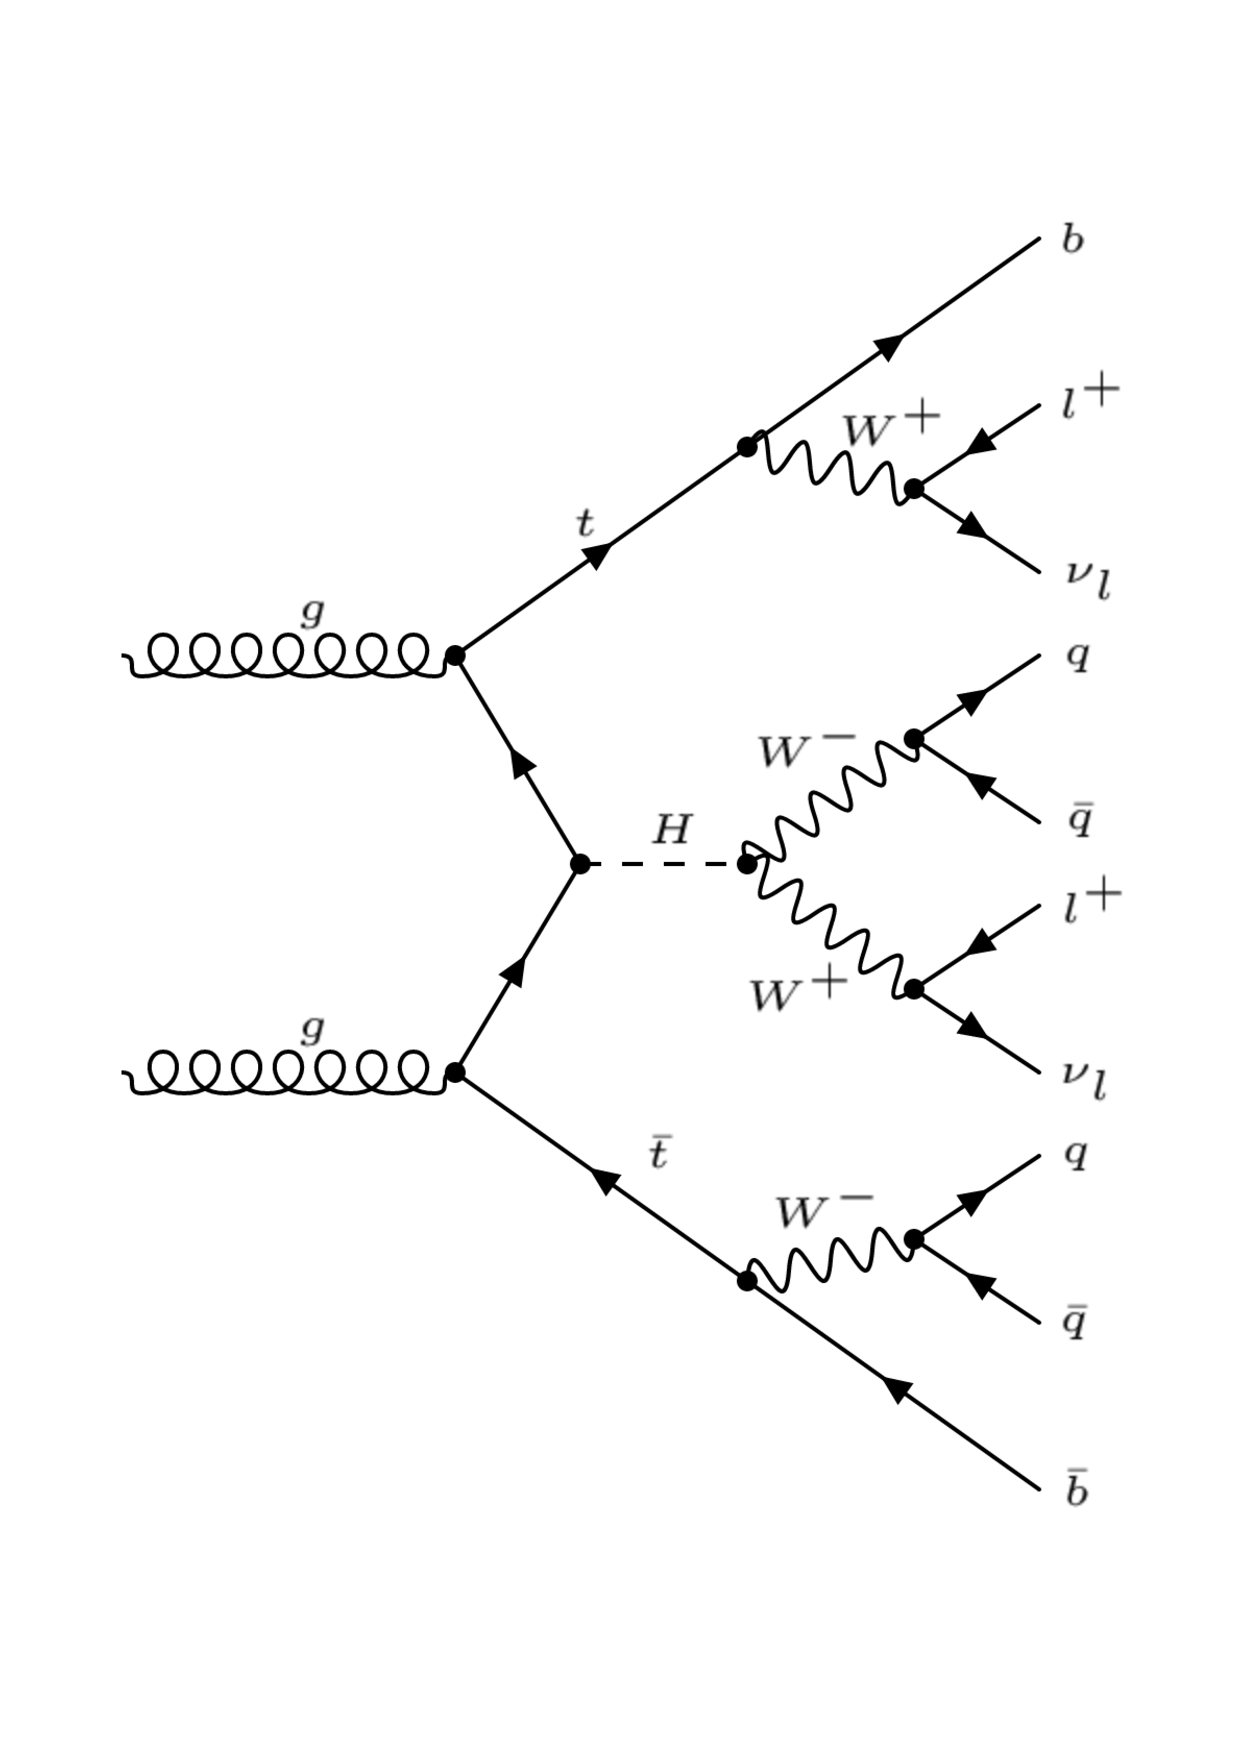
\includegraphics[width=0.5\textwidth]{ch1_figs/feynman_diagram_ttH_HWW_2lss.pdf}
   \caption{A feynman diagram of the primary signal process.}
   \label{fig:intro_feyn}
 \end{center}
\end{figure}

There are several reasons for considering \tth events with multiple lepton final states. The primary experimentally-driven reason is due to the efficiency with which
CMS identifies and reconstructs charged leptons. Reconstructing electrons and muons accurately is far easier compared to reconstructing jets,
which will be discussed in the following chapters. 
From a theoretical perspective, the bb decay mode of the Higgs is the most desirable having the largest branching fraction, however this is balanced by the large
uncertainties and experimental difficulty of accurately identifying and reconstructing jets with CMS.
Finally, there tend to be smaller backgrounds capabable of producing multiple leptons consistent with \tth with respect to other Higgs decay modes. 

%%DISCUSSION OF PREVIOUS \tth RESULTS

The results presented here build on previous measurements of the top-Higgs Yukawa coupling that were performed in \tth analyses by both ATLAS and CMS.
The initial searches analyzed 20 fb$^{-1}$ of 8 TeV pp collisions during Run I of the LHC. Combining the results of Higgs decay channels of bb, $\gamma\gamma$,
and leptonic final states produced a signal strength of $\mu$ = 2.8 $\pm$ 1.0, where $\mu$ = $\sigma/\sigma_{SM}$. The multilepton channel alone
observed $\mu$ = 3.7$^{1.6}_{1.4}$~\cite{jhep_tth}. Subsequent iterations of the multilepton analysis were performed again on 13 TeV pp collisions from Run II
of the LHC, the most recent signal strength observations are $\mu$ = 2.0$^{0.8}_{0.7}$, corresponding to 12.9 fb$^{-1}$, and the subsequent analysis on the full
2016 dataset on which this dissertation is based, and $\mu$ = 1.5 $\pm$ 0.5 ,corresponding to 35.9 fb$^{-1}$.


% % uncomment the following lines,
% if using chapter-wise bibliography
%
% \bibliographystyle{ndnatbib}
% \bibliography{example}

%
% Modified by Megan Patnott
% Last Change: Jan 18, 2013
%
%%%%%%%%%%%%%%%%%%%%%%%%%%%%%%%%%%%%%%%%%%%%%%%%%%%%%%%%%%%%%%%%%%%%%%%%
%
% Modified by Sameer Vijay
% Last Change: Tue Jul 26 2005 13:00 CEST
%
%%%%%%%%%%%%%%%%%%%%%%%%%%%%%%%%%%%%%%%%%%%%%%%%%%%%%%%%%%%%%%%%%%%%%%%%
%
% Sample Notre Dame Thesis/Dissertation
% Using Donald Peterson's ndthesis classfile
%
% Written by Jeff Squyres and Don Peterson
%
% Provided by the Information Technology Committee of
%   the Graduate Student Union
%   http://www.gsu.nd.edu/
%
% Nothing in this document is serious except the format.  :-)
%
% If you have any suggestions, comments, questions, please send e-mail
% to: ndthesis@gsu.nd.edu
%
%%%%%%%%%%%%%%%%%%%%%%%%%%%%%%%%%%%%%%%%%%%%%%%%%%%%%%%%%%%%%%%%%%%%%%%%


%
% Chapter 2
%

\chapter{THEORETICAL BACKGROUND}
\section{Introduction to the Standard Model}
The Standard Model (SM) of particle physics is one of the most elegant descriptions of nature available. It explains three of four fundamental forces via gauge symmetries, while characterizing unknown matter into
separate generations of particles called quarks and leptons. Since its inception in the early 1960s, the SM has predicted the existence of every fundamental particle that has been discovered to-date.
The SM distills the real-world observables matter and energy into discrete elementary particles and their kinematics. The SM is the theory on which all of the following research is based, and also the theory and hypothesis that is being tested.

\subsection{Particle Content}
The particles in the SM are first characterized by their intrinisic angular momentum, more commonly referred to as spin. Particles with half-integer spin, quantized in units of Planck's constant $\hbar$, are fermions, while particles with integer spin are bosons.
This distinction is important because the spin values govern behavior and interactions of the statistics of sets of collections of particles. 

The fermions in the SM are the most fundamental examples of matter in nature. Fermions behave and interact according to Fermi-Dirac statistics, and obey the Pauli exclusion principle. Fermions are further categorized, based on their primary interaction mechanism,
into quarks and leptons. There are six different flavors of quarks in the SM, the up and down, the charm and strange, and the top and bottom quarks are organized into three generations of doublets below.
\begin{equation}
\binom{u}{d} \;\;\; \binom{c}{s} \;\;\; \binom{t}{b}
\end{equation}
\noindent An increasing mass (from left to right) distinguishes each generation, while the upper and lower elements of each doublet are distinguished by an electric charge of +2/3 and -1/3 respectively in each generation. Quarks interact via the strong, weak, and
electromagnetic interactions. Quarks also carry a color charge, which can assume one of three values (red, blue, green) as a result of the strong interaction described by Quantum Chromodynamics (QCD). The leptons in the SM can also be arrange into three increasingly
massive generations of doublets.
\begin{equation}
\binom{e^{-}}{\nu_{e}} \;\;\; \binom{\mu^{-}}{\nu_{\mu}} \;\;\; \binom{\tau^{-}}{\nu_{\tau}}
\end{equation}
\noindent The upper elements in each lepton doublet are the familiar electron, and the less familiar but much heavier, muon and tau. Due to their increased mass, the muon and tau have very short lifetimes which causes them decay rapidly
to lighter, more stable particles. The electron, muon, and tau all have the same electric charge of -1. The lower elements in each doublet are the lightweight and electrically neutral counterparts called neutrinos, which also come in three
flavors; the electron-neutrino, the muon-neutrino, and the tau-neutrino. While the electron, muon, and tau interact via both the electromagnetic and weak force, neutrinos interact only through the weak force. Neutrinos are characterized by
how weakly they interact. They interact so weakly that they are able to pass through all of planet earth without a single interaction. This property makes it impossible to directly detect their presence at CMS. 

\begin{figure}[hbtp]
 \begin{center}
   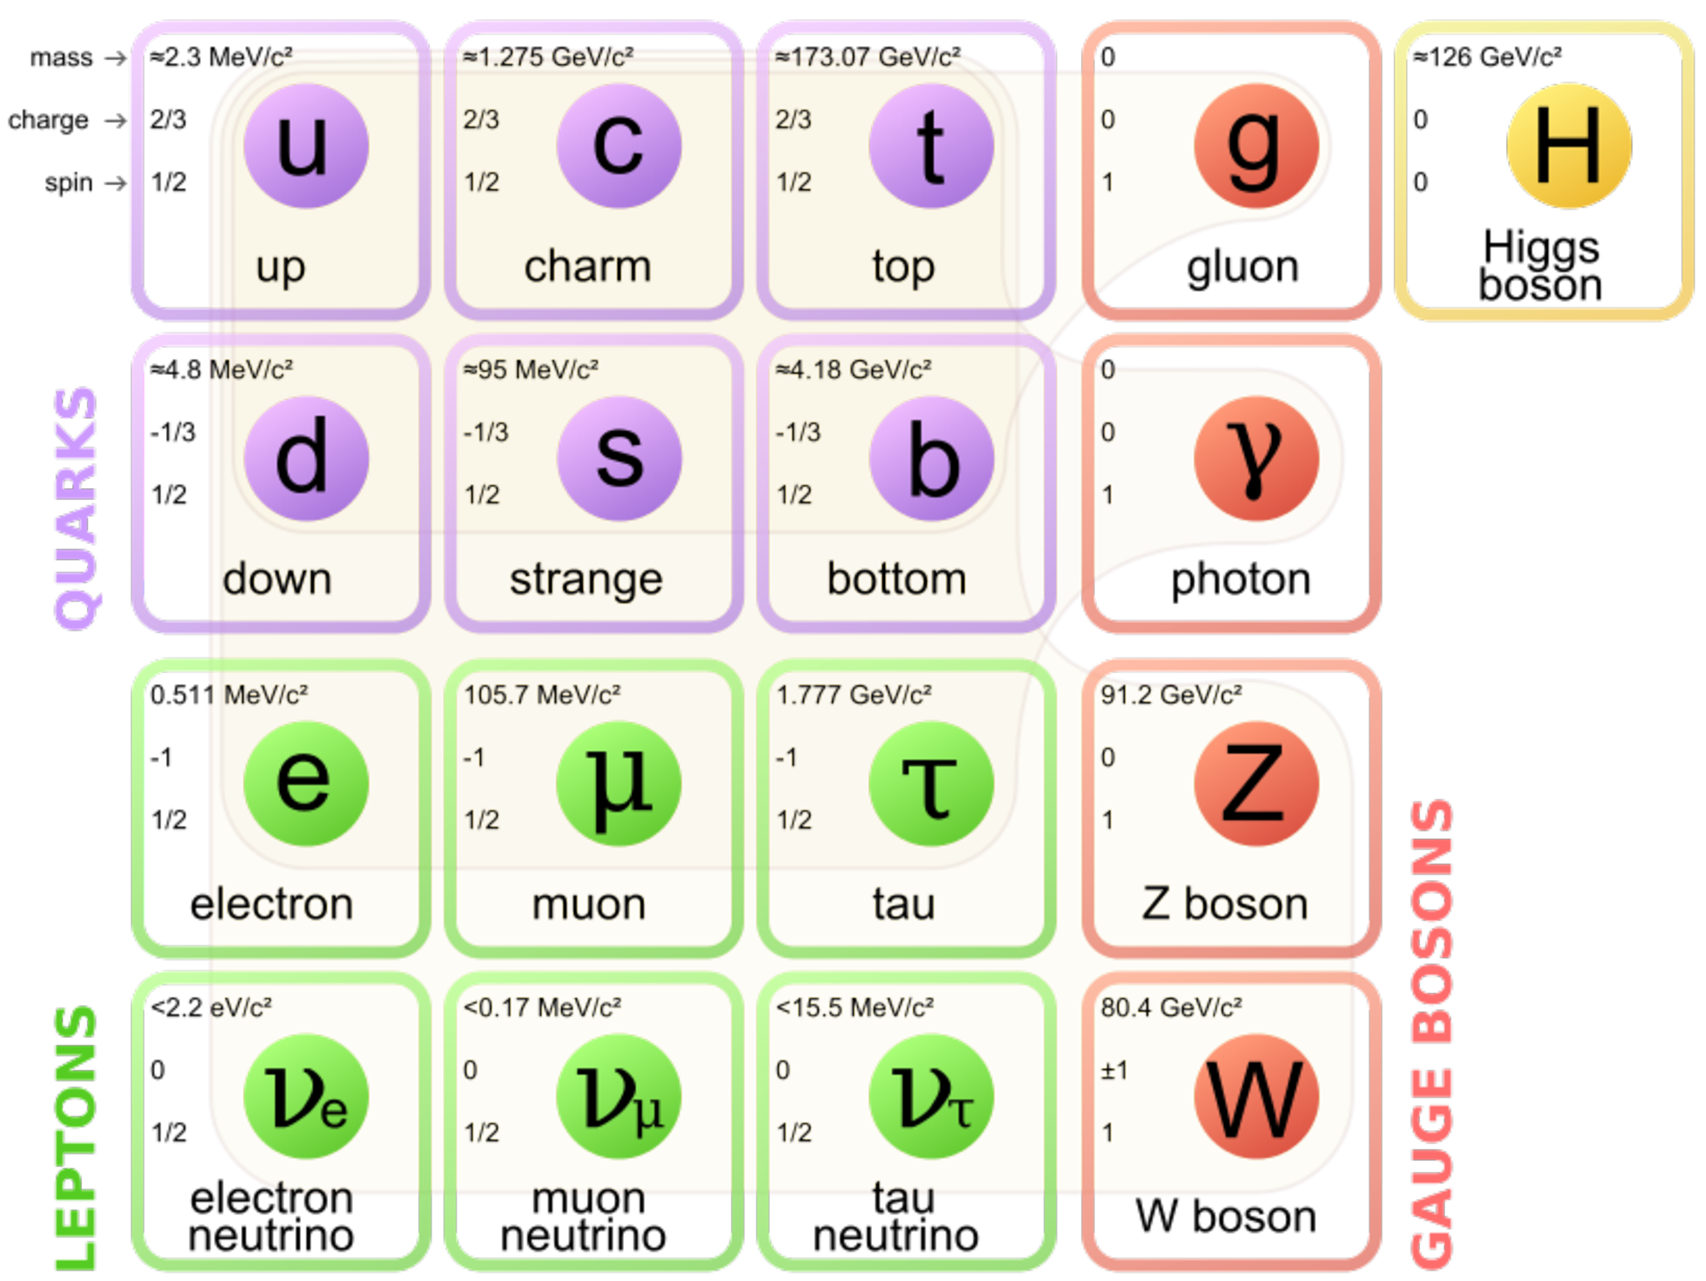
\includegraphics[width=0.8\textwidth]{ch2_figs/sm_particles_periodic_table.pdf}
   \caption{A sumamry of all elementary particles and their interactions in the Standard Model~\cite{sm_table}.}
   \label{fig:sm_periodic_table}
 \end{center}
\end{figure}

The bosons in the SM are also fundamental, but are not examples of matter. Bosons are characterized by their integer-quantized angular momentum and behave according to Bose-Einstein statistics. There are five elementary SM bosons, the four force-carrying gauge
bosons, and one scalar (spin-0) boson that was recently discovered in 2012, known as the Higgs boson. The four forces (strong, weak, electromagnetic, gravity) through which particles interact are all carried by the corresponding gauge bosons, with the exception
of gravity. The SM currently does not explain gravity because there is no SM particle that carries its force. The gauge boson believed to be responsible for this, the graviton, has yet to be discovered and likely exists in a mass range far beyond the reach of
the LHC. The strongest of the four forces, the appropriately-named strong force is carried by the gluon. Gluons are spin-0, electrically neutral, massless, and carry a color charge. Gluons mediate the strong force through which quarks interact. Due to the nature of
color charge and confinement, gluons keep the quarks inside protons and neutrons glued together, confined inside the proton. Additionally, strong force also binds protons and neutrons together to form nuclei of atoms. Any particle carrying color charge is capable
of strong interactions. 
The photon is the gauge boson that mediates the next strongest interaction, the electromagnetic force. The photon is massless, spin-1, electrically neutral, and travels at the speed of light. Aside from gravity, the electromagnetic force is the most familiar,
responsible for keeping electron orbitals bound to nuclei, forming atoms, and it is also responsible for the attractive and repulsive forces that bond atoms together into molecules. Any particle carrying electric charge is capable of interacting electromagnetically.
The weakest force explained by the SM, the appropriately named weak force is mediated by the massive W and Z gauge bosons. There are two types of weak interactions, charged and neutral.
There are two W bosons, W$^+$,W$^-$ which identical except differ by electric charges of +1 and -1 respectively. The spin-1 W boson has a mass of 80.4 GeV~\cite{LopesdeSa:2012ak}, and mediates the weak charged interaction.
The electrically neutral, spin-1 Z boson weighs 91.2 GeV and mediates the weak neutral interaction. The nuclear decay of unstable atoms, which is harnessed for nuclear power, is possible thanks to the weak interaction.
The final elementary SM boson is the Higgs. The Higgs is a massive spin-0, electrically neutral boson that interacts with both fermions and other bosons and weighs approximately 125 GeV. While the Higgs doesn't mediate a force, it does represent a field, and the
mechanism by which elementary particles obtain masses. The Higgs boson and the origins of mass will be explained the coming sections. 

\subsection{Fields and Symmetries}
The notion of symmetry is of central importance to the SM. The SM successfully describes three of the fundamental forces, which were each previously described separately by their own gauge field theory, and unites them into one consistent description
of nature. 

The first gauge field theory was Quantum Electrodynamics, which described the electromagnetic field and its force carrying gauge boson, the photon. This theory 

\section{Electroweak Symmetry Breaking and the Higgs Boson}


\section{ttH}


% % uncomment the following lines,
% if using chapter-wise bibliography
%
% \bibliographystyle{ndnatbib}
% \bibliography{example}

%
% Chapter 3
%

\chapter{EXPERIMENTAL APPARATUS}
\label{chap:detector}

\section{The Large Hadron Collider}
\label{sec:lhc}
The most powerful machine of its kind, the Large Hadron
Collider (LHC) accelerates and collides particles
at high center-of-mass energies producing rare
particles and interactions that would be otherwise unobservable
in the laboratory, making it the best tool available for producing \tth
processes. The LHC is a circular particle accelerator/collider. Measuring 27 km
in circumference, it collides beams of protons in head-on collisions       
at a center-of-mass energy of 13 TeV.

Originally conceived in the early 1980s and approved in 1994, the LHC was designed to replace the then-operating
Large Electron Positron Collider (LEP), re-using the same underground tunnel. Located just outside Geneva, Switzerland, at the Center for European Nuclear Research (CERN),
the LHC stretches across the border into France. There are four detectors positioned around the LHC: ALICE, ATLAS, CMS, and LHCb. The two general purpose,
functionally-equivalent detectors are ATLAS and CMS, while ALICE studies heavy ion collisions, and LHCb focuses on flavor physics. 
The motivation for having two equivalent detectors is to provide cross checks on results, as each result is produced with separate analysis teams, studying separate collisions
recorded with a separate detector. Each detector is centered on an interaction point, where the beams are steered into each other to produce collisions. 
The LHC itself is technically the final element in a series of accelerators
that bring particle beams from rest to successively higher energies. This system of
of accelerators, referred to as the LHC Accelerator Complex is depicted below in
Figure~\ref{fig:lhc_complex}.

The acceleration is accomplished with radio frequency (RF) cavities. RF cavities are a linear series of cylindrical conductors,
which sustain a resonant electromagnetic field produced by a generator. As 
charged particles pass through the cavities, they experience a force
(acceleration) from the resonant alternating field in each cavity. This acceleration process begins with hydrogen gas in the linear accelerator
(LINAC 2). The hydrogen atoms in the gas are stripped of electrons
in an applied electric field, leaving only protons, which are then accelerated
along the linear beam pipe with RF cavities to an energy of 50 MeV. After the LINAC, the beams of protons enter the Proton Synchrotron Booster rings where
they are accelerated to 1.4 GeV, before reaching the Proton
Synchrotron (PS). The circular PS, measuring more than 600 m
in circumference, accelerates the beams to 25 GeV before injection into the
larger, Super Proton Synchrotron (SPS). The SPS at over 7 km around, provides the final
acceleration before the beams reach the LHC at an energy 450 GeV. The SPS injects the beams into
the LHC in opposite directions to facilitate collisions later. After the beams are fully injected, the LHC ramps the beam energy to 6.5 TeV per beam, providing 13 TeV center-of-mass proton collisions~\cite{lhc_bluebook}.

The beam pipes of the entire accelerator complex are kept at an ultra high vaccuum
to avoid detrimental beam interactions before the collisions. Since the beams are made up of protons which have electric charge,
they can be focused and steered around the LHC with 392 quadrupole and 1232 dipole superconducting magnets.
To accomplish this, the magnets produce a field of over 8 Tesla. This is possible thanks to the
superconducting niobium-titanium (NbTi) coils which are cooled with superfluid helium-4. These
magnets operate at 1.9 K allowing them to carry a current of over 11,000 amperes. In addition to
the LHC, similar superconducting magnets are used throughout the accelerator complex~\cite{lhc_bluebook}.

Inside the LHC, the beams travel in opposite directions in separate but adjacent pipes inside of the superconducting magnets.
As a result of the RF cavity acceleration, the beams are comprised of individual `bunches' of protons.
There are over 2800 bunches in each beam, with each bunch spaced 25 ns apart. This spacing is choosen to
produce as many bunch crossings as possible, without overloading
the detector instrumentation and data acquisition. Extra space is placed at certain intervals of bunches
both for injection purposes and to allow for additional time to activate special kicker magnets that dump t/e beams. The extra space, up to 3 $\mu$s, is 
called the abort gap. Of the over 2800 bunches in each beam, there are approximately $10^{11}$ protons in each bunch, but due to the small cross section of the protons,
only approximately 20 collisions occur in each bunch crossing. The beams travel around the LHC over 11,246 times per second, over 99.99$\%$ the speed of light. 
This translates to around 600 million collisions per second ~\cite{lhc_bluebook}.

The LHC's ability to collide protons at the energies and intensities described above make it an excellent tool for producing interesting
and rare physics processes like \tth.
A sufficient center-of-mass collision energy is needed to produce new, heavy particles.
With the current center-of-mass collision energy at 13 TeV, any particle with mass less than or equal to this, is 
technically within reach of the LHC. While this is technically the upper bound, the practical bound on a new particle mass is substantially smaller,
since the proton collisions are actually collisions of the individual partons\footnote{Partons refer here to any quark or gluon. The phrase was originally
coined by Richard Feynman, as an individual parton makes up `part' of a meson or baryon.} inside the protons, and the partons carry fractions of the total proton
momentum\footnote{The LHC is, on occasion, referred to as a gluon collider. This is due to gluons being the most likely parton to carry a non-negligible fraction of the proton momentum, thus
being the most likely parton to participate in a hard-scatter collision. This is why many physics processes studied at the LHC, including \tth, have incoming gluons in the initial state.}.
The momentum fractions carried by each of the partons, known as Parton Distribution Functions (PDFs) are determined based on inelastic scattering experiments, and theoretical calculations, since they
vary with momentum transfer. Examples of the PDFs used in this analysis are in Figure~\ref{fig:nnpdf}. 

\begin{figure}[hbtp]
 \begin{center}
   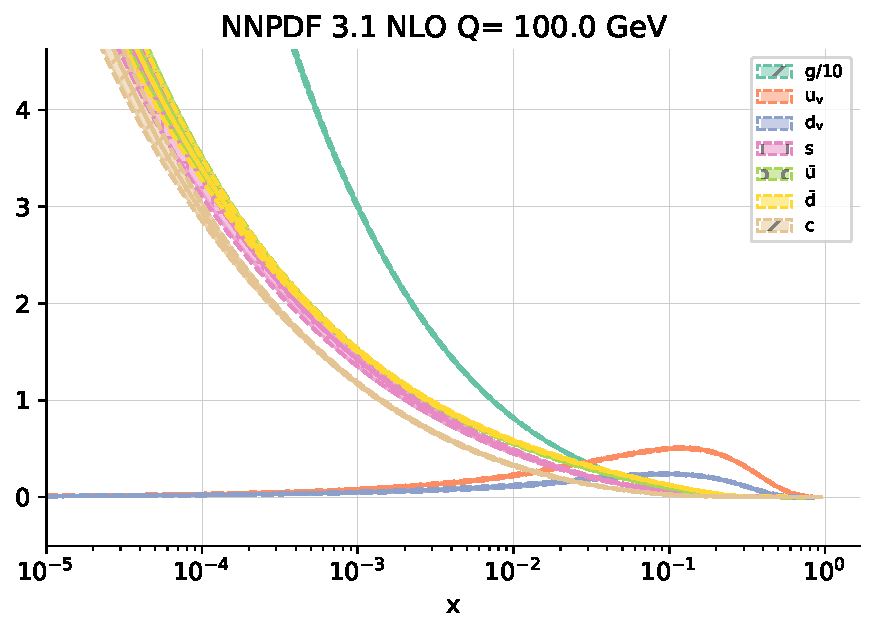
\includegraphics[width=0.9\textwidth]{ch3_figs/nnpdf3p1_nlo_q100.pdf}
   \caption[NLO parton distribution function for the proton at Q = 100 GeV]{NLO parton distribution function for the proton at momentum transfer of 100 GeV.
     The x-axis represents the fraction of the total proton momentum carried by a given parton type while the y-axis corresponds to relative
     frequency\cite{nnpdf3}.}
   \label{fig:nnpdf}
 \end{center}
\end{figure}

\noindent Because many interesting physics processes are exceedingly rare (small cross section), many collisions
are needed. The quantity used to describe the rate of collisions is luminosity.
Described in equation~\ref{eqn:lumi_inst} below, instantaneous luminosity represents the number of collisions (events) occuring per unit time~\cite{lhc_bluebook}.

\begin{equation}
\label{eqn:lumi_inst}
\mathcal{L}_{inst} = \frac{N_{b}^{2}n_{b}f_{\textnormal{rev}}\gamma}{4\pi \epsilon_{n} \beta^{*}}F
\end{equation}

Where $N_{b}$ is the number of protons per bunch, $n_{b}$ is the total number of bunches, $f_{\textnormal{rev}}$ is the number of beam revolutions around the LHC per
second, $\gamma$ is a relativistic factor, $\epsilon_{n}$ is factor related to beam emittance, $\beta^{*}$ is the beta function, which is related to the transverse beam size
at the interaction point, and
$F$ describes the factor related to the crossing angle of the beams. Because not every collision can be recorded, knowing the total number of collisions is critically important
to every analysis at an LHC collider experiment. The integrated luminosity is the time integral of the instantaneous luminosity. Combining this with the proton-proton inelastic
cross section, $\sigma_{pp}$, the number of collisions occurring in time interval $t$ is calculated in equation~\ref{eqn:num_coll} below. 

\begin{equation}
\label{eqn:num_coll}
N_{pp} = \int \sigma_{pp}\mathcal{L}_{inst}dt 
\end{equation}


\begin{figure}[hbtp]
 \begin{center}
   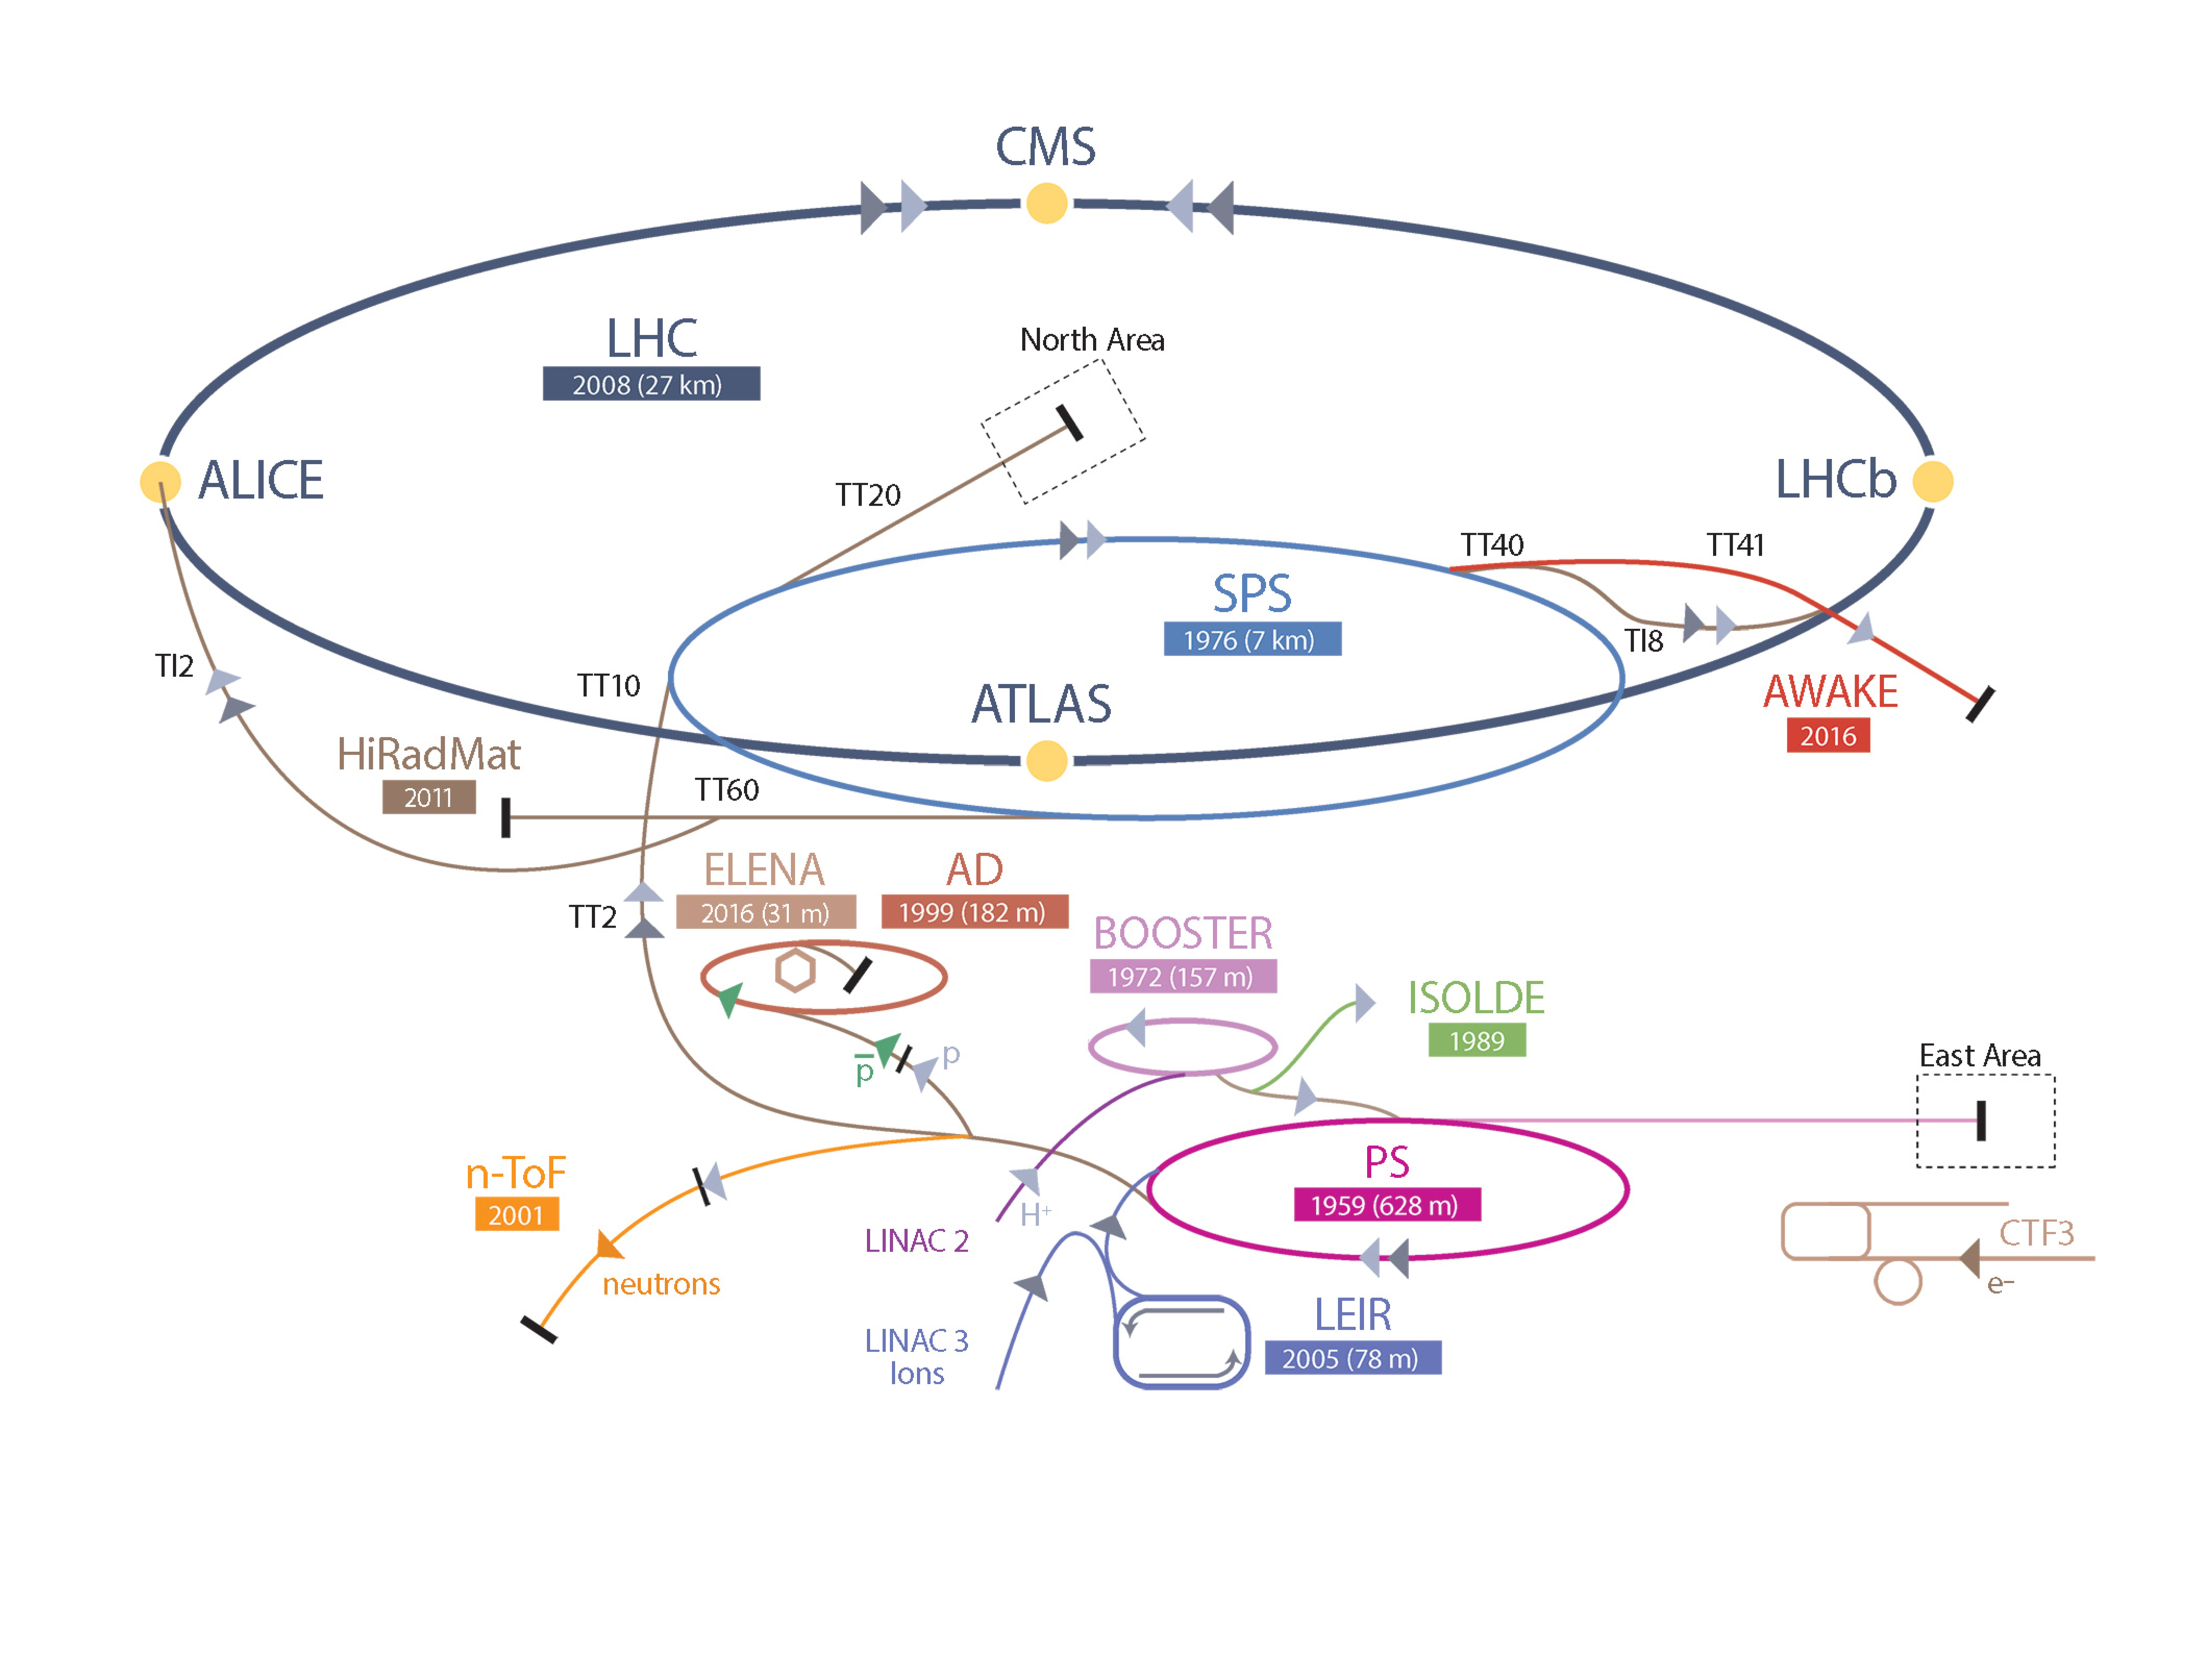
\includegraphics[width=0.9\textwidth]{ch3_figs/lhc_complex.pdf}
   \caption[Overview of the LHC accelerator complex]{An overview of the LHC accelerator complex~\cite{lhcfig}.}
   \label{fig:lhc_complex}
 \end{center}
\end{figure}


\section{The Compact Muon Solenoid (CMS) Detector}
\label{sec:cms}
100 m beneath the town of Cessy, France, sits the Compact Muon Solenoid (CMS) detector, a multi-purpose particle detector designed
to record and identify particles from collisions produced by the LHC.
CMS is comprised of layers of subdetectors which are connected to readout electronics and the trigger and data acquisition systems.
The various subdetectors record information about the collision, while the trigger and
data acquisition systems record and save the collisions. The acronym CMS comes from being more compact than its sister detector ATLAS, at 15 m in diameter and
over 21 m long. The muon in the acronym comes from the fact that detecting muons is among the most important tasks of the experiment. The solenoid part of the name is due
the powerful solenoid magnet which is crucial for particle tracking and identification. 
CMS is cylindrical in shape, as pictured in Figure~\ref{fig:cms_overview}. The various subdetectors and components are described in more
detail below. 

%% \begin{table}[hbtp]
%% \centering
%% \caption{Quantitative Summary of the CMS Detector}
%% \begin{tabular}{lcc}
%% \hline
%% Detector & Summary  \\
%% \hline
%% CMS total weight & 14000 tons  \\
%% %\hline
%% CMS diameter & 15.0 m \\
%% %\hline
%% neutralEmEnergyFraction (NEF)& \textless 0.99 \\
%% %\hline
%% neutralHadronEnergyFraction (NHF)& \textless 0.99 \\
%% %\hline
%% chargedHadronEnergyFraction (CHF) & \textgreater 0 \\
%% %\hline
%% number of charged hadrons (NCH) & \textgreater 0 \\
%% %\hline
%% N$_{constituents}$ & \textgreater 1 \\
%% \hline
%% \end{tabular}
%% \label{tab:JetTable}
%% \end{table}


\begin{figure}[hbtp]
 \begin{center}
   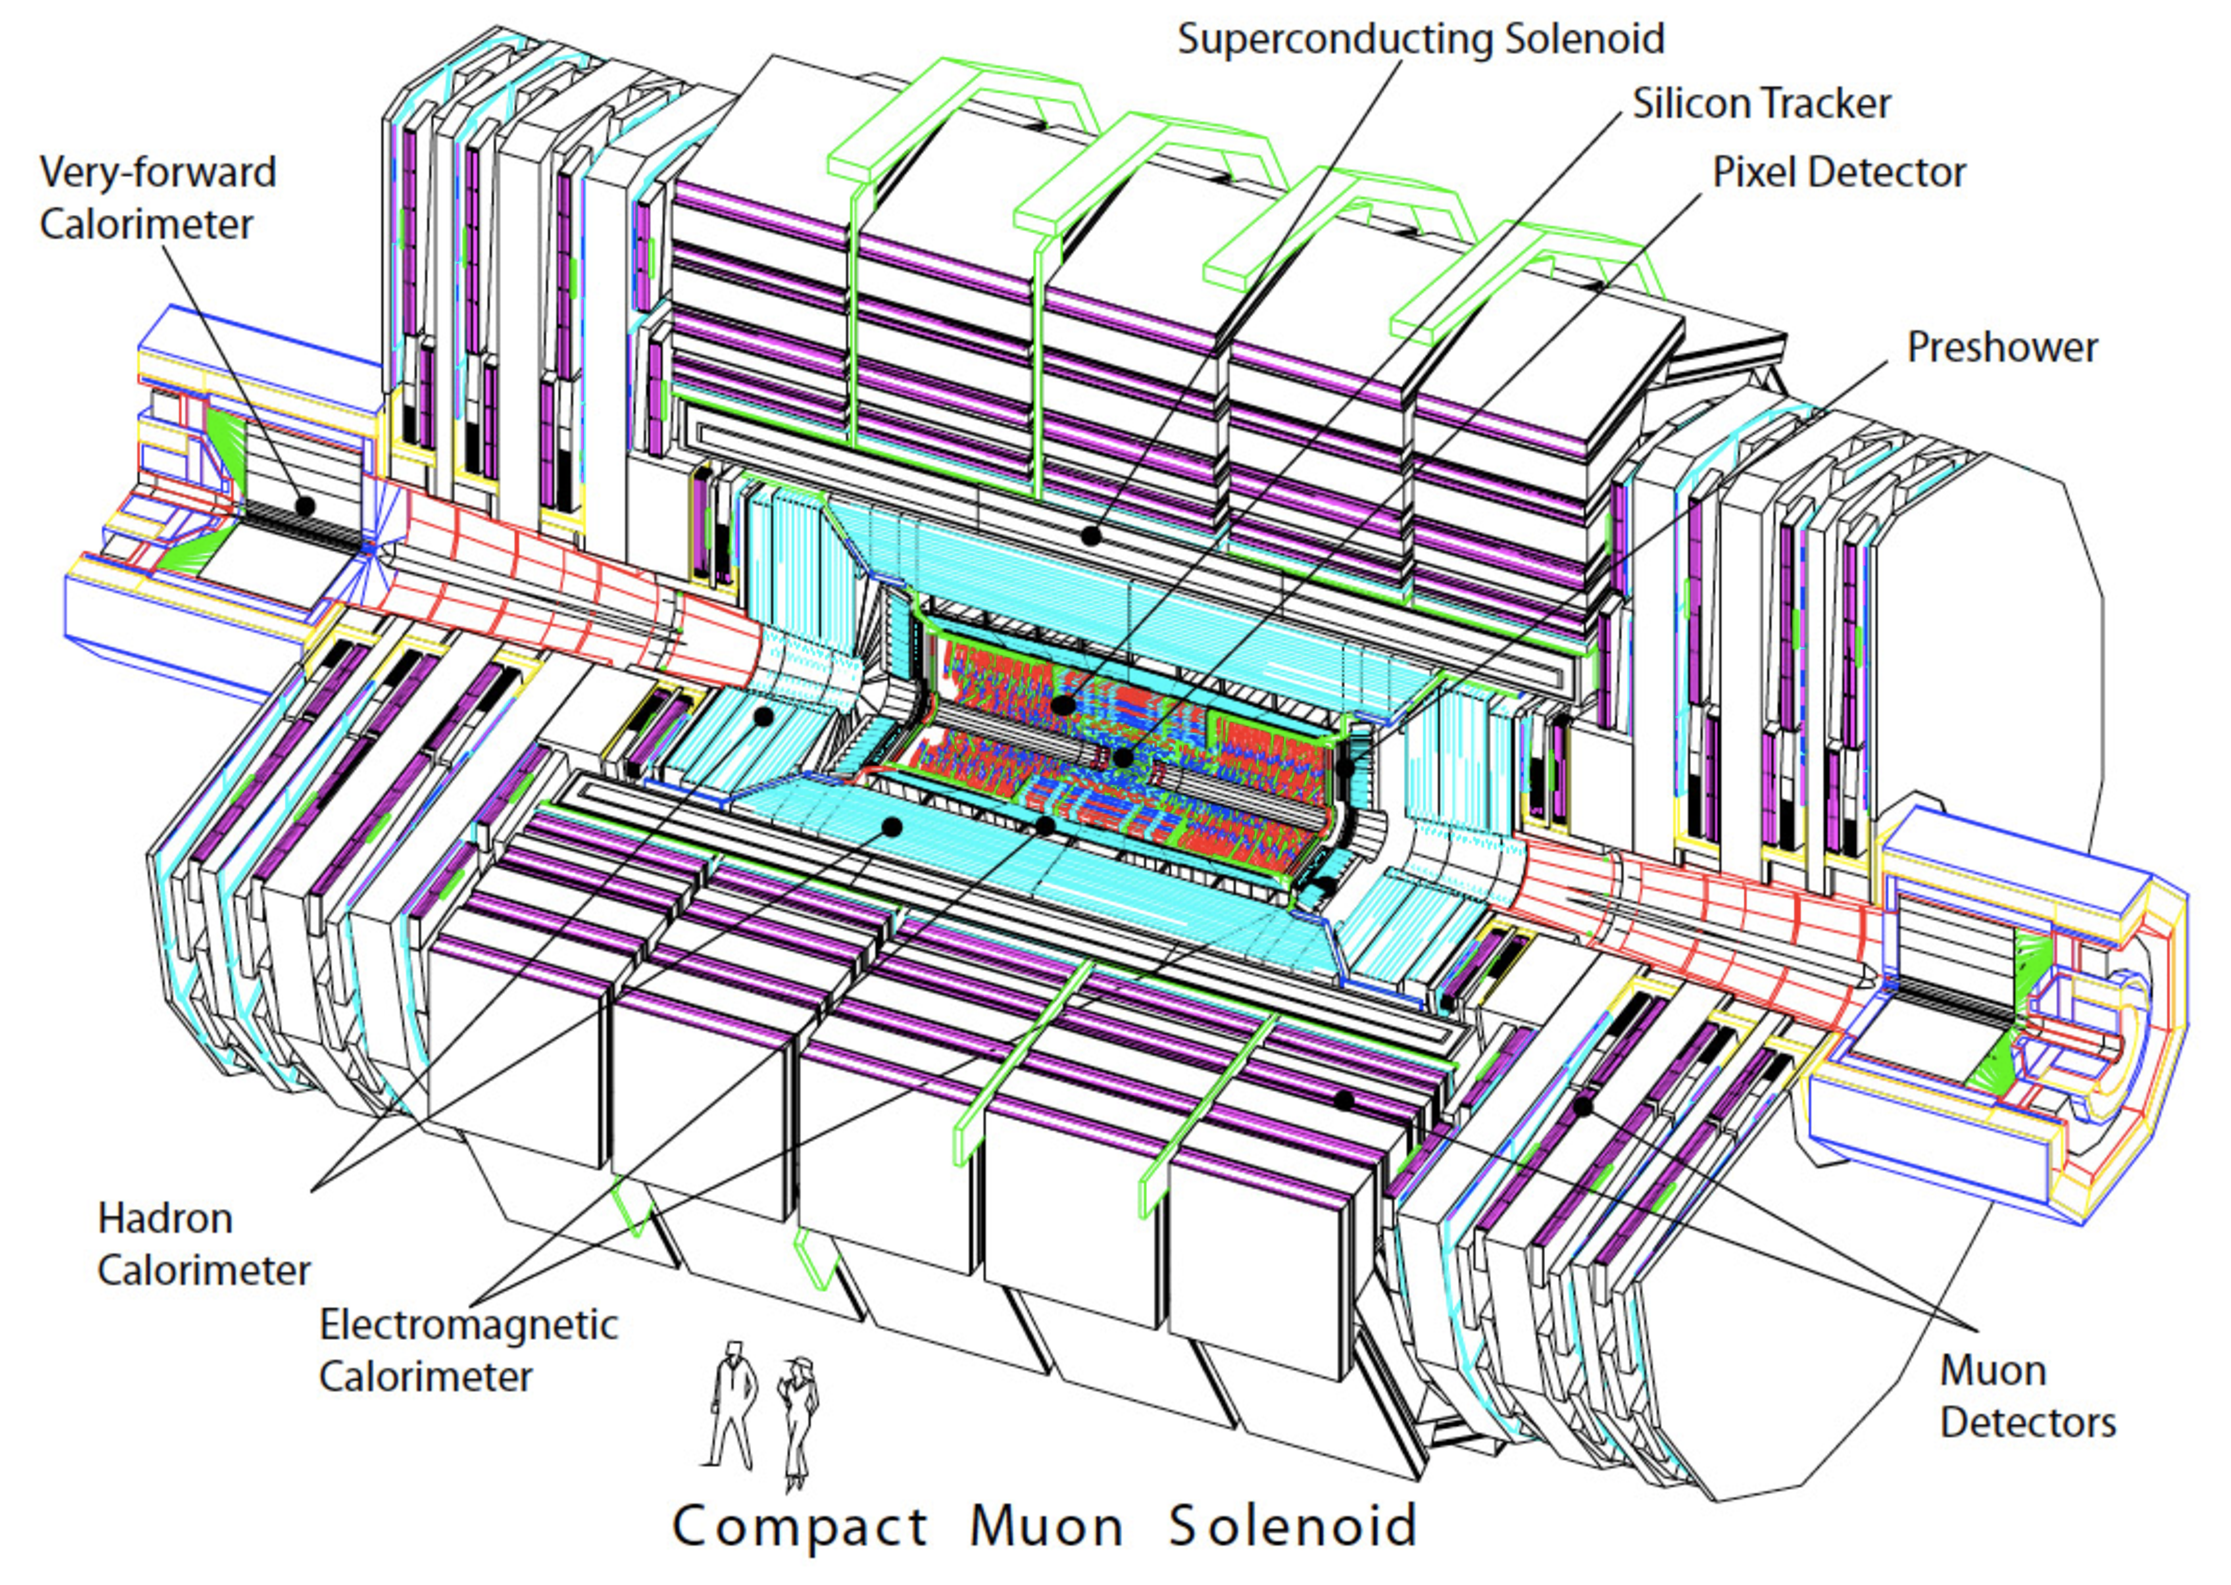
\includegraphics[width=0.9\textwidth]{ch3_figs/cms_overview_white.pdf}
   \caption[Overview of the CMS detector]{A qualitative overview of the CMS detector~\cite{cms_bluebook}.\label{fig:cms_overview}}
 \end{center}
\end{figure}

\subsection{Coordinate System}
Due to the geometry and symmetry of the collisions produced inside CMS, a special coordinate system is used for simplicity. With the origin at the interaction point,
the y-axis in the vertical direction, the z-axis parallel to/along the beam direction, and the x-axis in the horizontal direction perpendicular to both the y
and z axes. In the transverse x-y plane, the azimuthal angle formed with respect to the x-axis is $\phi$. In the y-z plane, the angle formed with respect to the z-axis
is $\theta$. The number of particles traveling through a given area, known as flux, increases towards the beam line, due to many more glancing collisons occurring
than head-on collisions. The particles from the collisions are moving relativistically. Because of this, a special coordinate $\eta = -\ln\tan(\theta/2)$, 
is used to describe the angle with respect to the z-axis, known as $pseudorapidity$. 
Finally, the transverse plane is of special importance for momentum and energy measurements due to energy/momentum conservation, since the head-on inelastic
pp collisions have only momentum in the z-direction.

\subsection{Tracker}
The CMS tracking system sits closest to the interaction point at the core of CMS and provides precise tracking information from its millions of silicon sensors.
The tracking system is comprised of two concentric cylindrical subdetectors, the pixel and strip detectors, which are named after the geometry of the sensors they use. 
The pixels provide the highest granularity tracking information, essential for distinguishing between collision vertices, and sit nearest to the interaction point,
inside of the strip detector.
The strips provide slightly less resolution compared with the pixels, since they sit further from the interaction point. There is approximately one
radiation length\footnote{A radiation length is defined as the distance an energetic electron travels in material before losing all but 1/e of its
initial energy due to bremsstrahlung emission~\cite{radiation_length}.}
of tracker material (pixels + strips) between the interaction point and the beginning of the next subdetector, the ECAL.
The total detector area of the tracking system (pixels+strips) sums to more than a tennis court of silicon.

As a charged particle travels through a silicon sensor (pixel or strip), it ionizes a small fraction of the silicon atoms, releasing electrons from the valence band of n-type or p-type
semiconductor,
creating electron-hole pairs. A voltage is applied to the sensor, attracting the now free electrons, creating a small current. This current is measured and interpreted as a hit.
A small silicon pn junction is attached to the back of each sensor to read the voltage and send the hit information to the data acquisition system,
so the hit patterns can be reconstructed into particle tracks later.   
As the particles travel through successive layers of silicon sensors, they leave collections of hits.
The hits are measured with a precision of 10 $\mu$m, and the particle track is reconstructed from this collections of hits. 
Because the information from the tracker has such a high granularity, track reconstruction algorithms need more time than is feasable for trigger decisions
and are mostly performed offline.


\subsubsection{Pixel Detector}
The pixel detector is comprised of 65 million silicon pixels, allowing it to record
precise trajectories of the charged particles resulting from collisions. Precise tracking information is critical to differentiating nearby particles, and identifying
exactly where an interesting collision took place. 

\begin{figure}[hbtp]
 \begin{center}
   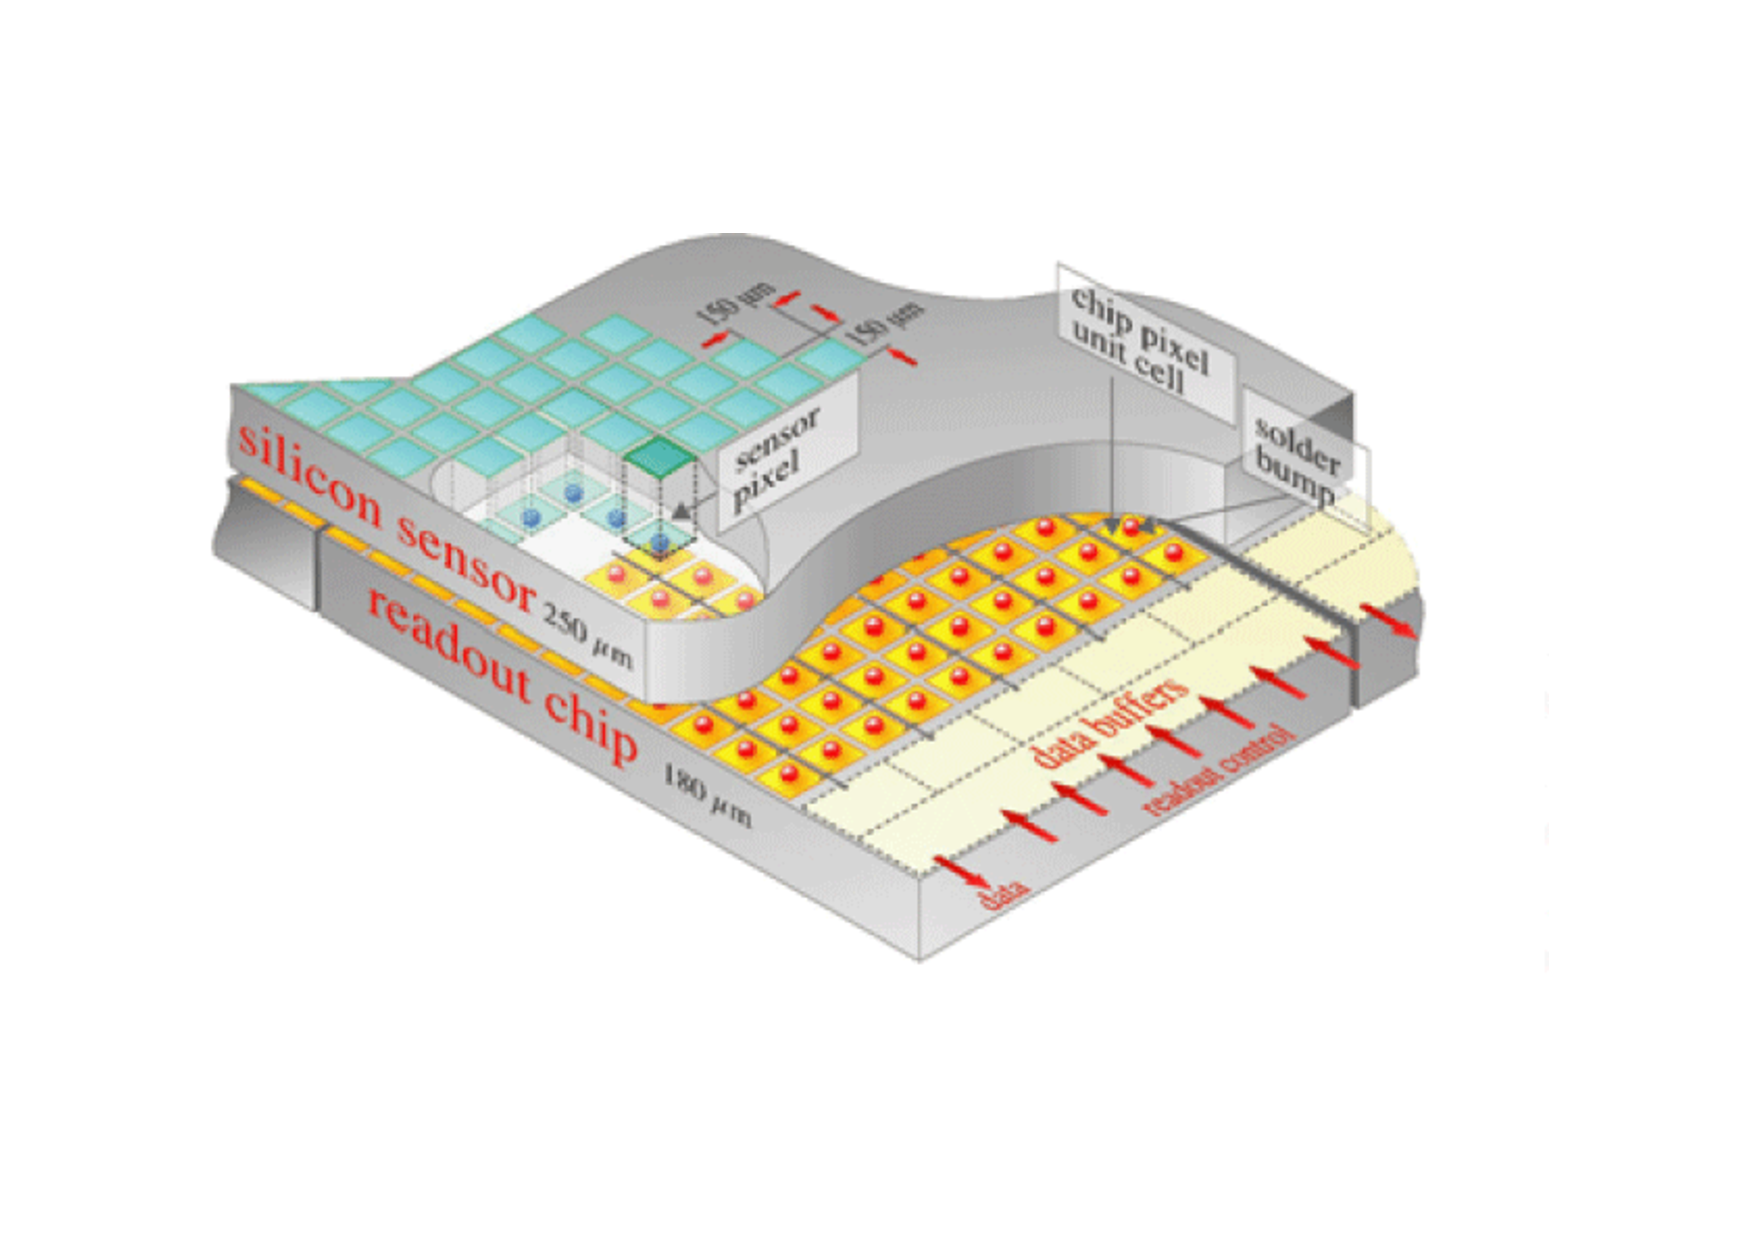
\includegraphics[width=0.85\textwidth]{ch3_figs/cms_pixel.pdf}
   \caption[CMS silicon pixel element]{An overview of a CMS pixel element~\cite{cms_pixel}.}
   \label{fig:cms_pixel}
 \end{center}
\end{figure}

\noindent The pixel detector is about the size of a shoe box and contains 3 layers at 4 cm, 7 cm, and 11 cm from the beam.
Silicon is used in the tracker over other materials, as it strikes the best balance between performance, radiation resistance, and affordability. 
Radiation resistance, also known as radiation hardness, is very important for the tracker as it sits only a few centimeters from the interaction point
receiving around 10 million particles per square centimeter per second.
Each silicon pixel measures 100 $\mu$m by 150 $\mu$m and is readout by an electronic chip bump-bonded to the back of each pixel. The layout of a pixel sensor is depicted in
Figure~\ref{fig:cms_pixel}.  

\subsubsection{Strip Detector}
Outside the pixel detector is the silicon strip detector. Here, silicon strips are favored over pixels as they are less costly, and the resolution provided by the pixels
is not necessary at greater distances from the interaction point, allowing for larger and fewer silicon modules.
The silicon strip detector consists of about 10 million strips in 10 layers, extending to 130 cm from the beam. 
The strip detector is comprised of 4 distinct sections of silicon strips, depicted in
Figure~\ref{fig:cms_tracker}. The outer most sections are the tracker outer barrel (TOB) and tracker end cap (TEC+,-) sections. 
Between the TOB and the pixels, sits the tracker
inner barrel (TIB) section, and the tracker inner endcaps (TID+,-).
The silicon strips in each section are different, specifically suited to that section.
Each silicon strip measures between 10-25 cm by 180 $\mu$m, depending on the position.
Precise tracking information is essential to measuring particle momenta and identifying particles in the strong magnetic field.

\begin{figure}[hbtp]
 \begin{center}
   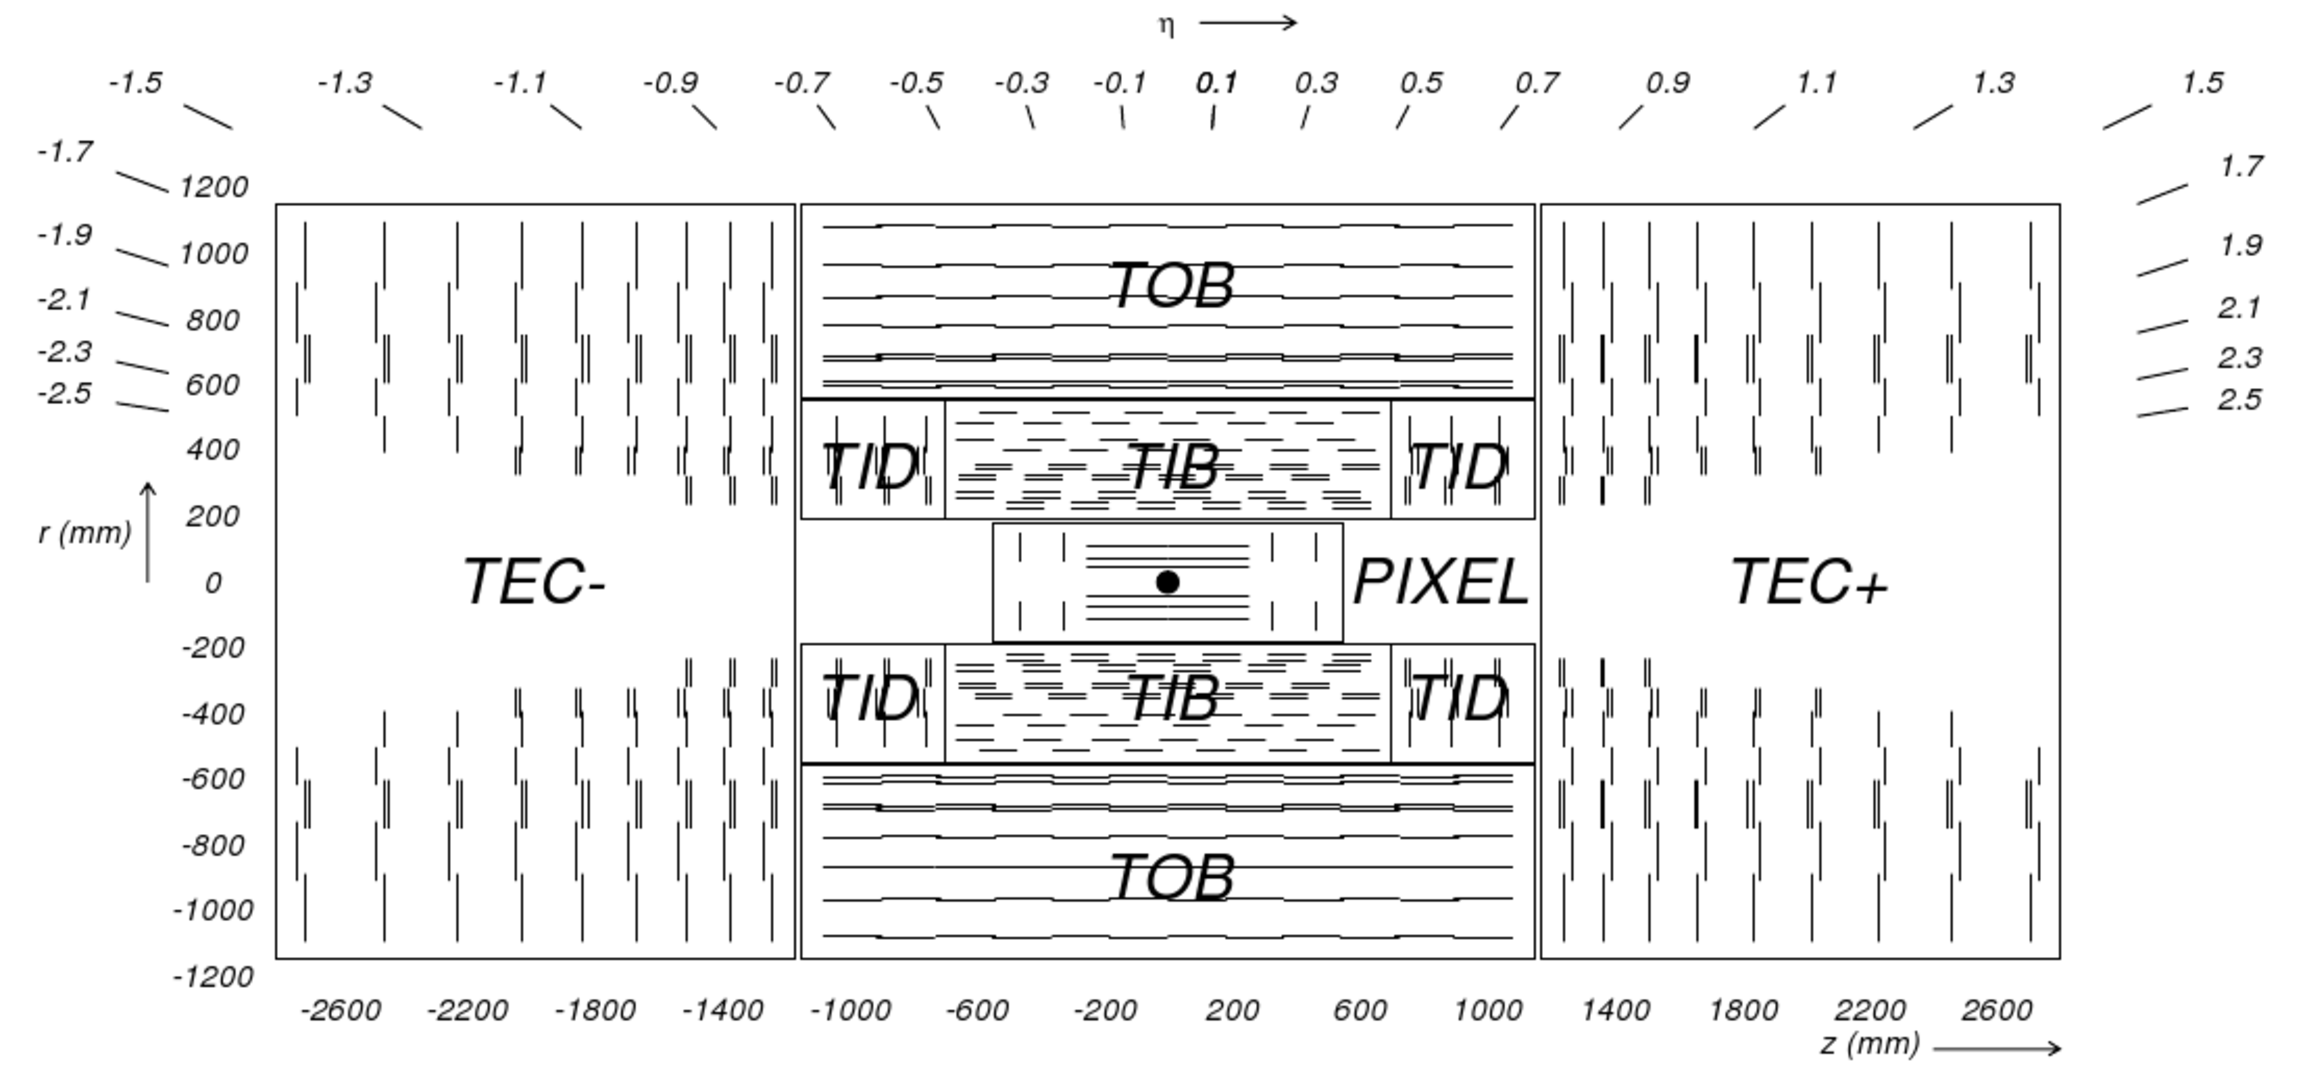
\includegraphics[width=0.6\textwidth]{ch3_figs/tracker_yz.pdf}
   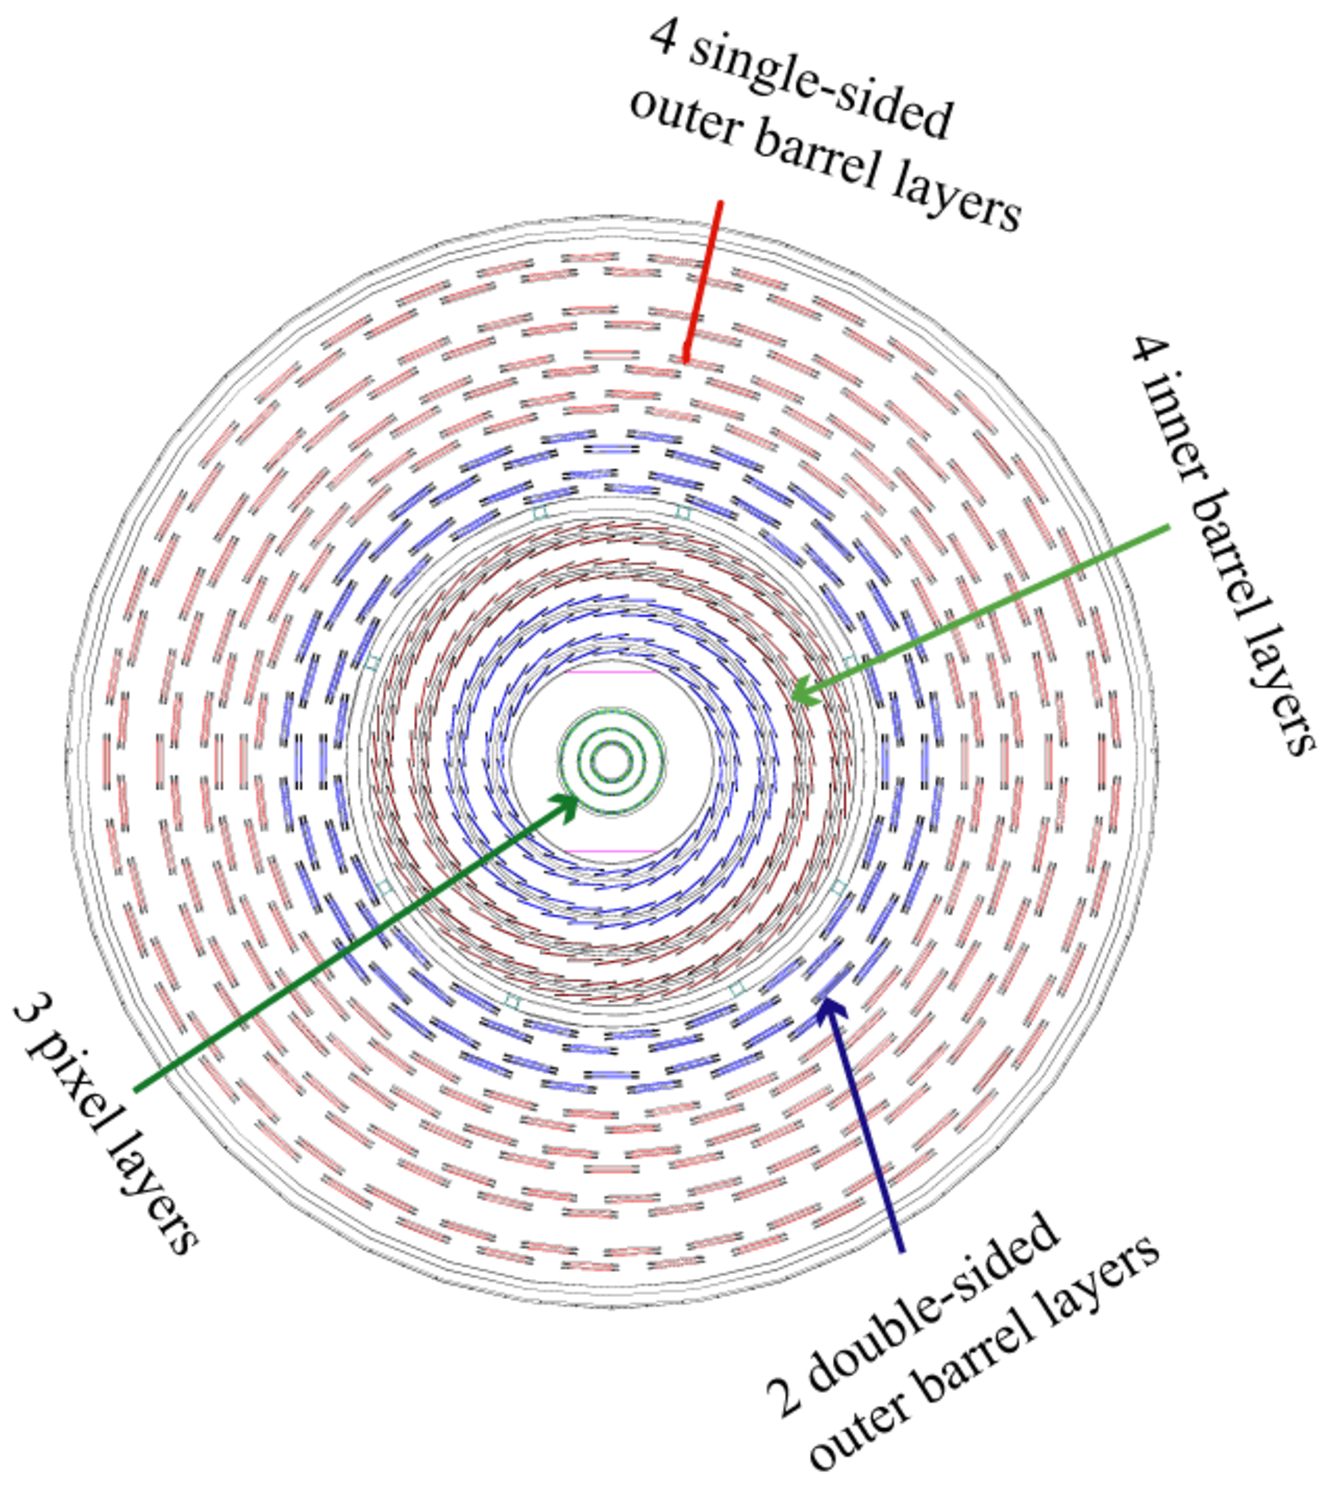
\includegraphics[width=0.25\textwidth]{ch3_figs/tracker_transverse_layers.pdf}
   \caption[The CMS silicon tracking system]{The CMS silicon tracking system including both the pixel and strip detectors in y-z plane (left), and transverse x-y plane (right)~\cite{cms_bluebook}.}
   \label{fig:cms_tracker}
 \end{center}
\end{figure}

\subsection{ECAL}
The Electromagnetic Calorimeter (ECAL) measures the energy of charged particles\footnote{The ECAL gets its name because it detects charged particles, which interact via the
electromagnetic force}. The ECAL is situated immediately outside the tracker
and is made up of over 75,000 of lead tungstate ($PbWO_{4}$) crystals in three distinct sections. The ECAL provides good energy resolution, fast readouts, and radiation hardness
which make it ideal for recording the frequent collisions produced by the LHC. 

After particles pass through the silicon tracking system, they enter the ECAL. The ECAL measures the energy of electromagnetically-interacting particles from collisions, namely electrons and photons.
The choice of the lead tungstate material is motivated by needing to stop the particles, and also scintillate light effectively to allow an accurate energy measurement.
The stopping action is accomplished with the lead atoms in the crystal, while the scintillation is accomplished with
the crystalline oxygen. These combined properties produce photons (light) in proportion to the amount of energy deposited by the stopped particles.

The ECAL is made up of three sections; the barrel, endcaps, and preshower, depicted in Figure~\ref{fig:cms_ecal}. The barrel section is cylindrical and covers the full $\phi$
range, and extends between $|\eta| < 1.479$ in y-z. The barrel consists of 61200 crystals, each measuring approximately 2.2 cm x 2.2cm x 23 cm. The length of each barrel
crystal translates to approximately 26 radiation lengths. The two endcaps sit on each end of the barrel, extending between $1.479 < |\eta|< 3.0$, 315 cm on either side of
the interaction point. There 14648 identical crystals in the endcaps, each measuring 3 cm x 3 cm x 22 cm. Like the crystals in the barrel, these crystals have a small taper
with the smaller face pointing towards the interaction point, mimicking the conical shapes of electromagnetic particle showers in the $PbWO_{4}$ material.
The preshower disc sits on the ends of the barrel and in front of the endcaps. The preshower measures 2.5 m in circumference and is 20 cm thick. The ECAL preshower consists of two layers
of lead, followed by silicon sensors measuring 2mm x 2mm. The preshower allows the ECAL to resolve nearby photon pairs, and discriminates against those coming from in-flight decays
of neutral pions. The scintillation light from each crystal is detected by Avalanche Photo Diodes (APDs) in the barrel, and Vacuum Photo Triodes (VPTs) in the endcaps.
These readouts convert the scintillation light to a voltage pulse that is passed further downstream to the trigger and DAQ. 

\begin{figure}[hbtp]
 \begin{center}
   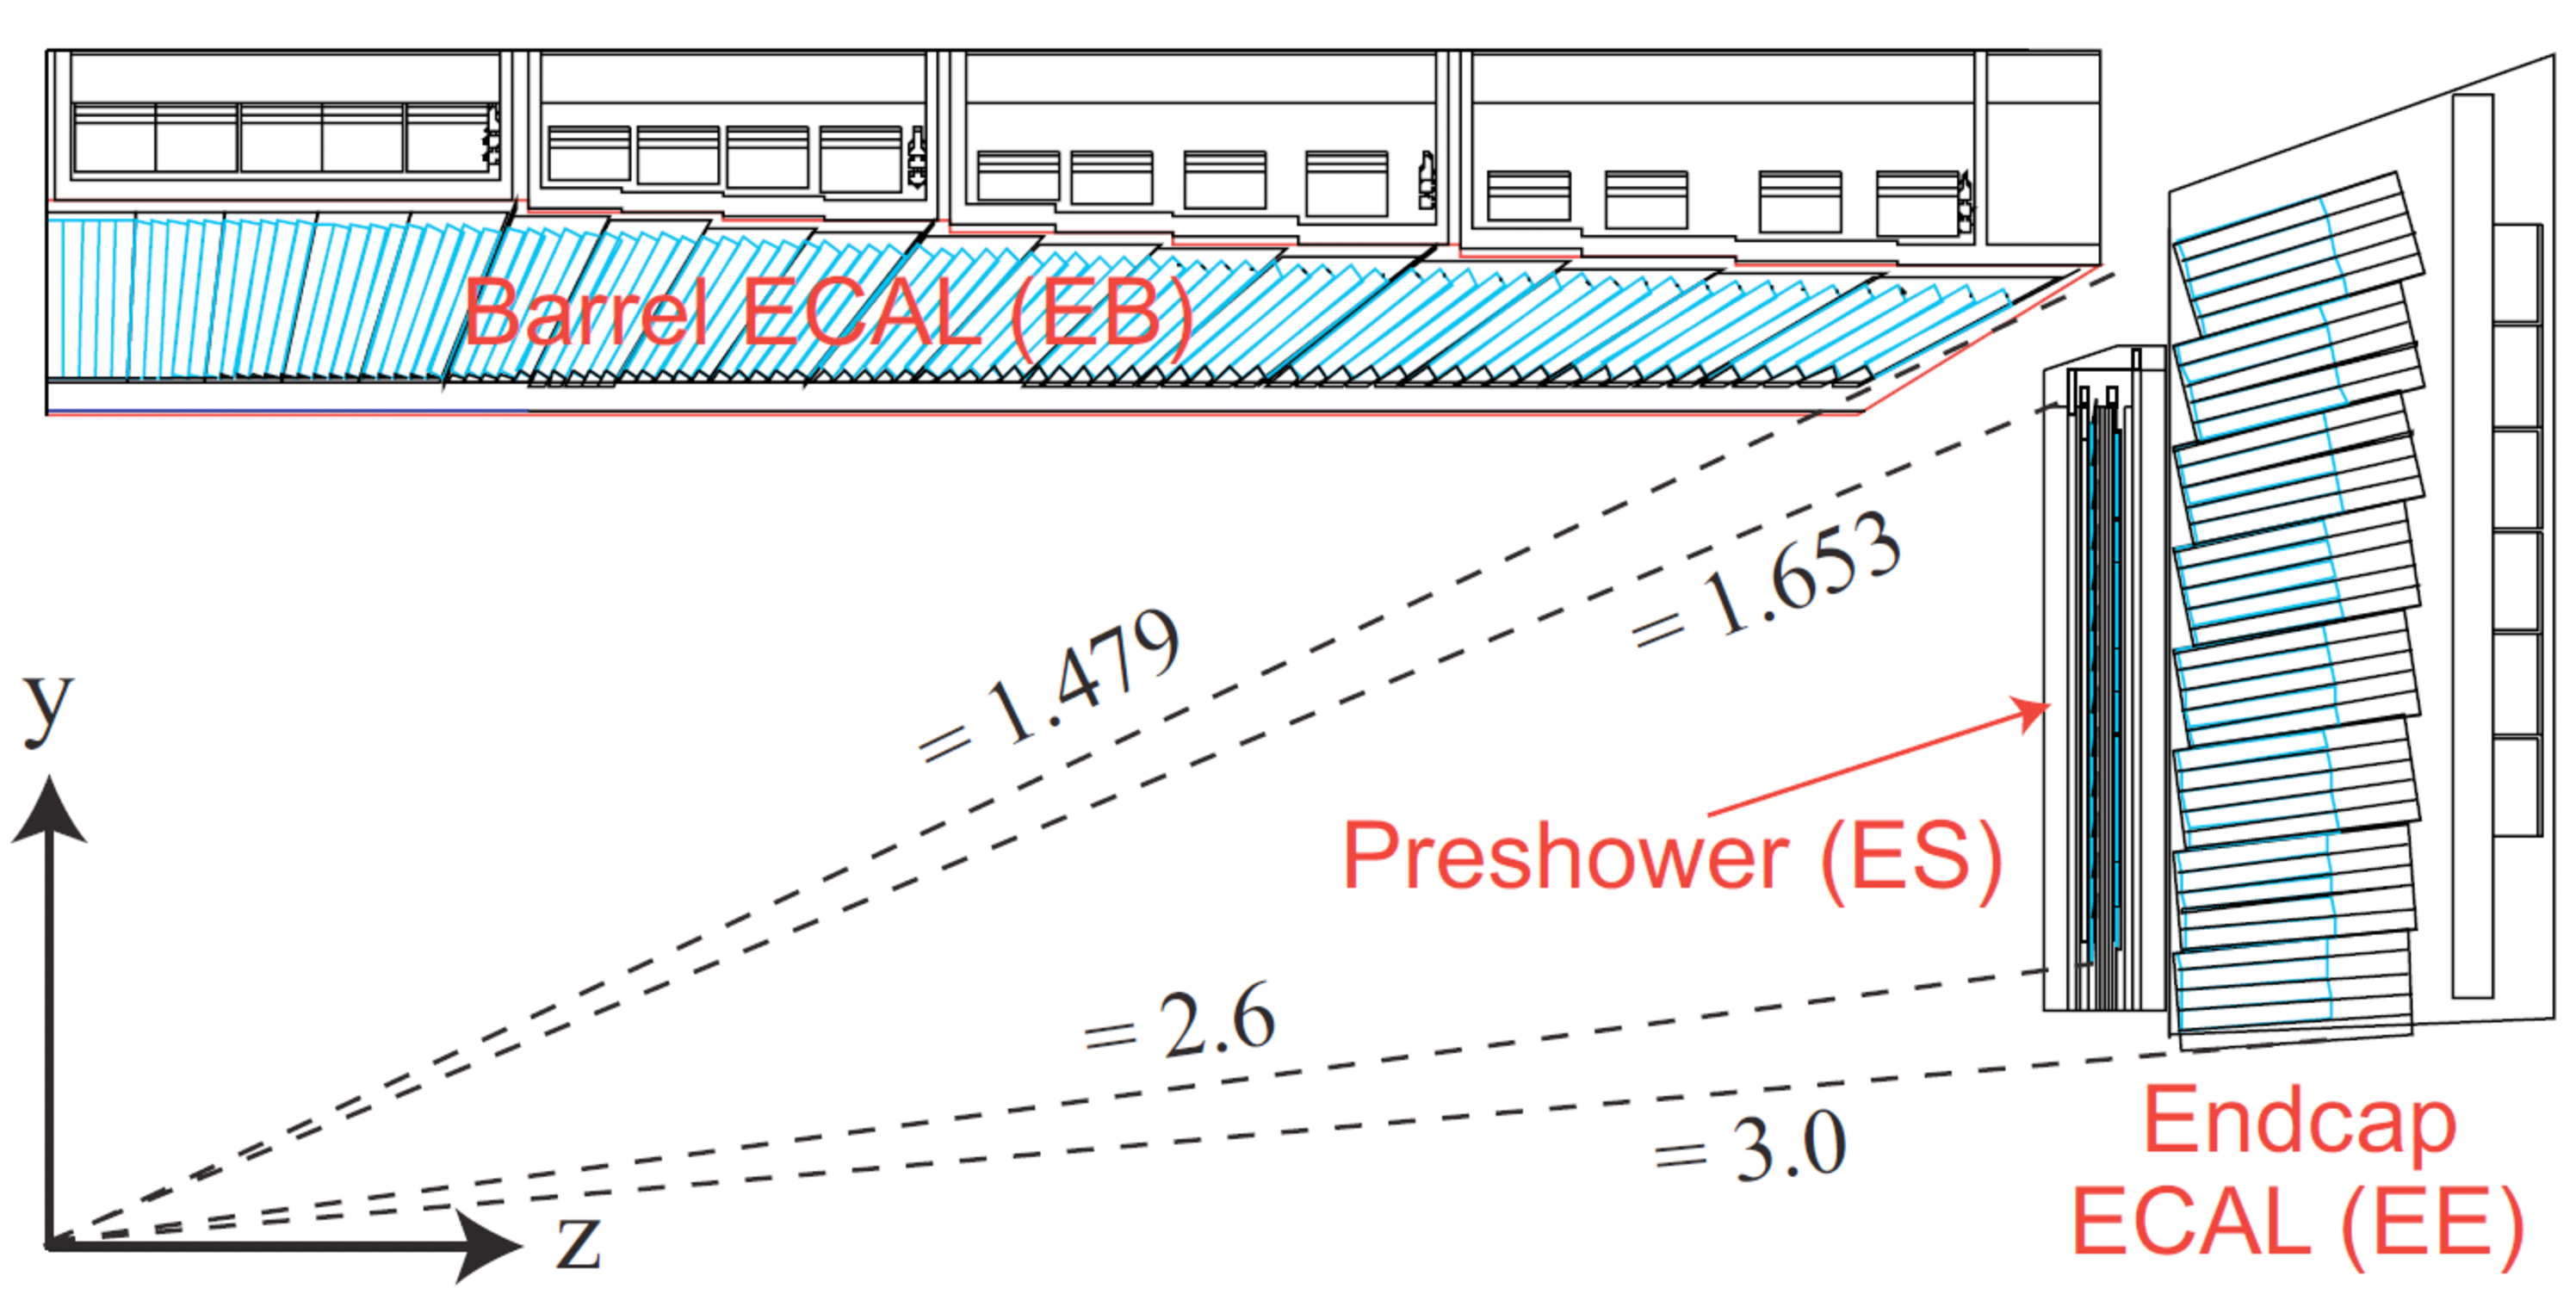
\includegraphics[width=0.9\textwidth]{ch3_figs/ecal_rapidity.pdf}
   \caption[Longitudinal view of the CMS ECAL]{Longitudinal view of one quarter of the ECAL~\cite{cms_bluebook}.}
   \label{fig:cms_ecal}
 \end{center}
\end{figure}

\subsection{HCAL}
The CMS Hadronic Calorimeter (HCAL) measures the energy of hadrons via their strong force interaction with the detector material. The HCAL is situated outside the ECAL.
The HCAL is a sampling calorimeter made up of alternating layers of brass absorber and plastic scintillator material in four separate sections. The HCAL provides energy resolution that helps reconstruct and tag hadronic
particle decays, as well as reconstructing the $missing$ $transverse$ $energy$ or \met, which can be interpreted as the presence of neutrinos\footnote{The \met reconstruction actually occurs later, but the HCAL information
provides some of the necessary quantities}. Within each plastic scintillator tile are optical wavelength-shifting fibers.
Measuring less than 1 mm in diameter, these fibers connect to other optical fibers which send the light signals to Hybrid Photodiodes (HPDs) for readout. The fast and radiation-resistant HPDs amplify the light and convert it
into an electronic signal via the photoelectric effect.

\begin{figure}[hbtp]
 \begin{center}
   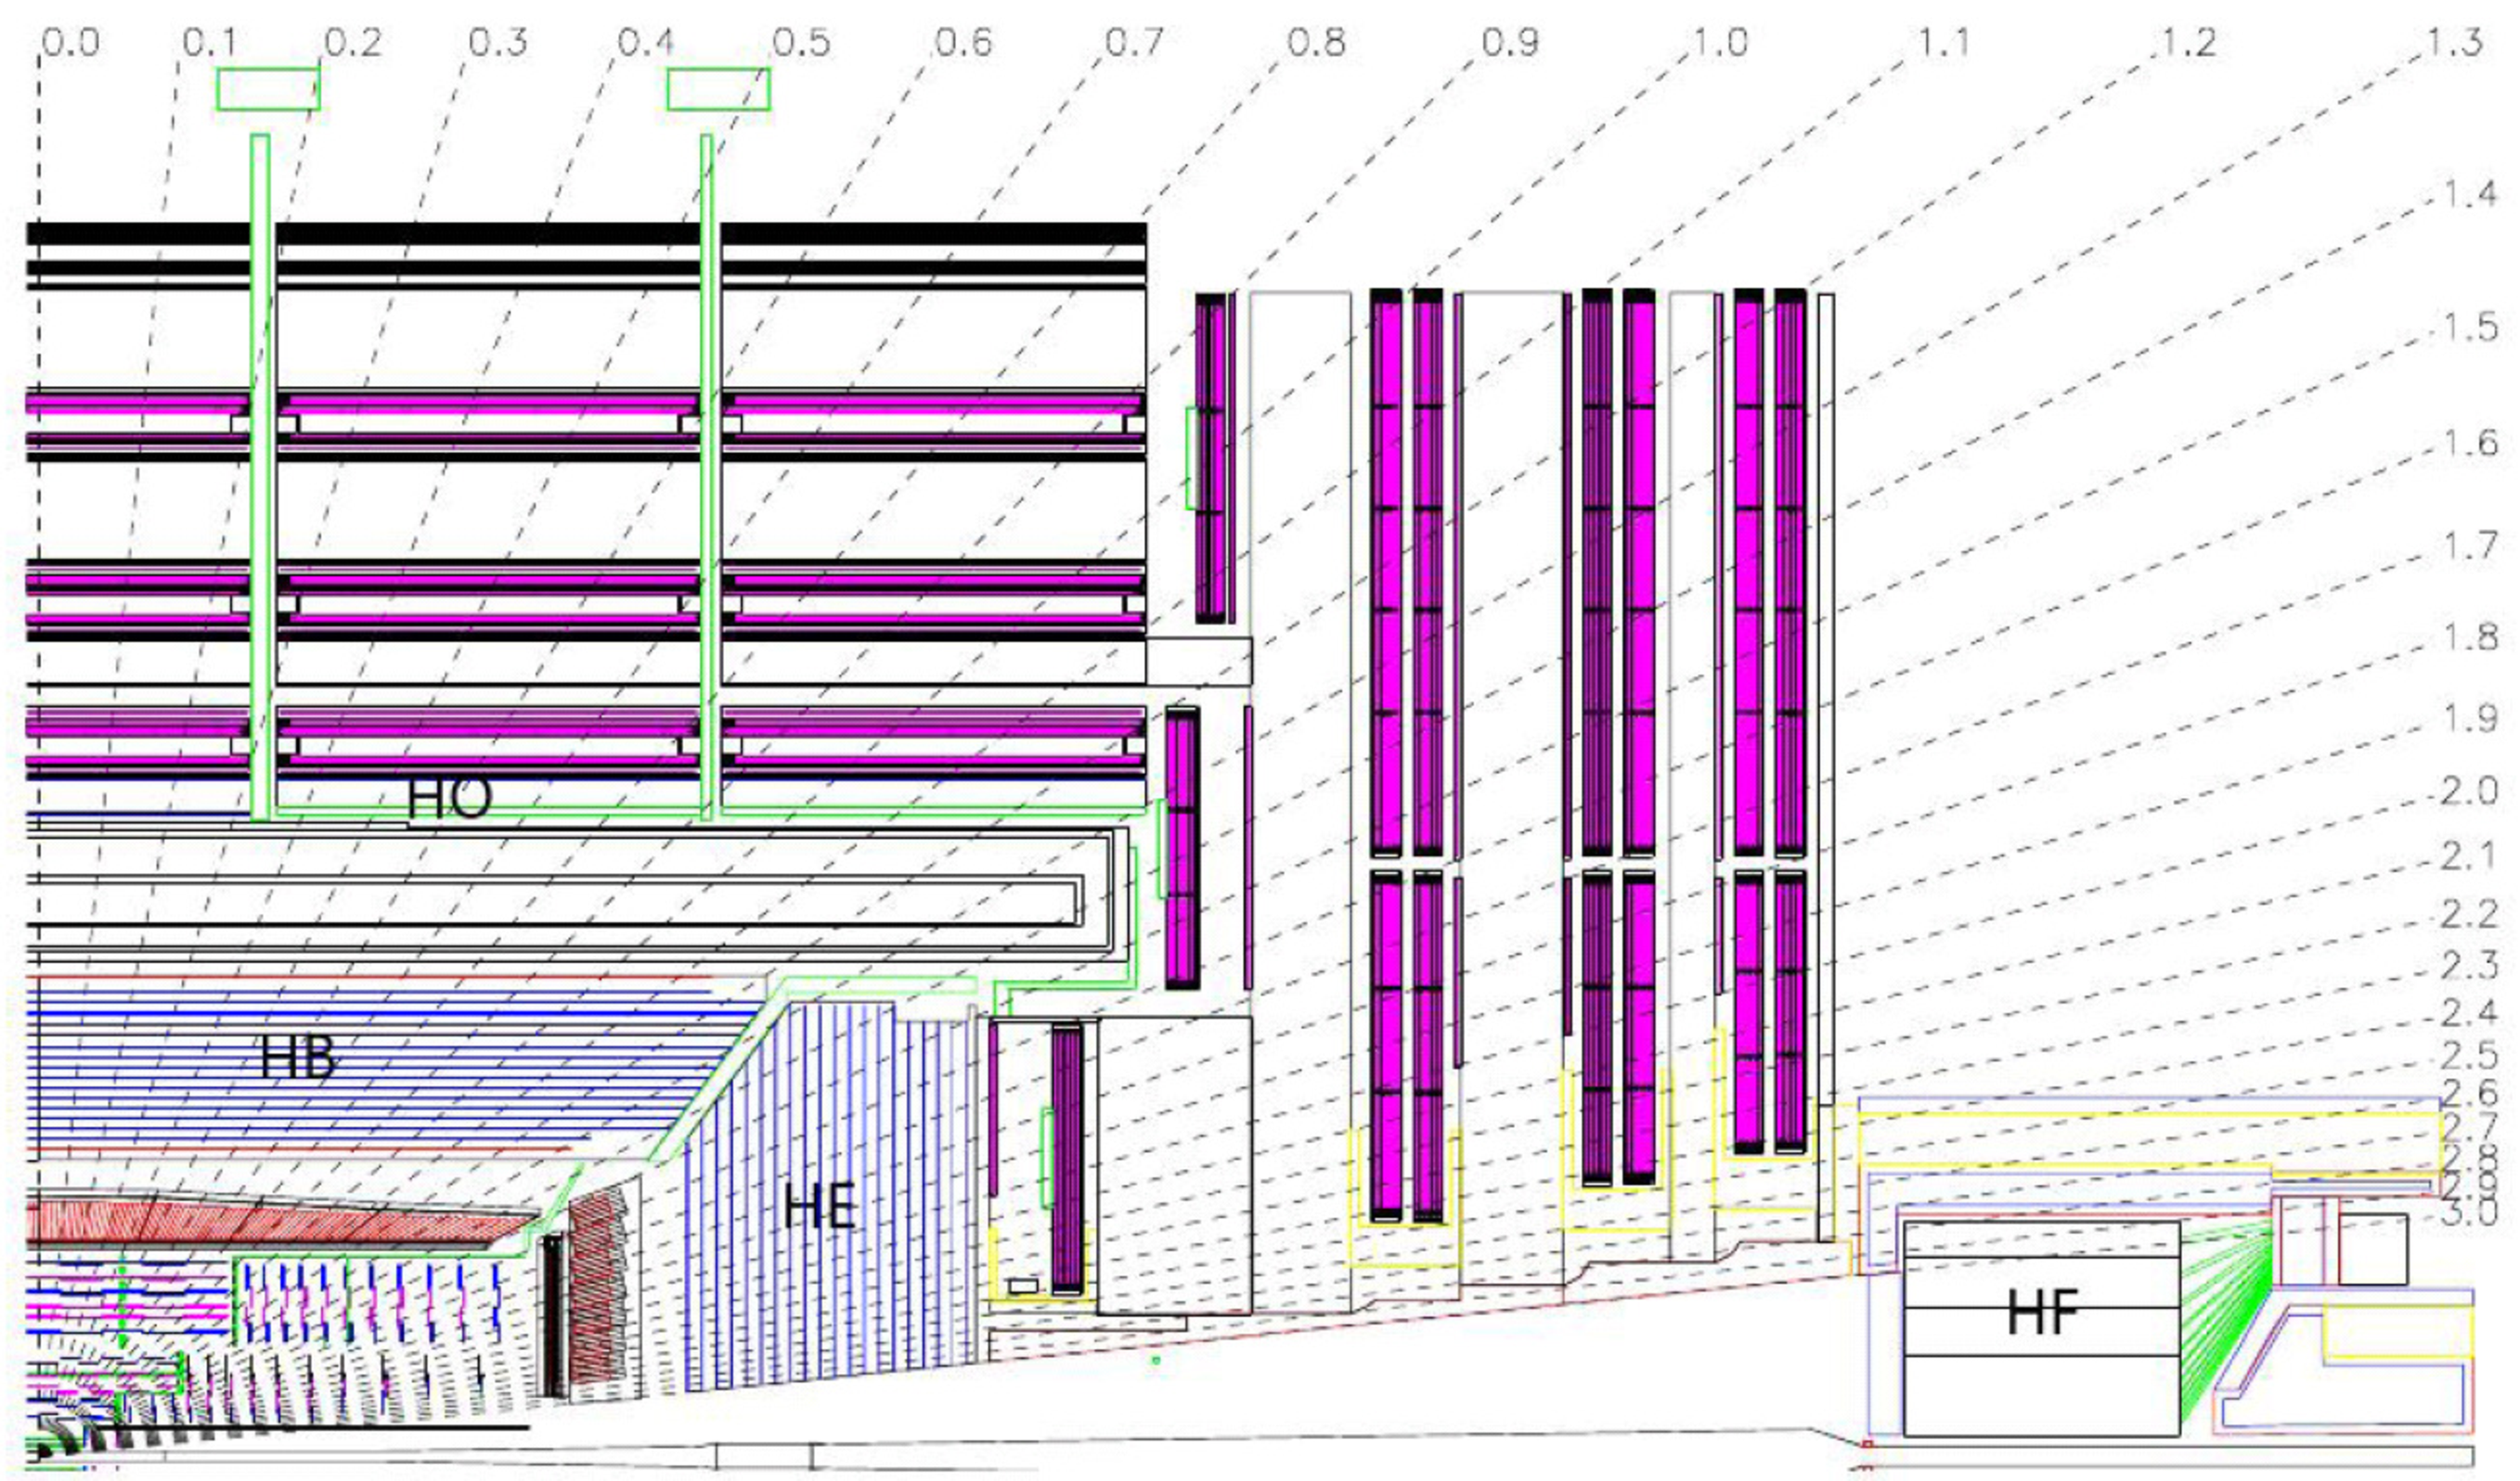
\includegraphics[width=0.9\textwidth]{ch3_figs/hcal.pdf}
   \caption[Longitudinal view of the CMS HCAL]{Longitudinal view of one quarter of the HCAL~\cite{cms_bluebook}.}
   \label{fig:cms_hcal}
 \end{center}
\end{figure}

As strongly-interacting particles travel through the HCAL, they interact with the dense brass absorber material decaying and producing showers of secondary particles which further cascade and travel through the scintillator and absorber material.
As the shower particles pass through the scintillator material, they emit a blue-violet light. This blue-violet light is then converted to green light via the wavelength shifting fibers and sent to the HPDs for readout. Like the ECAL,
the amount of light emitted corresponds to the amount of energy deposited. 

The four sections of the HCAL are the barrel (HB), the endcaps (HE), the outer barrel (HO) and the forward HCAL (HF) in Figure~\ref{fig:cms_hcal}. The barrel extends from 1.77 m to 2.95 m from the interaction point and
sits between the outside of the ECAL barrel and the inside of the magnet coil in the transverse plane. The HB covers a pseudorapidity range of $|\eta| < 1.3$.
The endcaps cover a pseudorapidity of $1.3 < |\eta| < 3$. The HO sits outside and around the solenoid coil covering the same pseudorapidity range
as the HB. The HO utilizes the magnet coil as an additional absorbing layer ensuring detection of any particle exiting the HB. The HF sits outside of all other subdetectors at $\pm$11 m from the interaction point in the z-direction,
covering a pseudorapidity range of $3.0 < |\eta| < 5.0$. The HF was specially designed to resist the intense radiation deposited in this forward region. In total, the endcap calorimeters cover roughly 10 radiation lengths.

\subsection{Solenoid}
Central to the design and name of CMS, the CMS magnet is one of the largest superconducting solenoids in the world.
At 12 m in length, it produces a field of nearly 3.8 T inside the 6 m diameter free bore, with the flux returned through a 10000 ton iron yoke.
The magnetic field outside the free bore in the muon chambers is approximately 2 T.  
Similar to the LHC magnets, the solenoid uses NbTi coils cooled to 1.8 K but carries a current of over 19000 amps. When fully energized, the magnet
stores 2.6 GJ of energy, enough to power 24 American homes for 1 day\cite{magnet_energy}. The central barrel of the solenoid sits between the HCAL and the muon chambers, with the return yoke interwoven with the muon chambers.

A strong magnetic field is essential for measuring the momentum of charged particles. Charged particles moving relativistically in a magnetic field are subject to the Lorentz force, described in
equation~\ref{eqn:lorentz_force} 

\begin{equation}
\label{eqn:lorentz_force}
 \vec{F} = \gamma q\vec{v} \times \vec{B}
\end{equation}

The solenoid produces a magnetic field along the z-direction and by the right-hand-rule from the cross product in equation~\ref{eqn:lorentz_force}, this means the particles experience a centripetal force, which
curves or deflects their trajectories. By setting the Lorentz force equal to the relativistic centripetal force in equation~\ref{eqn:lorentz_qvb}, the momentum and charge of the particle can be found by measuring the radius of the track. 
Thus the field produced by the CMS solenoid together with accurate track reconstruction, allows for precise momentum measurements of the particles.

\begin{equation}
\label{eqn:lorentz_qvb}
 \gamma qvB = \frac{m\gamma^{2}v^{2}}{r}
\end{equation}

\subsection{Muon Chambers}
A central feature of CMS, the muon chambers are solely dedicated to detecting and measuring muons.
Muons are not stopped by the ECAL due to their large mass, and travel through the HCAL and solenoid yoke mostly unimpeded since they don't interact via the strong force.
The muon chambers are the outermost subdetector for this reason. The muon chambers are comprised of 3 unique gas detection systems consisting of Drift Tubes (DTs),
Cathode Strip Chambers (CSCs), and Resistive Plate Chambers (RPCs), which each serve a specific purpose. Each of the gas chambers produce voltage pulses as muons pass through and leave hits.
Similar to the tracker, the hits are reconstructed into muon tracks, which can then be used to determine the momentum of the muon in the magnetic field.  

\begin{figure}[hbtp]
 \begin{center}
   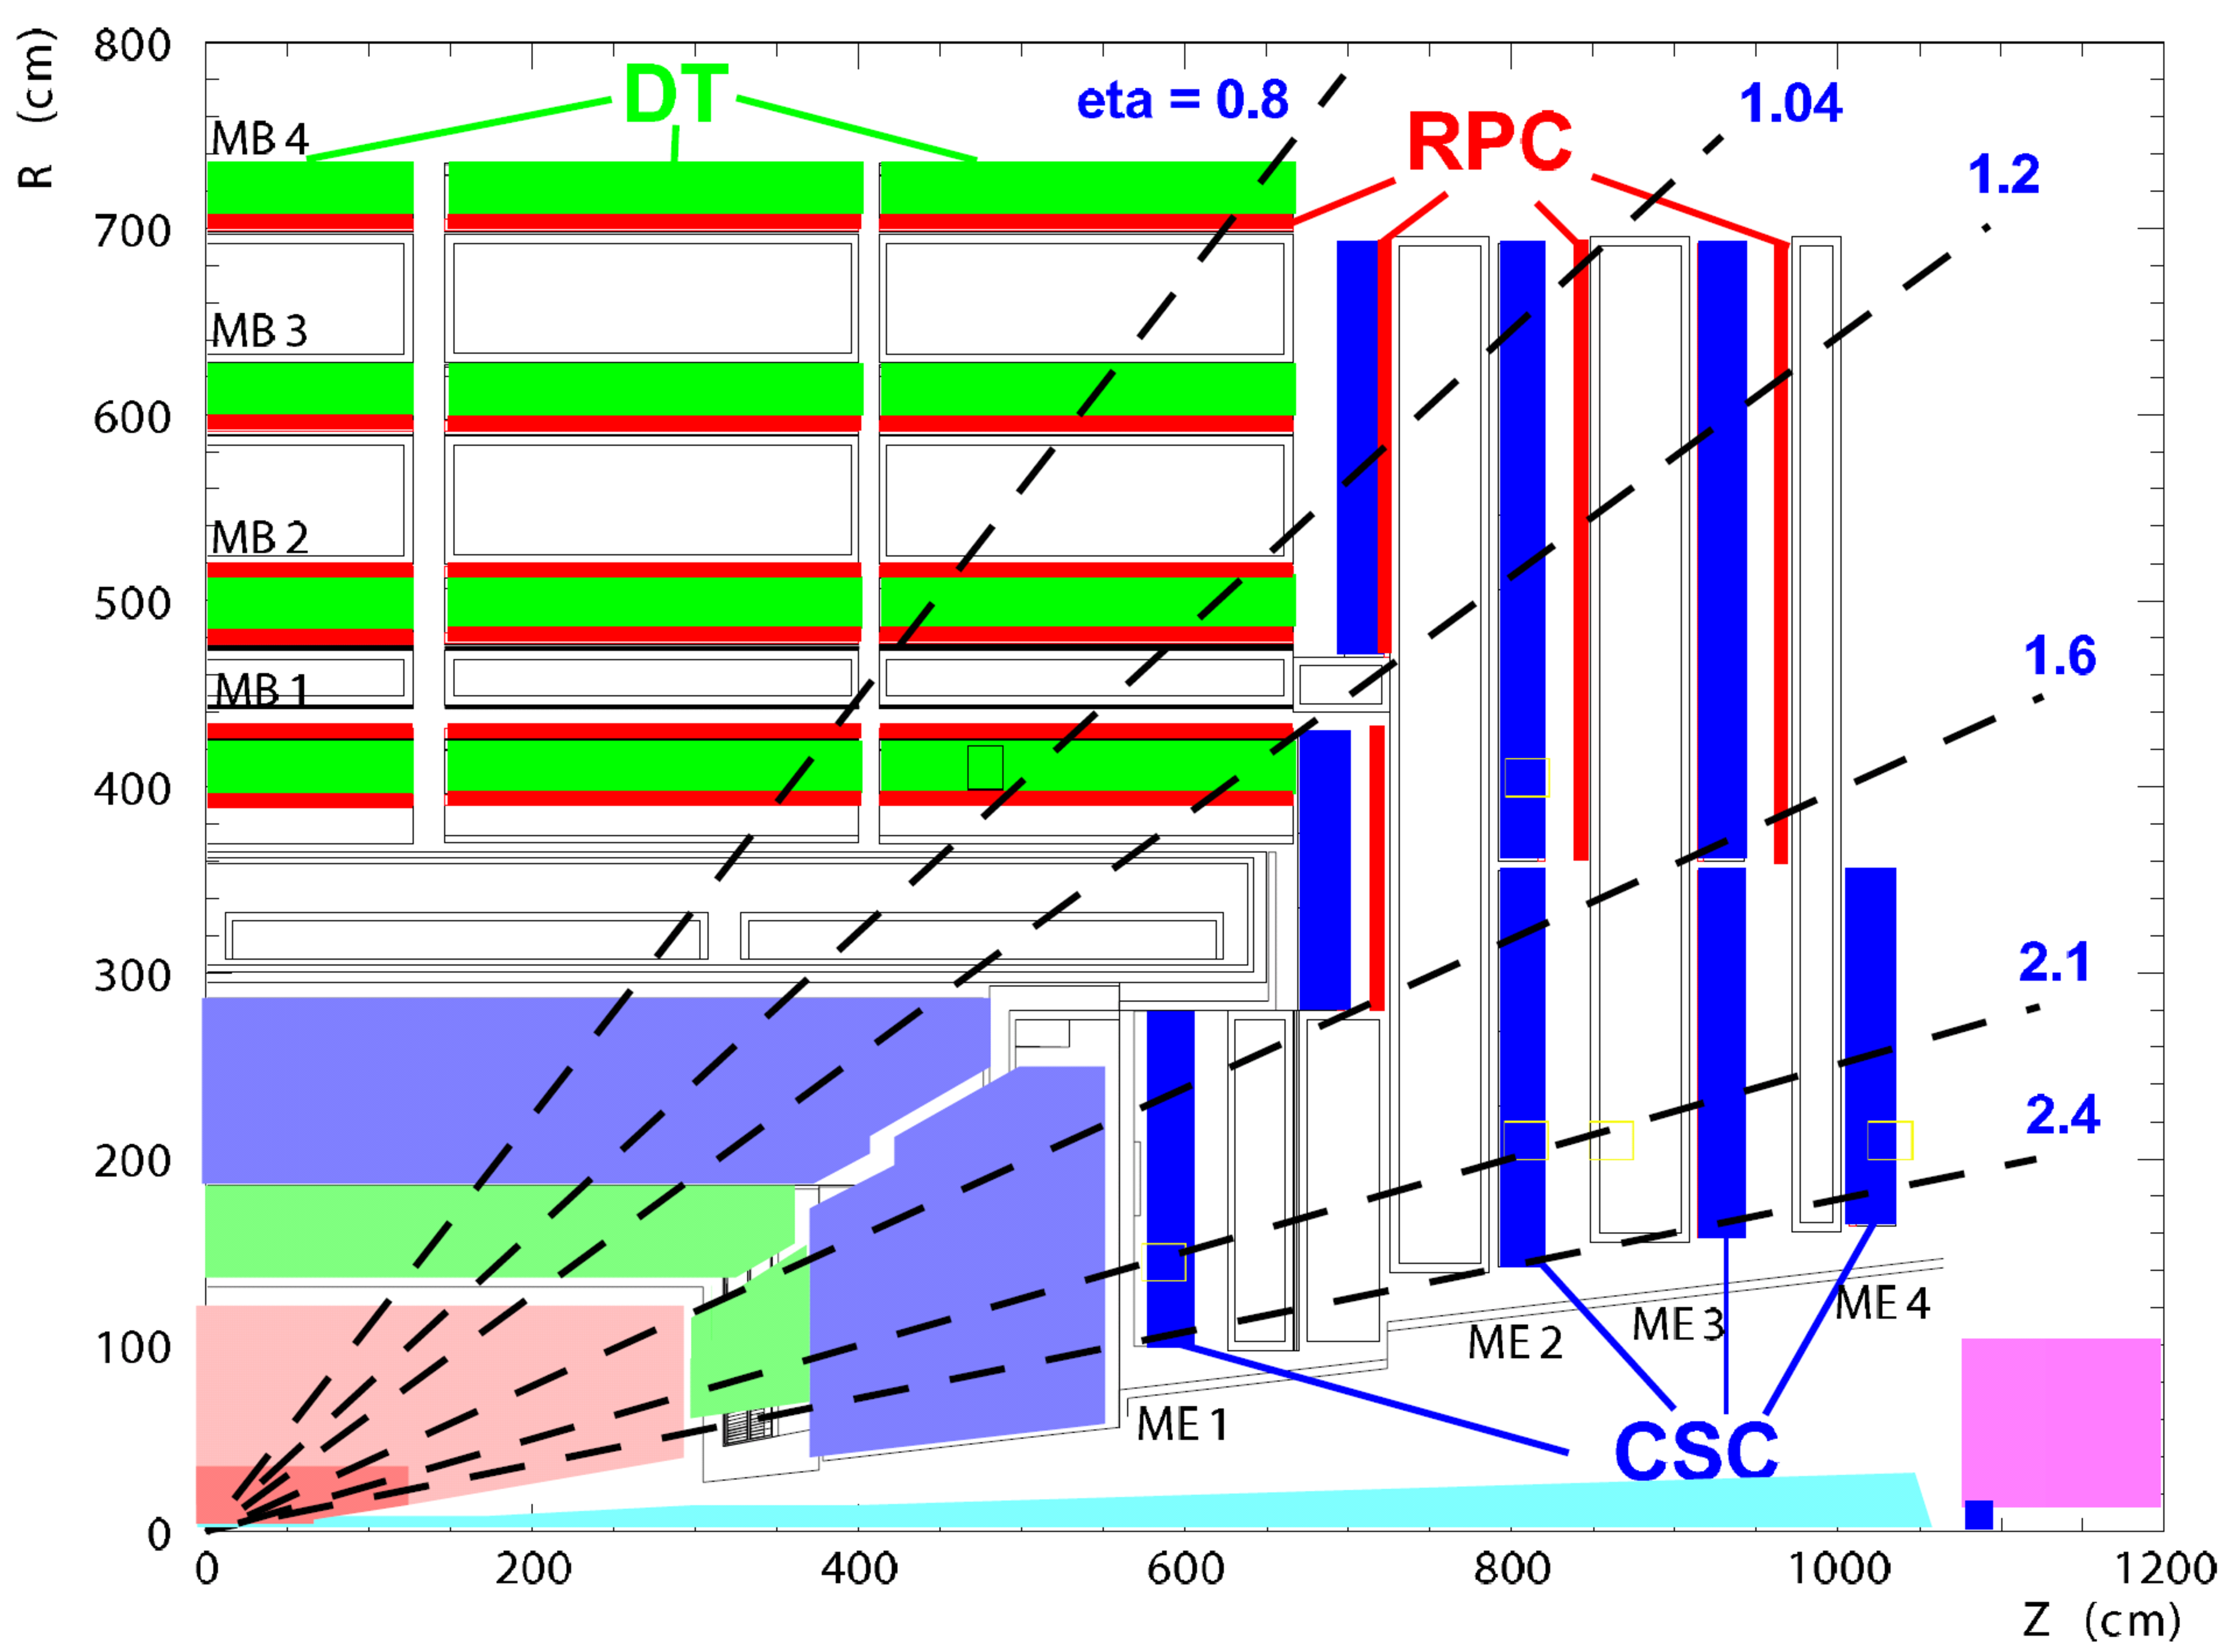
\includegraphics[width=0.9\textwidth]{ch3_figs/cms_muonchamber.pdf}
   \caption[Longitudinal view of the CMS muon chambers]{Longitudinal view of one quarter of the CMS muon chambers~\cite{cms_bluebook}.}
   \label{fig:cms_muonchamber}
 \end{center}
\end{figure}

The DTs cover the barrel region of the detector. There are three concentric cylindrical layers each containing 60 drift tube chambers and one additional outer layer with 70.
Each drift tube is constructed from light weight aluminum and measures 4 cm wide by 2.4 m long, filled with a mixture of 85$\%$ Ar and 15$\%$ $CO_{2}$ gas.
Cathode strips held at -1.2 kV run the length of each cell with a gold-plated steel anode wire held at 3.6 kV runs down the center (see Figure~\ref{fig:cms_dt}).

As an incident muon ionizes the gas atoms, electrons are attracted to the anode wire while positively charged ions are attracted to the cathodes. 
The ions induce a current fluctuation in the electrodes which is readout and interpreted as a hit. By knowing the drift velocities of ions in the gas and measuring
the timing of the current pulses precisely, the position of the muon from the anode wire is inferred. By alternating the orientation of these chambers between wires parallel to the beamline
and wires perpendicular to the beamline, the DTs can resolve muon positions to 100 $\mu$m. 
The DTs are used in the barrel only, where there are lower particle fluxes and intensities. 

\begin{figure}[hbtp]
 \begin{center}
   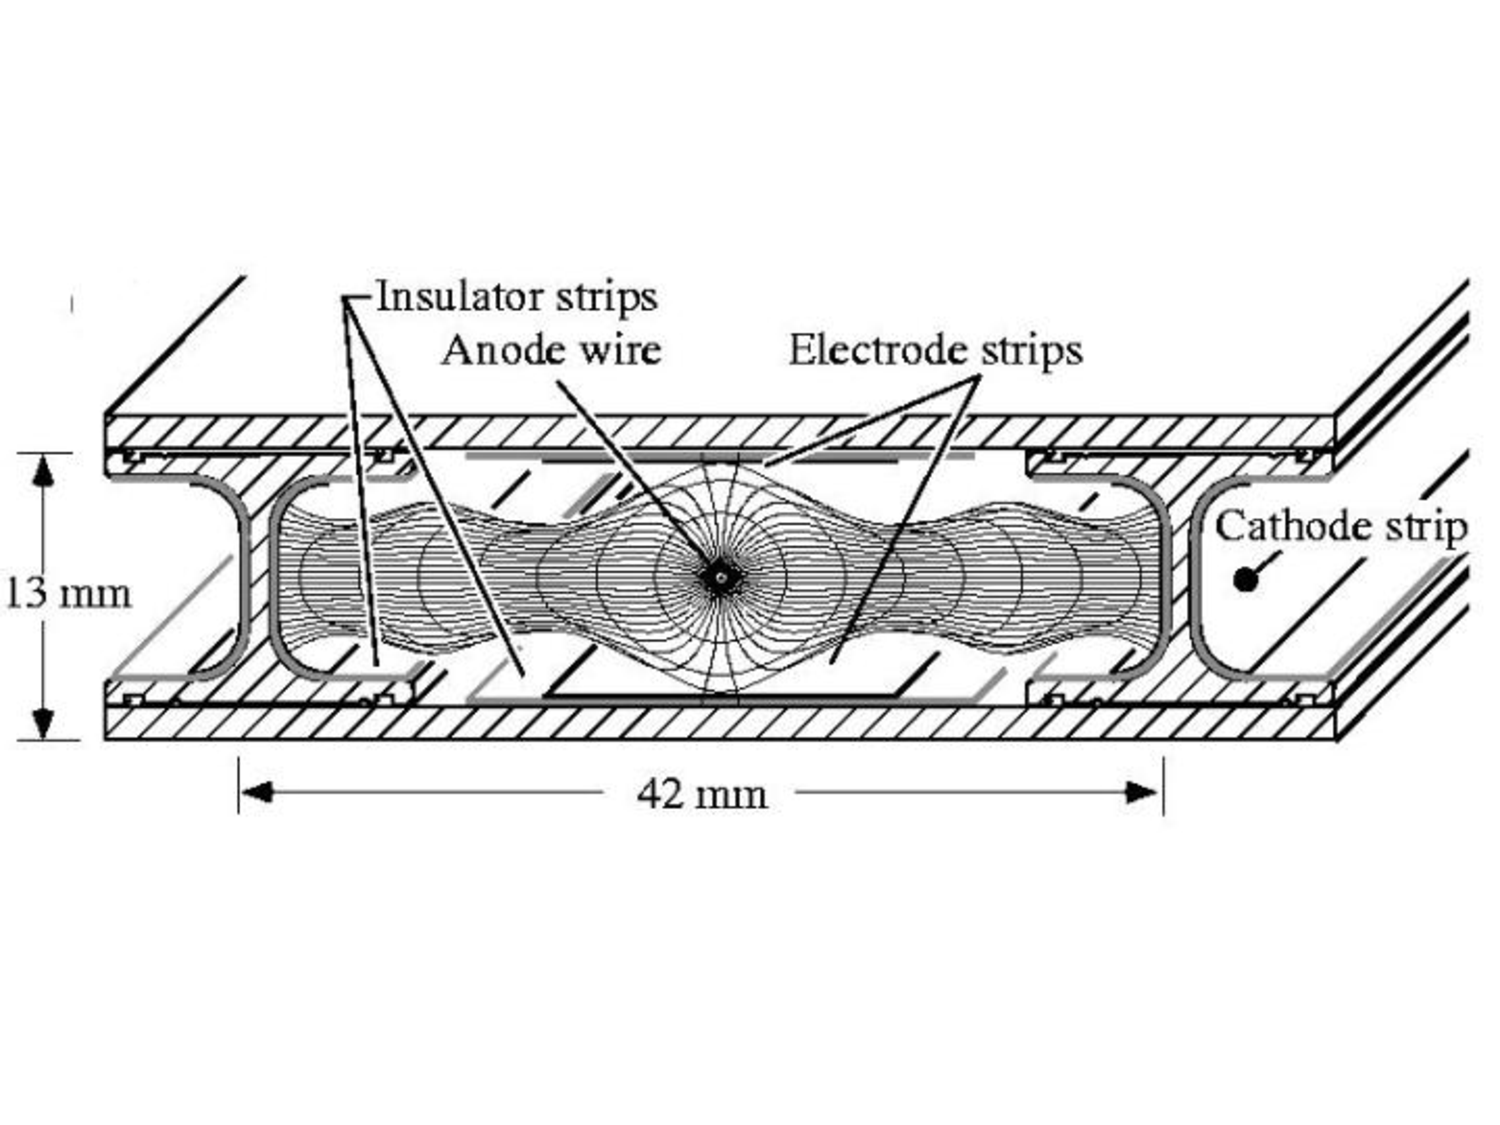
\includegraphics[width=0.9\textwidth]{ch3_figs/cms_dt.pdf}
   \caption[Drift tube chamber and internal E field]{A map of the electric field of the drift tubes in absence of magnetic field~\cite{cms_bluebook}.}
   \label{fig:cms_dt}
 \end{center}
\end{figure}

The CSCs are used only in the endcaps, where there is a greater particle intensity and because the large, non-uniform magnetic field would affect the ion drift of DTs - making them unsuitable in this region.
468 CSCs in 7 layers are in the endcaps, where each chamber is trapezoidal in shape.
Each chamber consists of positively charged anode wires which cross negatively charged cathode strips that are enclosed in a chamber filled with gas. As muons enter a
CSC, they ionize the gas causing freed electrons to travel to the positive wires and positive charges migrate towards the cathode strips. The charge pulses are detected in both the strips
and the wires, which are perpendicular to each other, providing two coordinates for each muon hit. The CSCs provide good position information quickly, making them suitable for use in the endcaps. 

\begin{figure}[hbtp]
 \begin{center}
   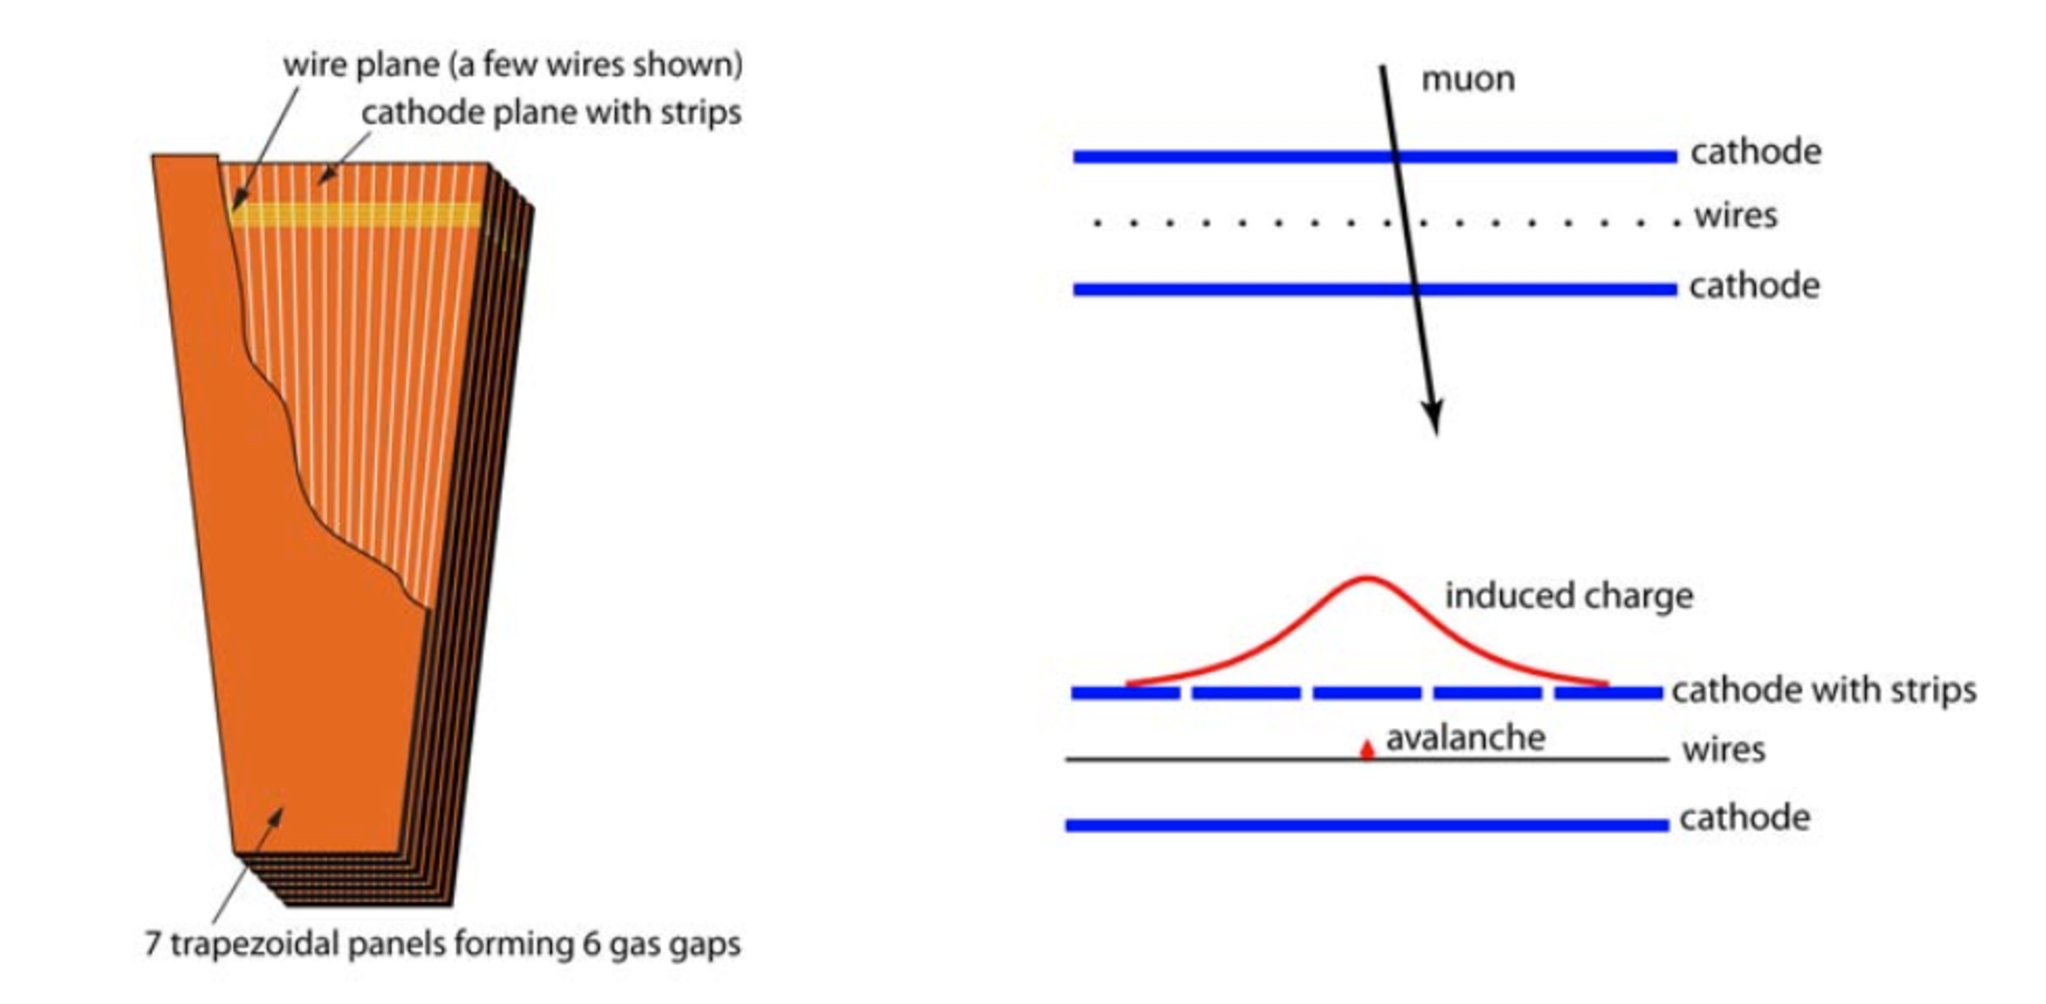
\includegraphics[width=0.9\textwidth]{ch3_figs/cms_csc.pdf}
   \caption[CSC module and operation schematic]{CSC module (left) and a depiction of the CSC operation (right). The strips provide precise position information~\cite{cms_bluebook}.}
   \label{fig:cms_csc}
 \end{center}
\end{figure}

The third type of muon detector used is the RPC. The RPCs are used in both the barrel and the endcaps covering out to $|\eta| < 1.6$,
providing redundant coverage. The RPCs are characterized by their fast response time which makes them suitable for triggering, unlike the DTs and CSCs, which 
are limited by their relatively longer drift times.
Due to this very fast response time ($\<$ 1 ns), the RPCs easily identify which bunch crossing a detected muon is associated with, since the bunch time spacing is 25ns.  
The RPCs are gaseous parallel plate detectors. Each RPC measures between 2.1-2.5 m in length and 1.5-2.5 m wide, with a thickness of 2mm filled with gas separating
two resistive plastic parallel plates, an anode and cathode.
As an incident muon ionizes the gas atoms releasing electrons, the electrons in turn ionize nearby gas atoms resulting in an avalanche of electrons which drift towards the anode
and are picked up by metallic detecting strips. The hit pattern on the strips is used to determine the muon momentum for fast trigger decisions.

\begin{figure}[hbtp]
 \begin{center}
   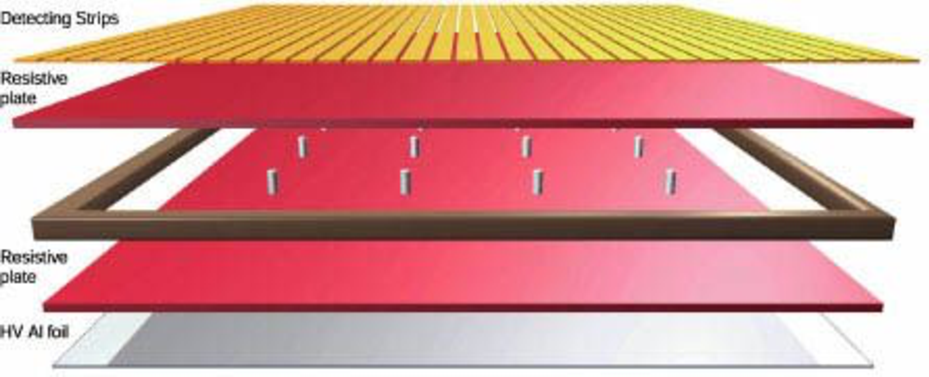
\includegraphics[width=0.9\textwidth]{ch3_figs/cms_rpc.pdf}
   \caption[CMS RPC diagram]{A qualitative depiction of an RPC~\cite{cms_bluebook}.}
   \label{fig:cms_rpc}
 \end{center}
\end{figure}
 
\subsection{Trigger and Data Acquisition}

The LHC collides proton bunches at a frequency of almost 35 MHz, making efficient data collection and filtering necessary. This task is accomplished with the trigger and Data Acquisition system (DAQ). Because not all collisions can be recorded,
and most collisons don't produce events that warrant further analysis, the trigger ``fires'' on interesting events only, and sends the information readout in each subdetector to the DAQ. The CMS trigger is comprised of two parts or levels.
The Level 1 (L1) is the frontline of the CMS trigger system, comprised of firmware and basic software that is directly connected to each subdetector's readout electronics. The second part of the trigger is called the High Level Trigger (HLT)
and is entirely software-based, running a filter farm of high-performance CPUs. 

The L1 is the first place where an event can be discarded or selected based on predefined conditions. From an event rate of 40 MHz produced by the LHC, the L1 filters and reduces this to between 80-100 kHz.  
Each subdetector readout, with the exception of the silicon trackers, is directly connected to the L1. Since the trackers have very high occupancies, and millions
of pixels and strips, sophisticated track reconstruction takes much longer than is acceptable for a L1 trigger decision. Therefore when the L1 fires based on other subdetector information, the tracker is immediately readout and the information is saved
but not reconstructed. The software portion of the L1 consists of 128 algorithms called triggers or bits, that are constantly processing detector readout information. Any one trigger accepting an event, will pass all the detector information downstream
to the HLT. 

The HLT receives events that pass the L1, and is the final filter that determines which events are saved or discarded. This means that all events passing the HLT are saved and reconstructed for later analysis.
The HLT reduces the L1 input rate from 100 kHz to around 1 kHz. The HLT software is the foundation on which the rest of the offline CMS analysis software, CMSSW, is built. The HLT software consists of over 400 trigger algorithms that make accept/reject decisions
based on quantities such as particle momenta, multiplicity, energy, position, and other more sophisticated variables that are available thanks to the advanced event reconstruction that takes place at the HLT.
The more than 400 HLT algorithms (triggers) are gouped into categories based on the specific types of objects that fire the trigger such as electron/photons, muons, Jets/MET etc. These groups are called primary datasets and only events which passed a trigger
allocated to that primary dataset will be found in the associated dataset. Common examples of primary datasets include SingleEG, DoubleEG, SingleMu, DoubleMu, MuonEG etc. The events are then sent further downstream grouped together in these primary datasets.
The collection of 400 algorithms comprise the HLT menu.
Because the HLT, DAQ and downstream hardware can only handle a maximum trigger
rate, the trigger menu uses prescales to control the rates of triggers that would otherwise fire too often. This allows lower-priority triggers to collect data
without consuming large rates. The prescale controls the frequency of trigger accepts. For example a trigger with a prescale of 2 means that
data is recorded every other time the trigger fires.
The HLT and L1 algorithms are thoroughly tested and highly efficient at passing the objects they are
designed to accept. Typical HLT trigger efficiencies are well above 90$\%$. See the muon efficiency at the HLT in Figure~\ref{fig:hlt_eff_muons} below. 

\begin{figure}[hbtp]
 \begin{center}
   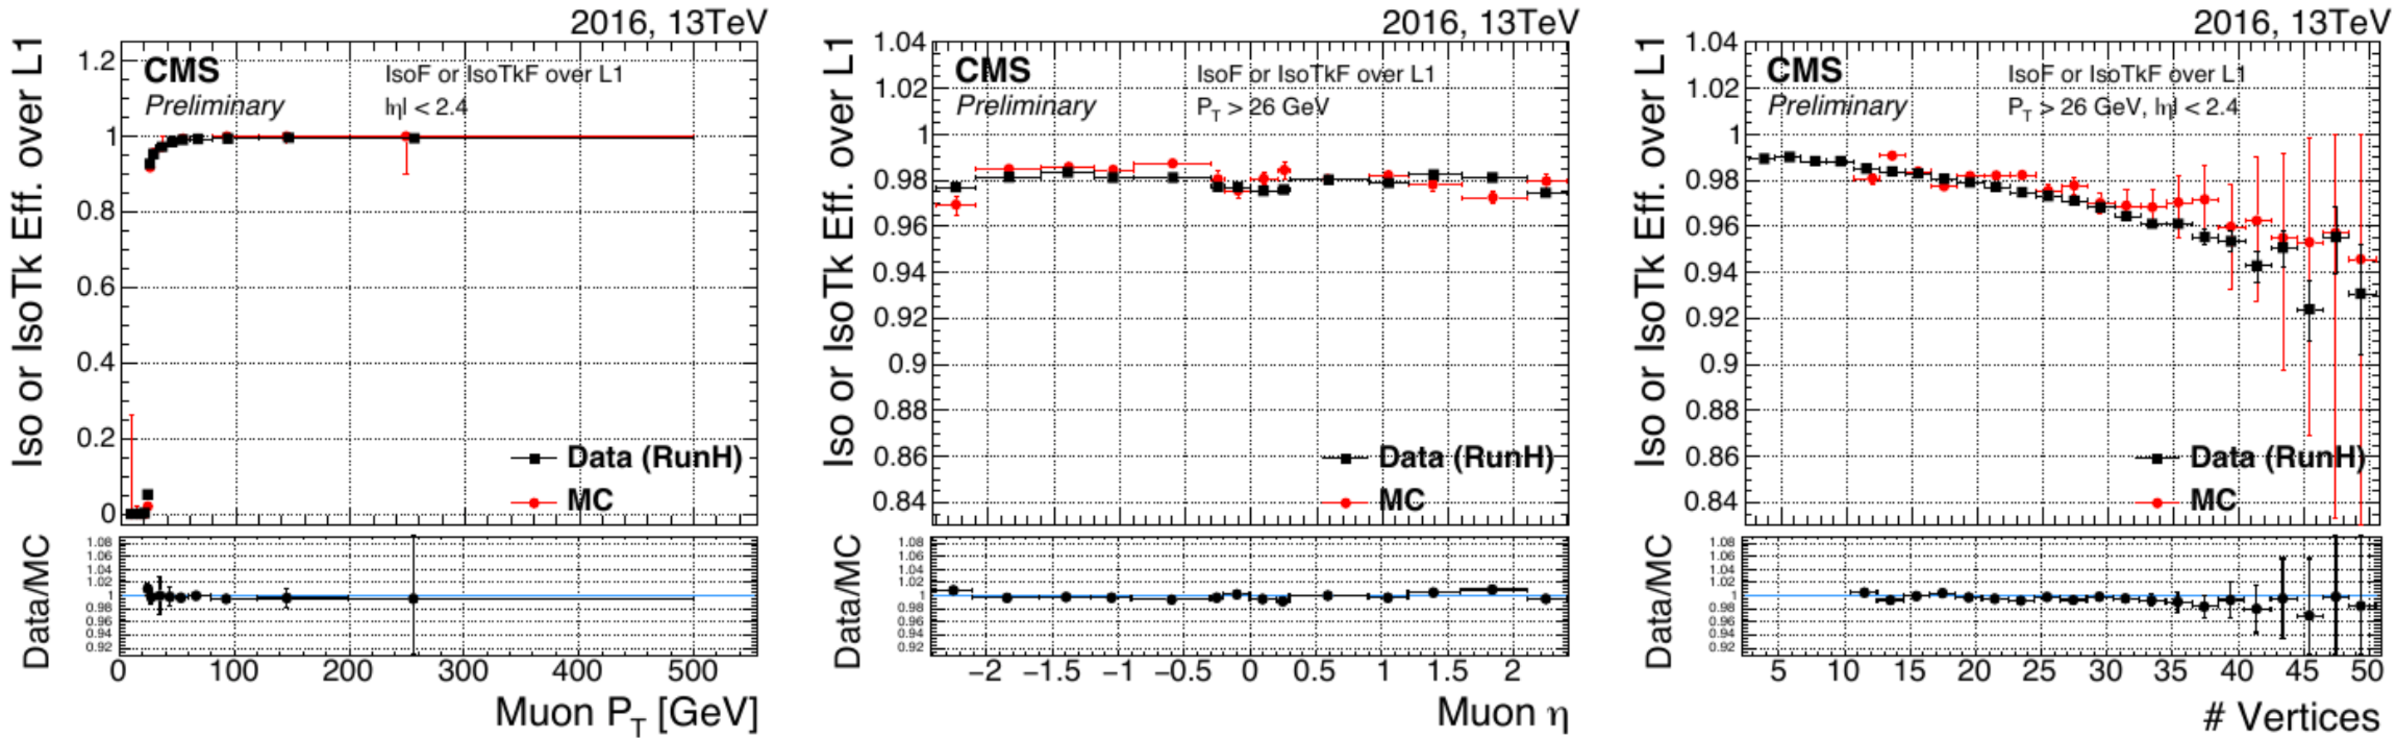
\includegraphics[width=0.9\textwidth]{ch3_figs/hlt_eff_muons.pdf}
   \caption[Trigger efficiency at the HLT]{Muon trigger efficiency at the HLT as a function of muon transverse momenta, pseudorapidity, and number of reconstructed vertices.}
   \label{fig:hlt_eff_muons}
   %%https://indico.cern.ch/event/512834/contributions/2349020/attachments/1370932/2079307/trigger.pdf
 \end{center}
\end{figure}

The CMS DAQ handles everything from the detector readout to interfacing the various parts of the L1 and HLT, as well as running the 1800+ CPU filter farm that the HLT software runs on. The DAQ also handles all data recorded by CMS,
sending it from the HLT
to an offsite computing facility for additonal reconstruction and distribution for analysis. The DAQ compiles information from the L1 and all subdetector readouts and synchronizes and combines this information together to build a complete picture of an
event before it even reaches the HLT.    

\begin{figure}[hbtp]
 \begin{center}
   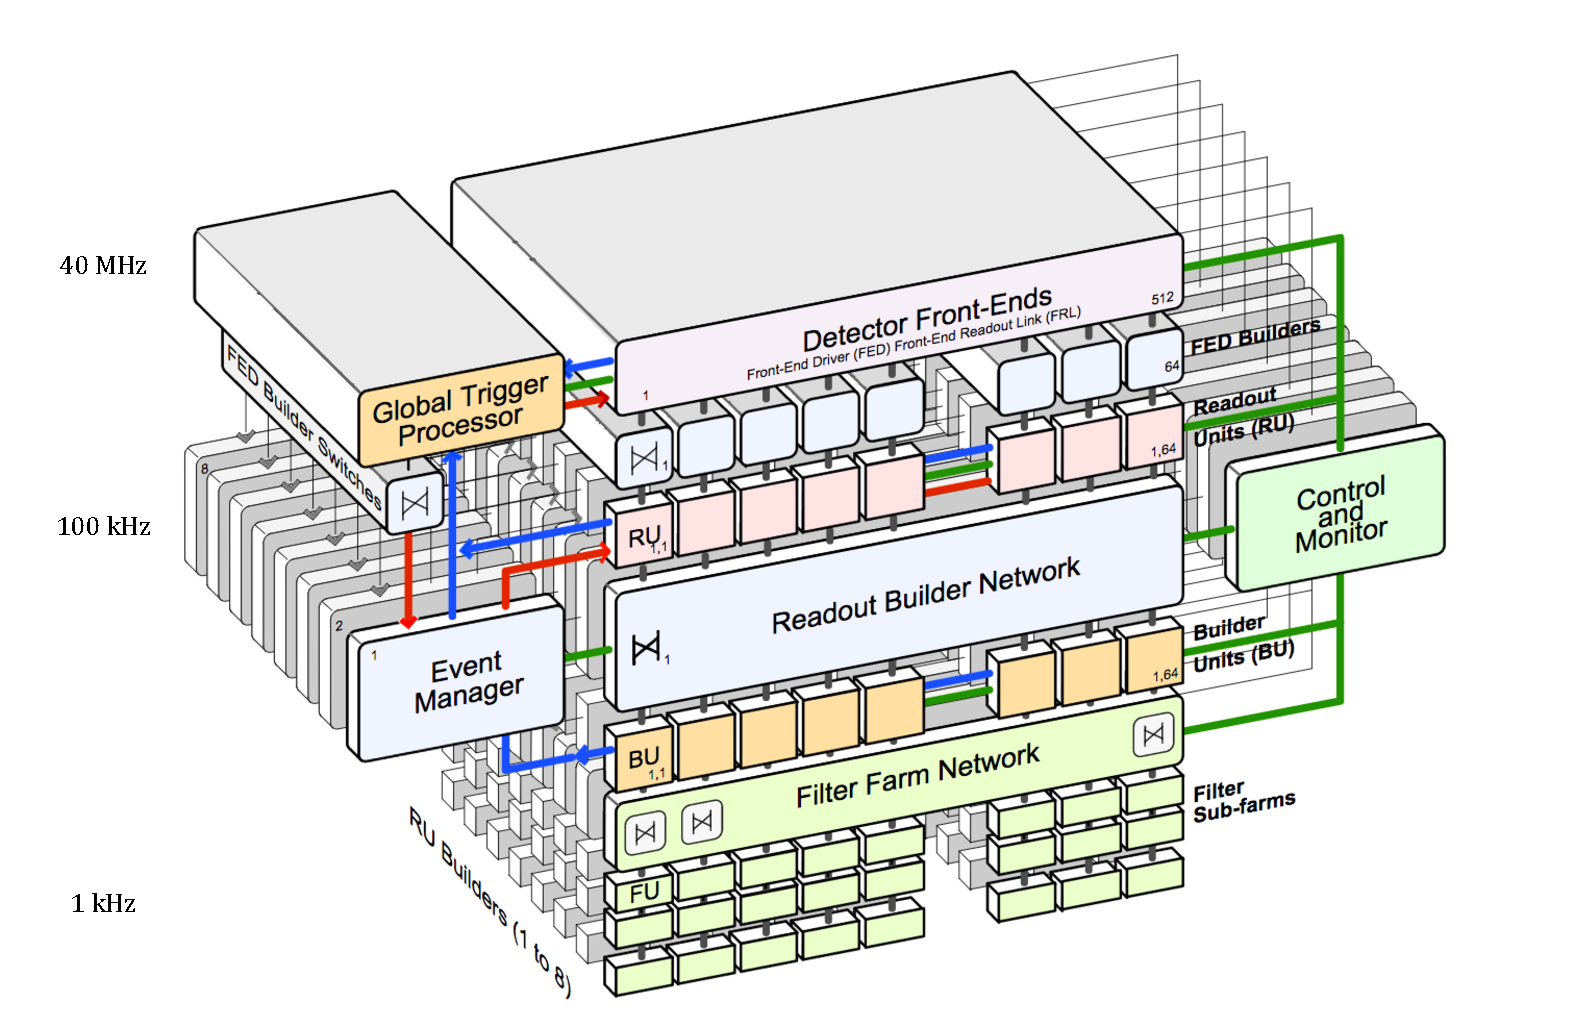
\includegraphics[width=0.9\textwidth]{ch3_figs/cms_daq.pdf}
   \caption[The CMS DAQ system]{A schematic of the DAQ system. After passing the L1, the events are built by combining all subdetector information into one coherent picture for the HLT (labeled Filter Farm Network) to make more sophisticated accept
     decisions~\cite{tridas}.}
   \label{fig:cms_daq}
   %%http://iopscience.iop.org/article/10.1088/1748-0221/3/08/S08004/pdf#%5B%7B%22num%22%3A215%2C%22gen%22%3A0%7D%2C%7B%22name%22%3A%22XYZ%22%7D%2C82.959%2C499.674%2Cnull%5D
 \end{center}
\end{figure}

% % uncomment the following lines,
% if using chapter-wise bibliography
%
% \bibliographystyle{ndnatbib}
% \bibliography{example}

%
% Chapter 4
%

\chapter{PHYSICS OBJECTS}
Each of the CMS subdetectors (neglecting the trigger system) technically only record and detect hits and energy deposits. While these hits and energy deposits are almost
always due to passing particles, the detectors themselves and more precisely the readouts, only produce information about the position, value, and multiplicity of
these hits and energy deposits. It is thanks to clever and accurate experimental techniques that we can reconstruct various particles from these hits and energy deposits.
In part because CMS does not detect particles directly, reconstructed particles are referred to as physics \emp{objects} in this context. Using
the term particles implies certainty about the identify of the object, and because there is some uncertainty, however small, inherent in the reconstruction, objects is
more accurate and widely used. The reconstruction technique varies greatly with different objects and the subdetectors used to detect and record their hits and energy
deposits. 

\section{Object Reconstruction and Particle Flow}
The particle flow algorithm is used by CMS to reconstruct physics objects from hits and energy deposits. Particle Flow and CMS are unique in the sense
that nearly all physics analyses performed on data collected by CMS use objects reconstructed with this single algorithm. The primary advantage of this strategy is
uniform and consistent object definitions across nearly all papers published on behalf of CMS. Other collaborations such as ATLAS do not use
the same algorithm collaboration-wide. The purpose of particle flow is to identify all final-state stable particles in an event recorded by CMS, specifically electrons,
mouons, taus, jets and photons. Particle flow optimally combines building-block information (hits and energy clusters) from all subdetectors to reconstruct objects and
determine particle type, position, and momentum. It does this using 2 different primary reconstruction techniques for reconstructing tracks from tracker hits, and clusters
of energy deposits from individual calorimeter cells. 

\begin{figure}[hbtp]
 \begin{center}
   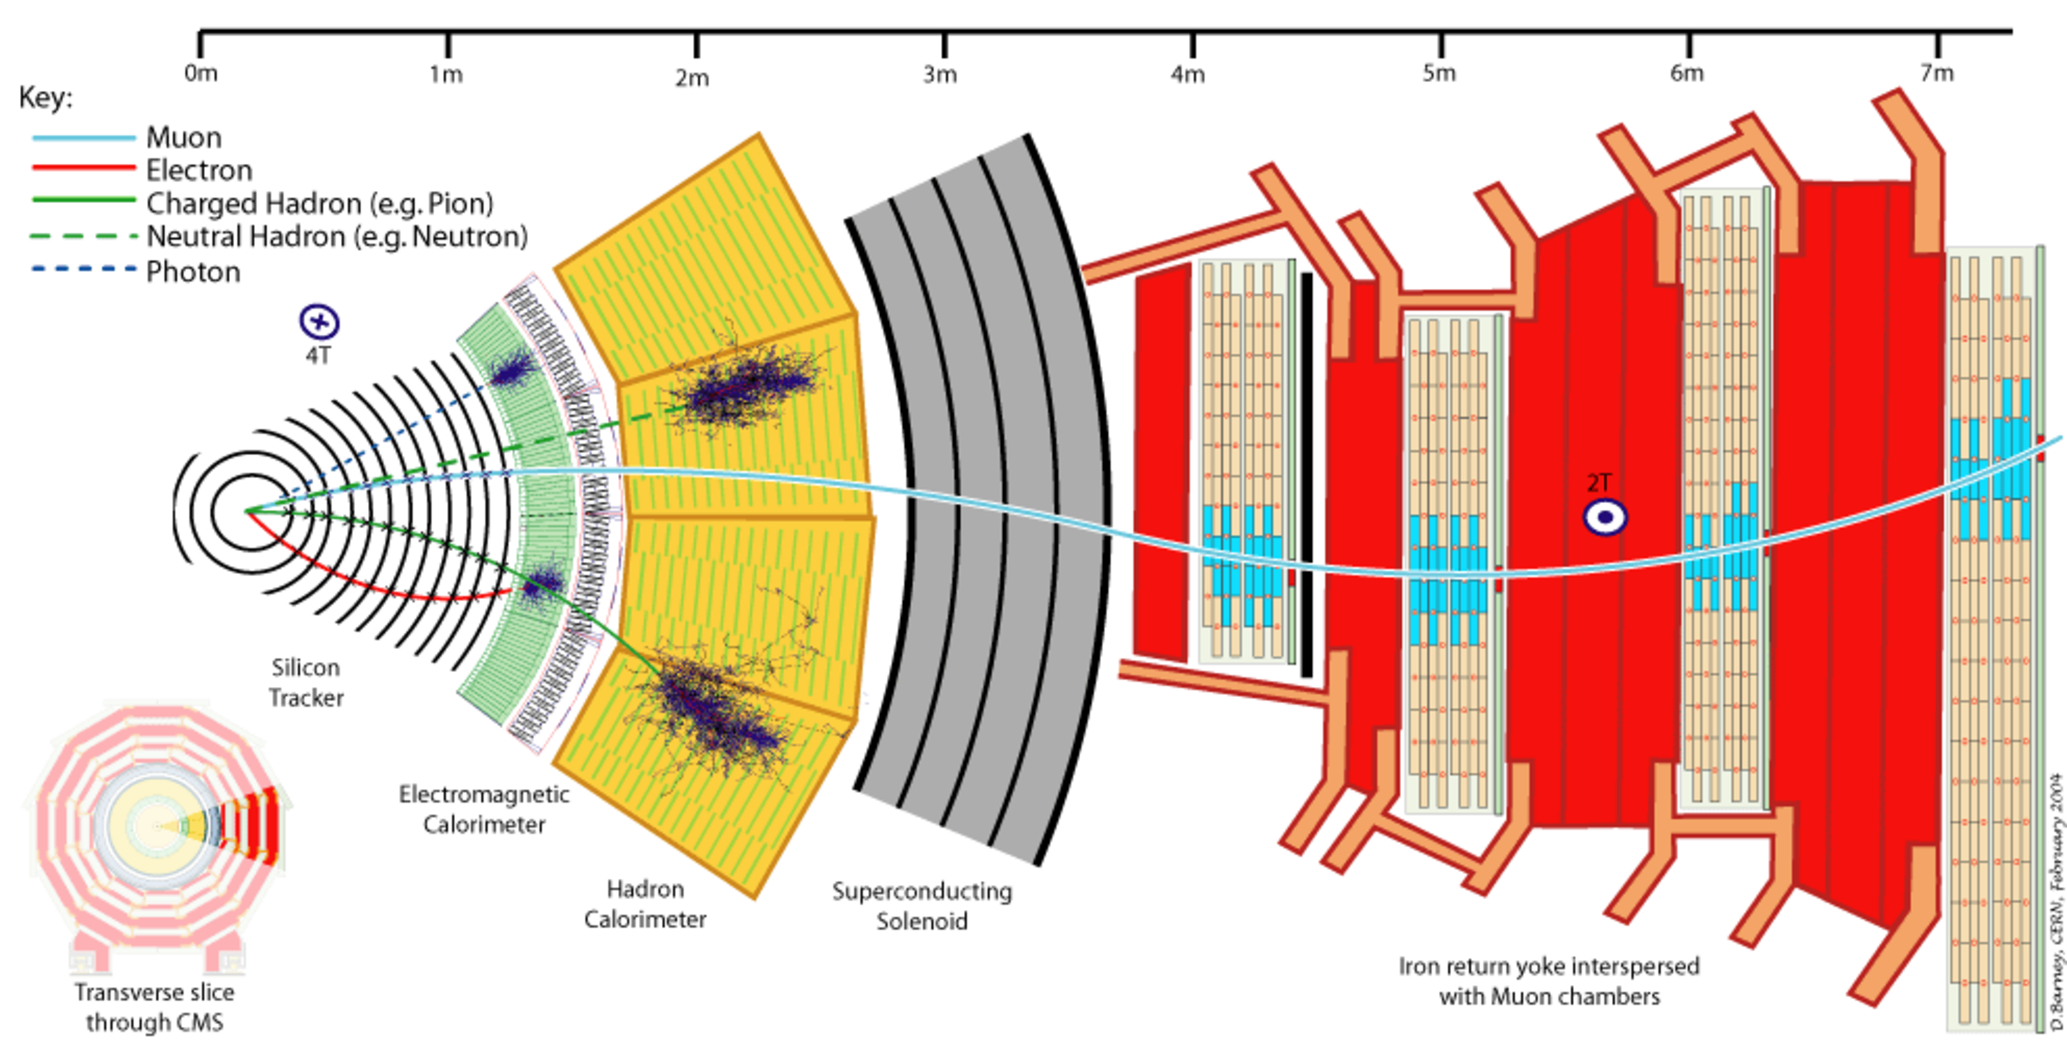
\includegraphics[width=0.8\textwidth]{ch4_figs/cms_particleflow.pdf}
   \caption{An overview of how CMS detects different types of particles. The slice of CMS in in the x-y plane.~\cite{cms_pflow_img}.}
   \label{fig:cms_pflow}
 \end{center}
\end{figure}

Object reconstruction begins with grouping collections of hits into tracks in an iterative process~\cite{CMS-TRK-09-001}. In the first iteration, tracks are
seeded with initial hits and subject to very tight criteria, sacrificing efficiency for a low fake rate. In the following iterations, hits assigned to
tracks in the previous iteration are removed from further consideration, and the criteria for candidate tracks is gradually relaxed with each iteration. In the final iterations,
the constraints on the track seed are relaxed to account for secondary decays from photon conversions and nuclear interactions with the silicon tracker material. This technique
reconstructs tracks with as few as three hits and \pts as small as 150 MeV with a fake rate in the single digits~\cite{CMS-PFT-09-001}. A similar but separate track
reconstruction is performed in the muon chambers to reconstruct muon tracks. 

Object reconstruction continues in the calorimeters, where it relies on a clustering algorithm to identify individual energy deposits and associate them to an object. This
algorithm is designed to yield a high efficiency even for low energy, and nearby objects. The clustering process is performed separately in the ECAL and HCAL, and furthermore in
the barrel, and endcaps. The ECAL preshower also uses separate clusterings in each of its two layers. In the HF, no clustering is performed, where each module is considered an
independent cluster. The clustering algorithm begins by identifying cells (cluster seeds) with an energy above a given ``seed'' energy threshold. Clusters are then increased by
adding adjacent\footnote{sharing at least one edge with the seed} cells that have an energy above a given threshold. The calorimeter granularity is used to optimize the
determination of cluster energies and positions~\cite{CMS-PFT-09-001}.  

After the tracking and clustering is complete, Particle Flow then matches tracks in the tracker to energy clusters in the calorimeters, and to tracks in the muon chambers.
In a given event, there can be many different objects and Particle Flow utilizes
a process-of-elimination strategy. Because they are the easiest to identify unambiguously, muons are identified first by matching tracks in the inner tracker to the tracks in
the muon chambers. The matching criteria is based on a $\chi^{2}$ fit threshold. When multiple sets of tracks are matched, the set with the lowest $\chi^{2}$ is selected as the
muon object. Muons are first reconstructed this way and called global muons. Particle flow muons are identifed from global muons when the \pt~s measured in the tracker and the
muon chambers agree to within three standard deviations. The tracks corresponding to the muon object are then removed from consideration for the remaining object reconstruction. 

Following muons, electrons are reconstructed next. Because electrons deflect strongly in the magnetic field, they leave characteristically short tracks, and lose energy via
Bremsstrahlung radiation. The tracks are flagged based on these characteristics as potential electron candidates and refitted with a Gaussian-Sum Filter (GSF)~\cite{gsf} and the
resulting tracks are then matched to ECAL energy clusters. The Bremsstrahlung photons are emitted tangentially to electron track and this is accounted for in the ECAL clustering
and track matching specifically for electrons. These matches are then subject to additional quality criteria before they are considered particle flow electrons, and their
corresponding tracks and energy deposits removed from further consideration for the remaining object reconstruction. 

At this point in the event/object reconstruction, the so-called low lying fruit has been picked, and the more difficult objects are all that remain. These objects are charged
and neutral hadrons (jets), and photons. The neutral particles are difficult to reconstruct because they don't leave hits in the tracker, so only calorimeter information is
available. Photons are distinguished from neutral hadrons by separate ECAL and HCAL clusters. Photons interact with and are stopped by the ECAL, while the same is true for
neutral hadrons and the HCAL. Additional in-event calibration techniques are also used to further distinguish these objects. The remainig tracks are subject to tighter
quality cuts aimed at reducing the fake-rate. The high-quality tracks passing these thresholds are matched to ECAL and HCAL deposits, and give rise to particle flow 
charge hadrons. The momentum of these objects is measured from the track radius and compared to the corresponding energy deposit in the calorimeters assuming the object is
a charged pion. If the two measurements are compatible, the momenta is refined with additonal fits to the tracks and energy deposit(s)~\cite{CMS-PFT-09-001}.

The charged and neutral hadron objects with tracks and matched energy deposits are only considered particle flow candidates at this stage.
An additional clustering step is necessary to reconstruct jet objects. As mentioned previously, when free quarks produced in the pp collision decay in the
fragmentation/hadronization process, they produce energetic and collimated sprays of charged
and neutral hadrons, called jets. To accurately determine the direction and momentum of the initial quark, as many of the corresponding charged and neutral hadrons as possible must not only be
reconstructed correctly and identified, but also clustered together (matched) correctly.
These jets are then intrepreted experimentally to be the free quark. An depiction of the hadronization and jet detection process is below in Figure~\ref{fig:frag}.

\begin{figure}[hbtp]
 \begin{center}
   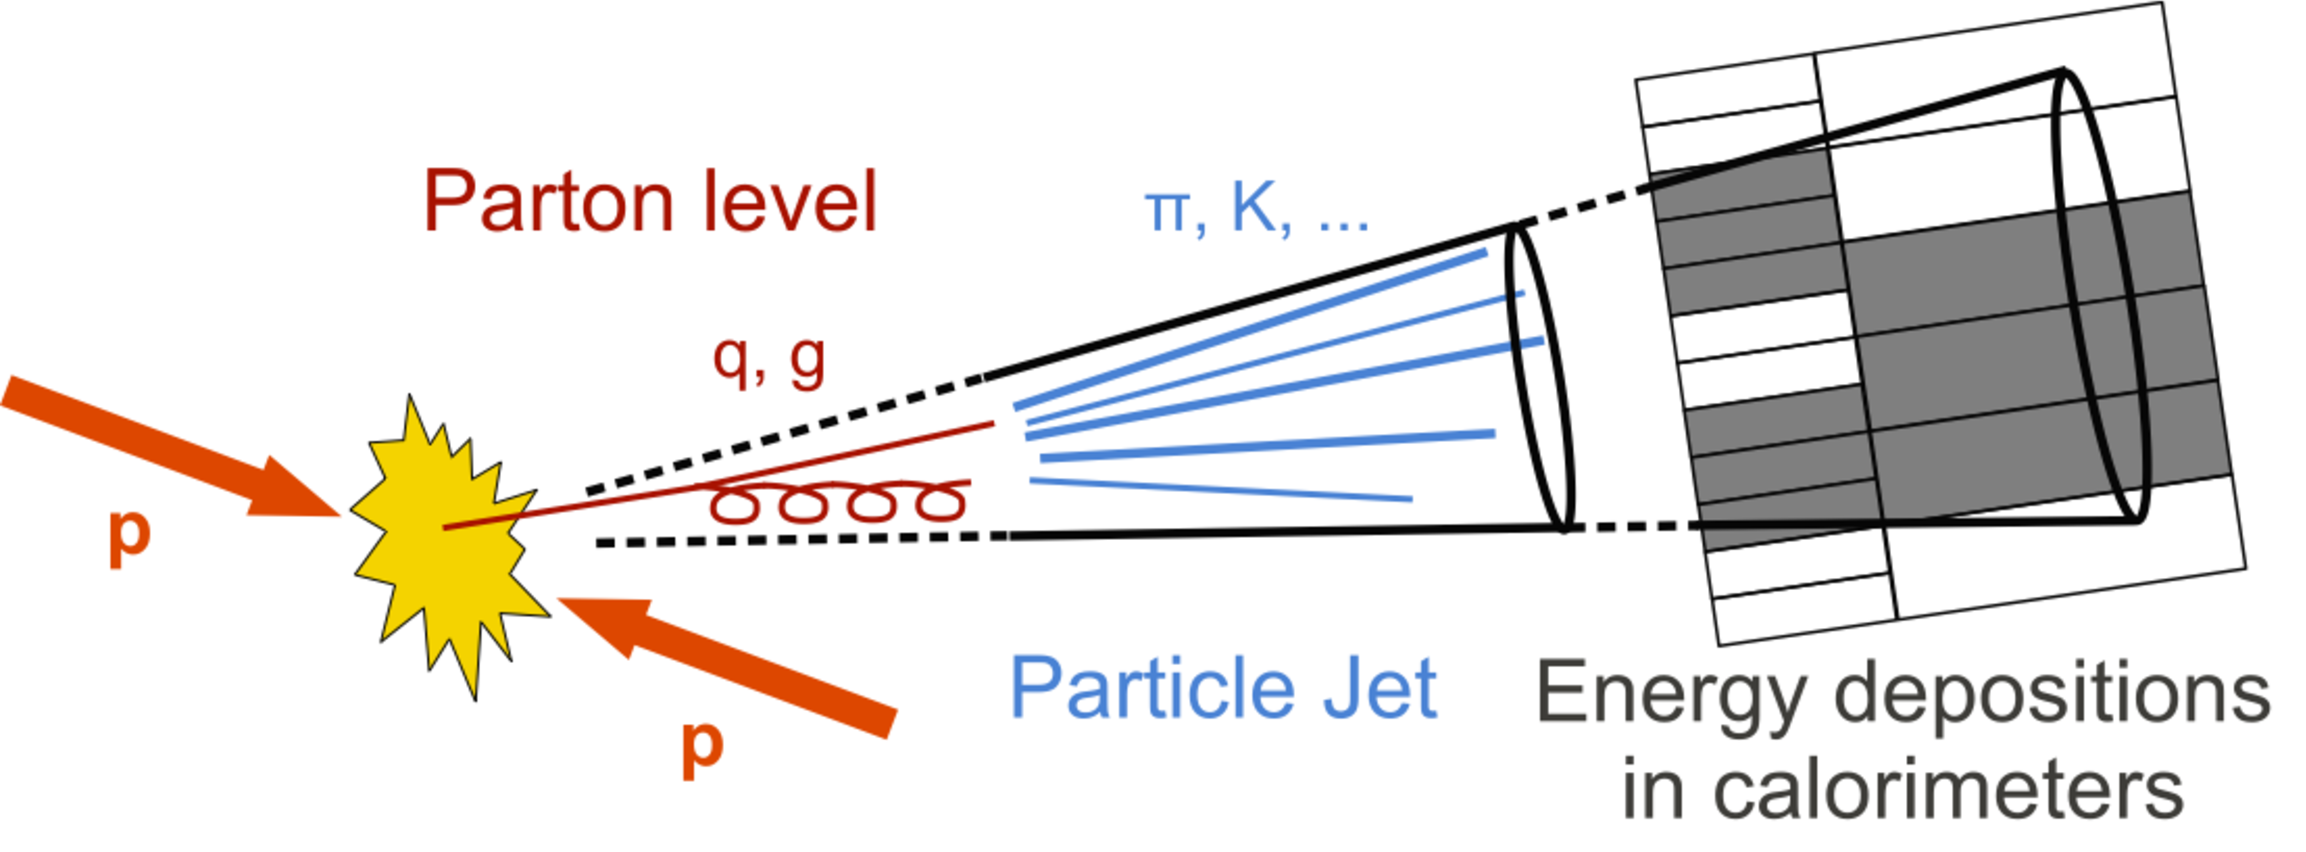
\includegraphics[width=0.8\textwidth]{ch4_figs/jet_frag.pdf}
   \caption{An example of quark hadronization and the resulting jet.~\cite{frag}.}
   \label{fig:frag}
 \end{center}
\end{figure}
 
Unfortunately, there are too many PF candidates detected and reconstructed in the calorimeters in a given event at one time to make the jet clustering process straight-forward
and unambiguous. To address this, jet clustering algorithms are used for clustering. These algorithms exploit information from the detector with theoretical knowledge of the
hadronization process to cluster the jets sensible and reproducible manner.
While many clustering algorithms exist, the one used by this analysis is the anti-$k_{T}$ algorithm~\cite{antikt}. Anti-$k_{T}$ begins like other sequential clustering algorithms,
by calculating the distance measures in equations~\ref{eqn:antikt1}. 

\begin{equation}
\begin{aligned}
\label{eqn:antikt1}
%%\begin{split}
d_{ij} &= min(k^{2p}_{Ti},k^{2p}_{Tj})\frac{\Delta_{ij}^{2}}{R^{2}} \\ d_{iB} &= k^{2p}_{Ti}
%%\end{split}  
\end{aligned} 
\end{equation}

\noindent where $\Delta_{ij}^{2} = (y_{i}-y_{j})^{2} + (\phi_{i}-\phi_{j})^{2}$ and $y_{i}$,$k_{Ti}$ are the rapidity and momenta of particle i respectively. After the
distance measures have been calculated for each candidate in the event, the smallest $d_{ij}$ are merged into one object by summing the 4-momenta of particles i and j, the
distance measures are updated and the algorithm moves onto the next smallest $d_{ij}$. If a particle has the smallest $d_{iB}$, it is removed and called a jet. This
iterative process continues until all PF candidates are clustered into jets. What differentiates anti-$k_{T}$ from Cambridge-Aachen and other similar algoirthms is the choice
of p = -1 in equation~\ref{eqn:antikt1}. This negative value explains the name of the algorithm, and the tendancy for it to produce circular\footnote{circular in the
$\eta$-$\phi$ plane} jets, centered on the highest \pt~candidate of the jet. The effect of these parameter values with respect to other available algorithms is below in
Figure~\ref{fig:jet_cluster}.

\begin{figure}[htbp] 
  {\centering
    \subfigure[$k_{T}$]{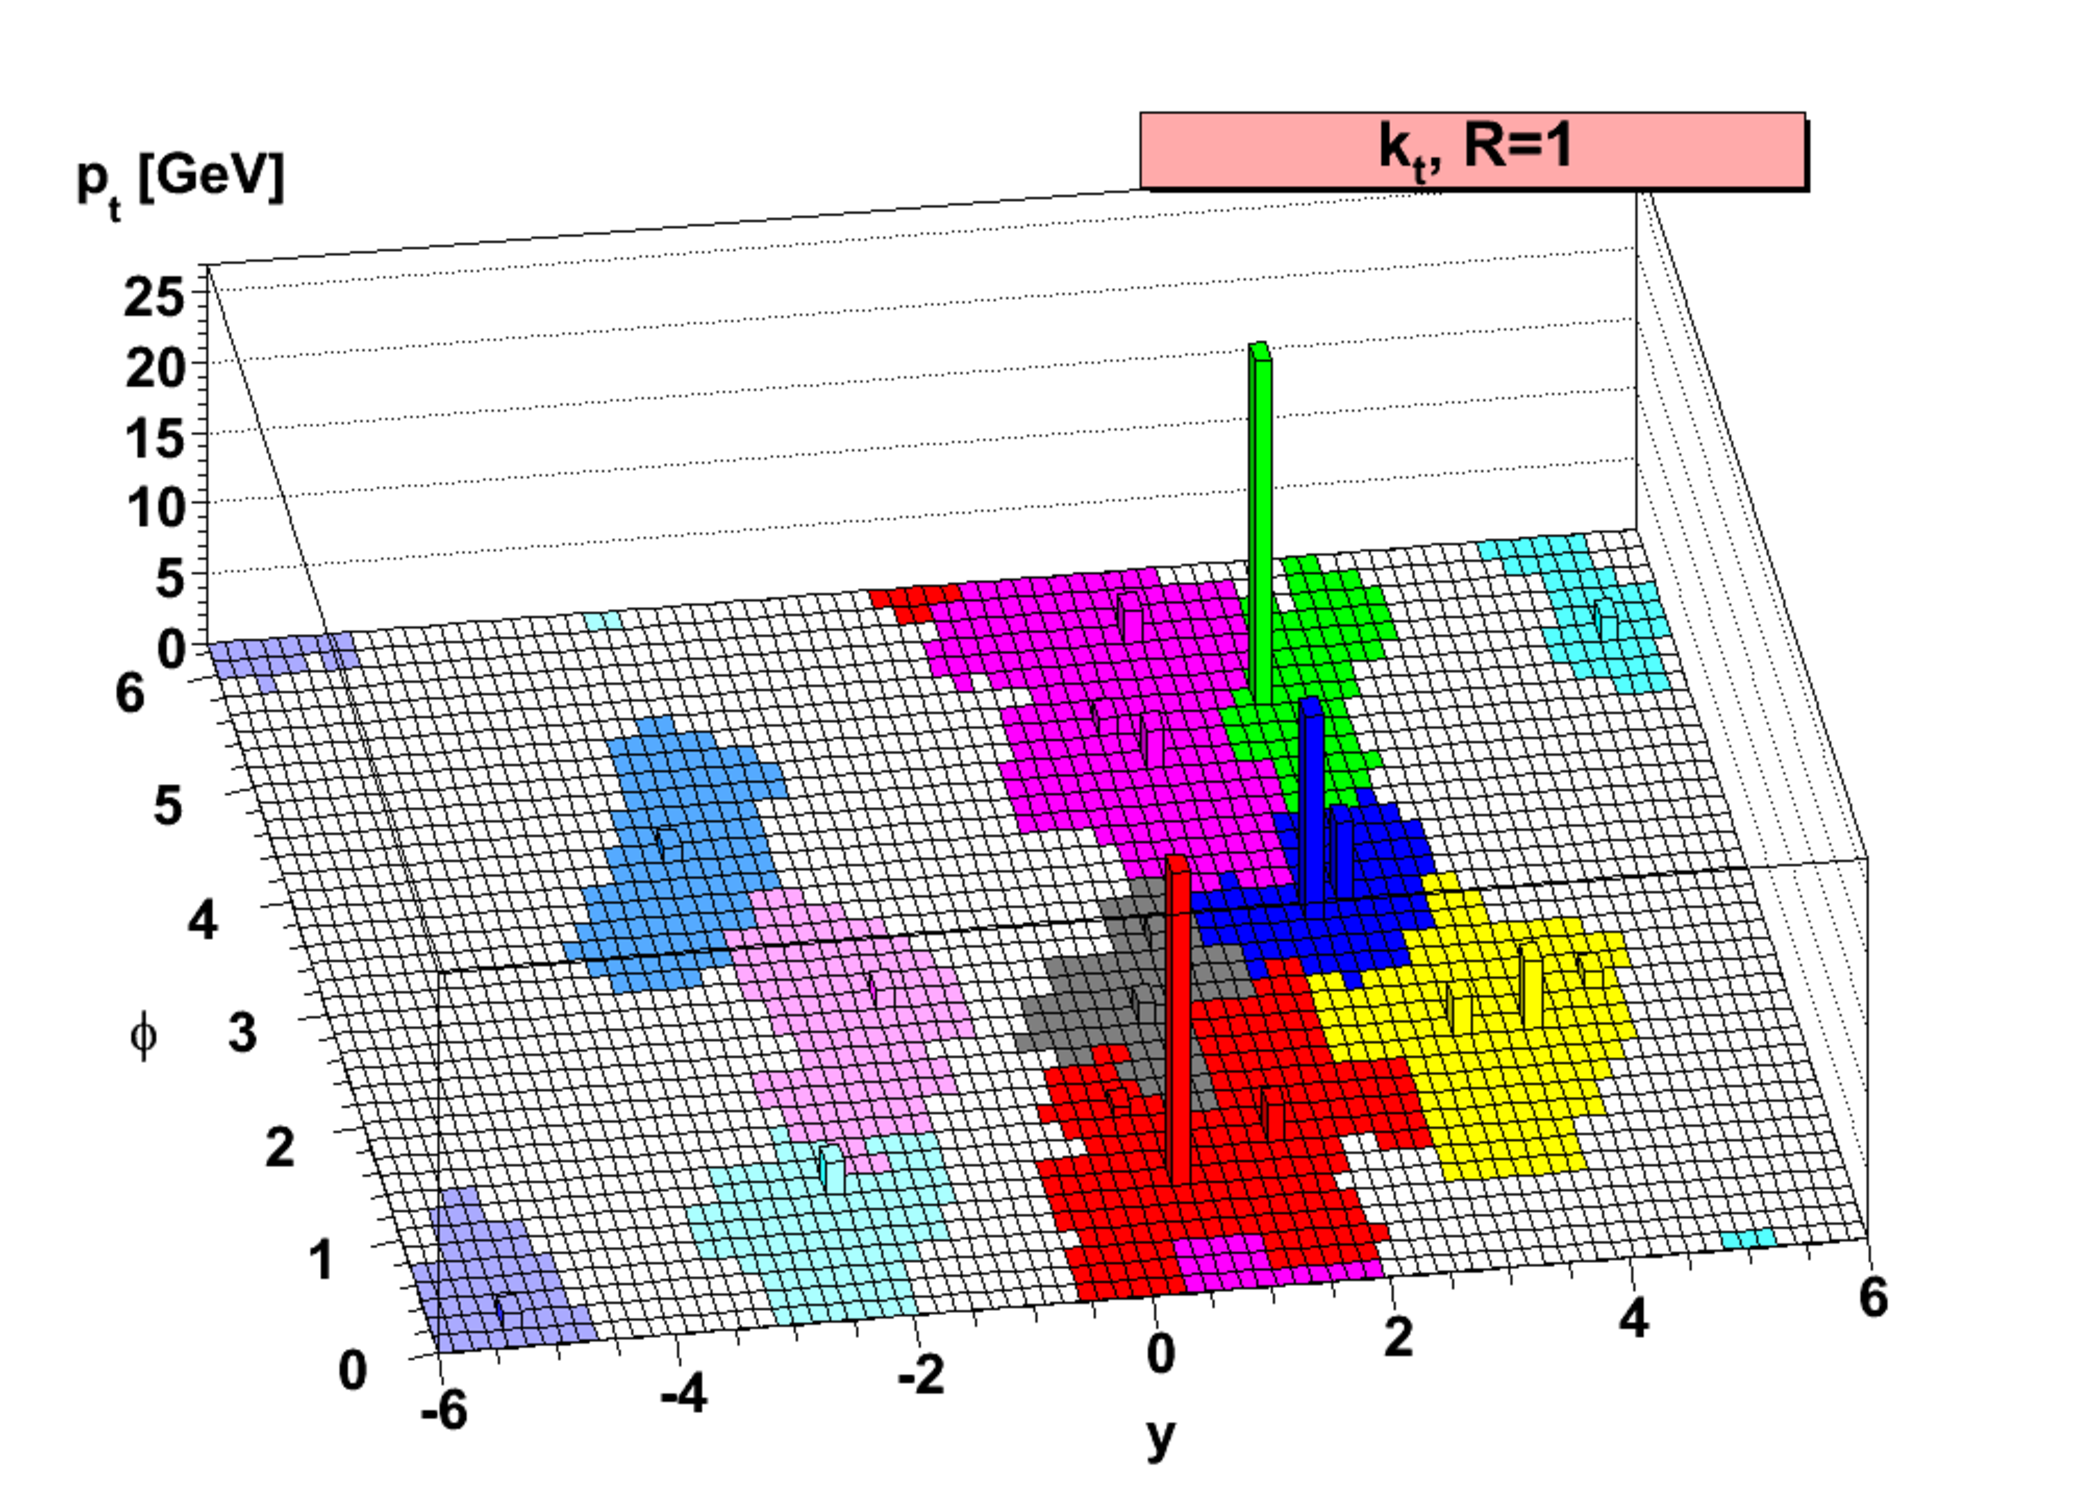
\includegraphics[width=0.4\textwidth]{ch4_figs/kt.pdf}}
    \subfigure[Cambridge-Aachen]{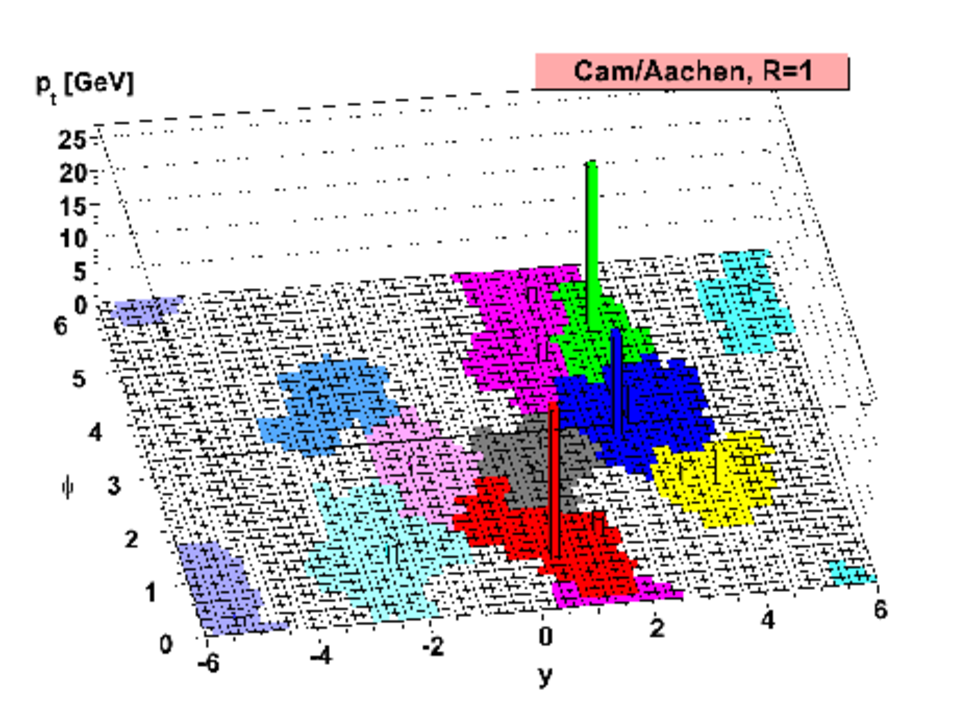
\includegraphics[width=0.4\textwidth]{ch4_figs/ca.pdf}}
    \subfigure[SIScone]{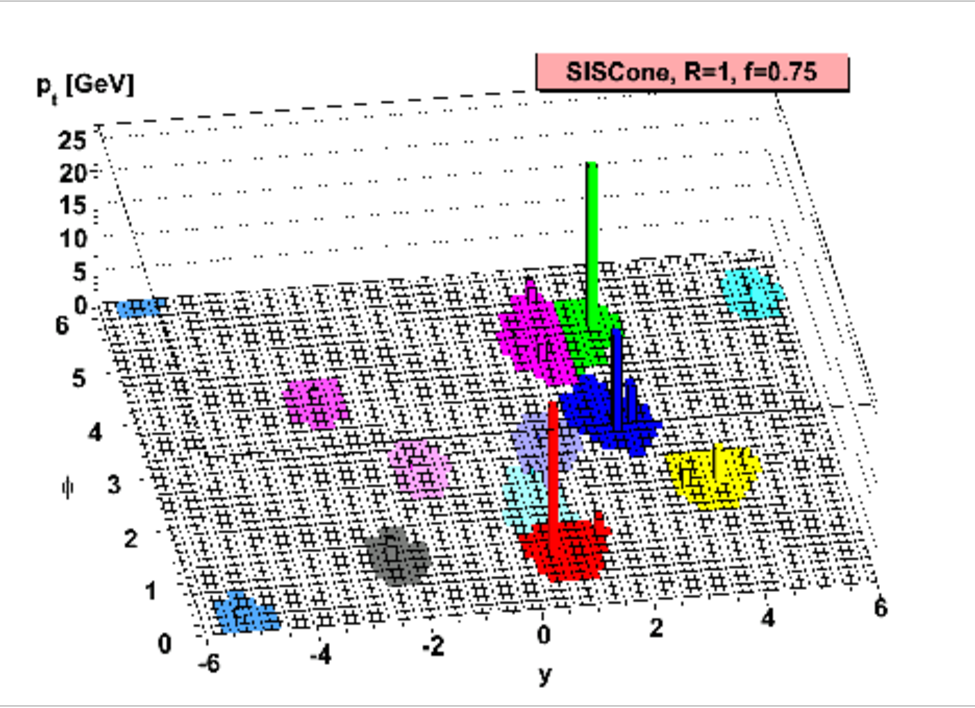
\includegraphics[width=0.4\textwidth]{ch4_figs/sis.pdf}}
    \subfigure[anti-$k_{T}$]{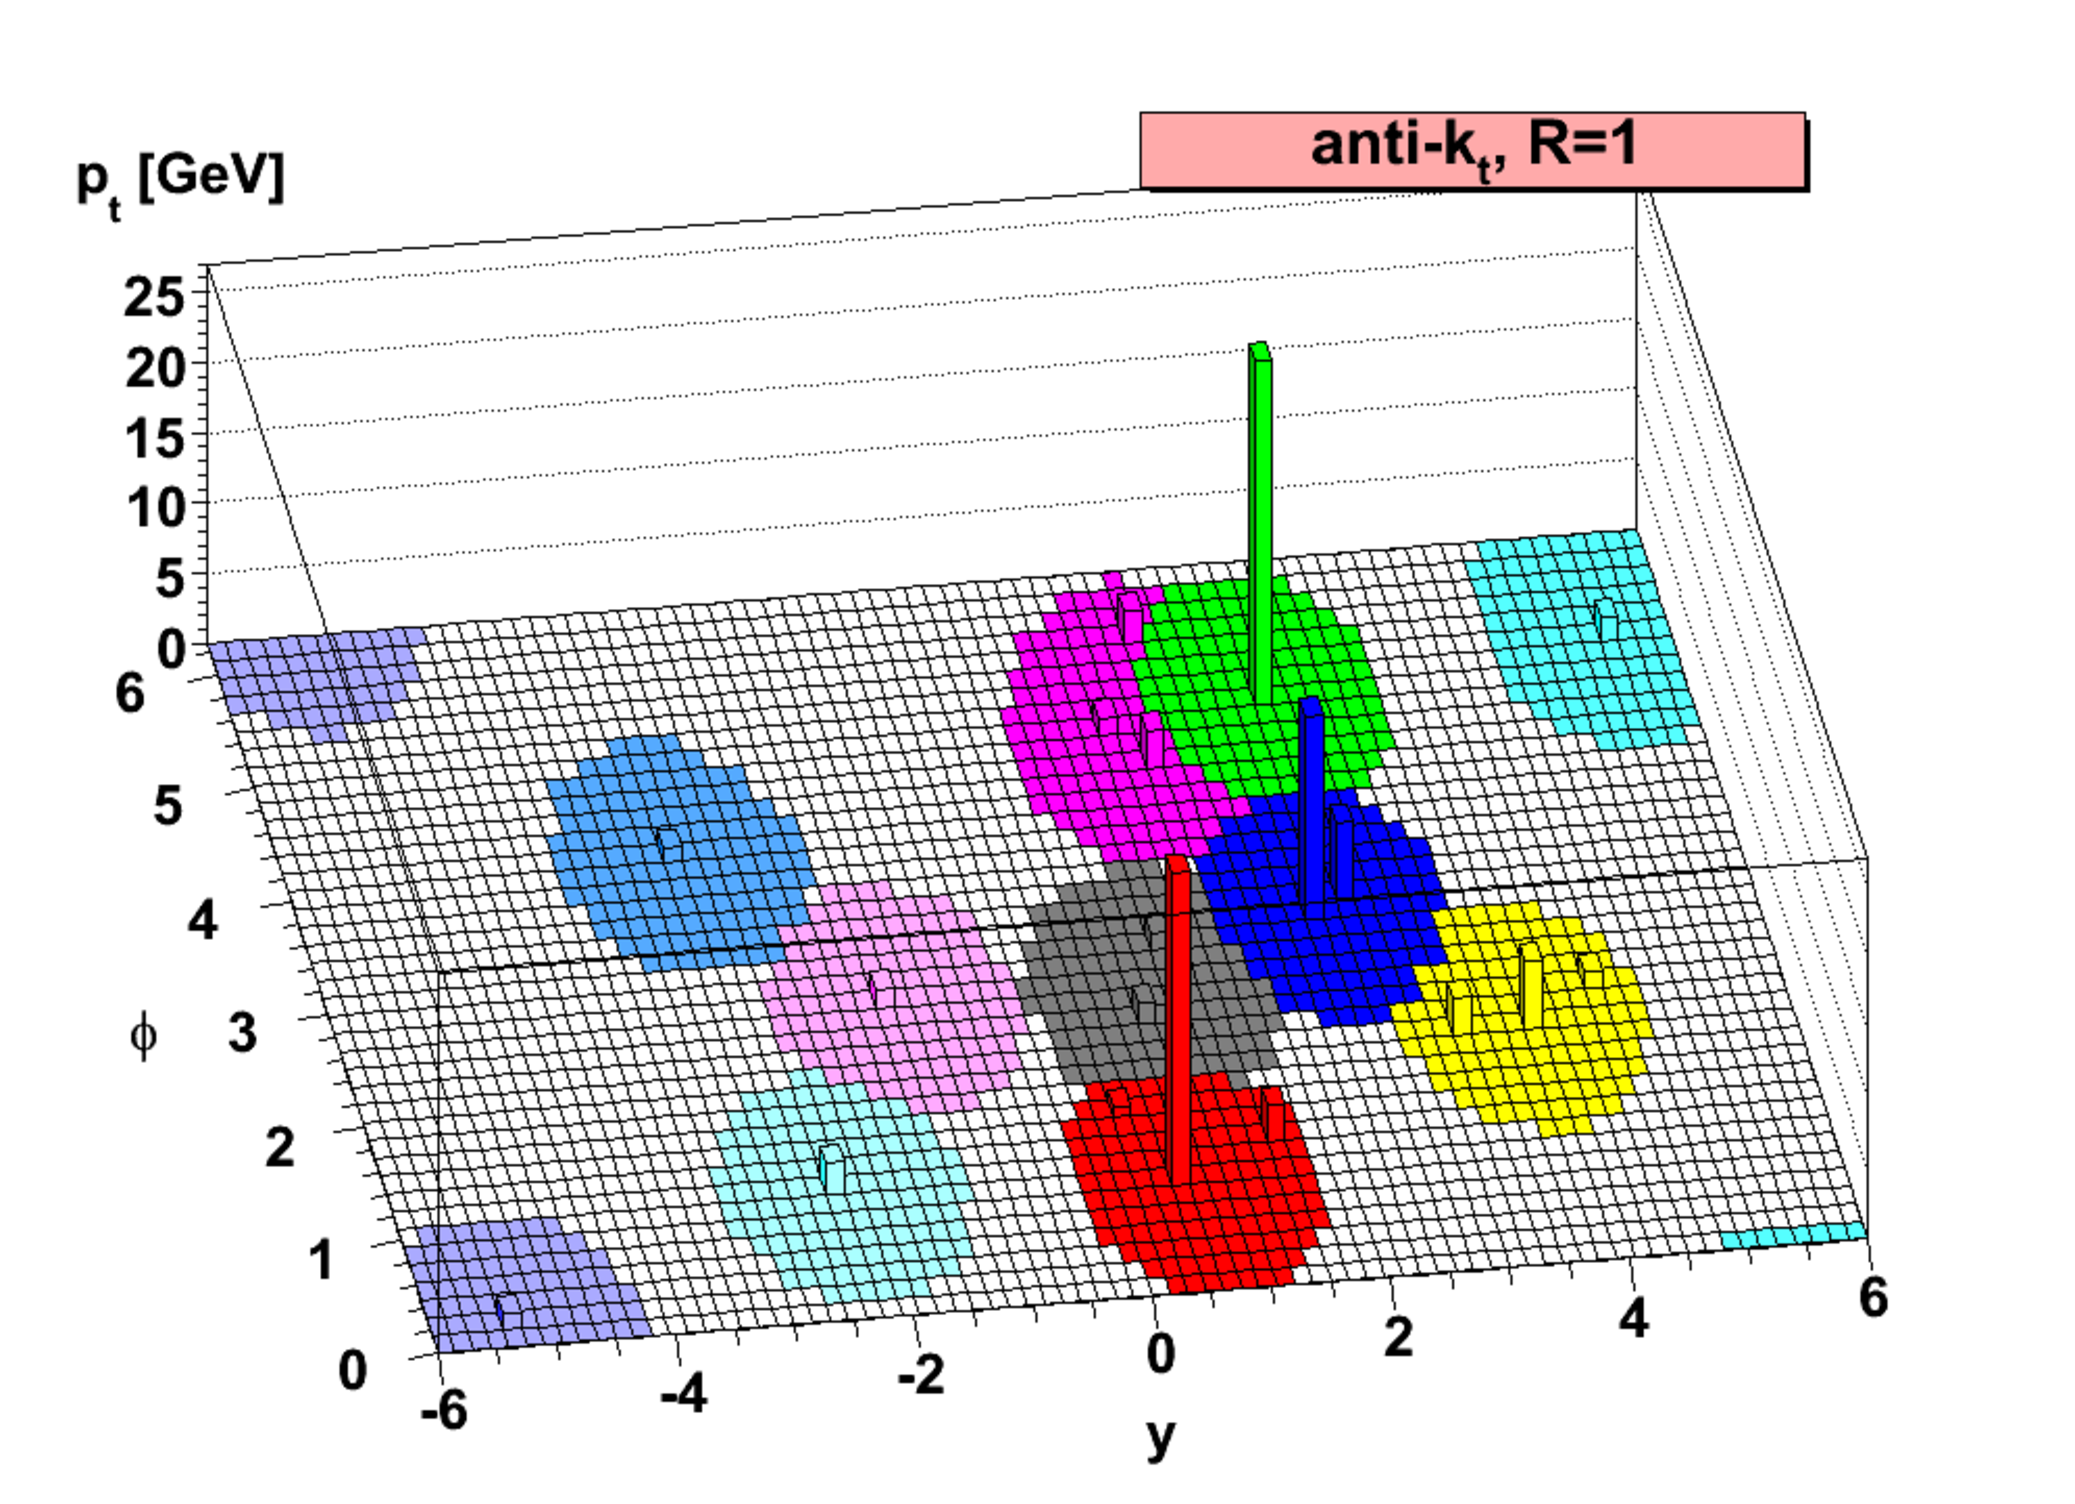
\includegraphics[width=0.4\textwidth]{ch4_figs/akt.pdf}}
    \caption{Jets in a sample MC event clustered with various algorithms.
    \label{fig:jet_cluster}}
\end{figure}

The final parameter in equation~\ref{eqn:antikt1} is defined as $R = \sqrt{\Delta\eta^{2}+\Delta\phi^{2}}$ is the conesize of the jet being clustered.
The cone size used for clustering in this analysis is R = 0.4. Versions of this analysis on 7, and 8 TeV datasets used a wider cone of 0.5. The move to smaller cone size
was motivated by the fact that jets tend to be more energetic and thus narrower and more collimated as the center-of-mass collision energy increases to 13 TeV. All techniques
mentioned above proved CMS analyzers the basic physics objects needed to perform analysis, and also standardizes the object reconstruction across the experiment. 

\section{Primary Vertex Identification and Pile-up}
Due to the way the LHC collides bunches, there are multiple pp collisions in each LHC bunch crossing at CMS. Unfortunately, many of these collisions produce
multiple objects that are reconstructed, but only 1 of these collisions is considered a hard scatter head-on collision capable of producing a \tth event.
These additional collisions that don't include the hard scatter event of interest, as well as their resulting reconstructed objects are referred to as pile-up, because
they are said to pile up on top of the objects from the collision of interest.
The collision of interest is called the primary vertex.
In this analysis and also in many others, the primary vertex is defined as the vertex with the highest \pt~sum of all constituent tracks.  
Pileup is problematic because it can make matching objects to collisions difficult. Fortunately,
CMS has an excellent tracker which makes the process of matching tracks to vertices (collision) fairly straightforward. Aside from the tracking, pileup is also
problematic because the energy deposits in the calorimeters from the pilup objects can distort the energy measurements and clustering of objects originating from
the primary vertex. There are numerous techniques to account for these effects. The technique employed in this analysis is to assign an average amount of energy
due to pileup in the detector, and subtract it off from each reconstructed jet energy measurement. This is called the rho correction.  
An example of the reconstructed tracks and vertices in an
LHC bunch crossing is below in Figure~\ref{fig:pileup_vertices}.

\begin{figure}[hbtp]
 \begin{center}
   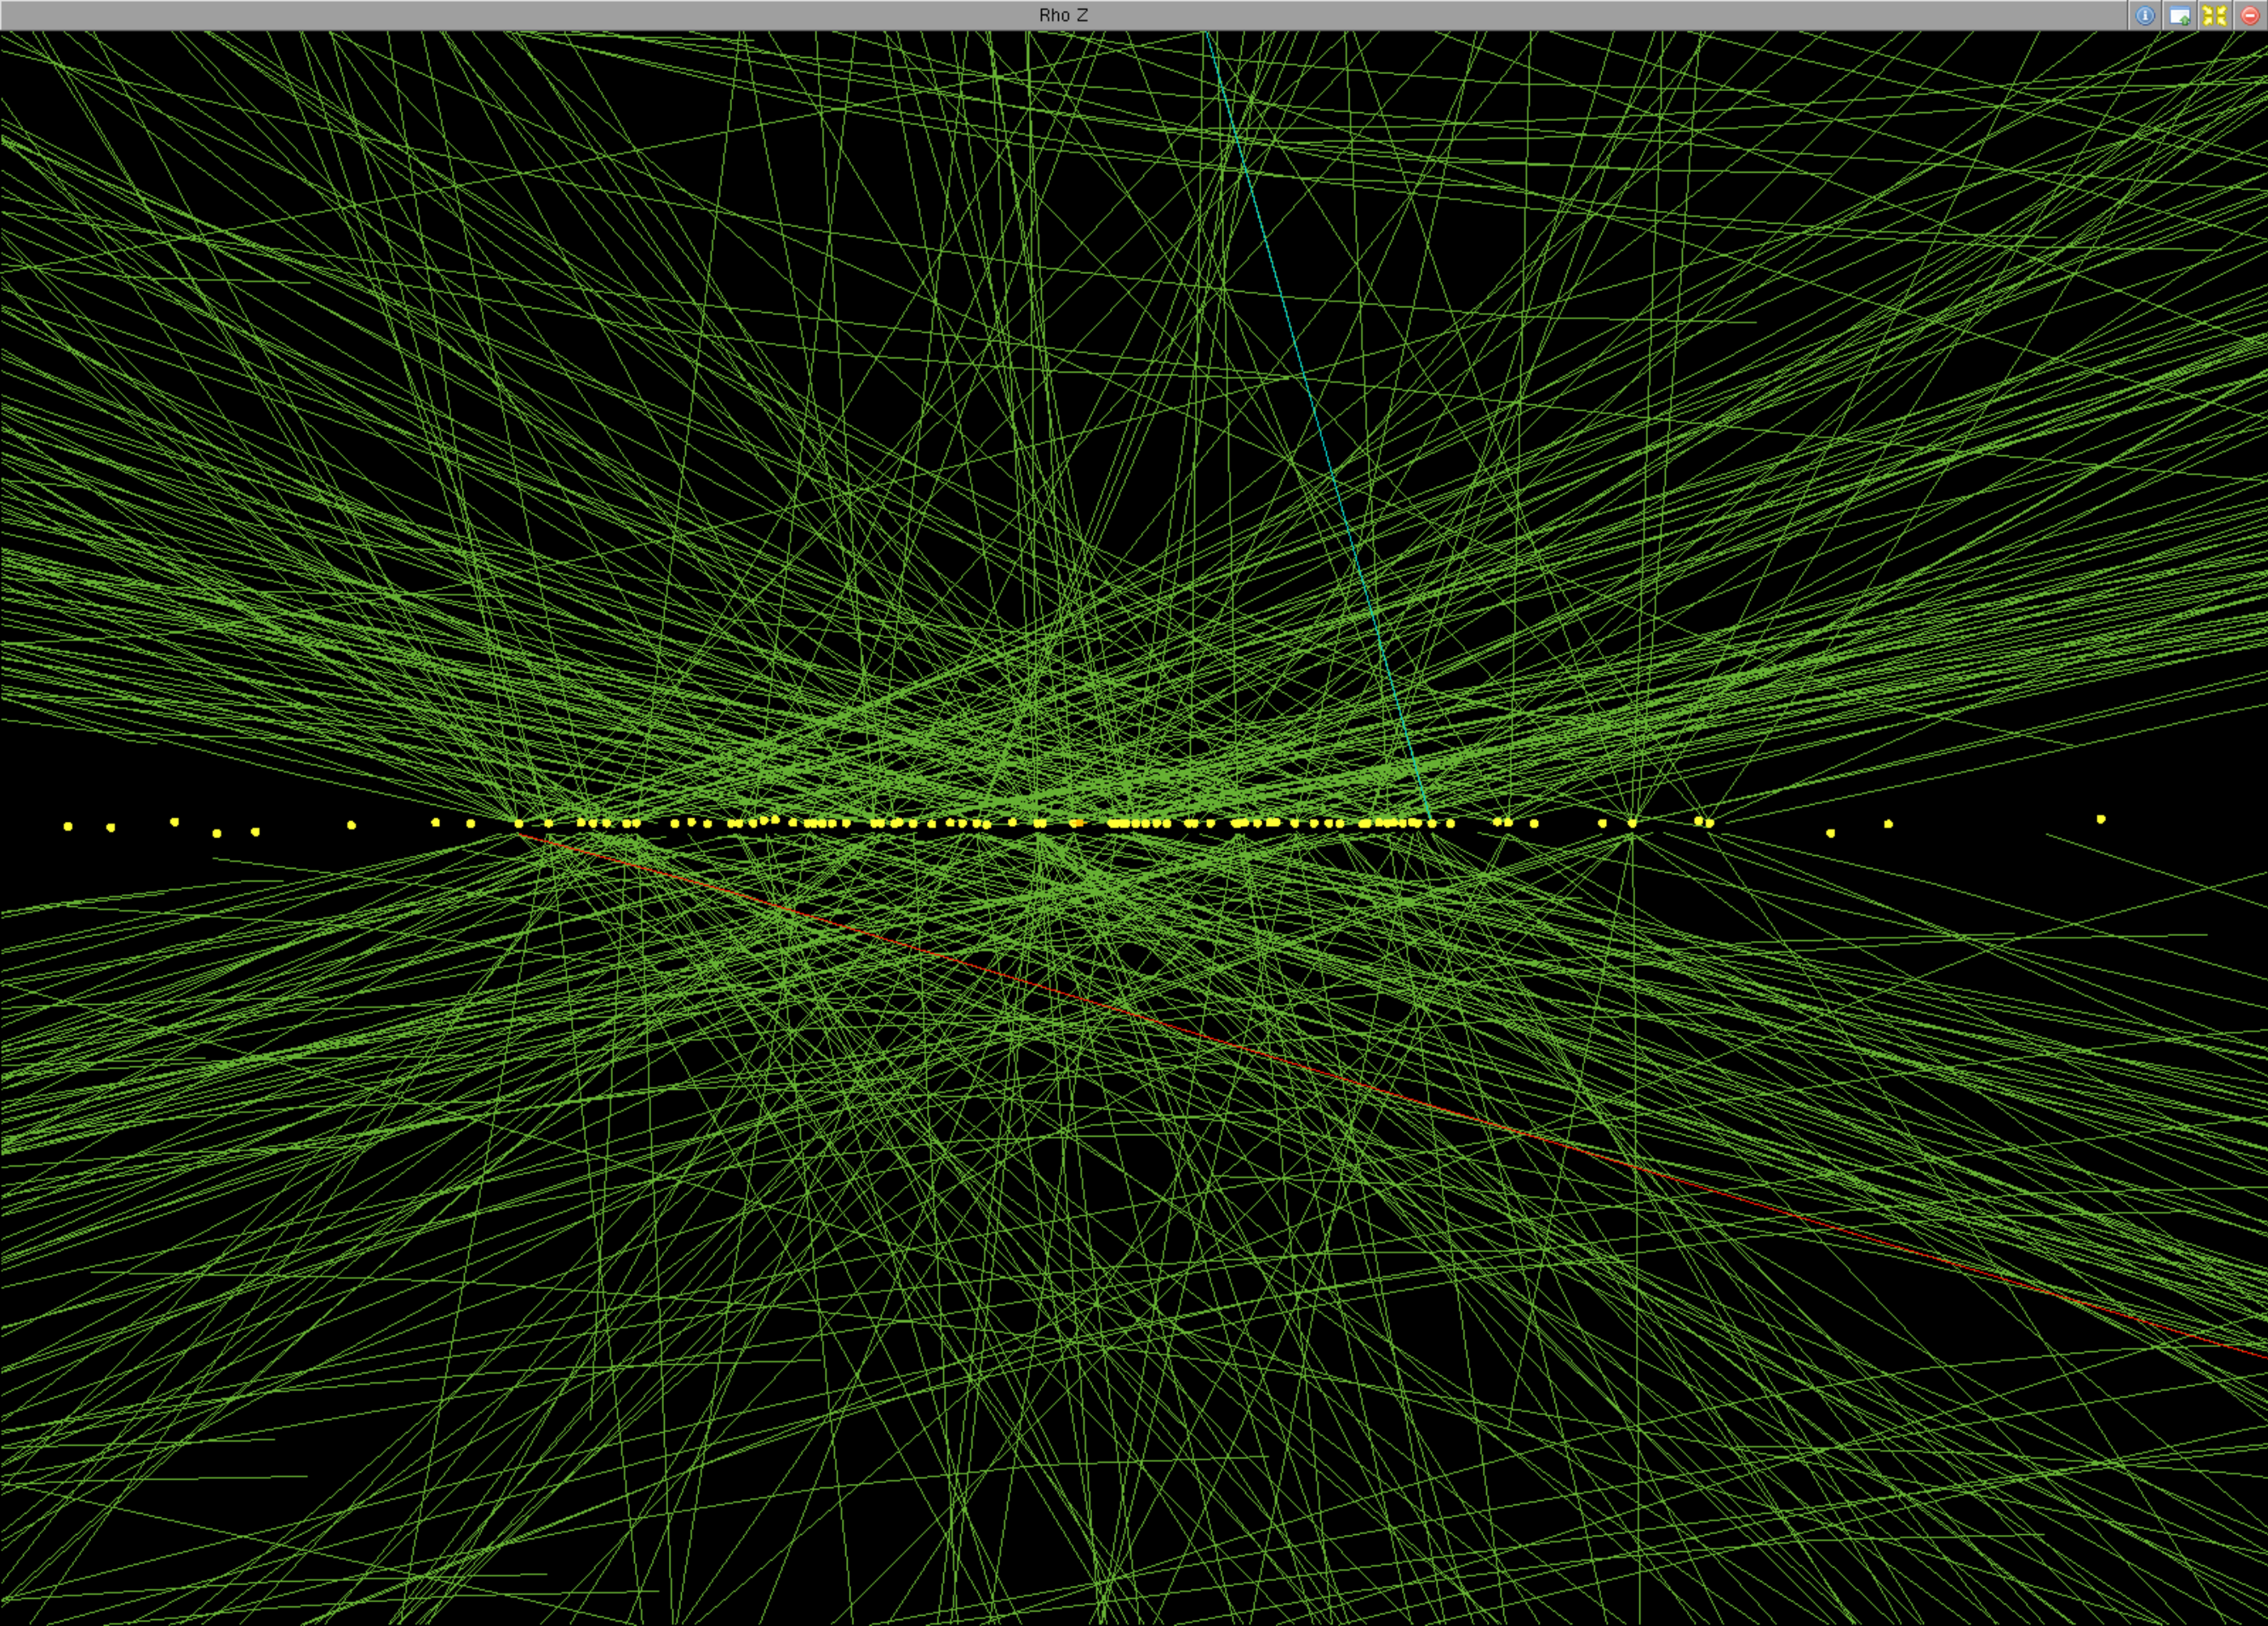
\includegraphics[width=0.8\textwidth]{ch4_figs/cms_pileup.pdf}
   \caption{A side view of the CMS tracker's reconstructed vertices in a special high pileup LHC run. The pileup in this here is 78, meaning there are
78 collisons in a single bunch crossing~\cite{pileup_image}.}
   \label{fig:pileup_vertices}
 \end{center}
\end{figure}

\noindent The pileup values in the data in this analysis varies from 30 to 45, meaning there are, on average, between 30 and 45 collisions (including the primary vertex) in each
bunch crossing recorded by CMS. 


\section{Object Selection}
After the basic object reconstruction is performed, each event is ready for the fist steps of analysis. The analysis begins with object selection where the objects in each
event are subjected to tighter criteria to ensure quality objects in the analysis that are consistent with signal and background predictions. This selection depends on and 
varies with the type of object desired in the event. Because the \tth multilepton final state is so complicated, almost\footnote{all objects except the photon, which are
used in the \tth,$H\rightarrow\gamma\gamma$ search} all objects available from the particle flow
reconstruction are needed to identify events that are consistent with the signal, namely jets, missing energy, charged leptons, and hadronic taus.

\subsection{Jets}
Jets are reconstructed from PF clusters 
\subsubsection{b-jet Identification}
\subsection{Missing Energy}
\subsection{Leptons}
\subsection{Taus}


%
% Chapter 5
%

\chapter{EVENT SELECTION}
\label{chap:event_selection}
The event selection defines the signal regions of this analysis. The signal regions are categories of events defined by requirements aimed at 
selecting as much signal (\tth), and simultaneously rejecting as much background as possible.
In the multilepton analysis, there are three signal regions predominantly defined by the lepton multiplicity in the event: the two-lepton same-sign ($2lss$) region,
the three-lepton ($3l$) region, and the four-lepton ($4l$) region. This dissertation focuses $2lss$ category. Defining the signal regions by lepton multiplicity is motivated
by the fact that the number of leptons passing the object selection yields the most information about the event.

There are several cuts which don't depend on lepton multiplicity that are applied to all signal regions to ensure the selection of events consistent with \tth. Events with
a pair of loose leptons with an invariant mass of less than 12 GeV are vetoed, as they are consistent with a J/$\psi$ or $\Upsilon$ decay and are not modeled in the MC
simulation, but are present in data. At least two jets are required in all signal regions, and of these there must be at least one jet passing the medium CSVv2 working point,
or two passing the loose working point. This b-jet requirement is consistent with a top-quark pair decaying to jets, which is present in all \tth processes. 

\section{Two-lepton same-sign category}
The $2lss$ category is primarily defined by the requirement that there be exactly two tight leptons that have the same sign electric charge. The same-sign requirement is needed to veto 
one of the largest backgrounds dileptonic \ttbar + jets, which has oppositely charged leptons and a cross section more than three orders of magnitude greater than that of \tth. We require
the leading lepton have \pt $>$ 25 GeV to stay well above the trigger threshold for reasons that will be explained in the trigger section. At least 4 jets are required, to be consistent with
a \tth process with two same-sign leptons in the final state. To reject backgrounds with Z bosons where one of the lepton charges is mis-measured, we reject any di-electron pair whose invariant
mass is within 10 GeV of the Z mass (90.2 GeV) and also require the \met LD be greater than 0.2 (again, for di-electron events only). To summarize, the $2lss$ category is defined by events
satisfying the collowing requirements:

\begin{itemize}
 \item Exactly two tight leptons with the same-sign electric charge and \pt $>$ 25,15 GeV
 \item m($ll$) $<$ 12 GeV for any pair of loose leptons in the event
 \item $\geq$4 jets, among which there must be $\geq$1 CSVv2 M or $\geq$2 CSVv2 L
 \item $|m(ee)-m_{Z}| >$ 10 GeV (for ee events only)
 \item \met LD $>$ 0.2 (for ee events only) 
\end{itemize}

\begin{figure}[htp]
\centering
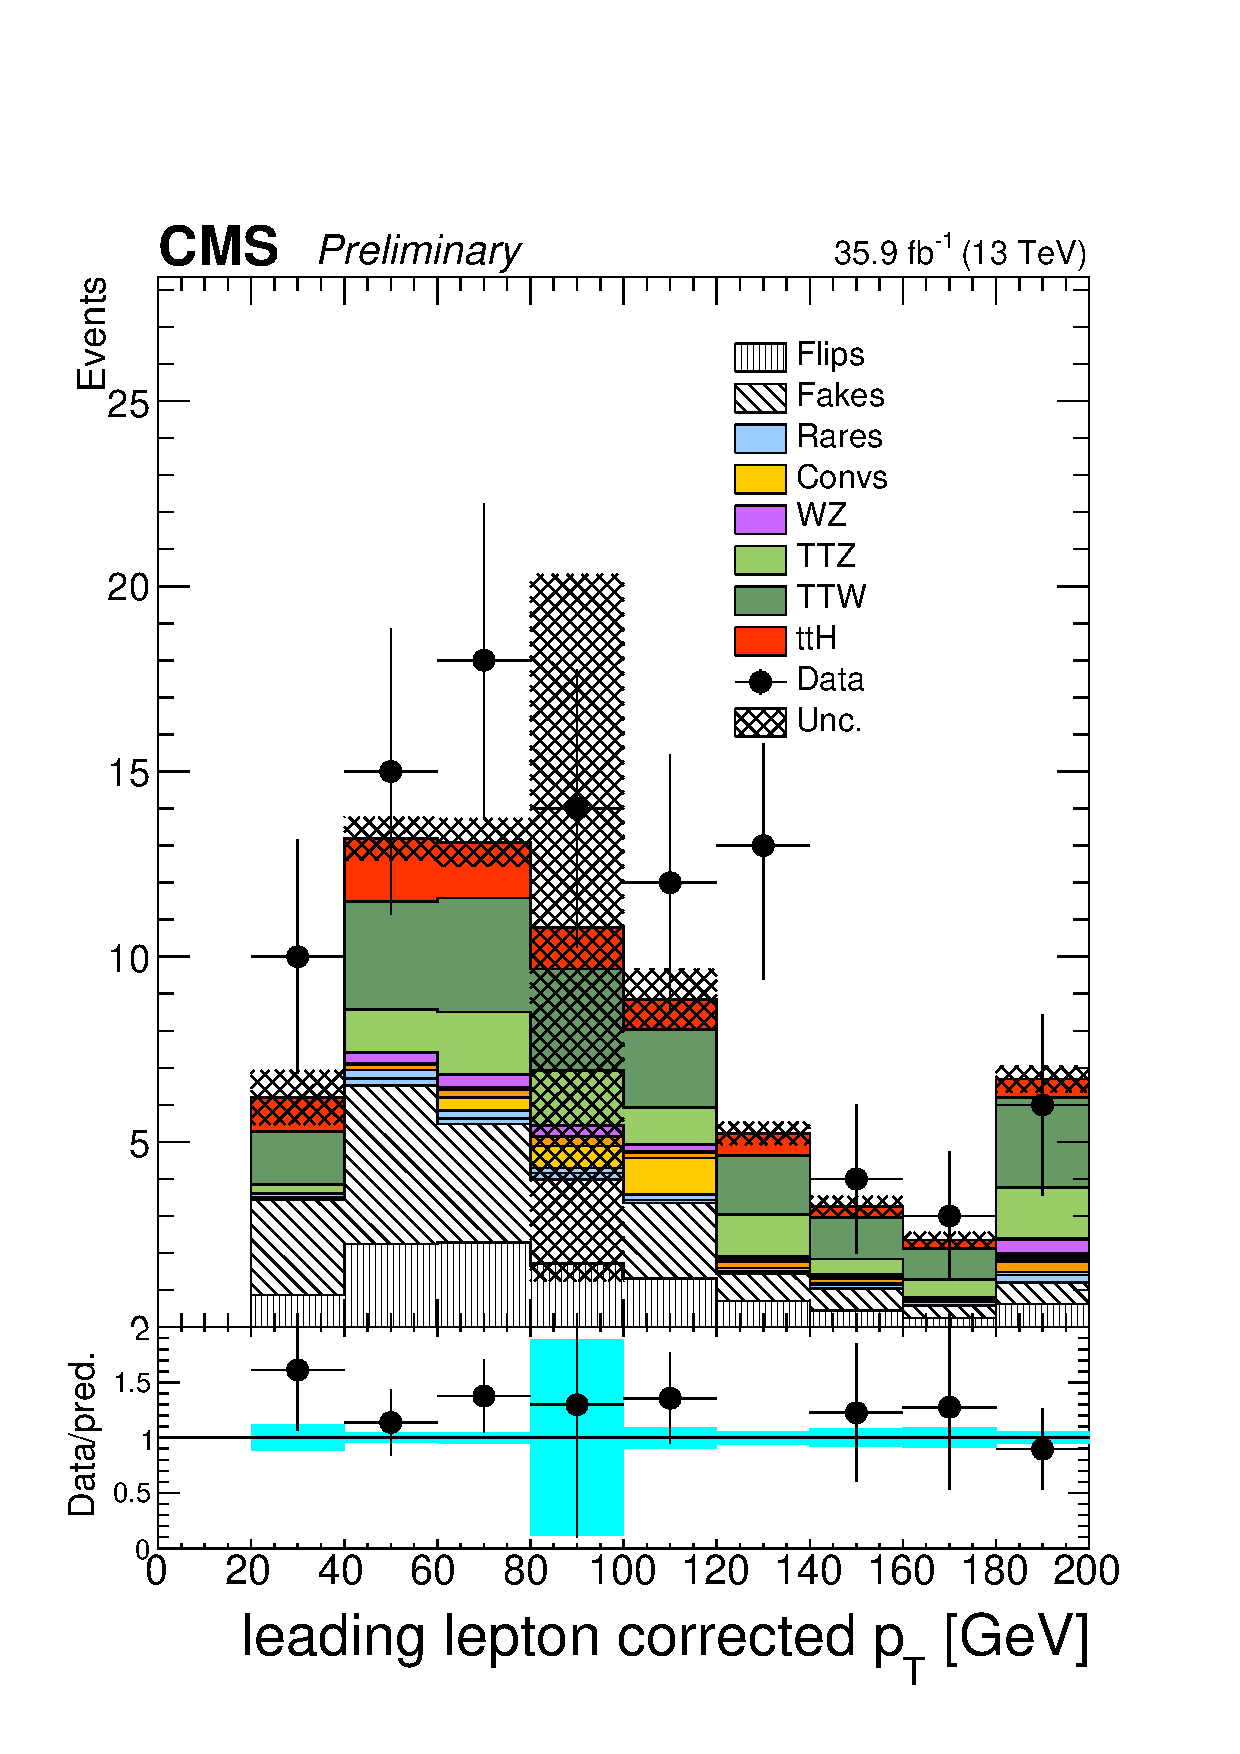
\includegraphics[width=0.32\textwidth]{ch5_figs/l1_pt_ttH_ee_stackPlot_SR.pdf}
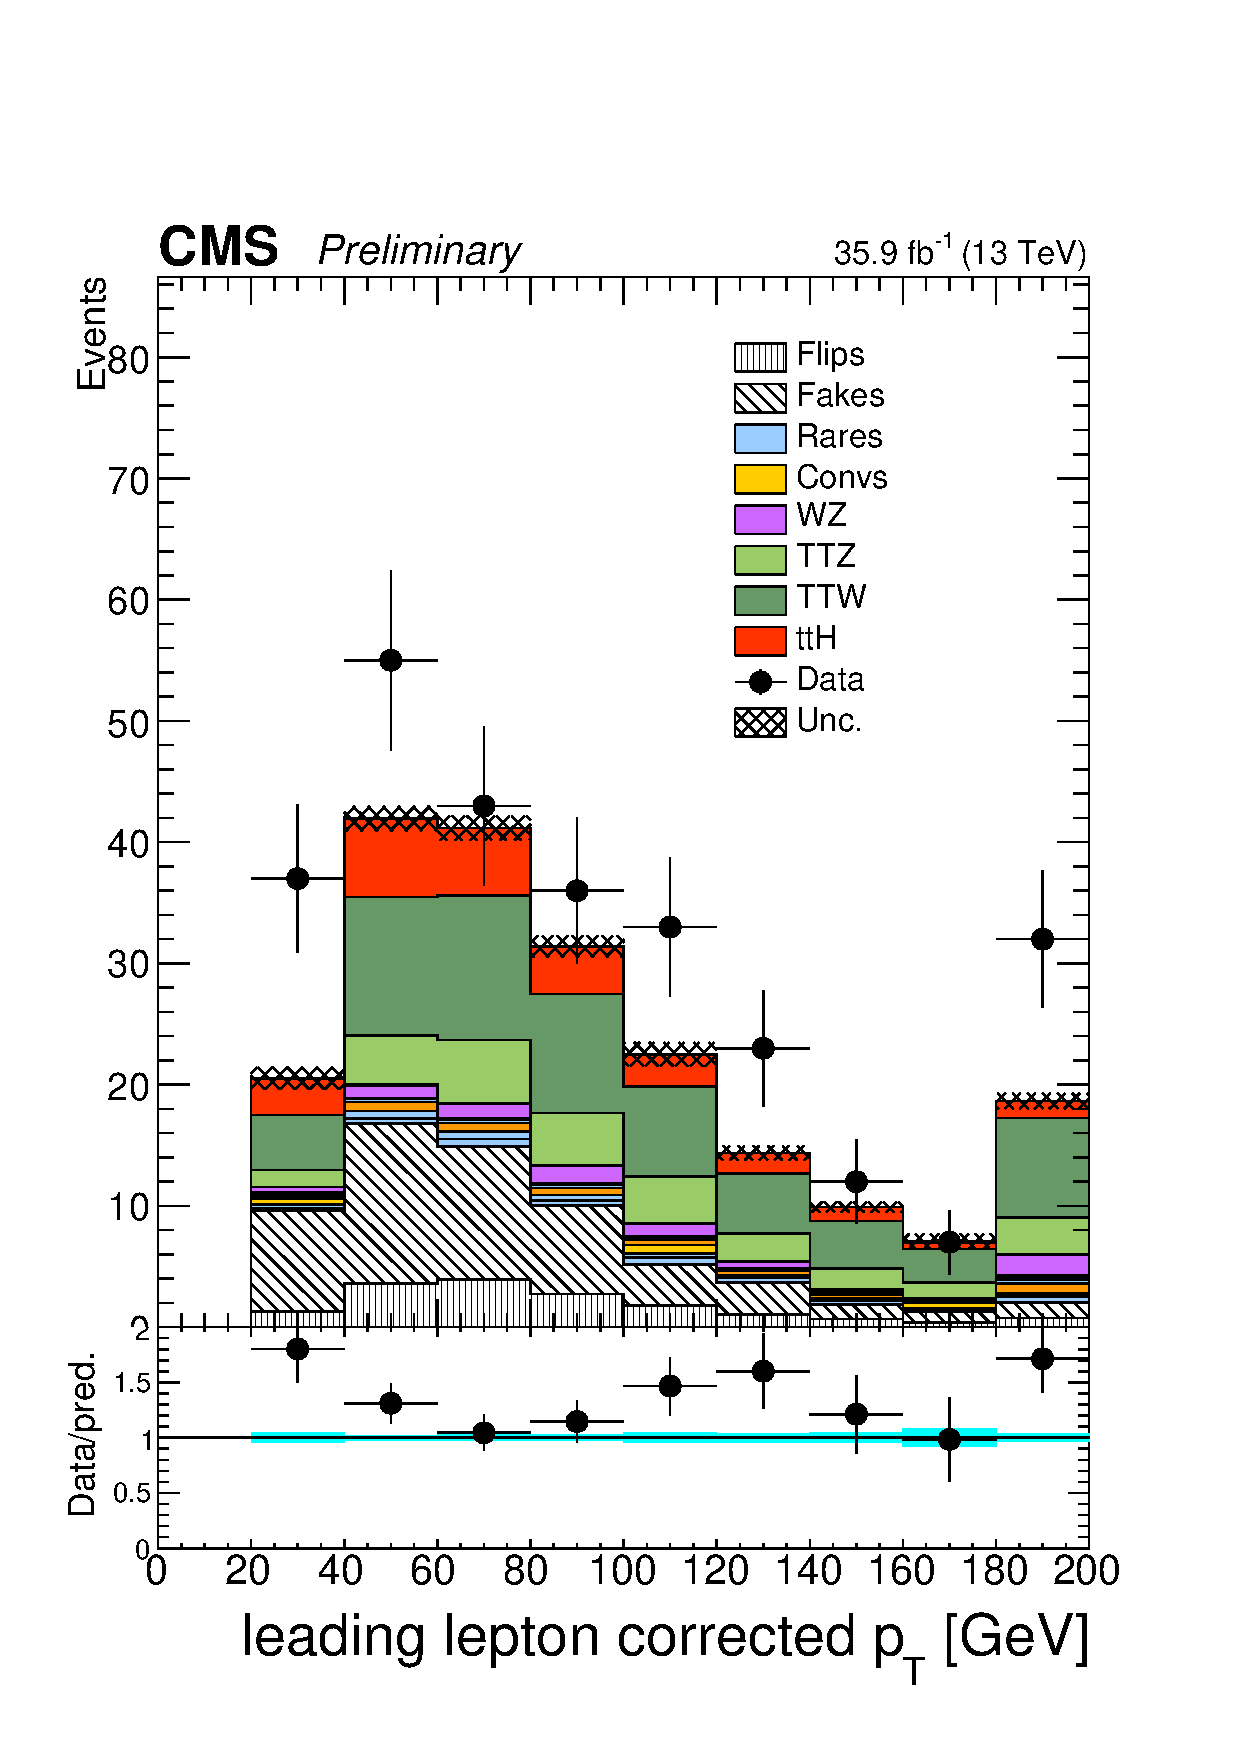
\includegraphics[width=0.32\textwidth]{ch5_figs/l1_pt_ttH_em_stackPlot_SR.pdf}
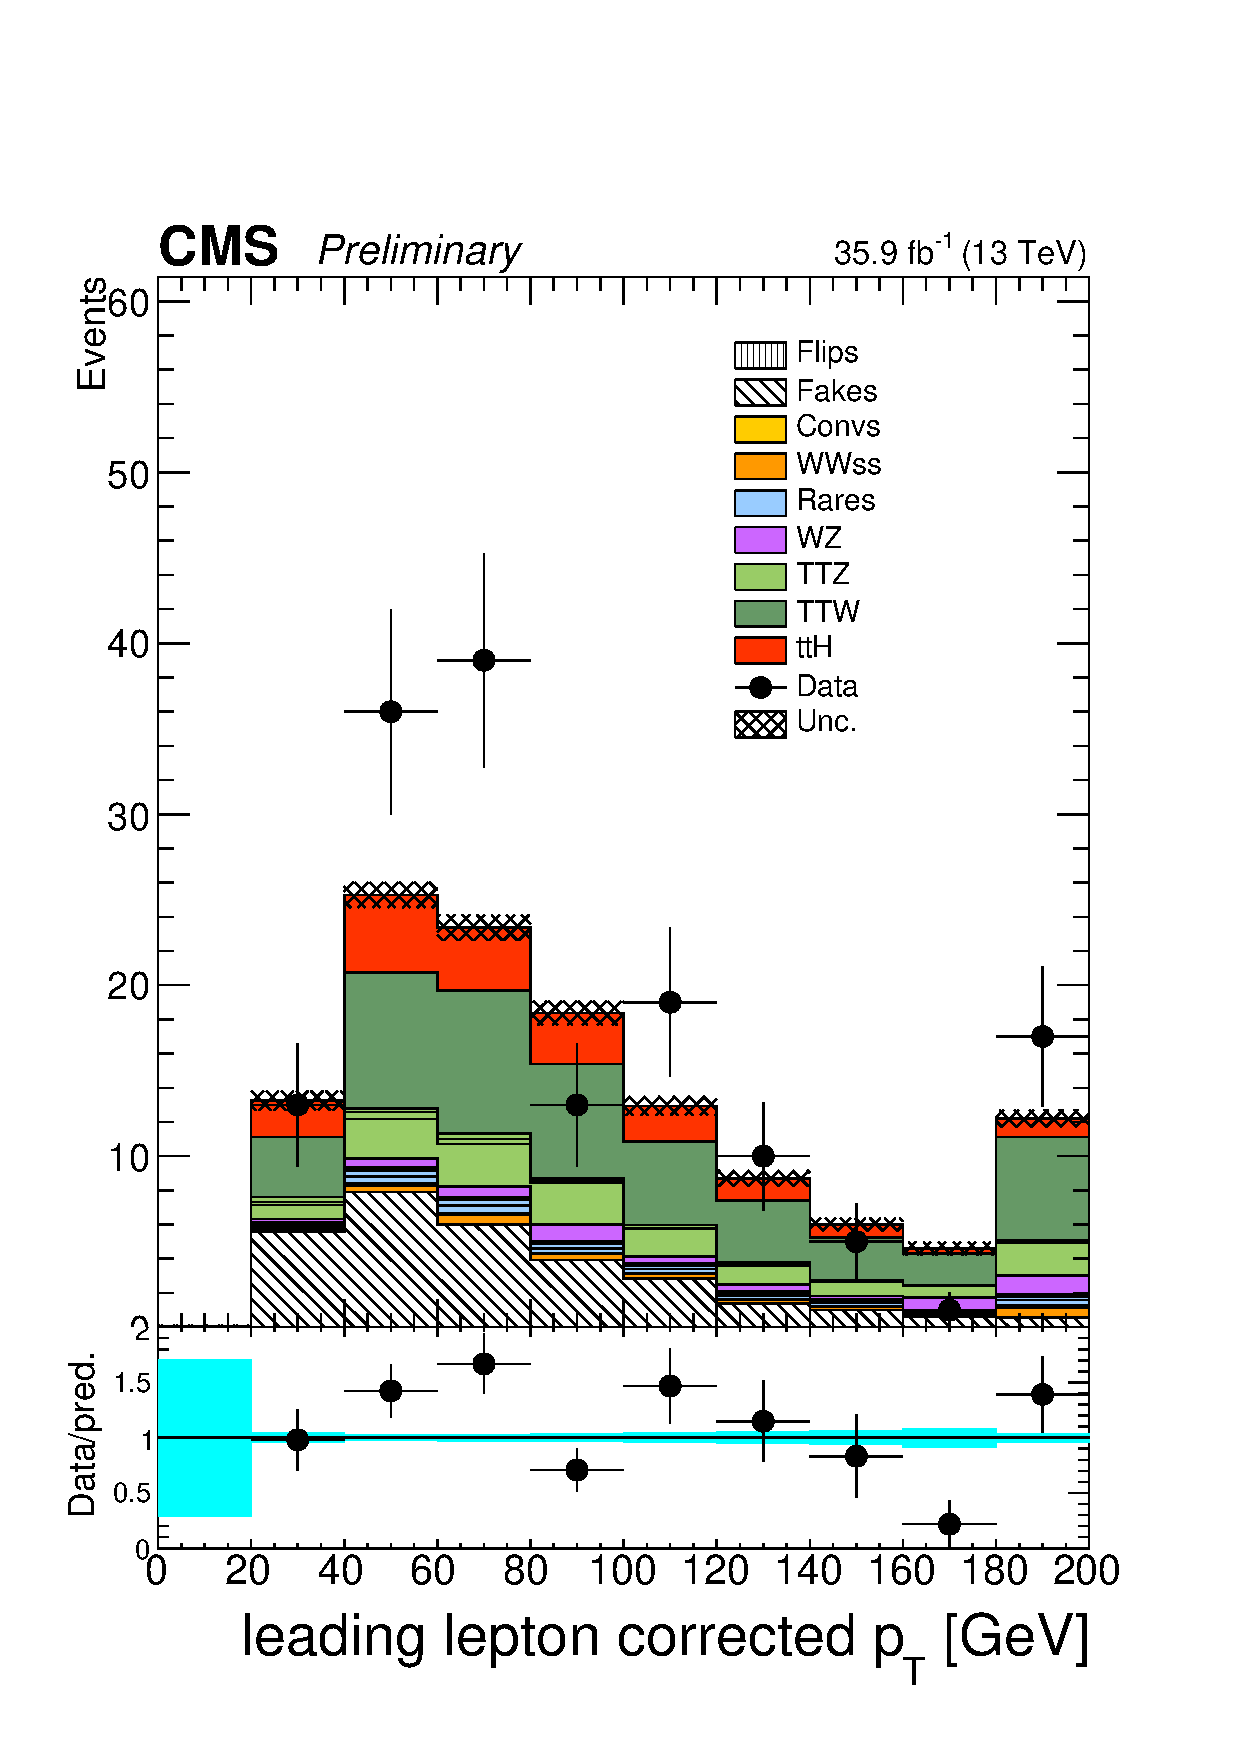
\includegraphics[width=0.32\textwidth]{ch5_figs/l1_pt_ttH_mm_stackPlot_SR.pdf} \\
\caption[Data/MC comparison of leading lepton \pt in the signal region]{The leading lepton transverse momenta in the 2lss $ee$/$e\mu$/$\mu\mu$ categories. Uncertainties shown are purely statistical.}
\label{fig:sr_l1pt}
\end{figure}

\begin{figure}[htp]
\centering
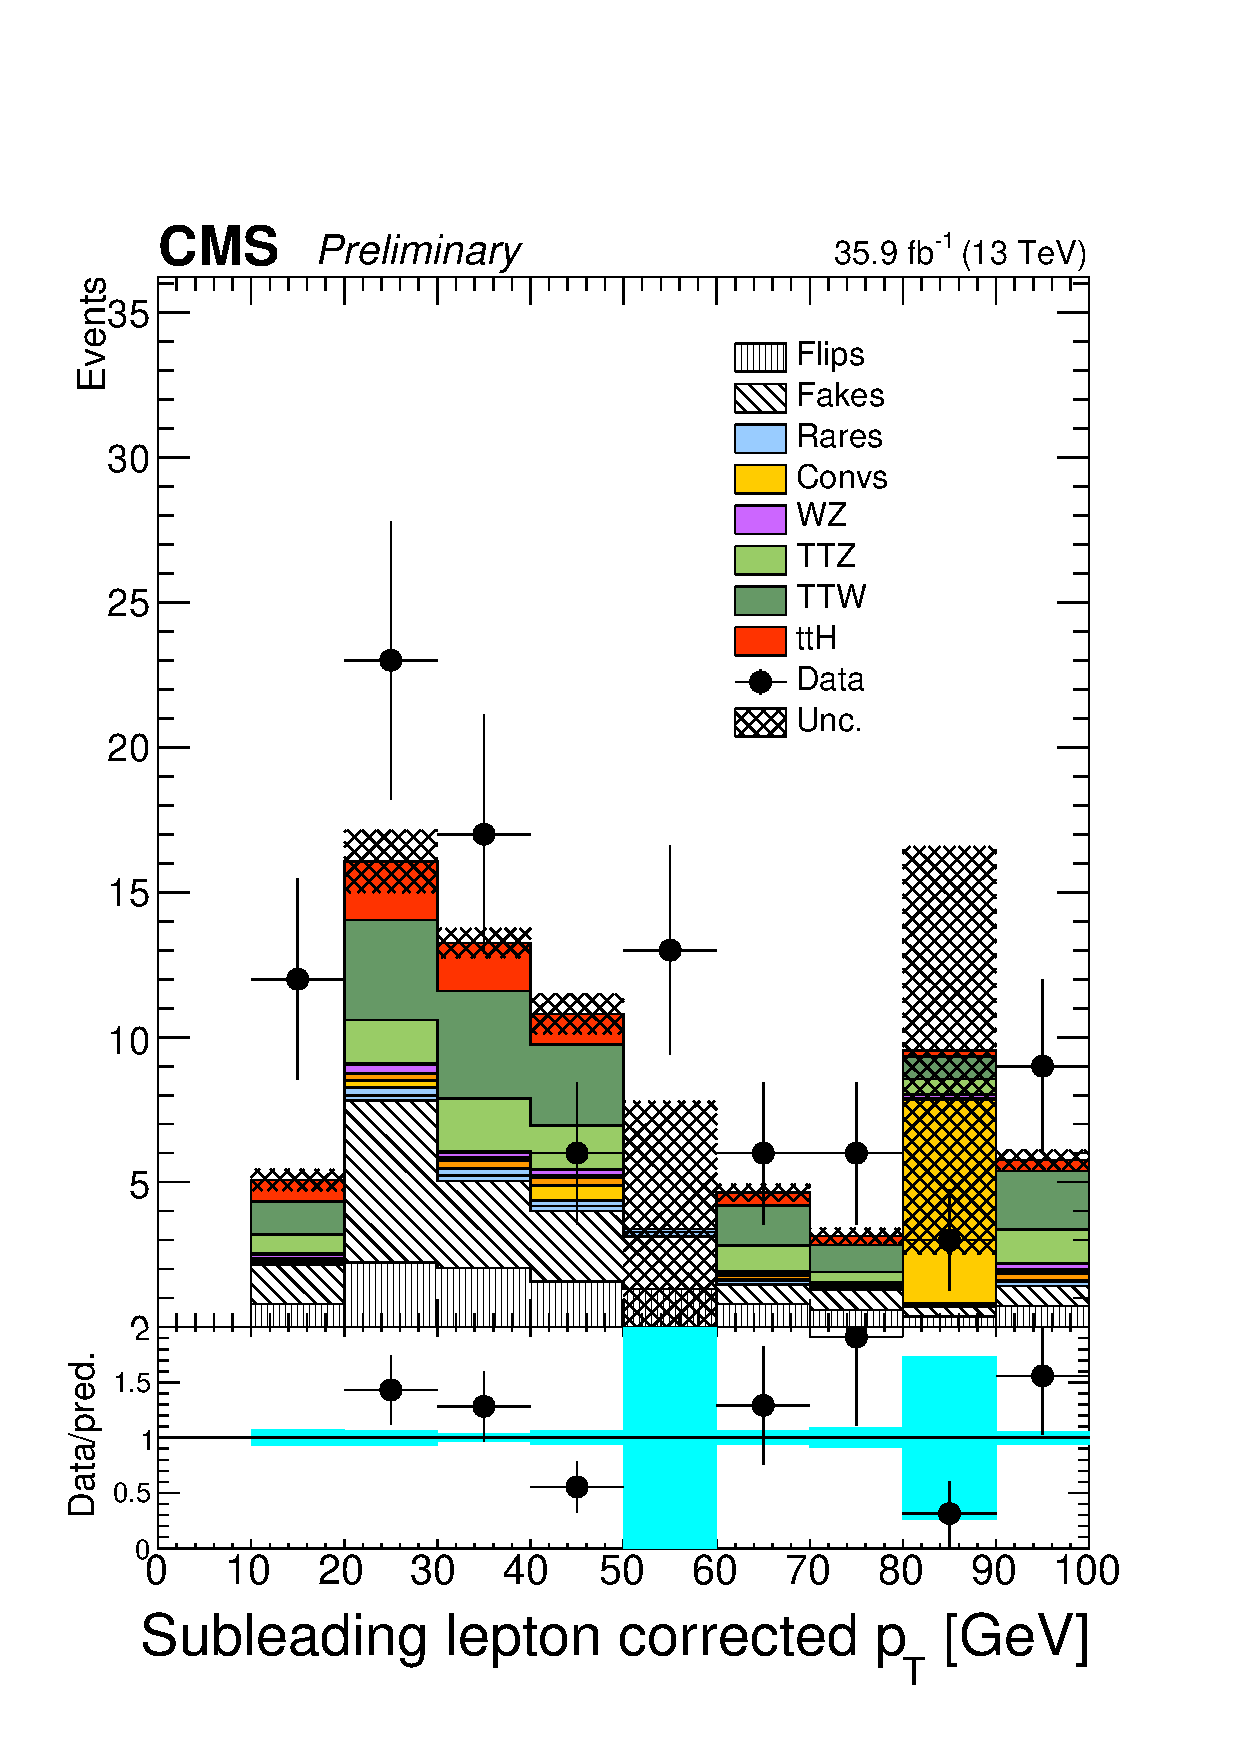
\includegraphics[width=0.32\textwidth]{ch5_figs/l2_pt_ttH_ee_stackPlot_SR.pdf}
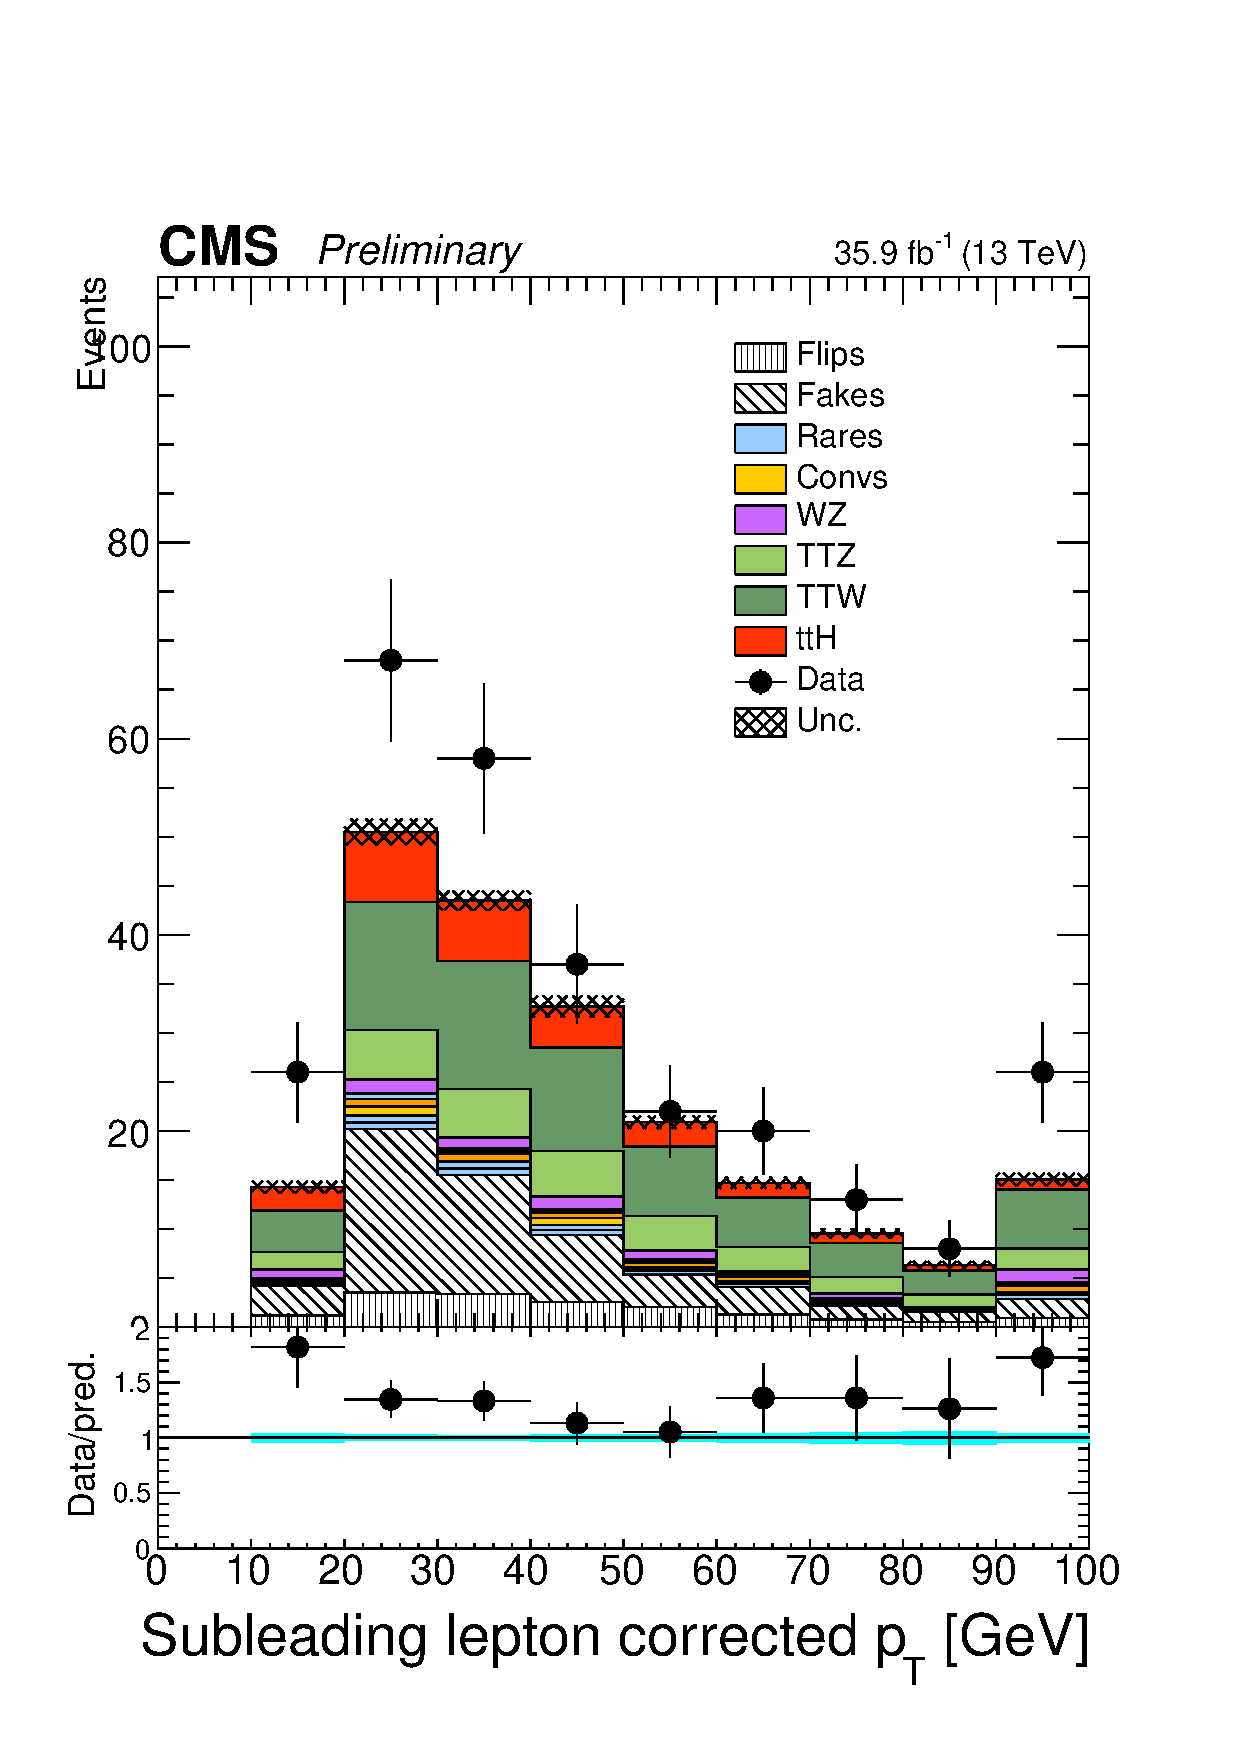
\includegraphics[width=0.32\textwidth]{ch5_figs/l2_pt_ttH_em_stackPlot_SR.pdf}
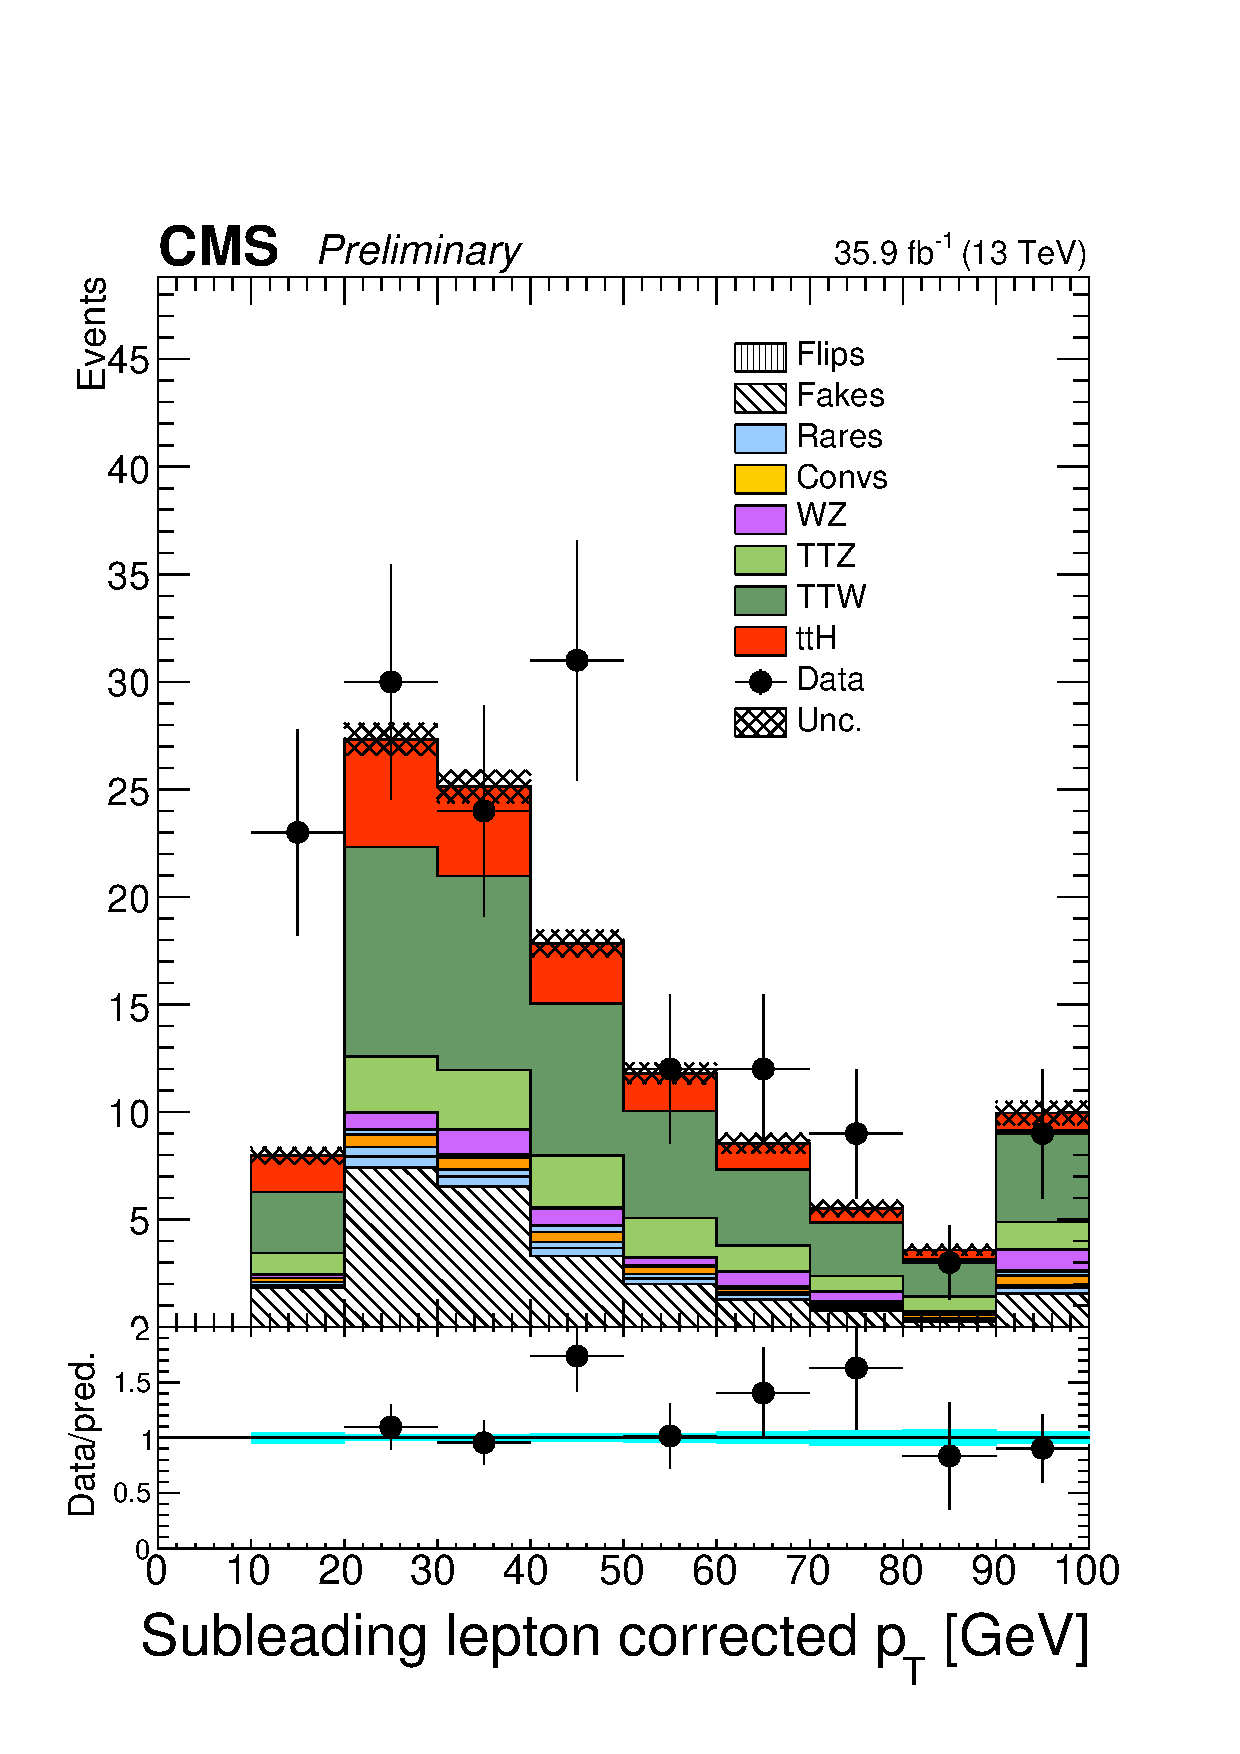
\includegraphics[width=0.32\textwidth]{ch5_figs/l2_pt_ttH_mm_stackPlot_SR.pdf} \\
\caption[Data/MC comparison of subleading lepton \pt in the signal region]{The sub leading lepton transverse momenta in the 2lss $ee$/$e\mu$/$\mu\mu$ categories. Uncertainties shown are purely statistical.}
\label{fig:sr_l2pt}
\end{figure}

\begin{figure}[htp]
\centering
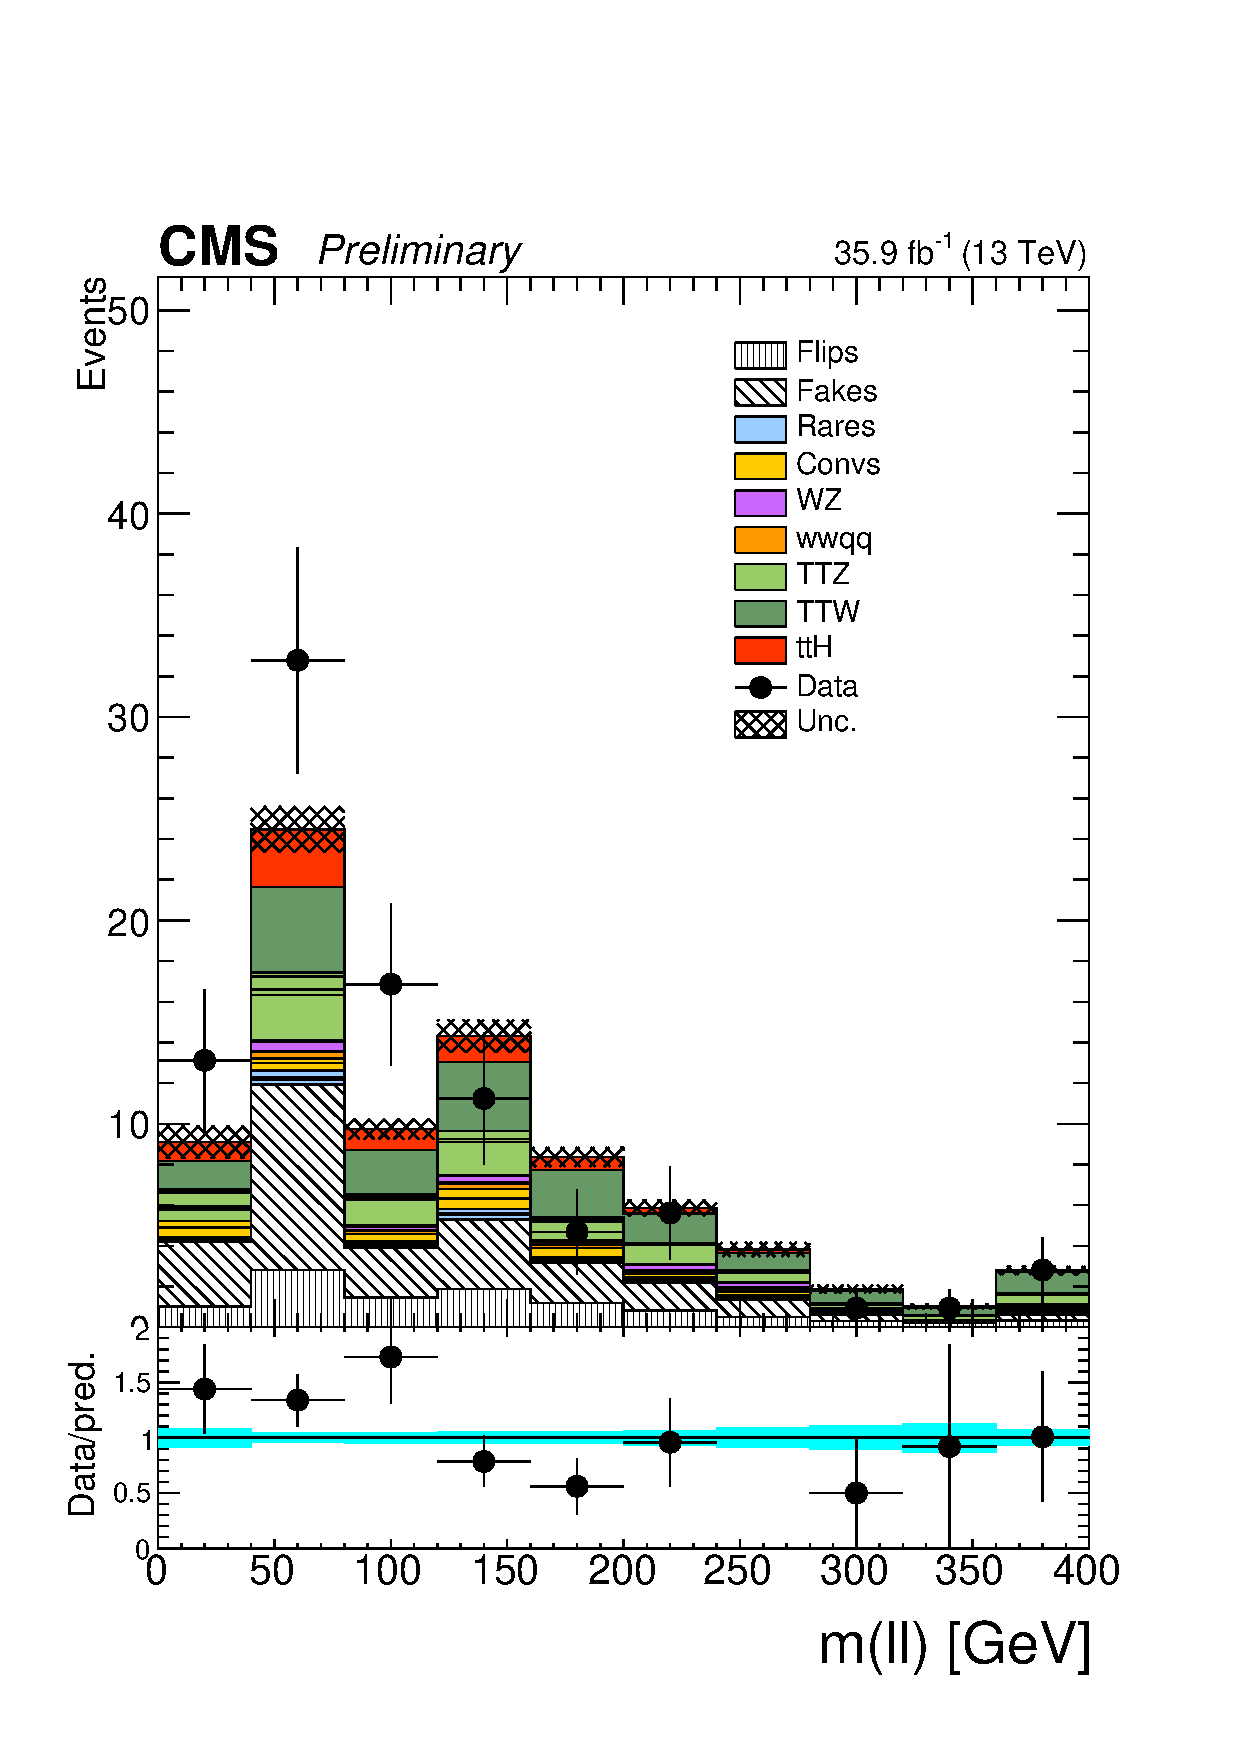
\includegraphics[width=0.32\textwidth]{ch5_figs/mll_ttH_ee_stackPlot_SR.pdf}
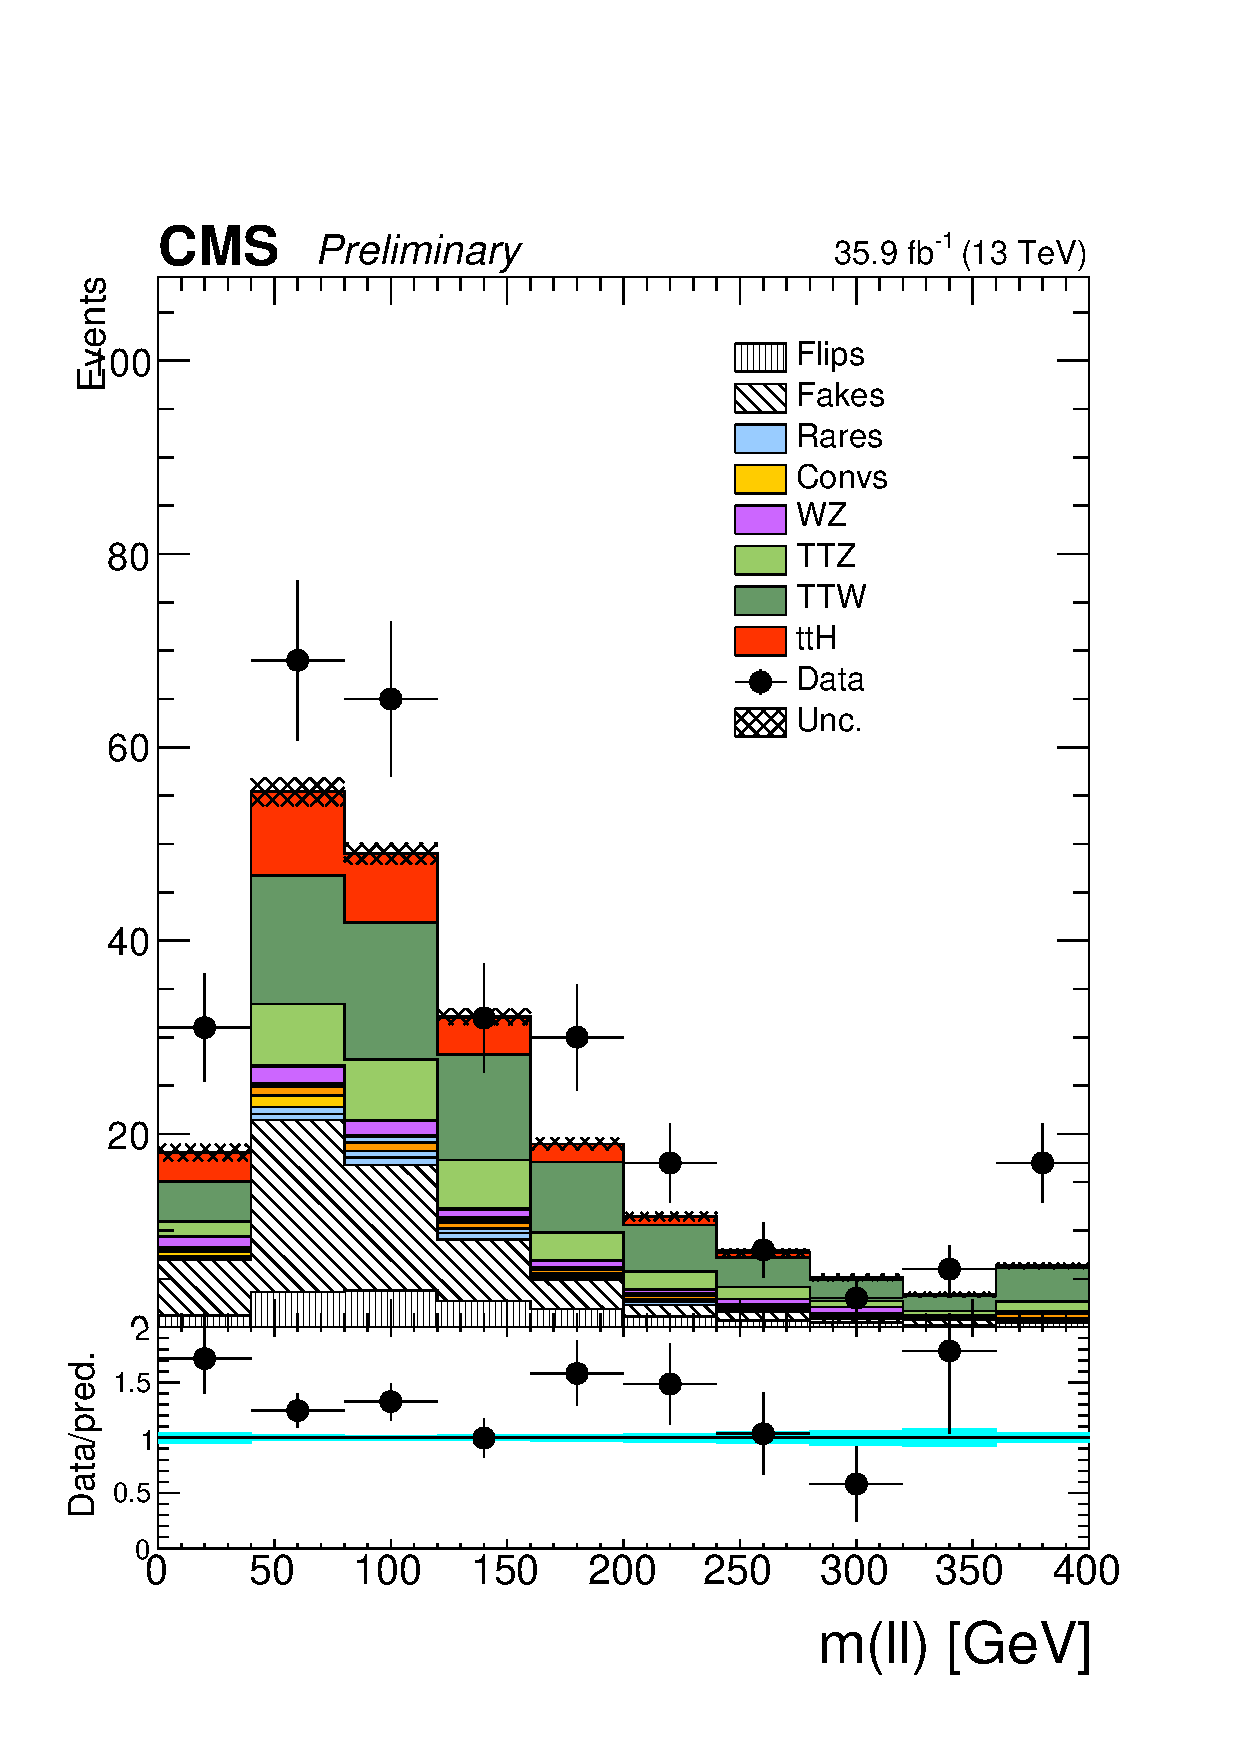
\includegraphics[width=0.32\textwidth]{ch5_figs/mll_ttH_em_stackPlot_SR.pdf}
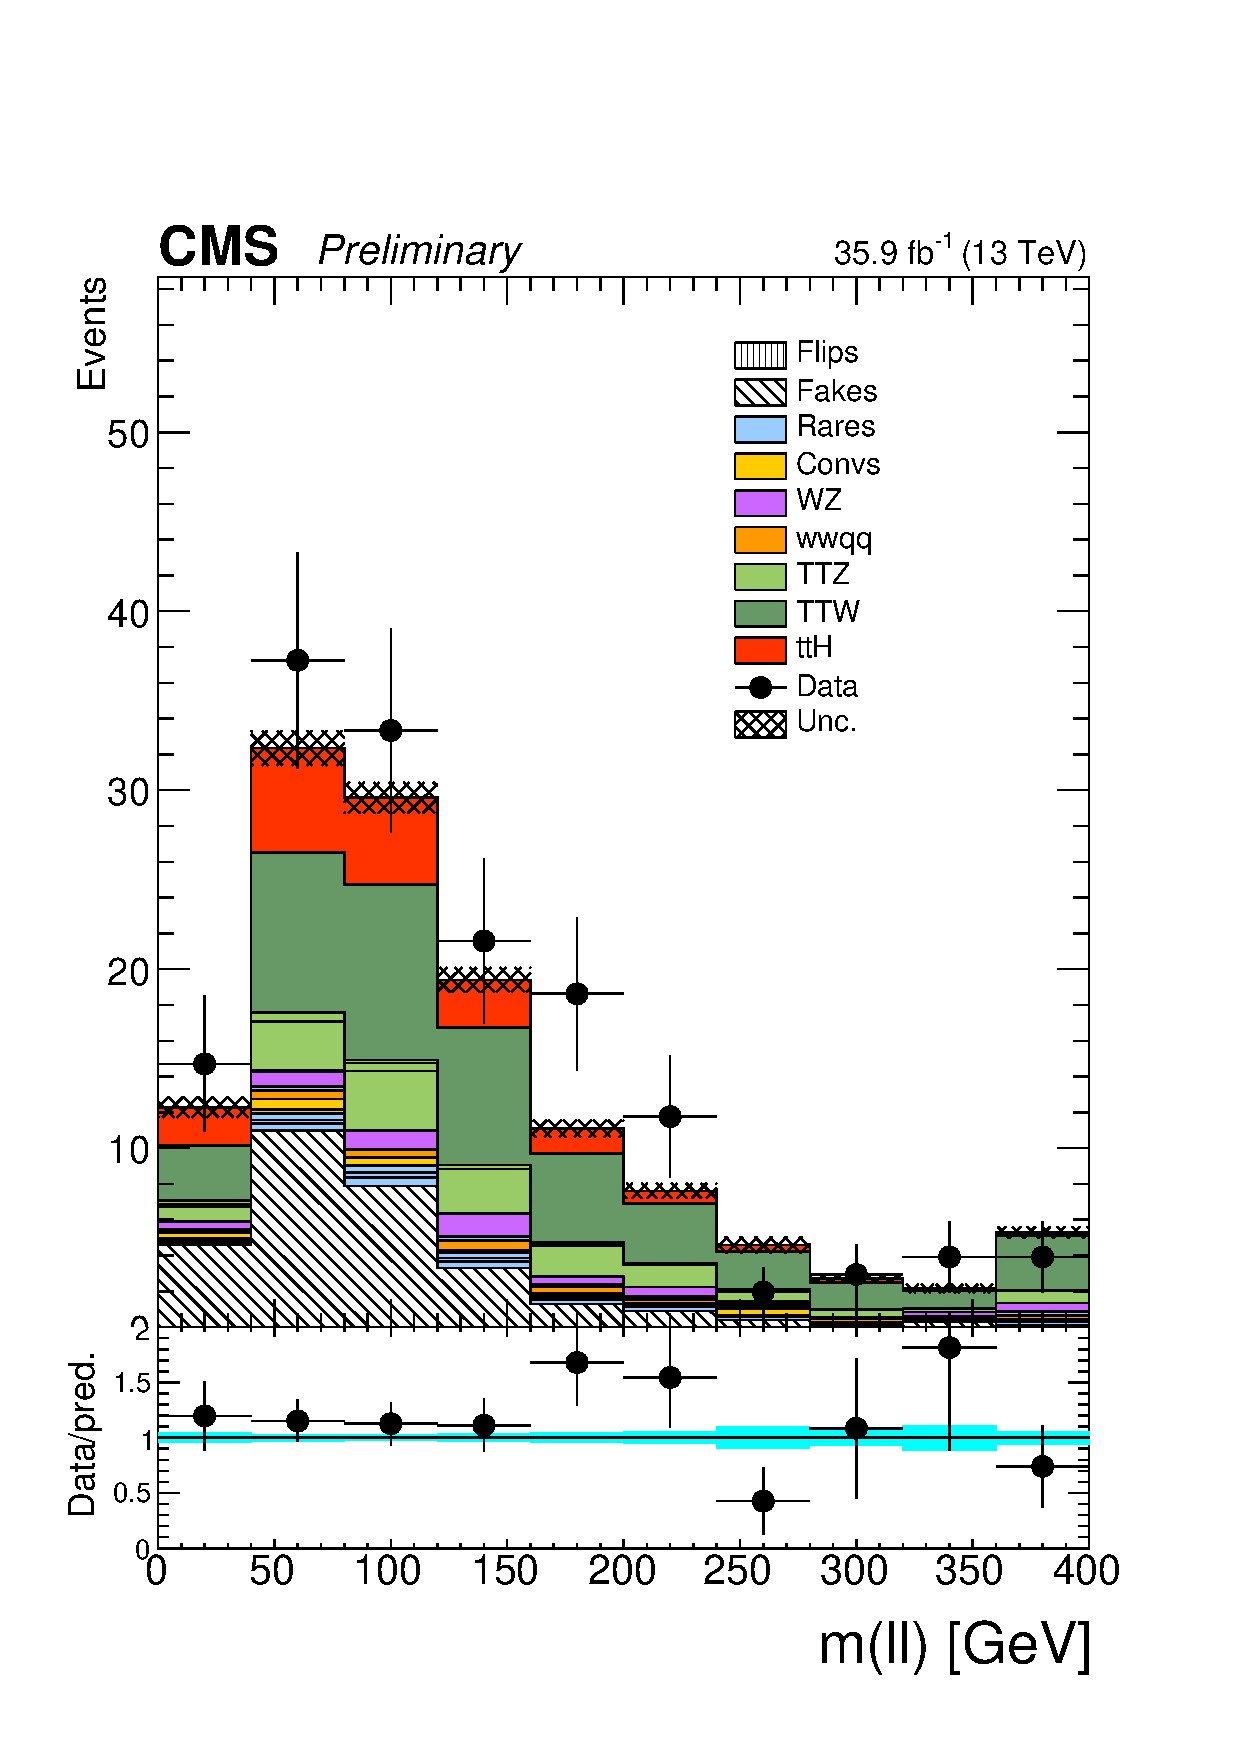
\includegraphics[width=0.32\textwidth]{ch5_figs/mll_ttH_mm_stackPlot_SR.pdf} \\
\caption[Data/MC comparison of dilepton invariant mass spectra in the signal region]{The dilepton invariant mass spectra in the 2lss $ee$/$e\mu$/$\mu\mu$ categories. Uncertainties shown are purely statistical.}
\label{fig:sr_mll}
\end{figure}

\begin{figure}[htp]
\centering
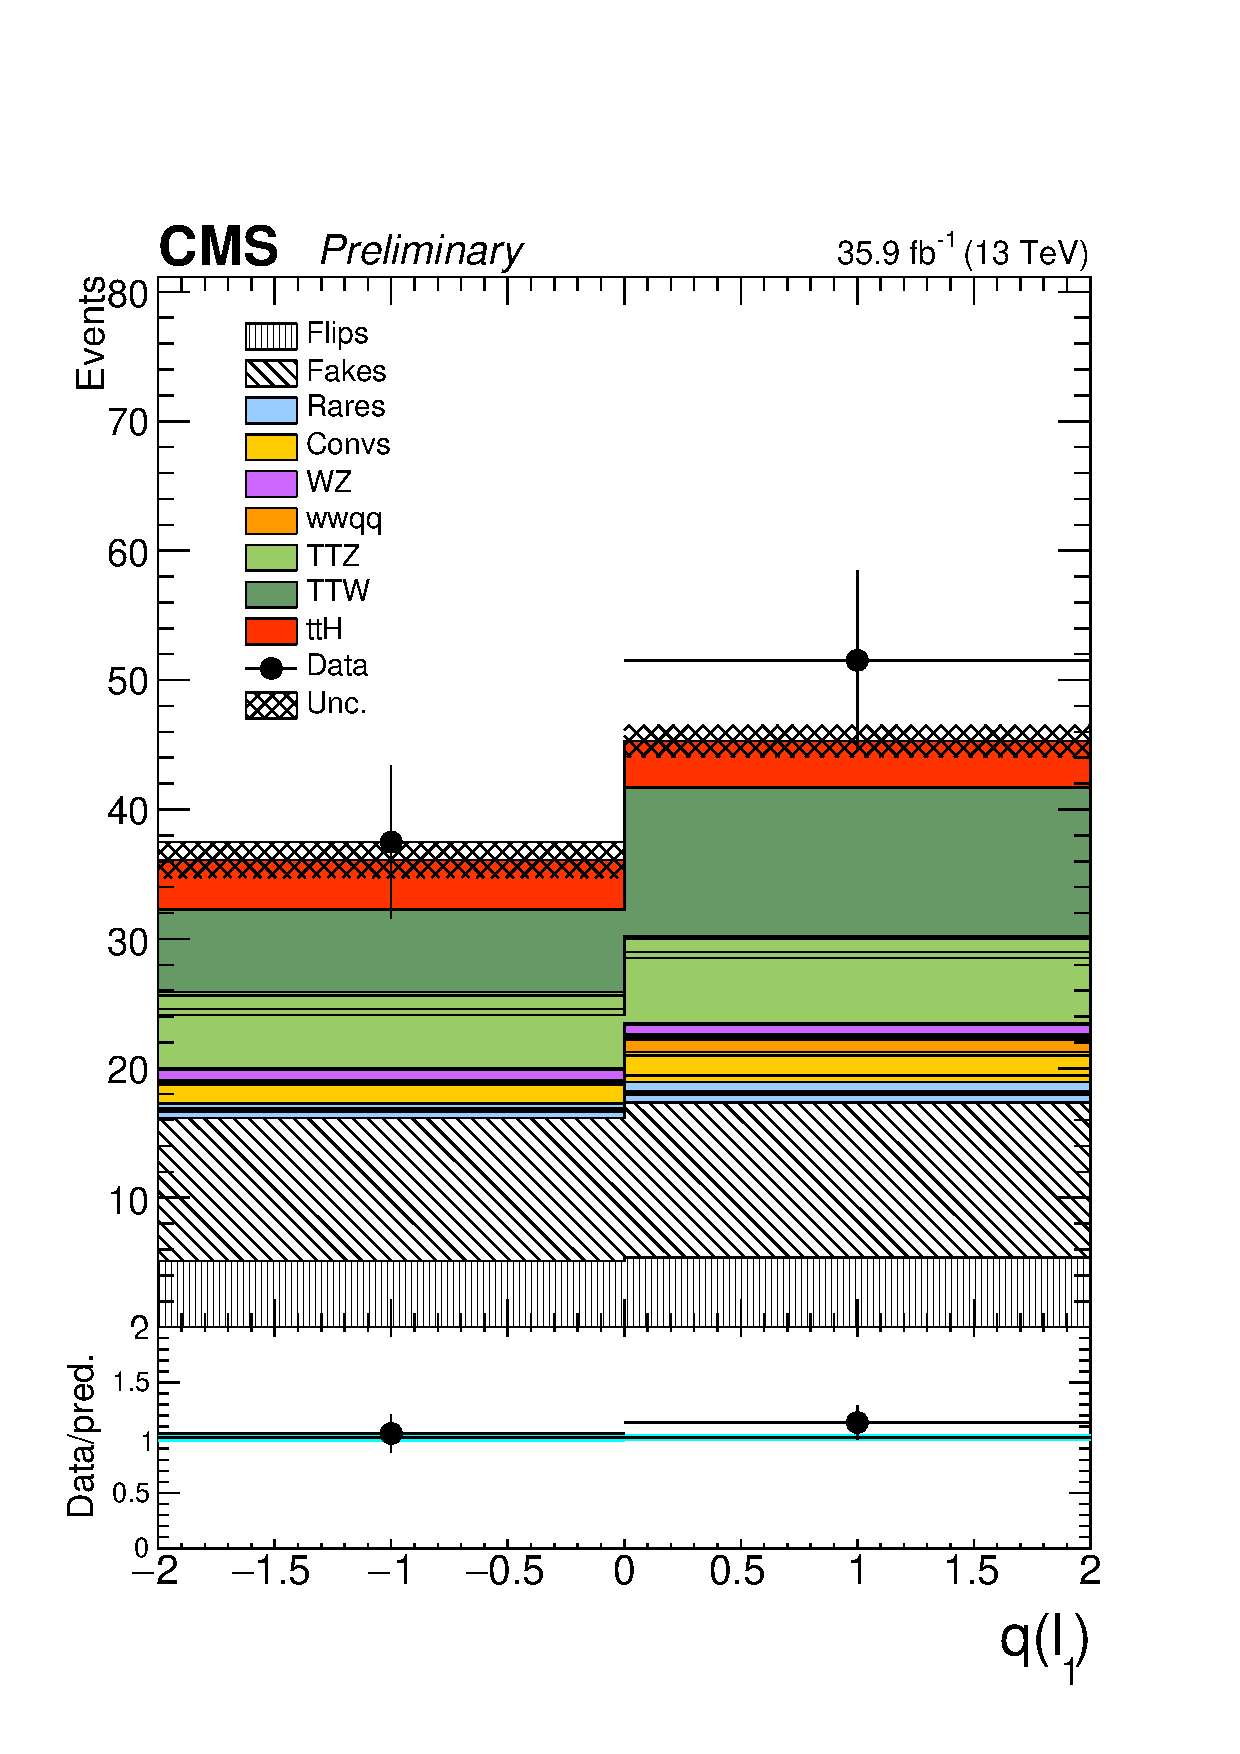
\includegraphics[width=0.32\textwidth]{ch5_figs/qSum_ttH_ee_stackPlot_SR.pdf}
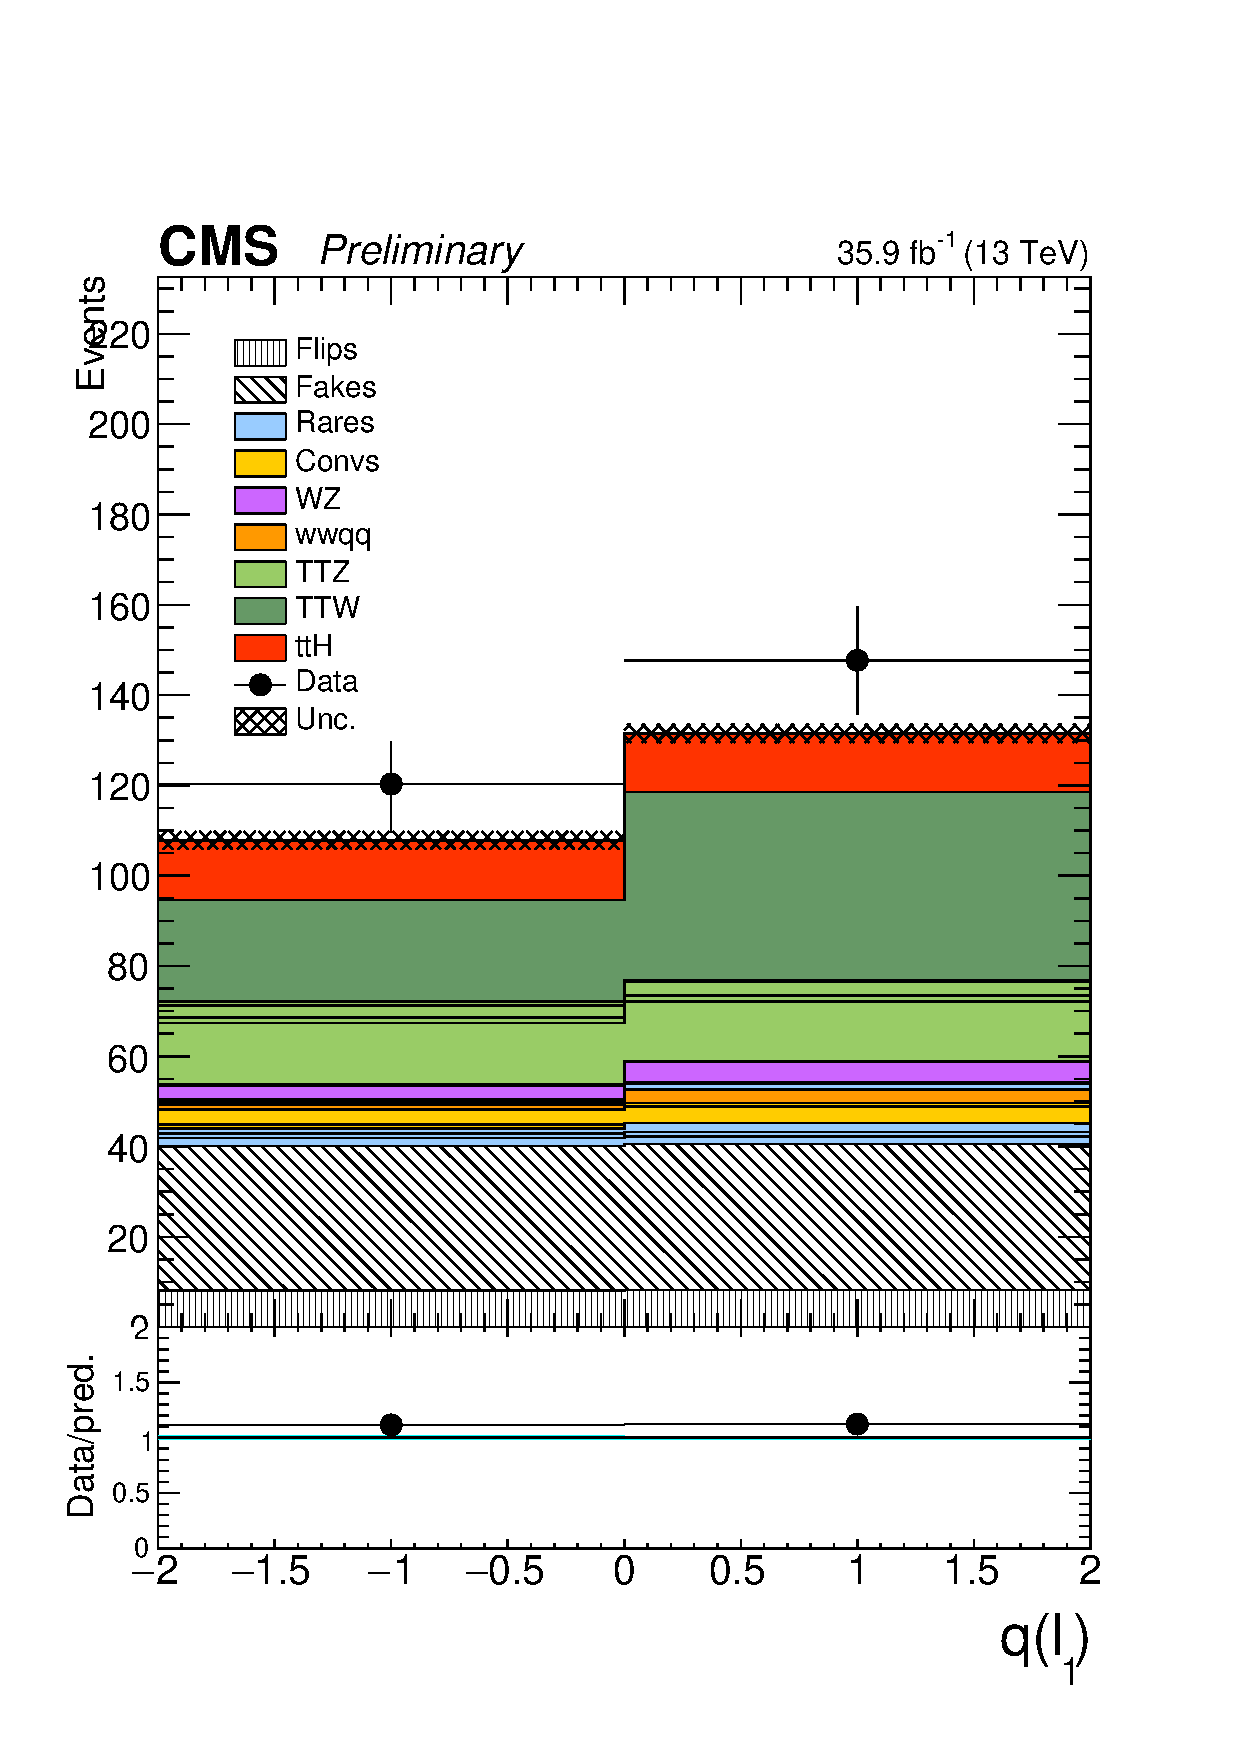
\includegraphics[width=0.32\textwidth]{ch5_figs/qSum_ttH_em_stackPlot_SR.pdf}
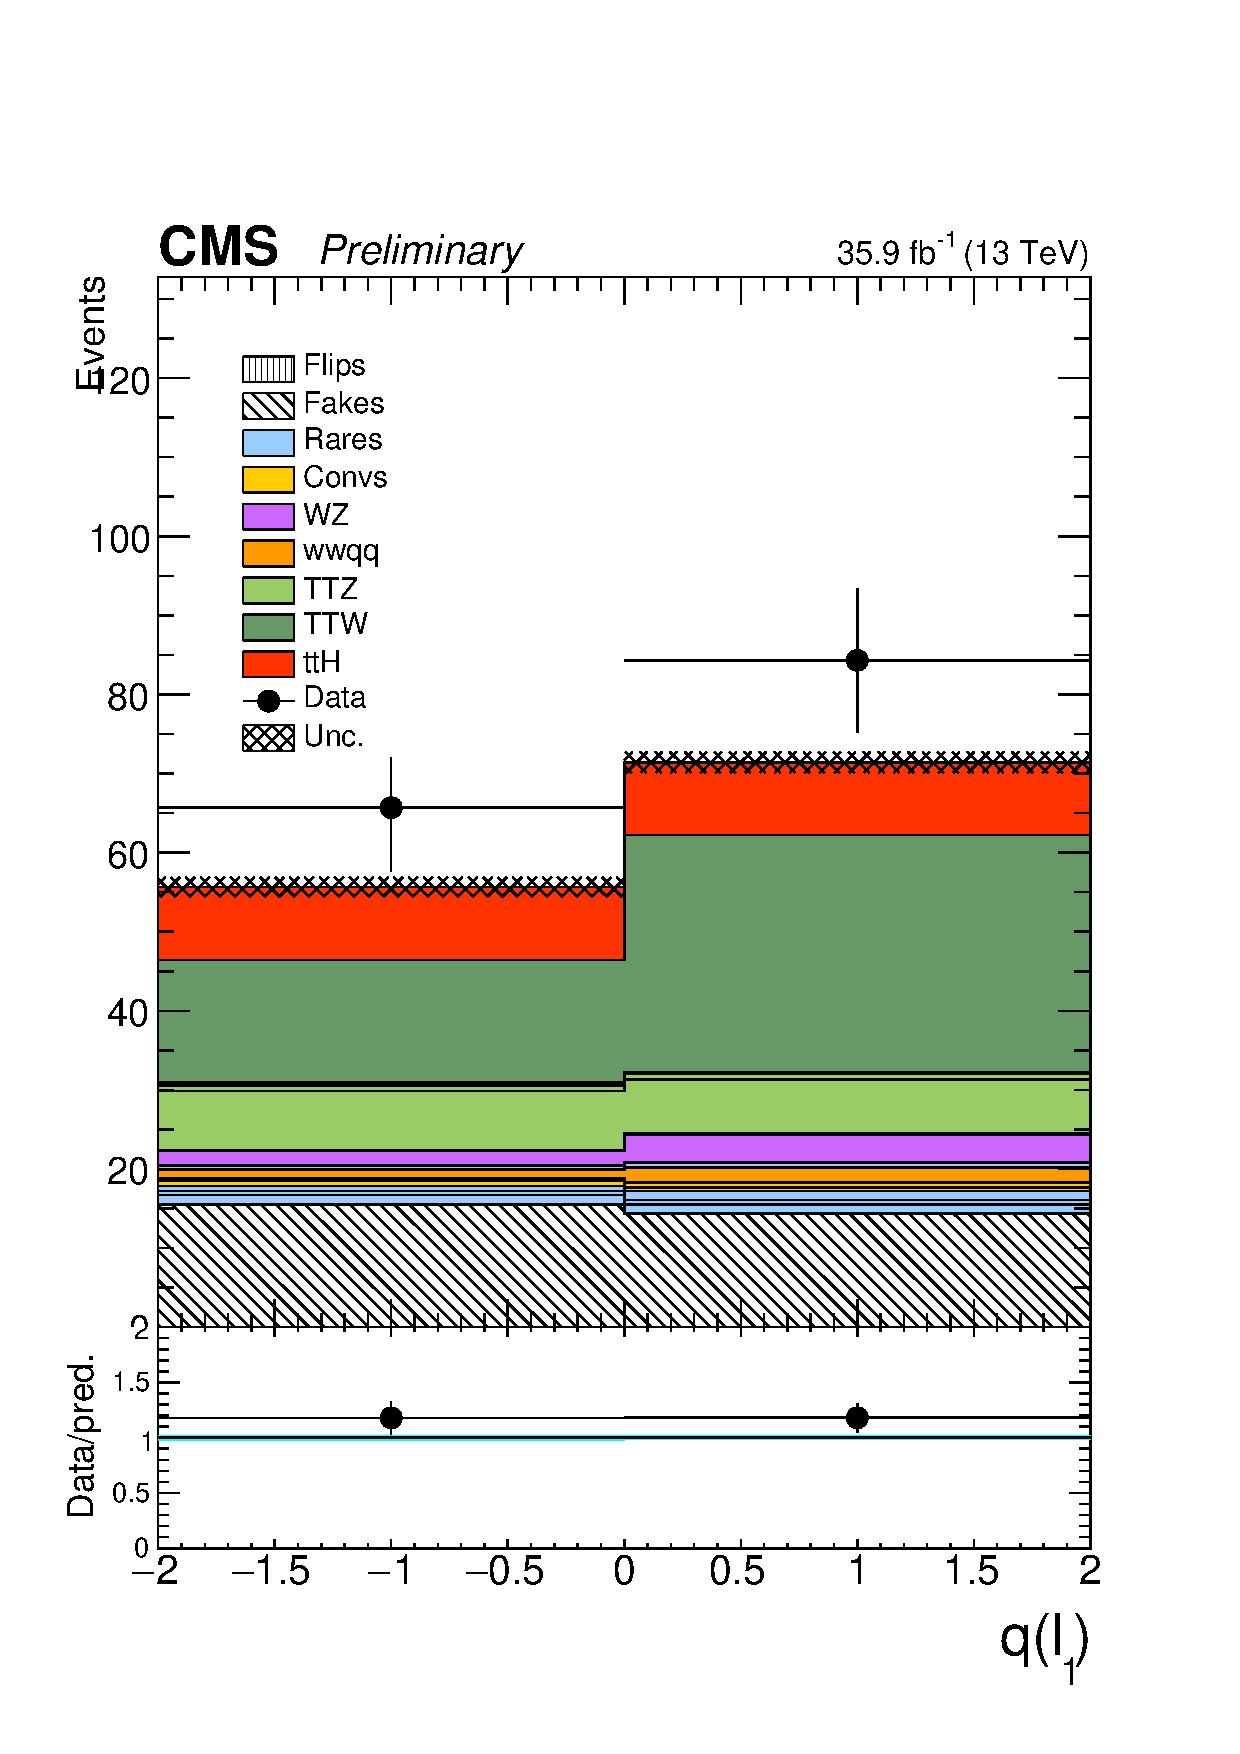
\includegraphics[width=0.32\textwidth]{ch5_figs/qSum_ttH_mm_stackPlot_SR.pdf} \\
\caption[Data/MC comparison of sum of the lepton electric charges in the signal region]{The sum of the lepton electric charges in the 2lss $ee$/$e\mu$/$\mu\mu$ categories. Uncertainties shown are purely statistical.}
\label{fig:sr_qsum}
\end{figure}

\begin{figure}[htp]
\centering
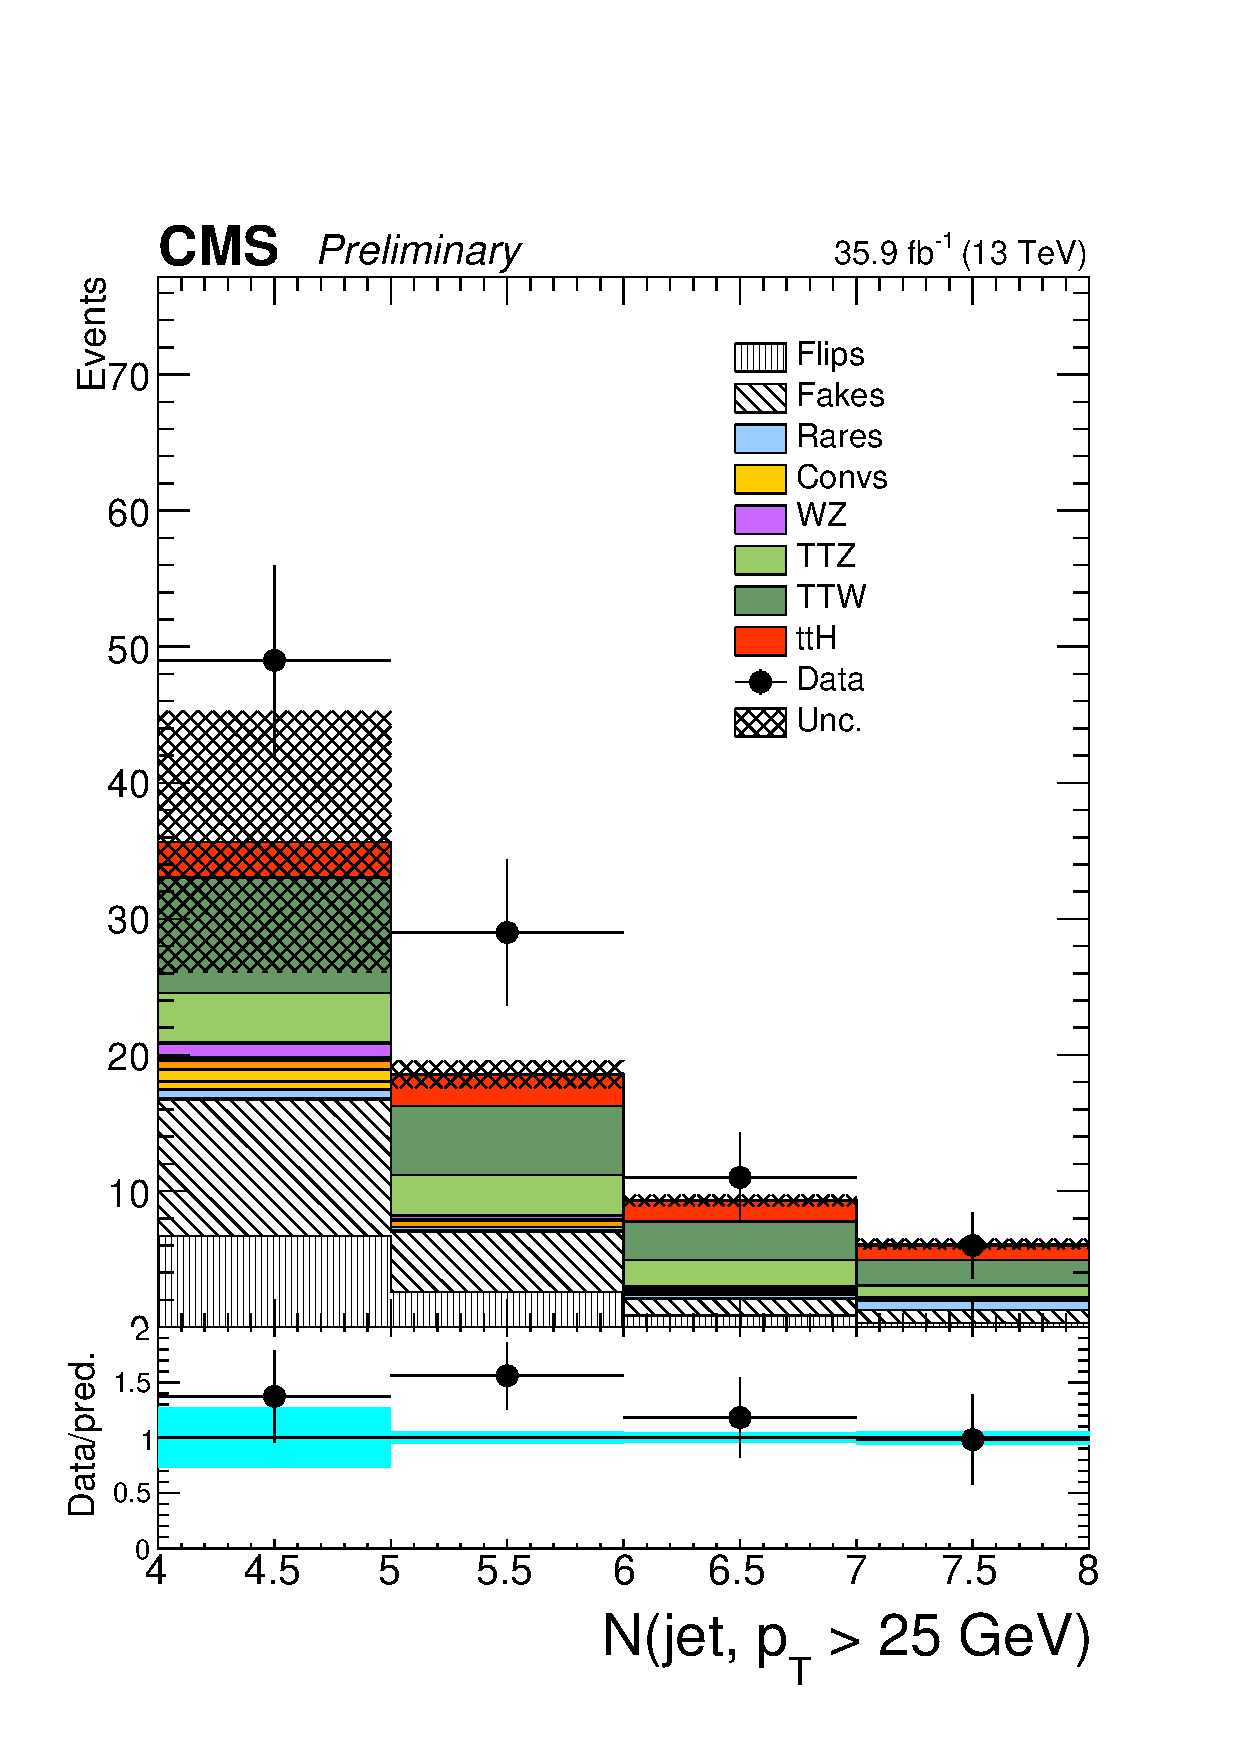
\includegraphics[width=0.32\textwidth]{ch5_figs/nJets_ttH_ee_stackPlot_SR.pdf}
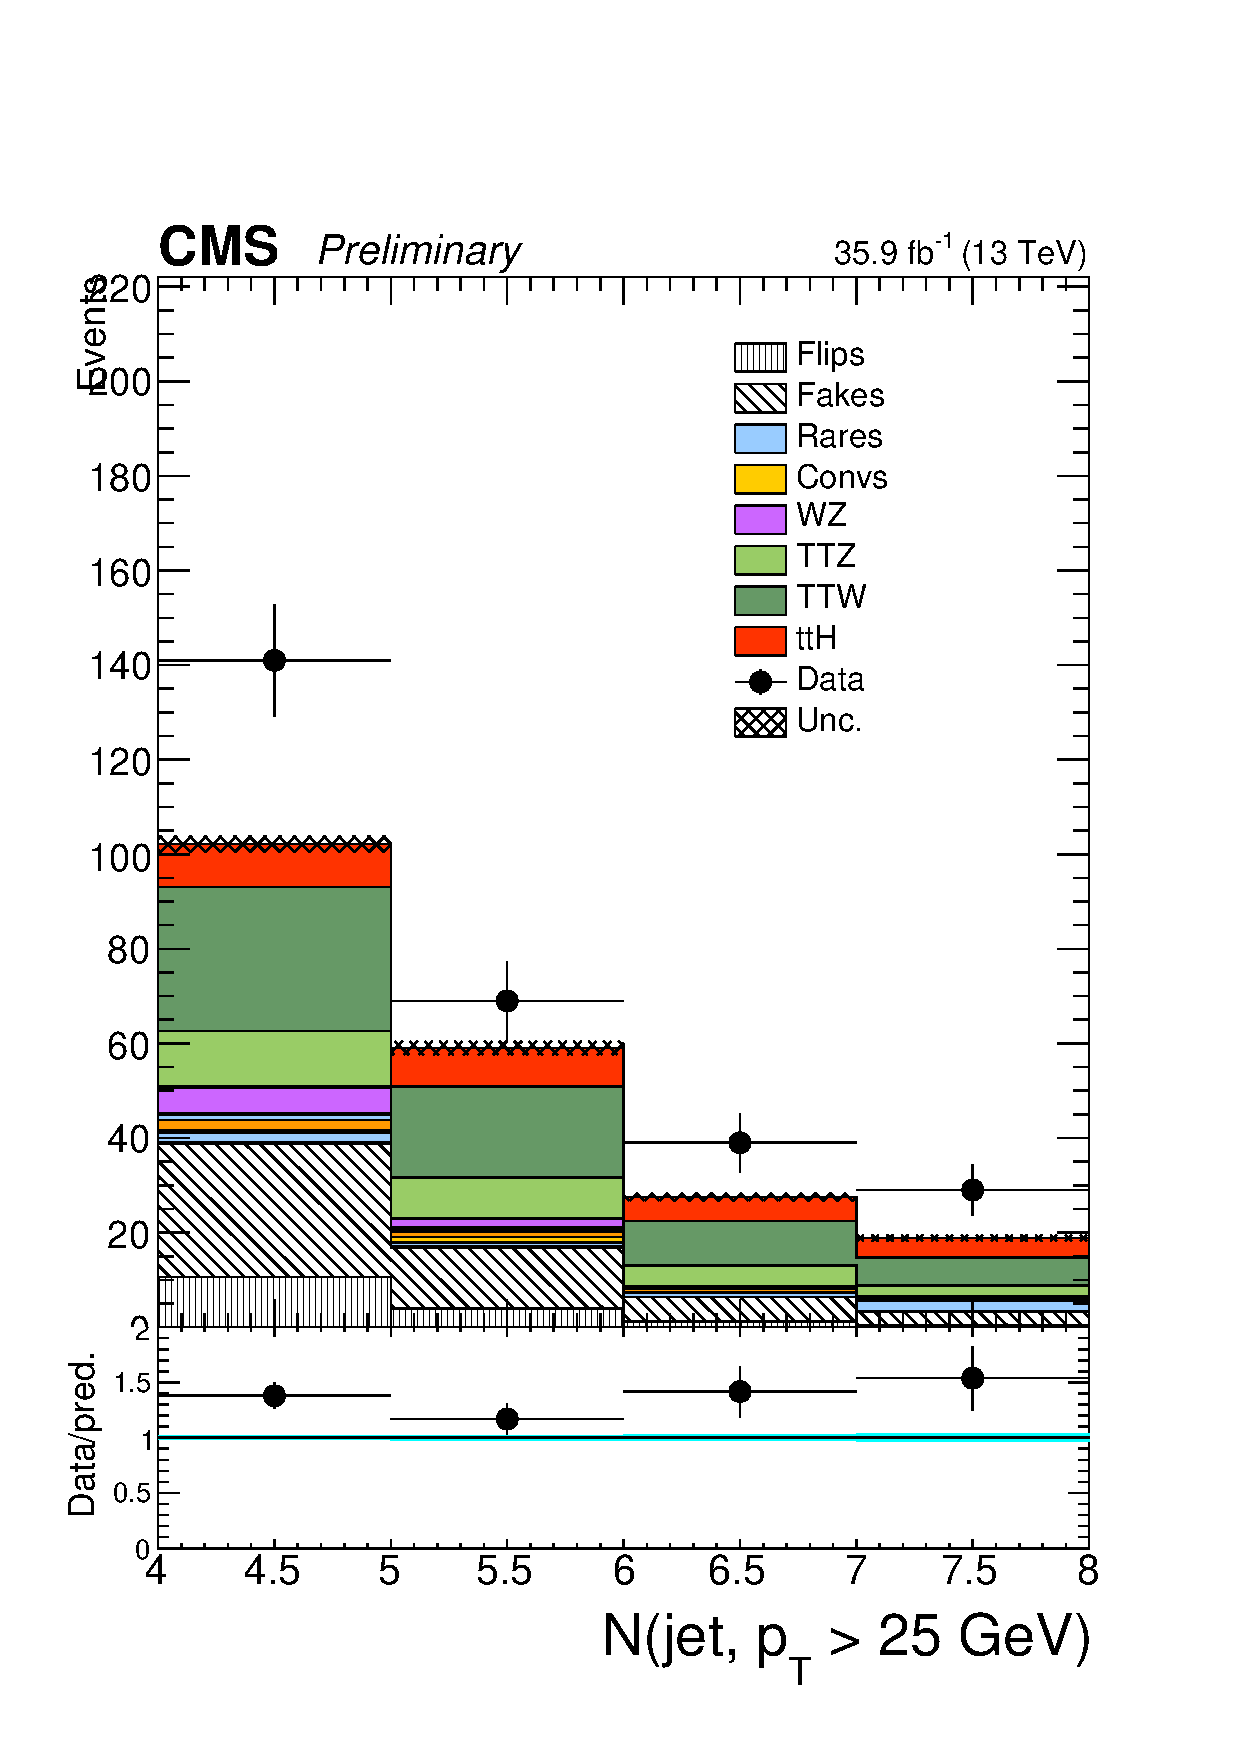
\includegraphics[width=0.32\textwidth]{ch5_figs/nJets_ttH_em_stackPlot_SR.pdf}
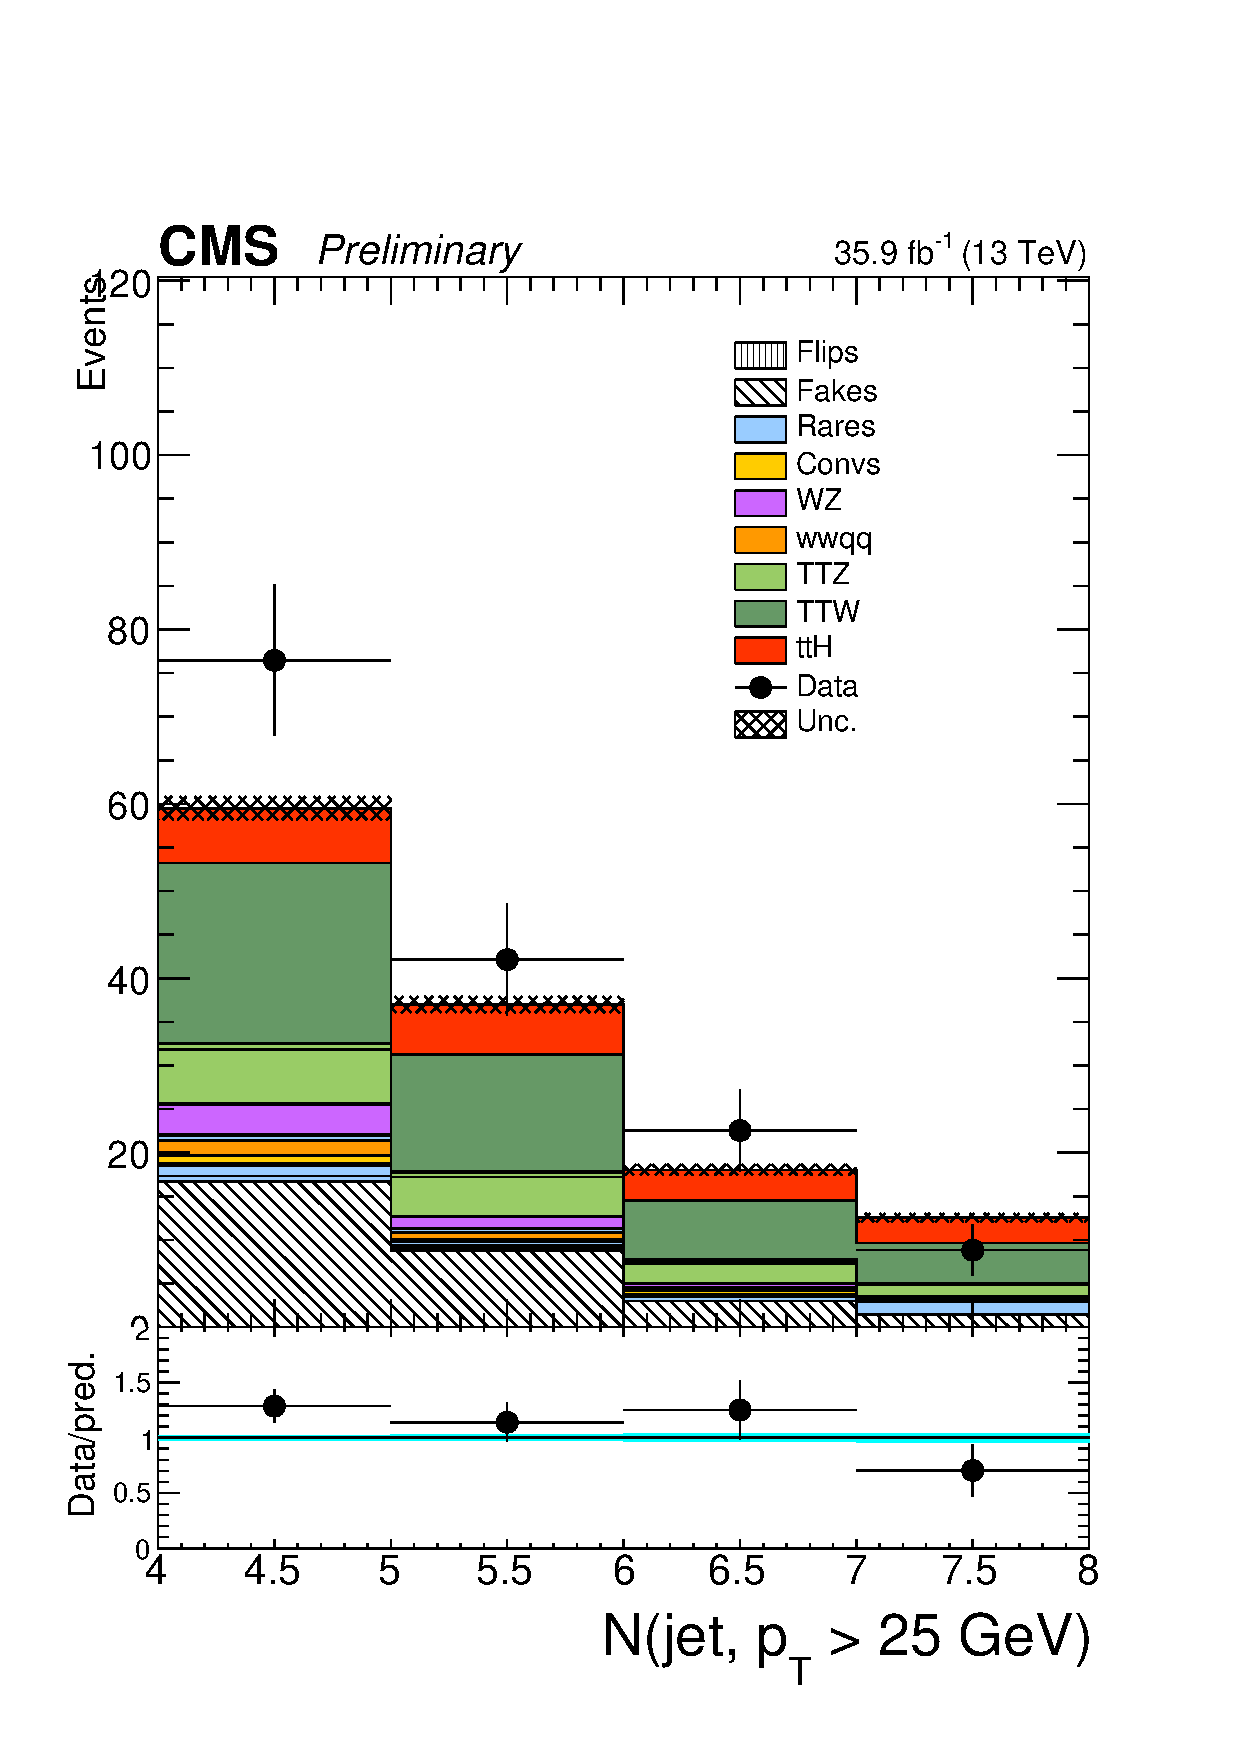
\includegraphics[width=0.32\textwidth]{ch5_figs/nJets_ttH_mm_stackPlot_SR.pdf} \\
\caption[Data/MC comparison of the jet multiplicity in the signal region]{The jet multiplicity distribution in the 2lss $ee$/$e\mu$/$\mu\mu$ categories. Uncertainties shown are purely statistical.}
\label{fig:sr_njets}
\end{figure}

\begin{figure}[htp]
\centering
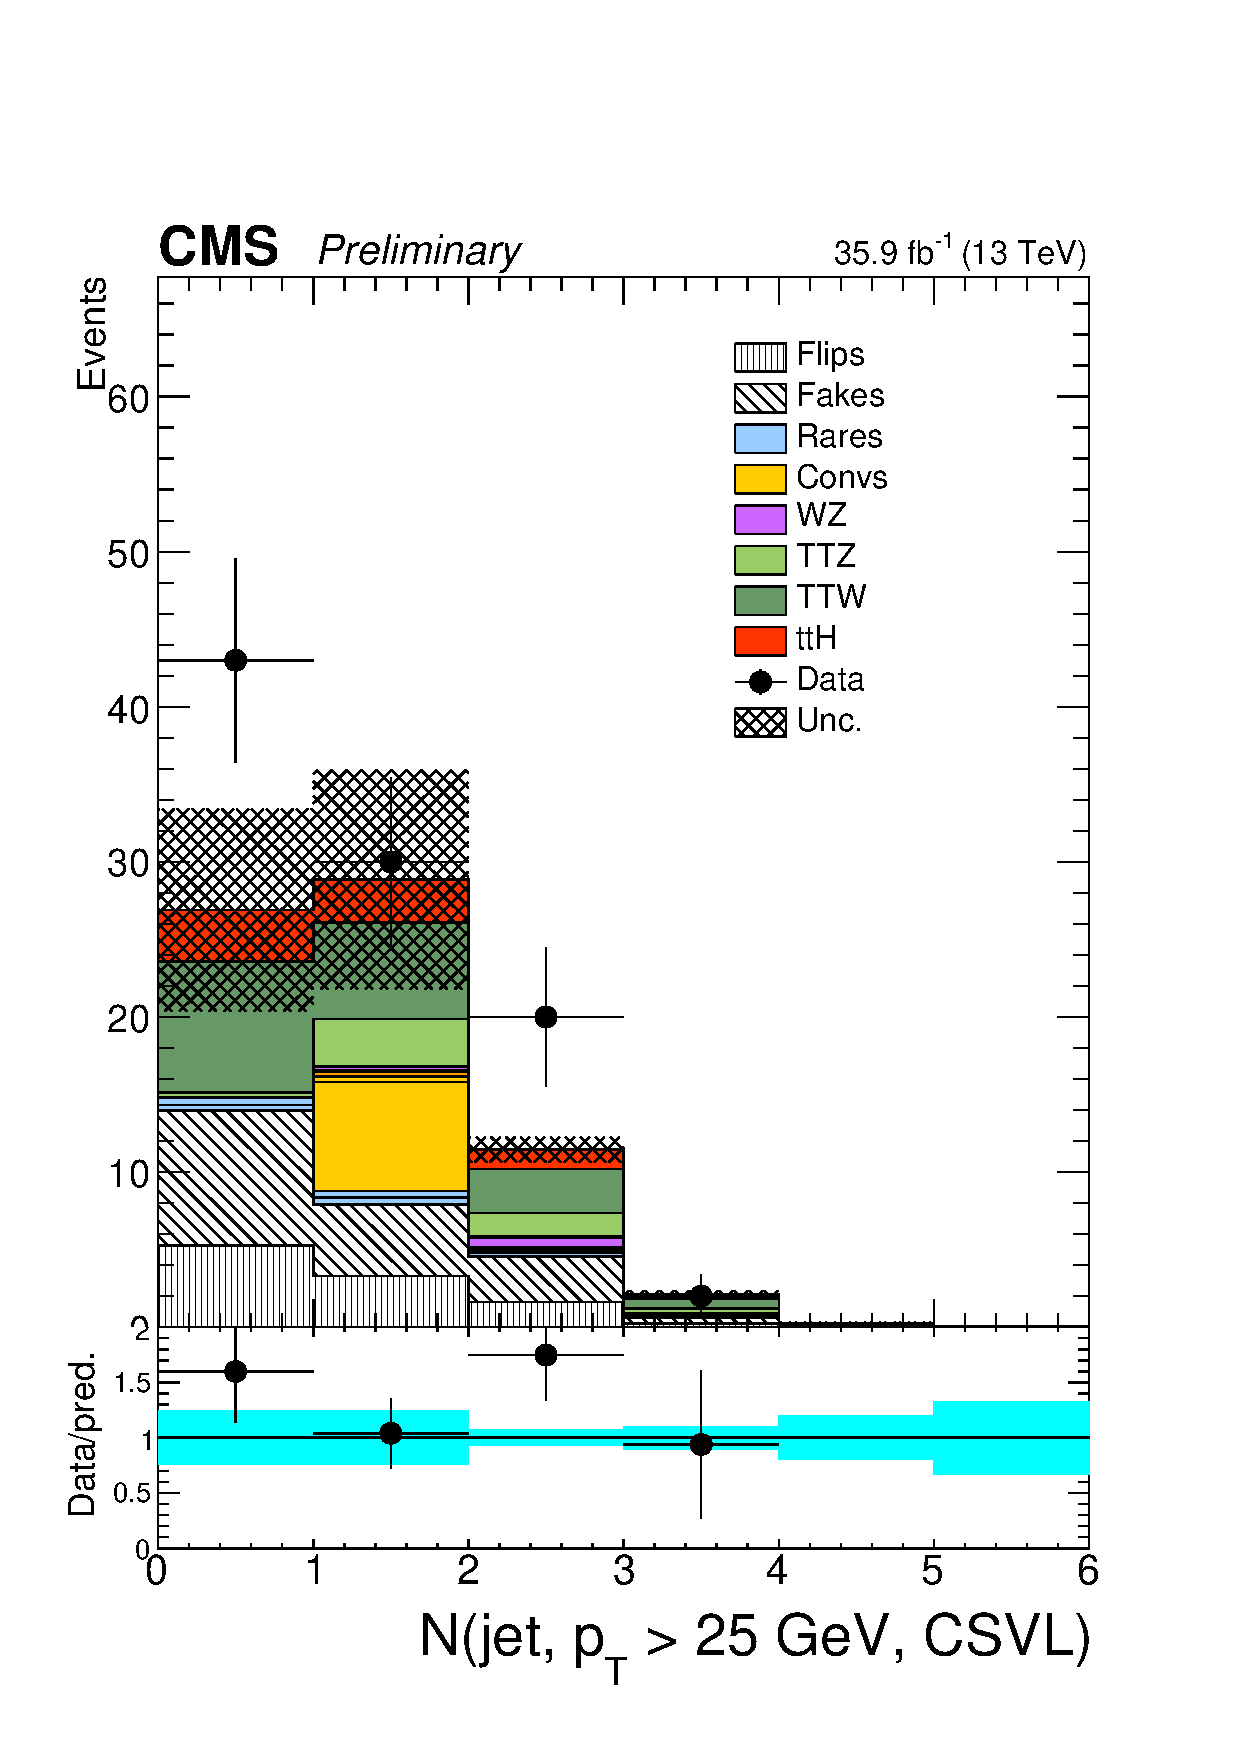
\includegraphics[width=0.32\textwidth]{ch5_figs/nJets_CSVL_ttH_ee_stackPlot_SR.pdf}
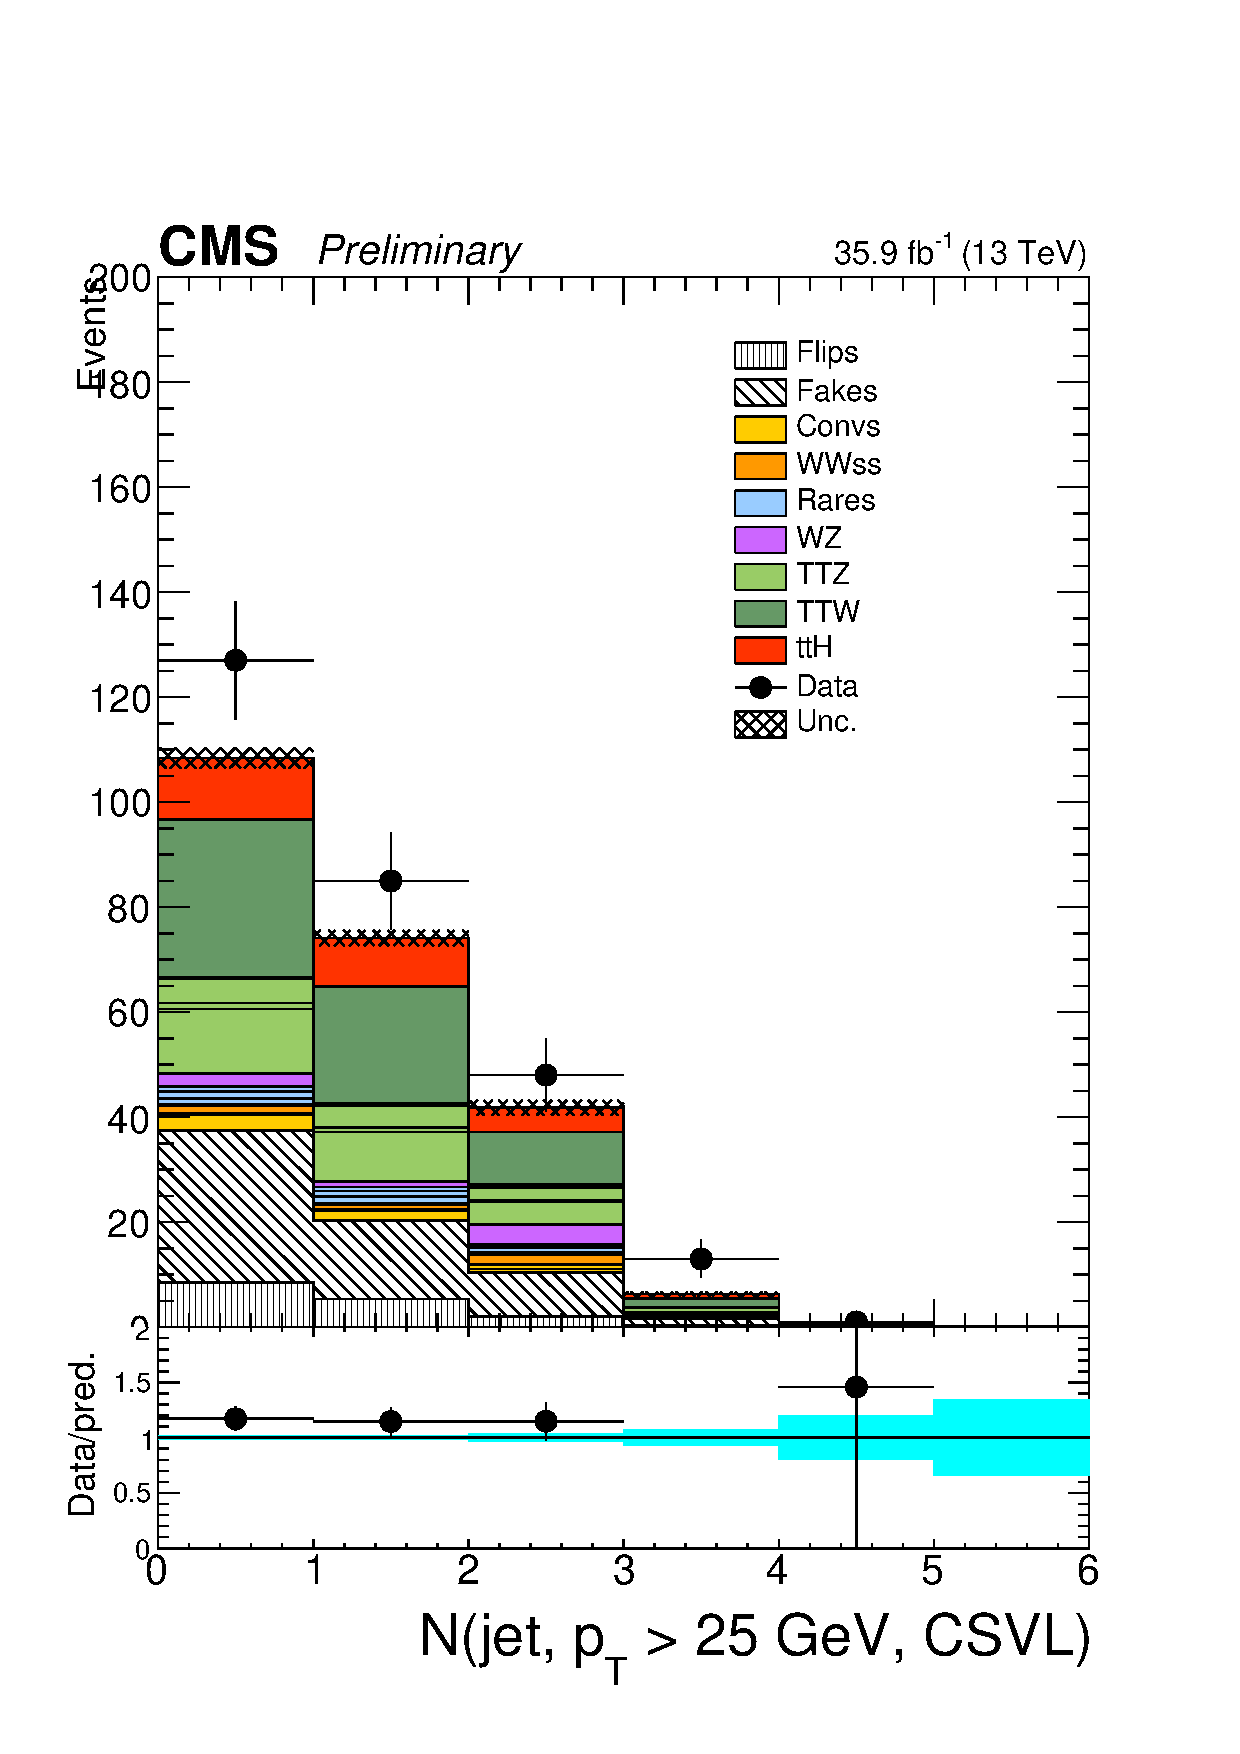
\includegraphics[width=0.32\textwidth]{ch5_figs/nJets_CSVL_ttH_em_stackPlot_SR.pdf}
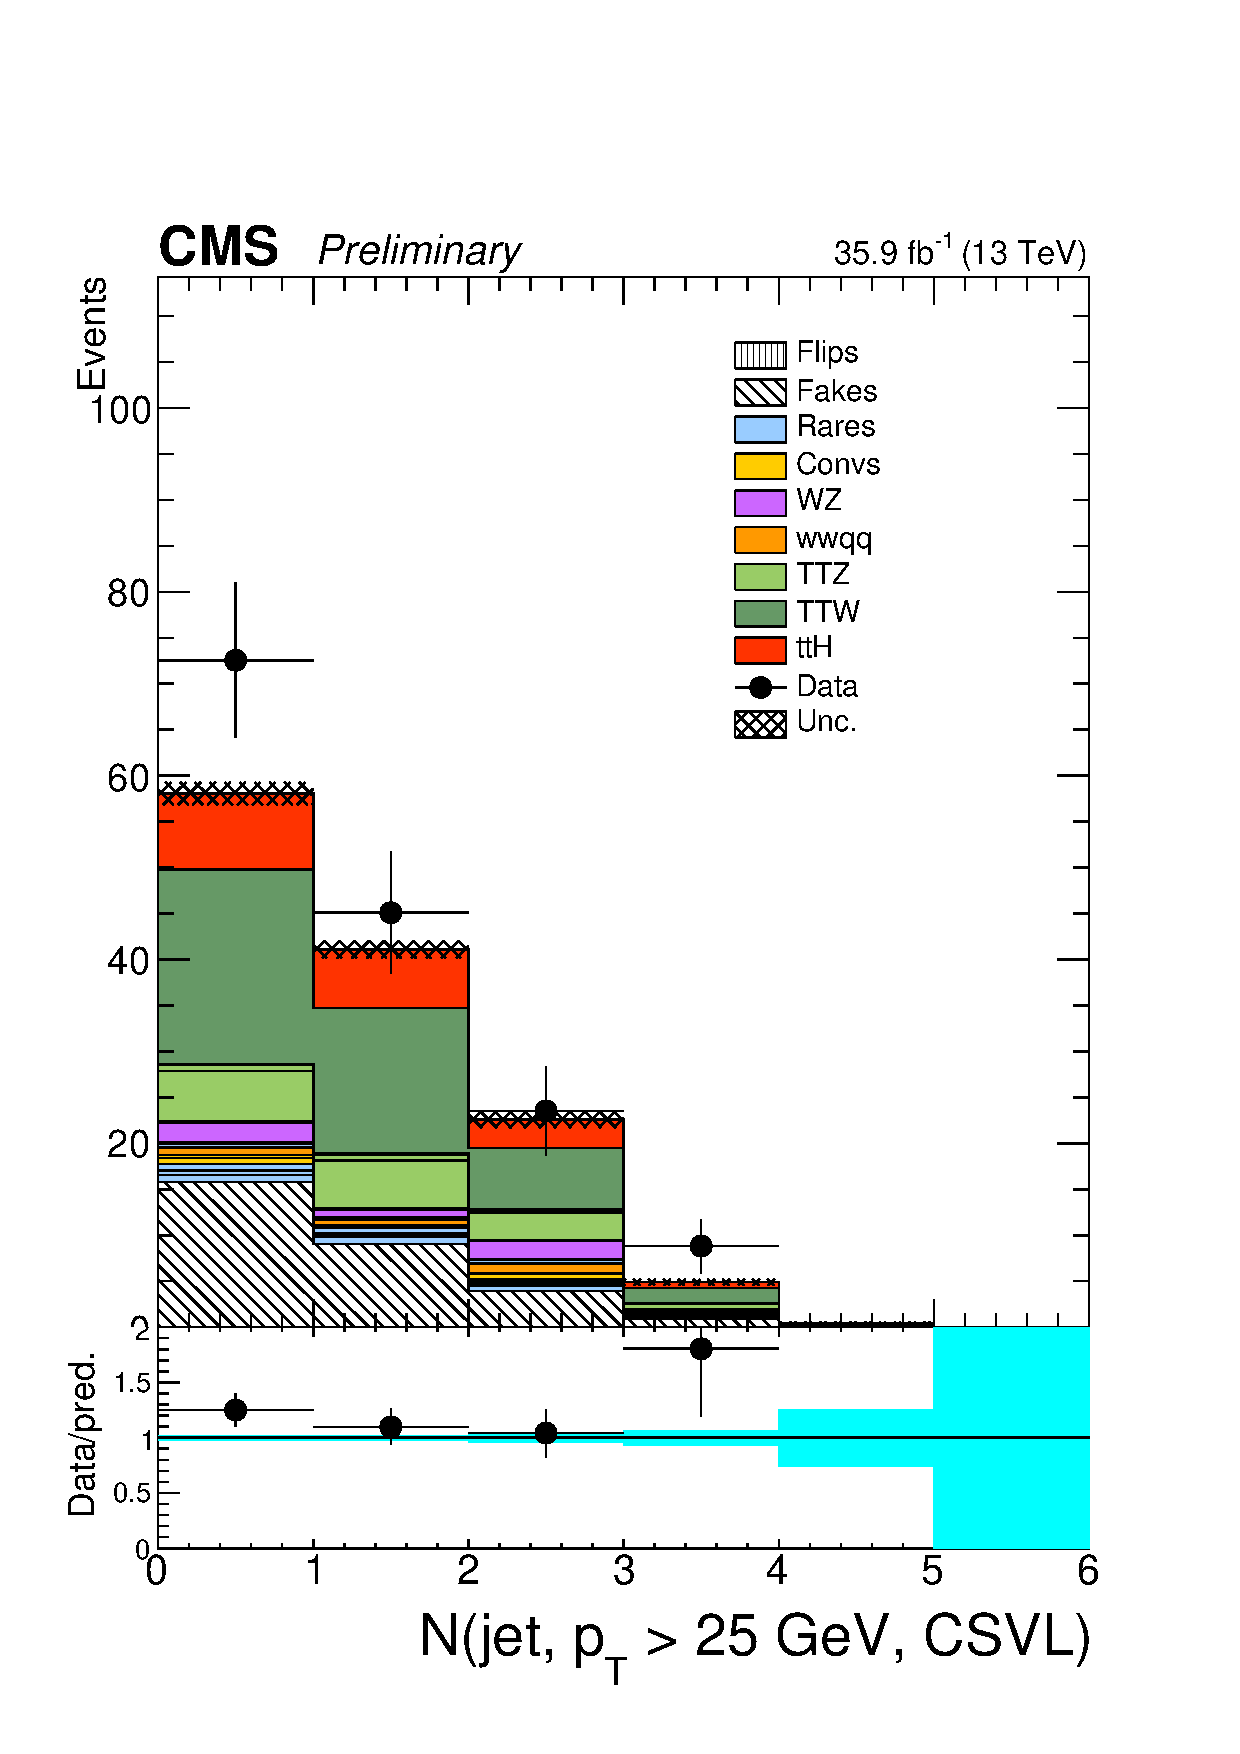
\includegraphics[width=0.32\textwidth]{ch5_figs/nJets_CSVL_ttH_mm_stackPlot_SR.pdf} \\
\caption[Data/MC comparison of the CSVL jet multiplicity in the signal region]{The jet multiplicity for jets passing the loose working point of the CSV tagger in the 2lss $ee$/$e\mu$/$\mu\mu$ categories. Uncertainties shown are purely statistical.}
\label{fig:sr_njets_csvl}
\end{figure}

\begin{figure}[htp]
\centering
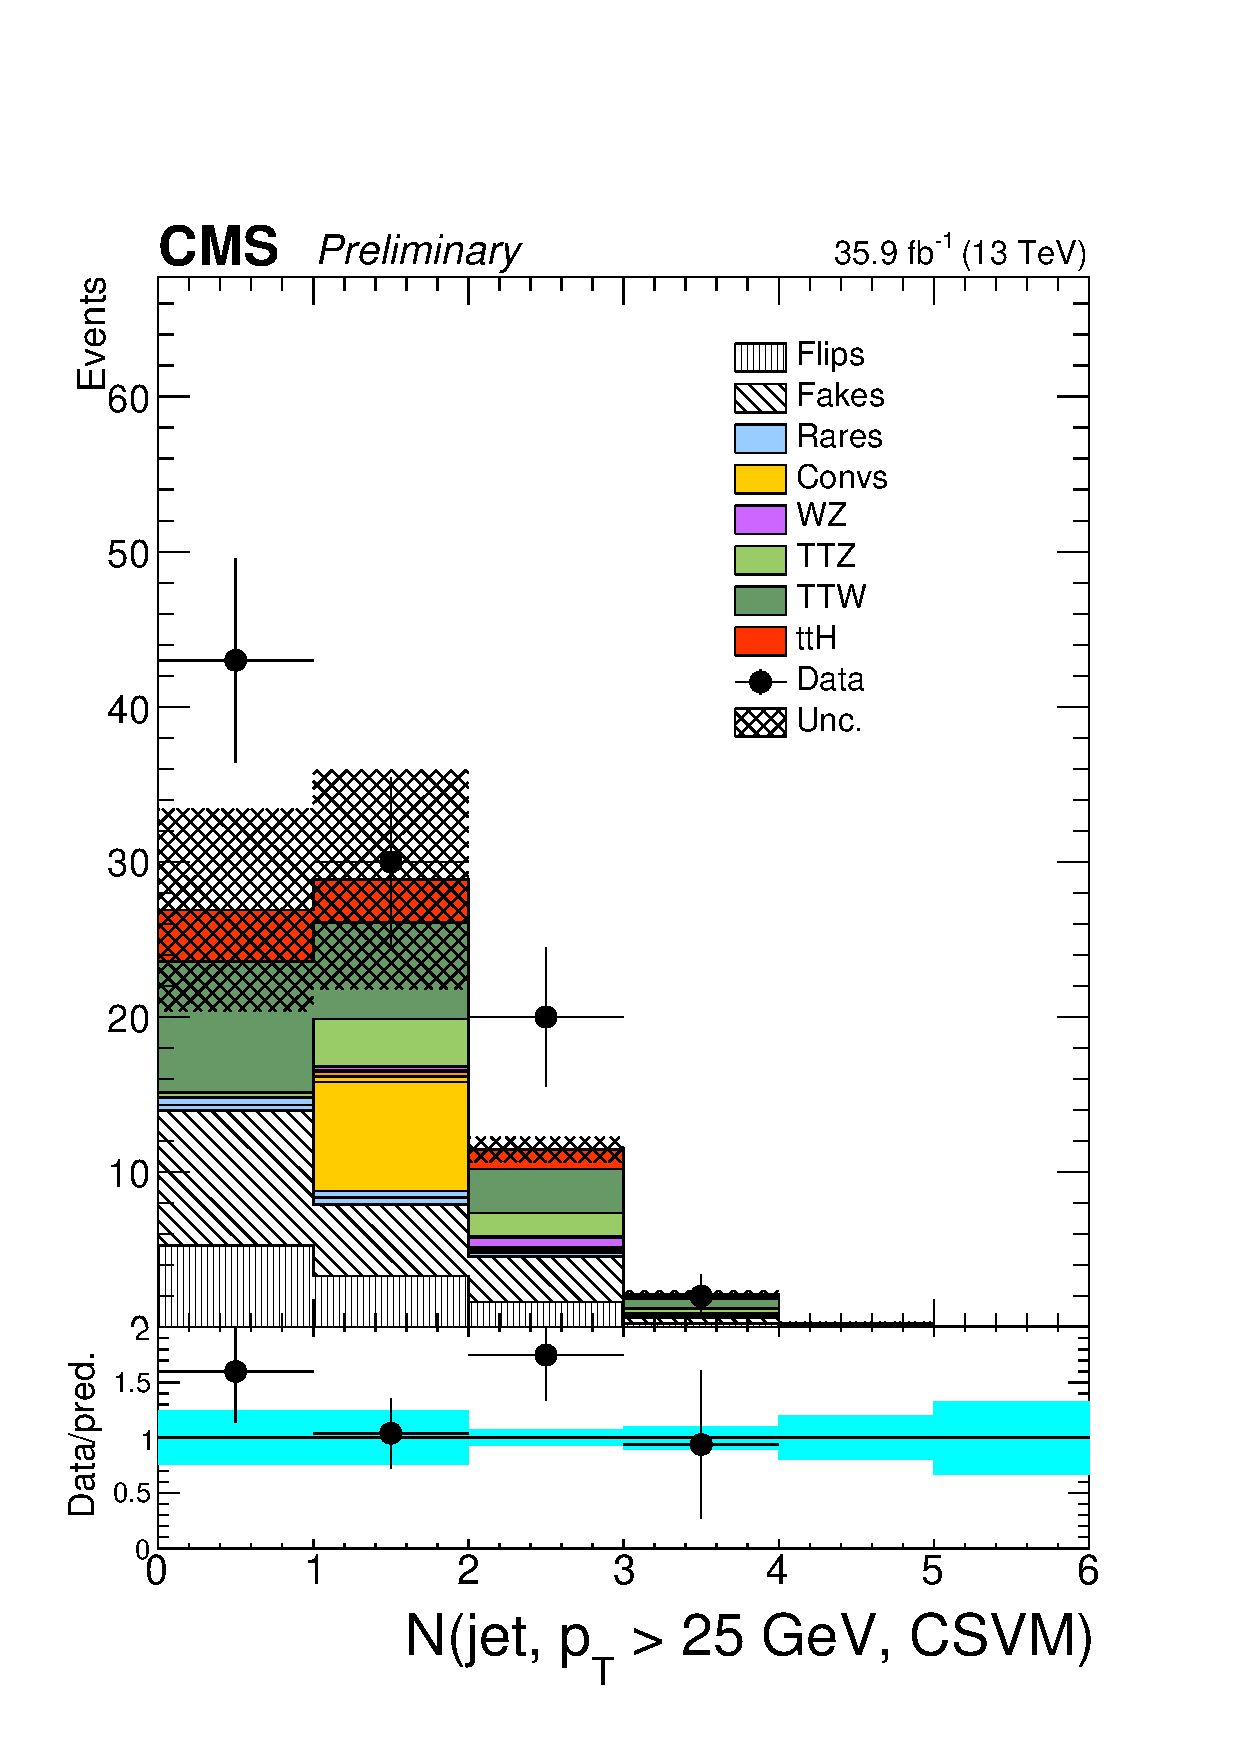
\includegraphics[width=0.32\textwidth]{ch5_figs/nJets_CSVM_ttH_ee_stackPlot_SR.pdf}
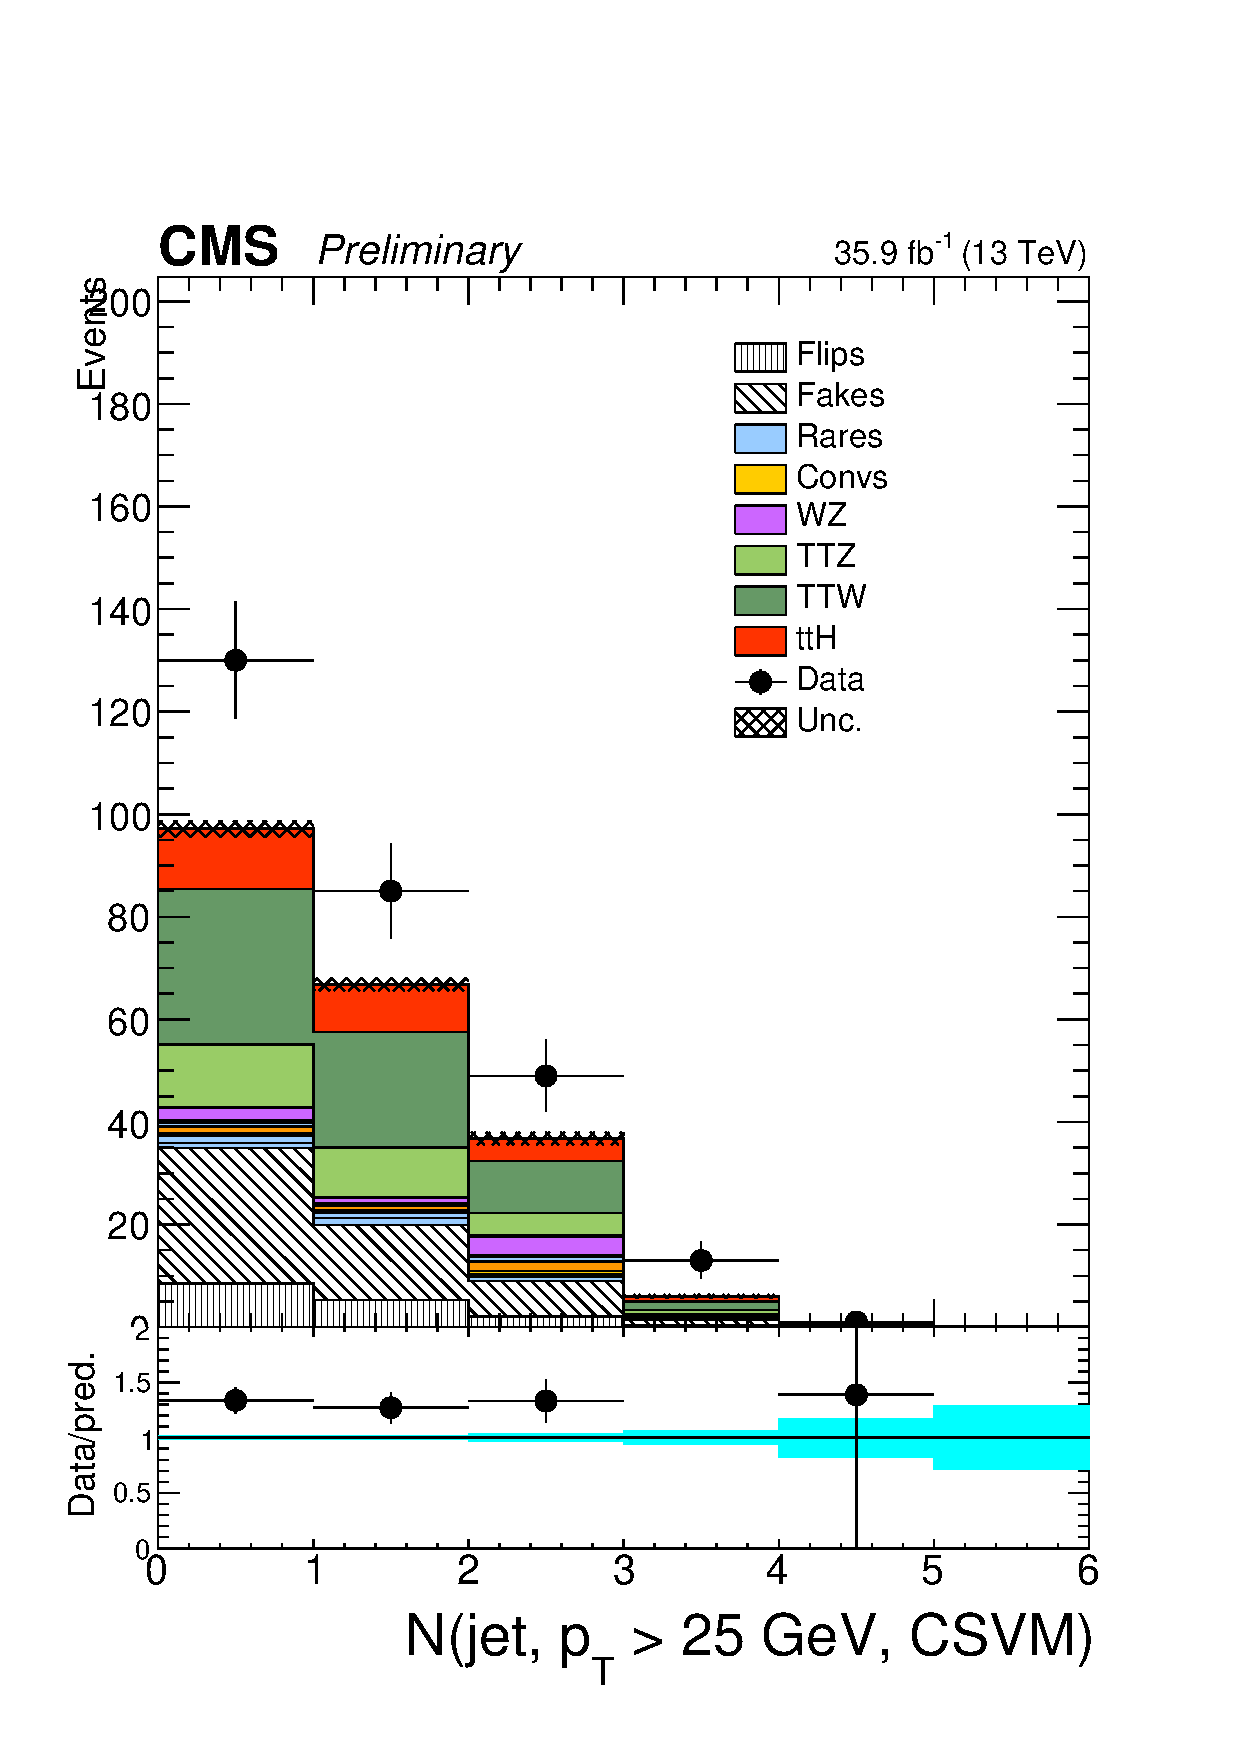
\includegraphics[width=0.32\textwidth]{ch5_figs/nJets_CSVM_ttH_em_stackPlot_SR.pdf}
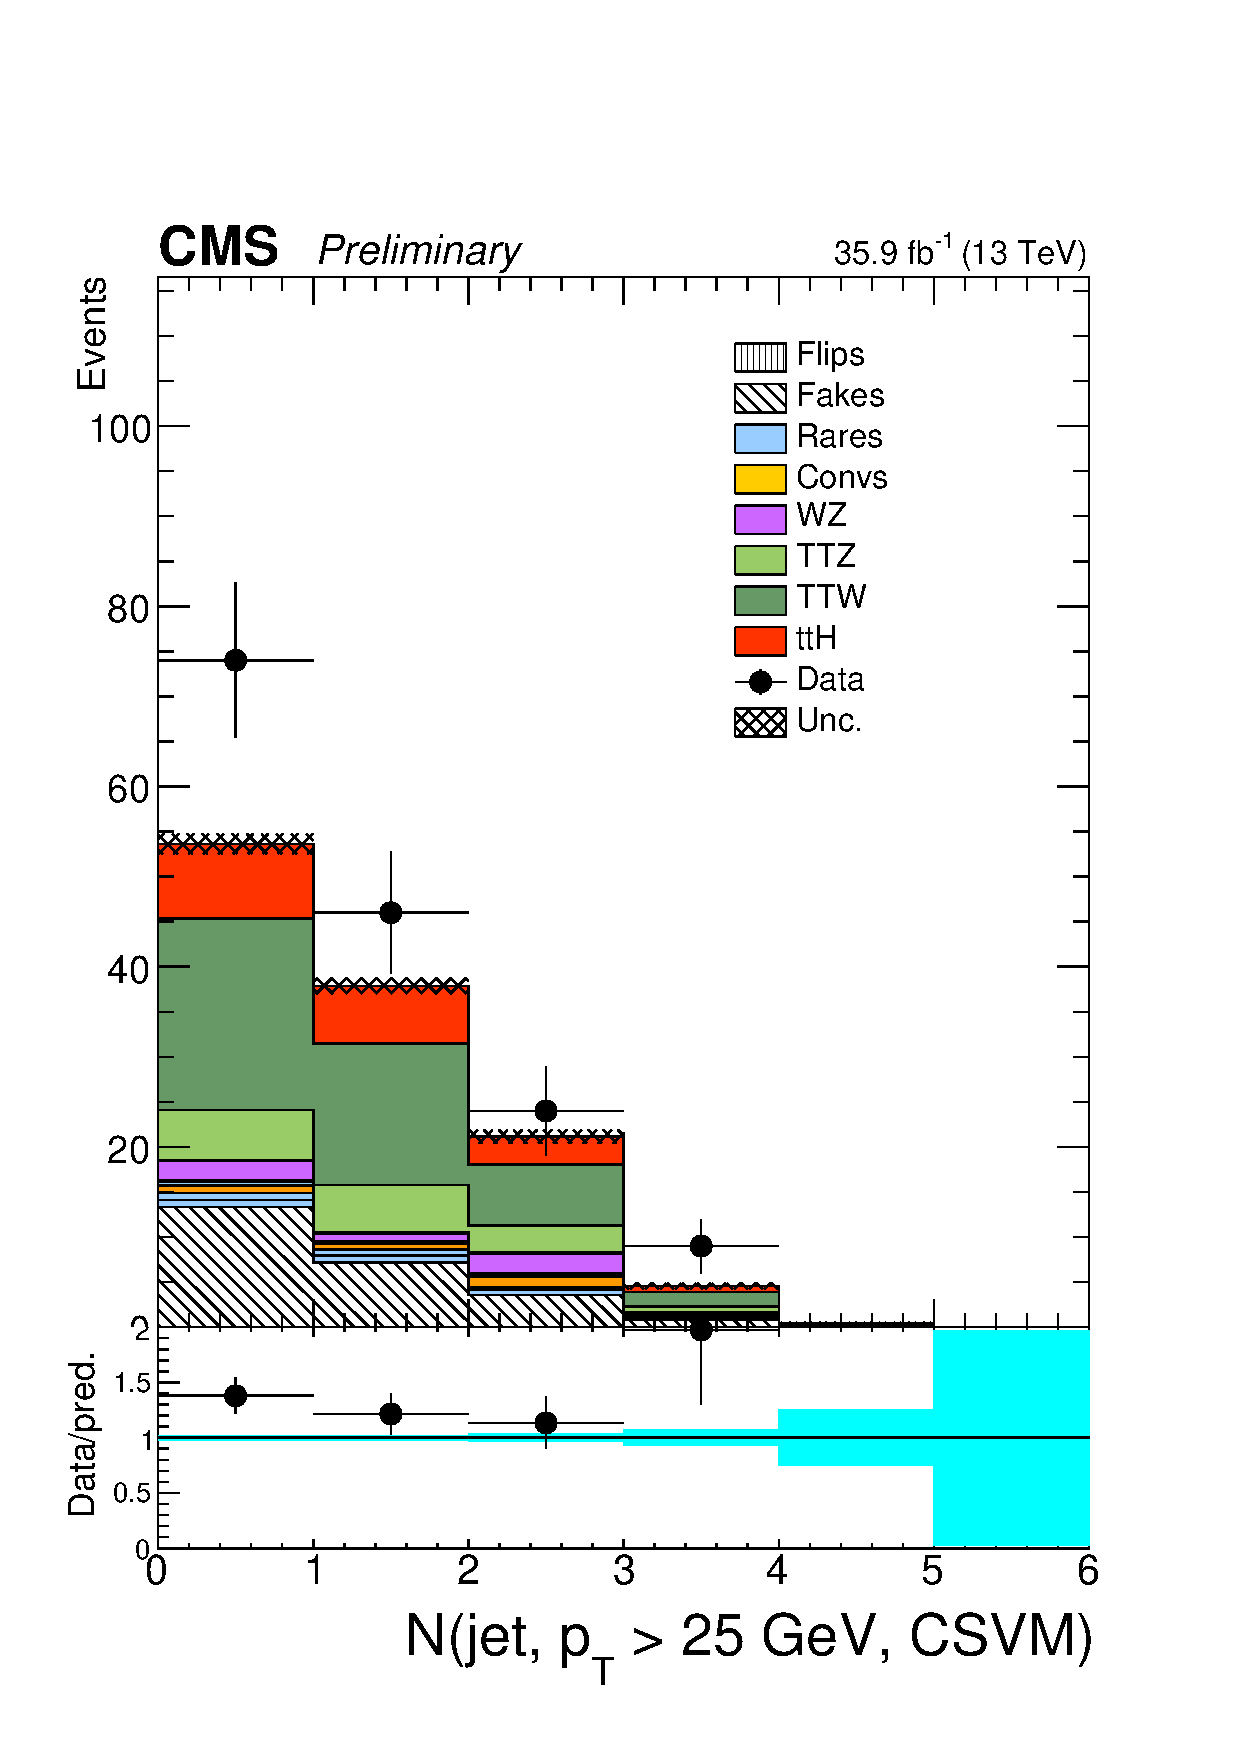
\includegraphics[width=0.32\textwidth]{ch5_figs/nJets_CSVM_ttH_mm_stackPlot_SR.pdf} \\
\caption[Data/MC comparison of the CSVM jet multiplicity in the signal region]{The jet multiplicity for jets passing the medium working point of the CSV tagger in the 2lss $ee$/$e\mu$/$\mu\mu$ categories. Uncertainties shown are purely statistical.}
\label{fig:sr_njets_csvm}
\end{figure}

\begin{figure}[htp]
\centering
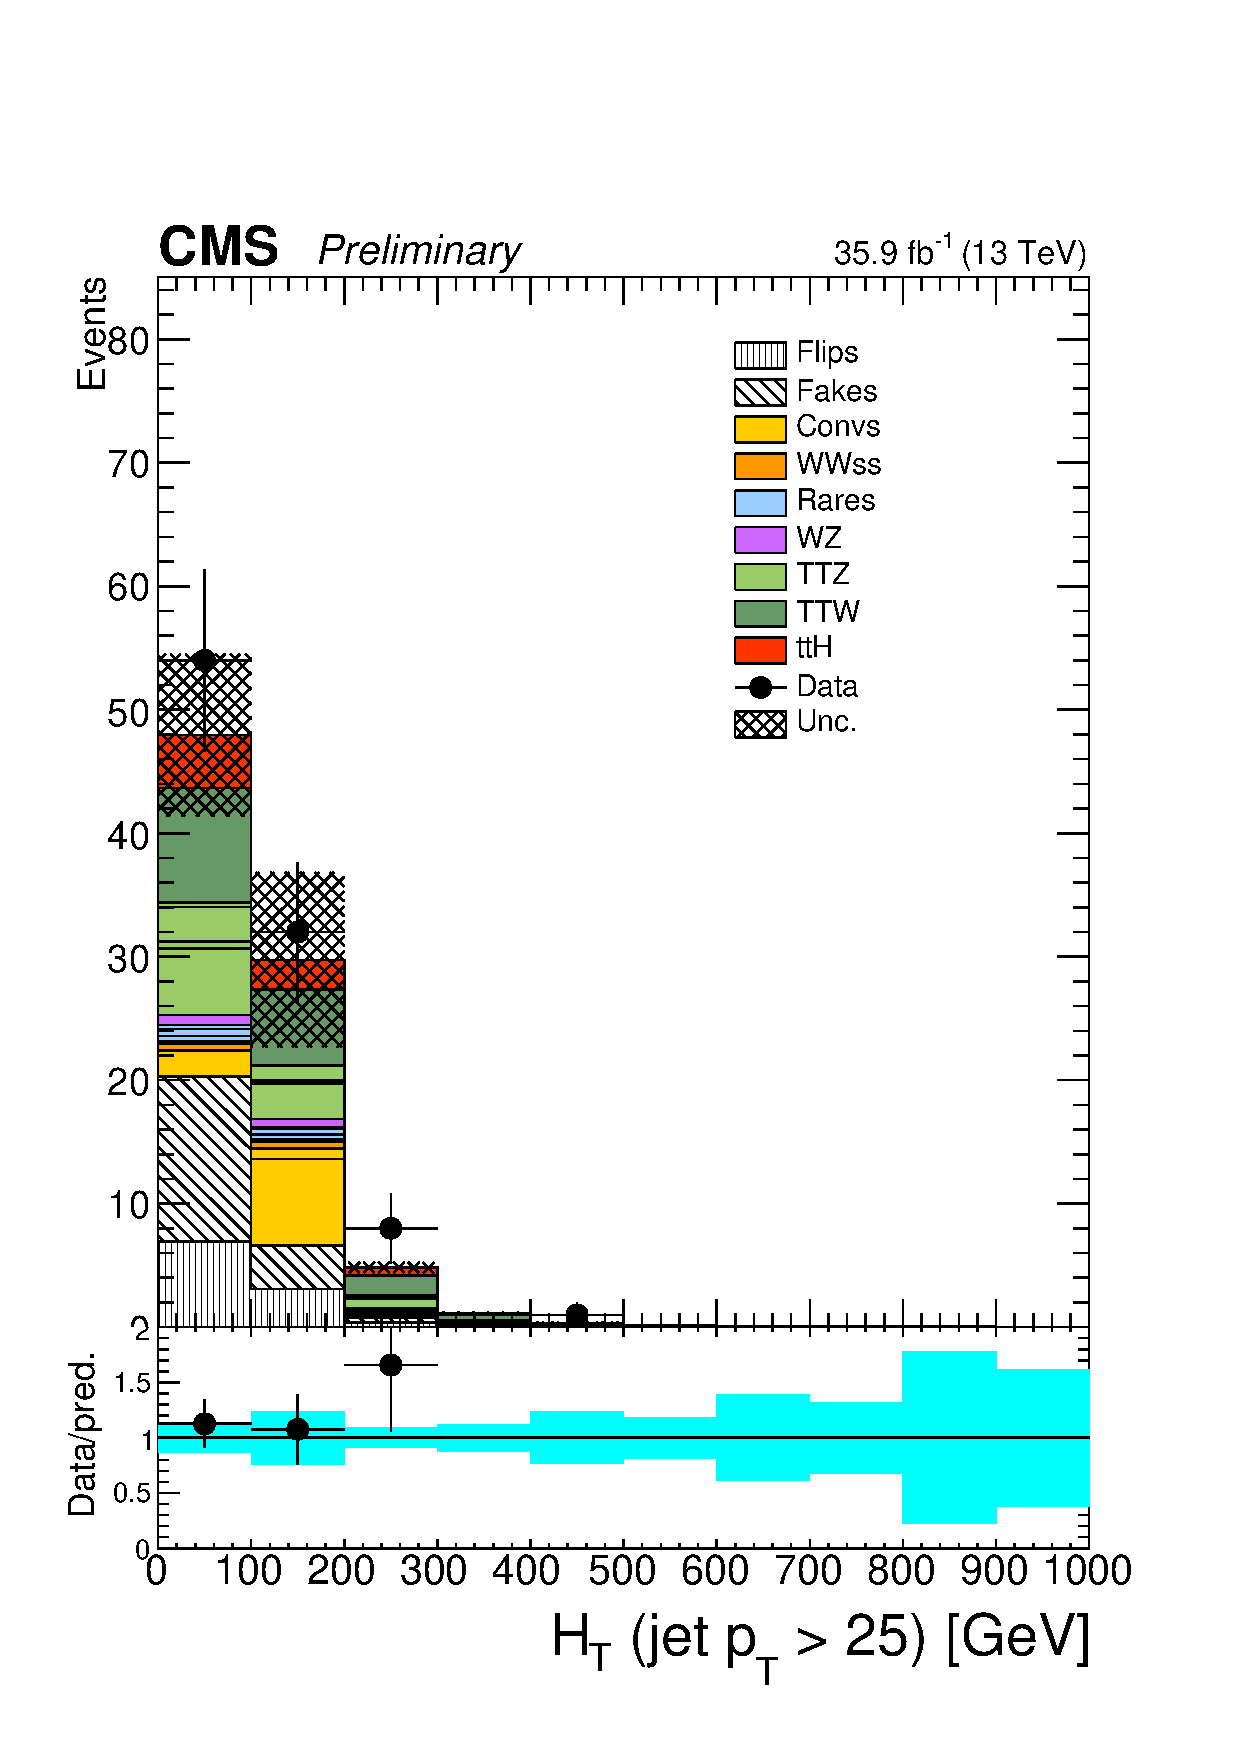
\includegraphics[width=0.32\textwidth]{ch5_figs/ht_ttH_ee_stackPlot_SR.pdf}
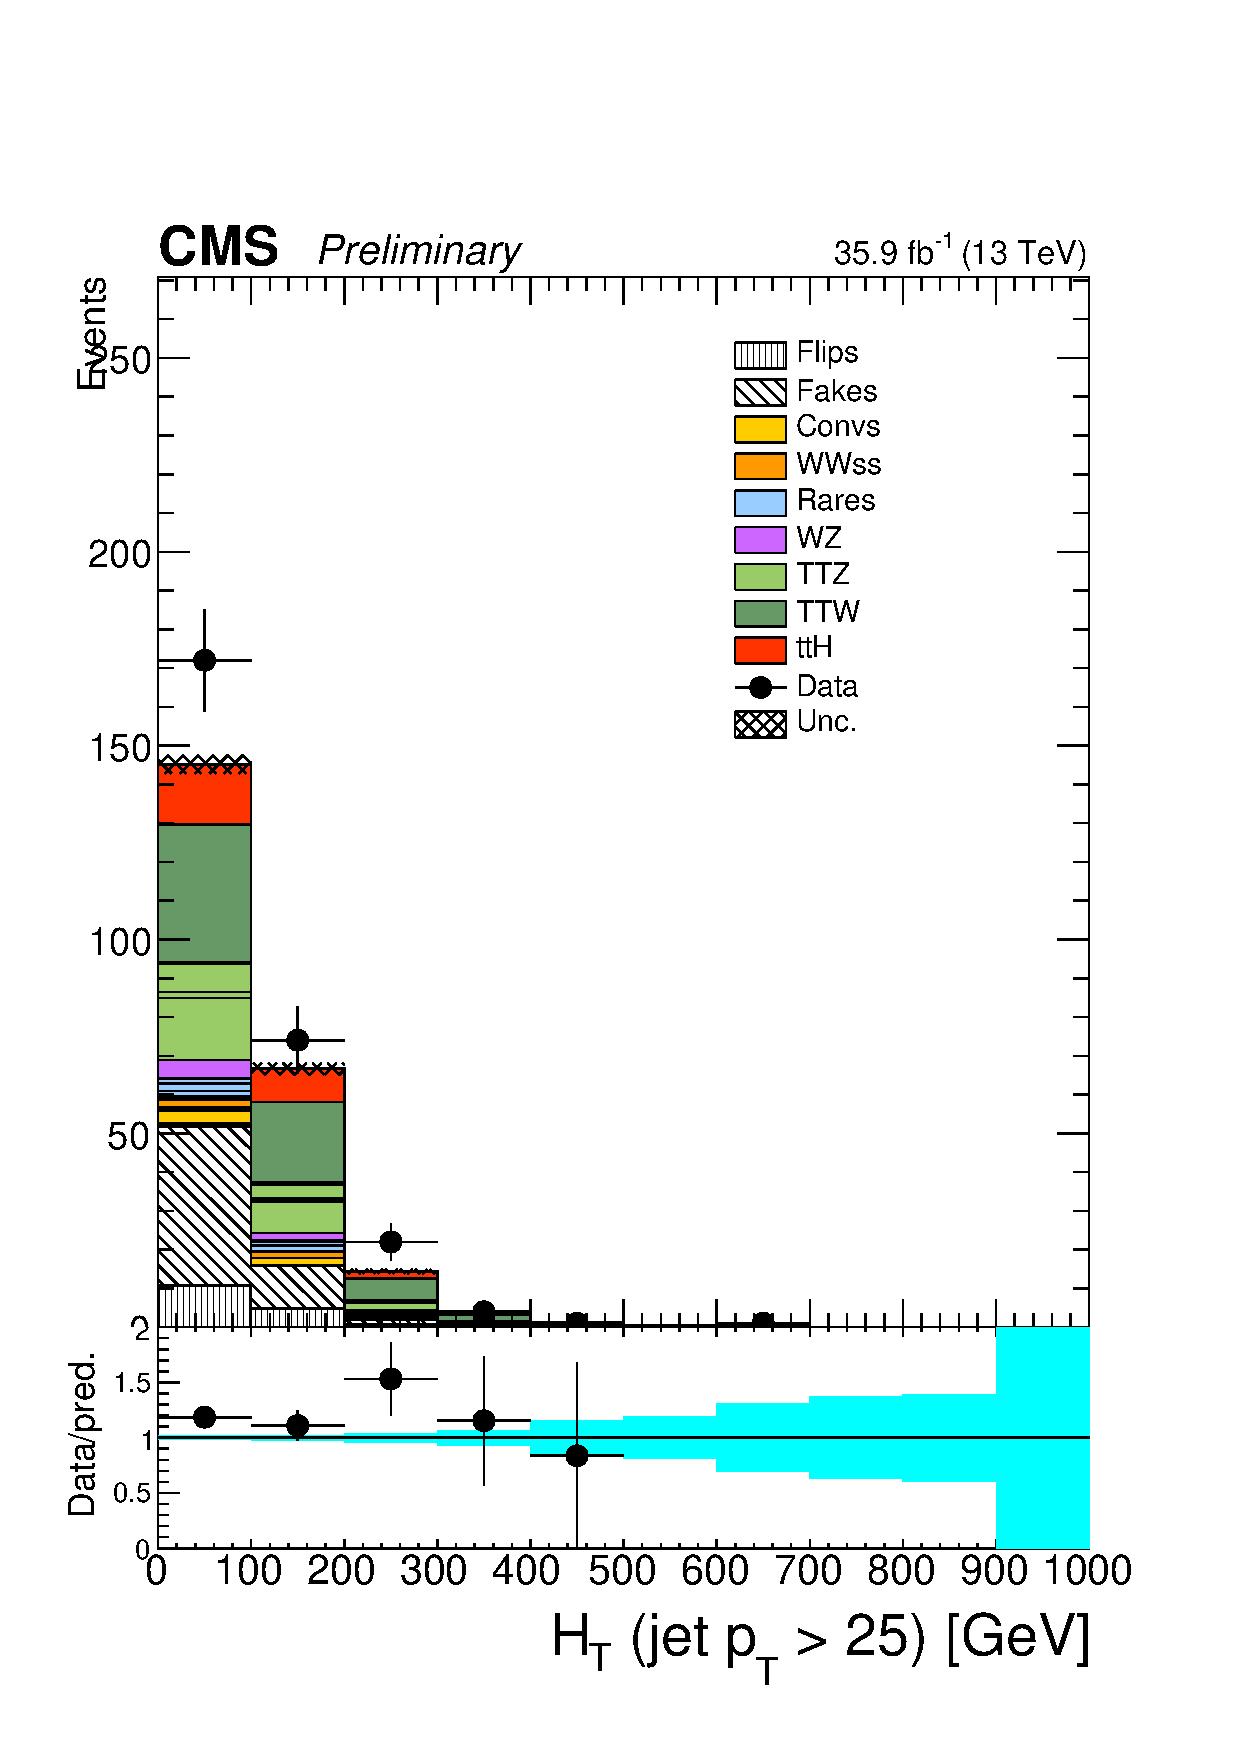
\includegraphics[width=0.32\textwidth]{ch5_figs/ht_ttH_em_stackPlot_SR.pdf}
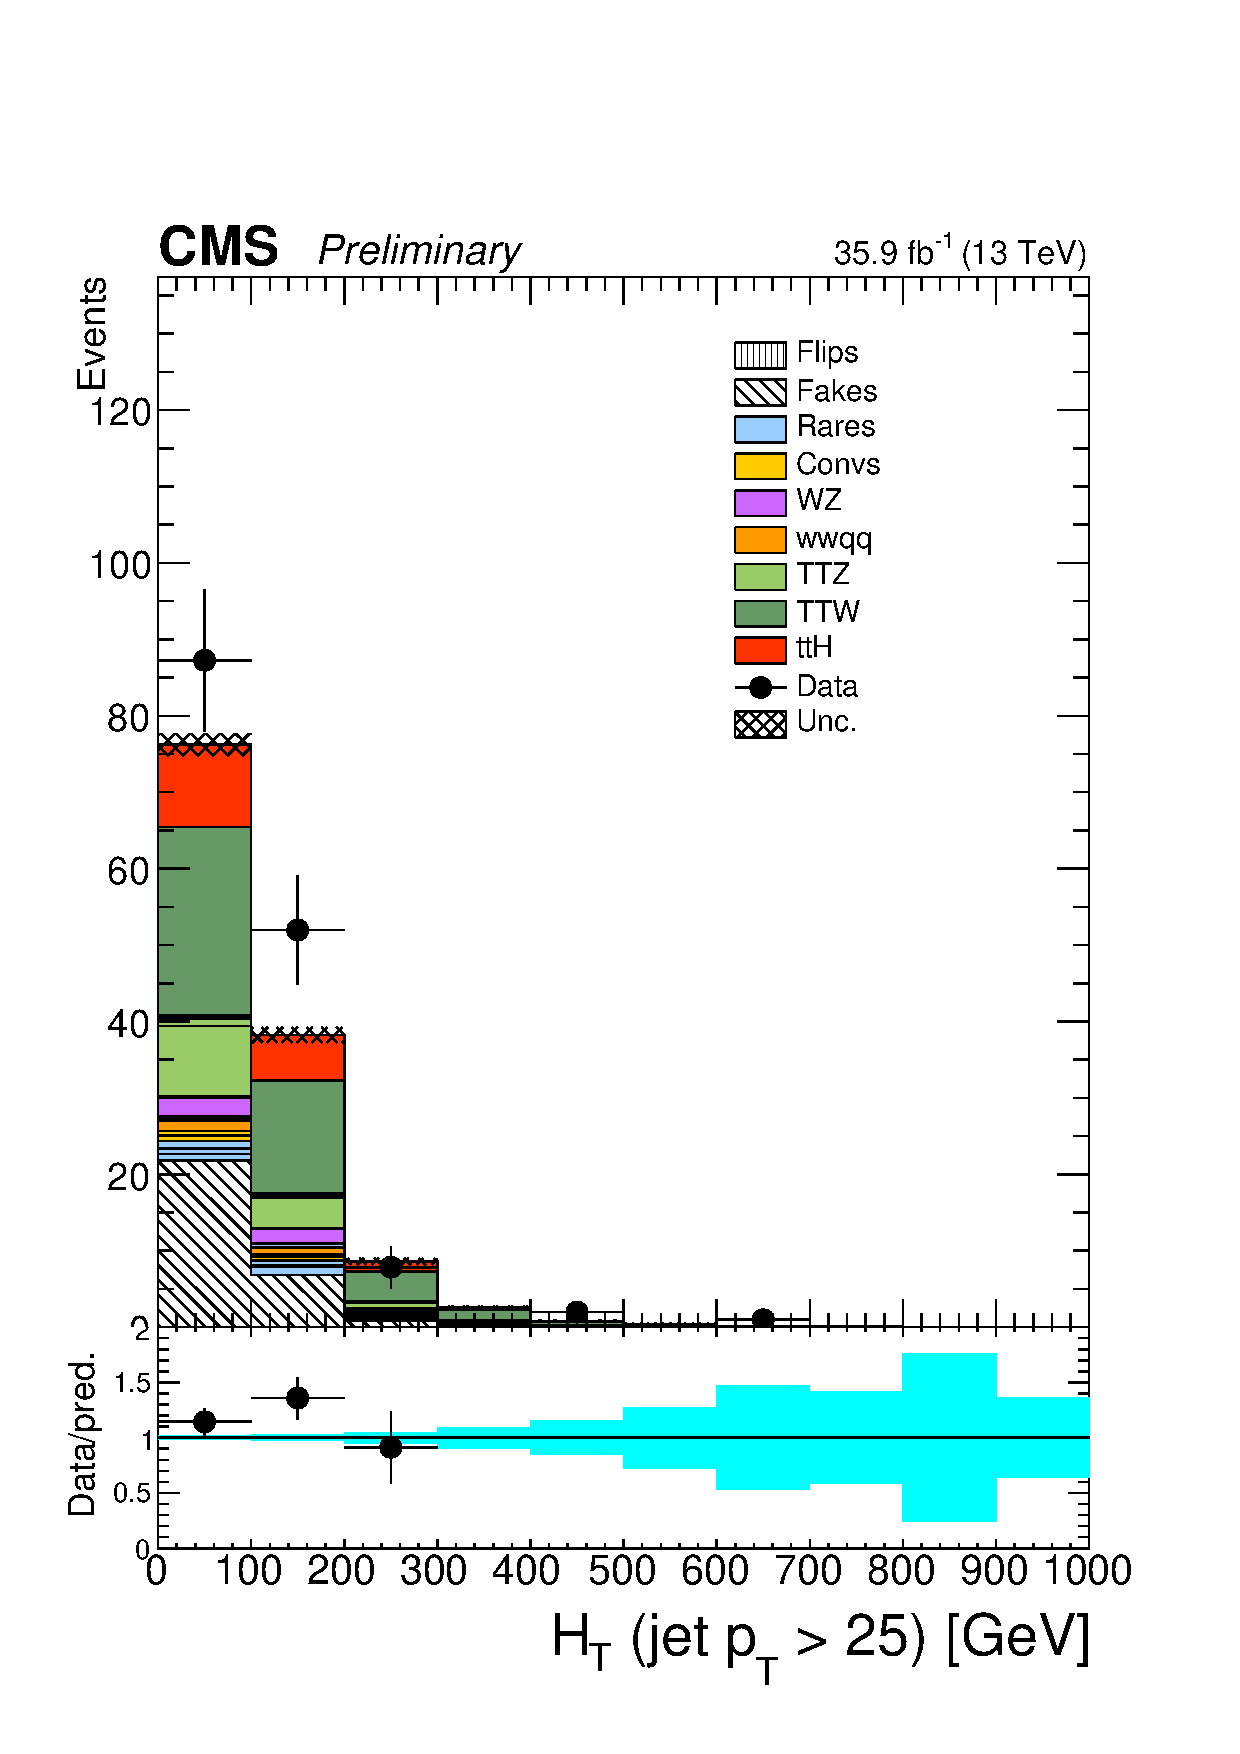
\includegraphics[width=0.32\textwidth]{ch5_figs/ht_ttH_mm_stackPlot_SR.pdf} \\
\caption[Data/MC comparison of the \ht spectra in the signal region]{The \ht spectra in the 2lss $ee$/$e\mu$/$\mu\mu$ categories. Uncertainties shown are purely statistical.}
\label{fig:sr_ht}
\end{figure}

\begin{figure}[htp]
\centering
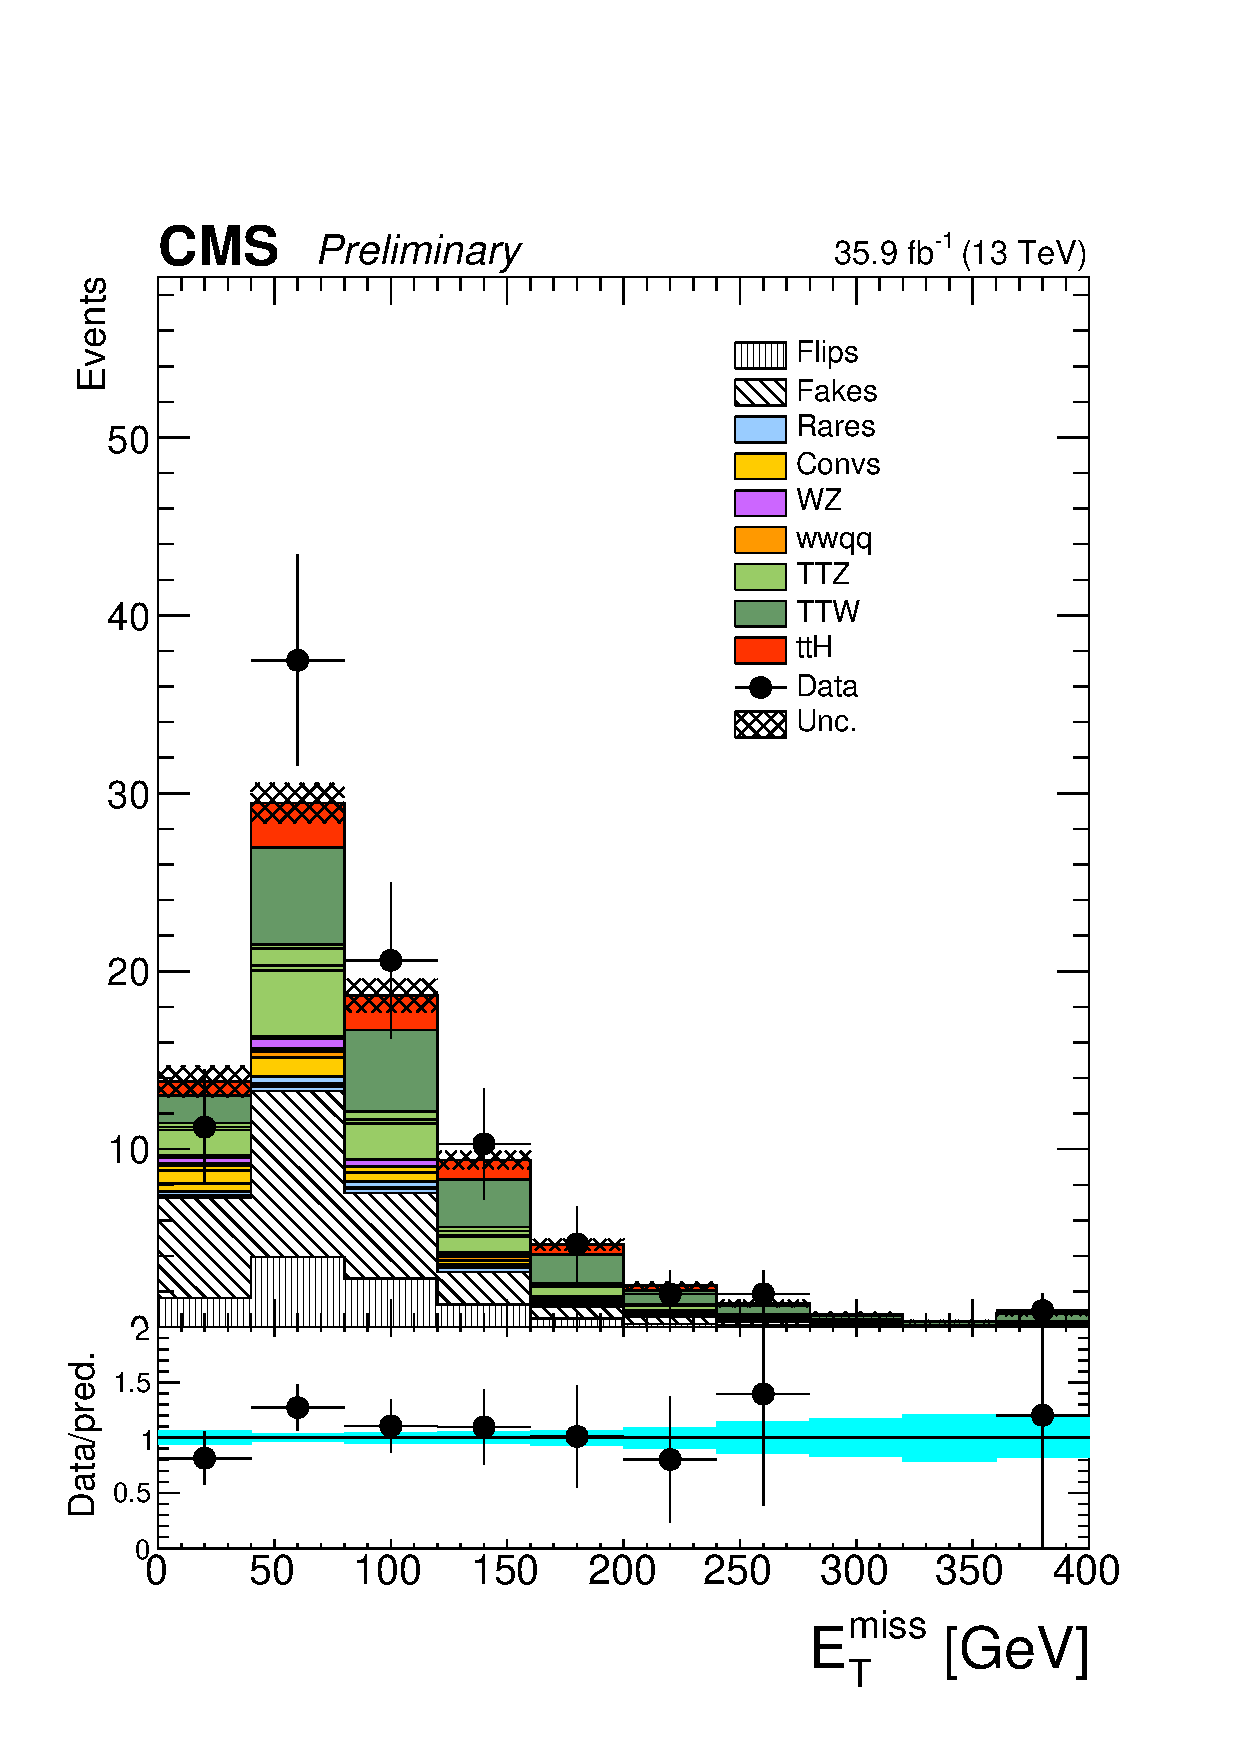
\includegraphics[width=0.32\textwidth]{ch5_figs/met_ttH_ee_stackPlot_SR.pdf}
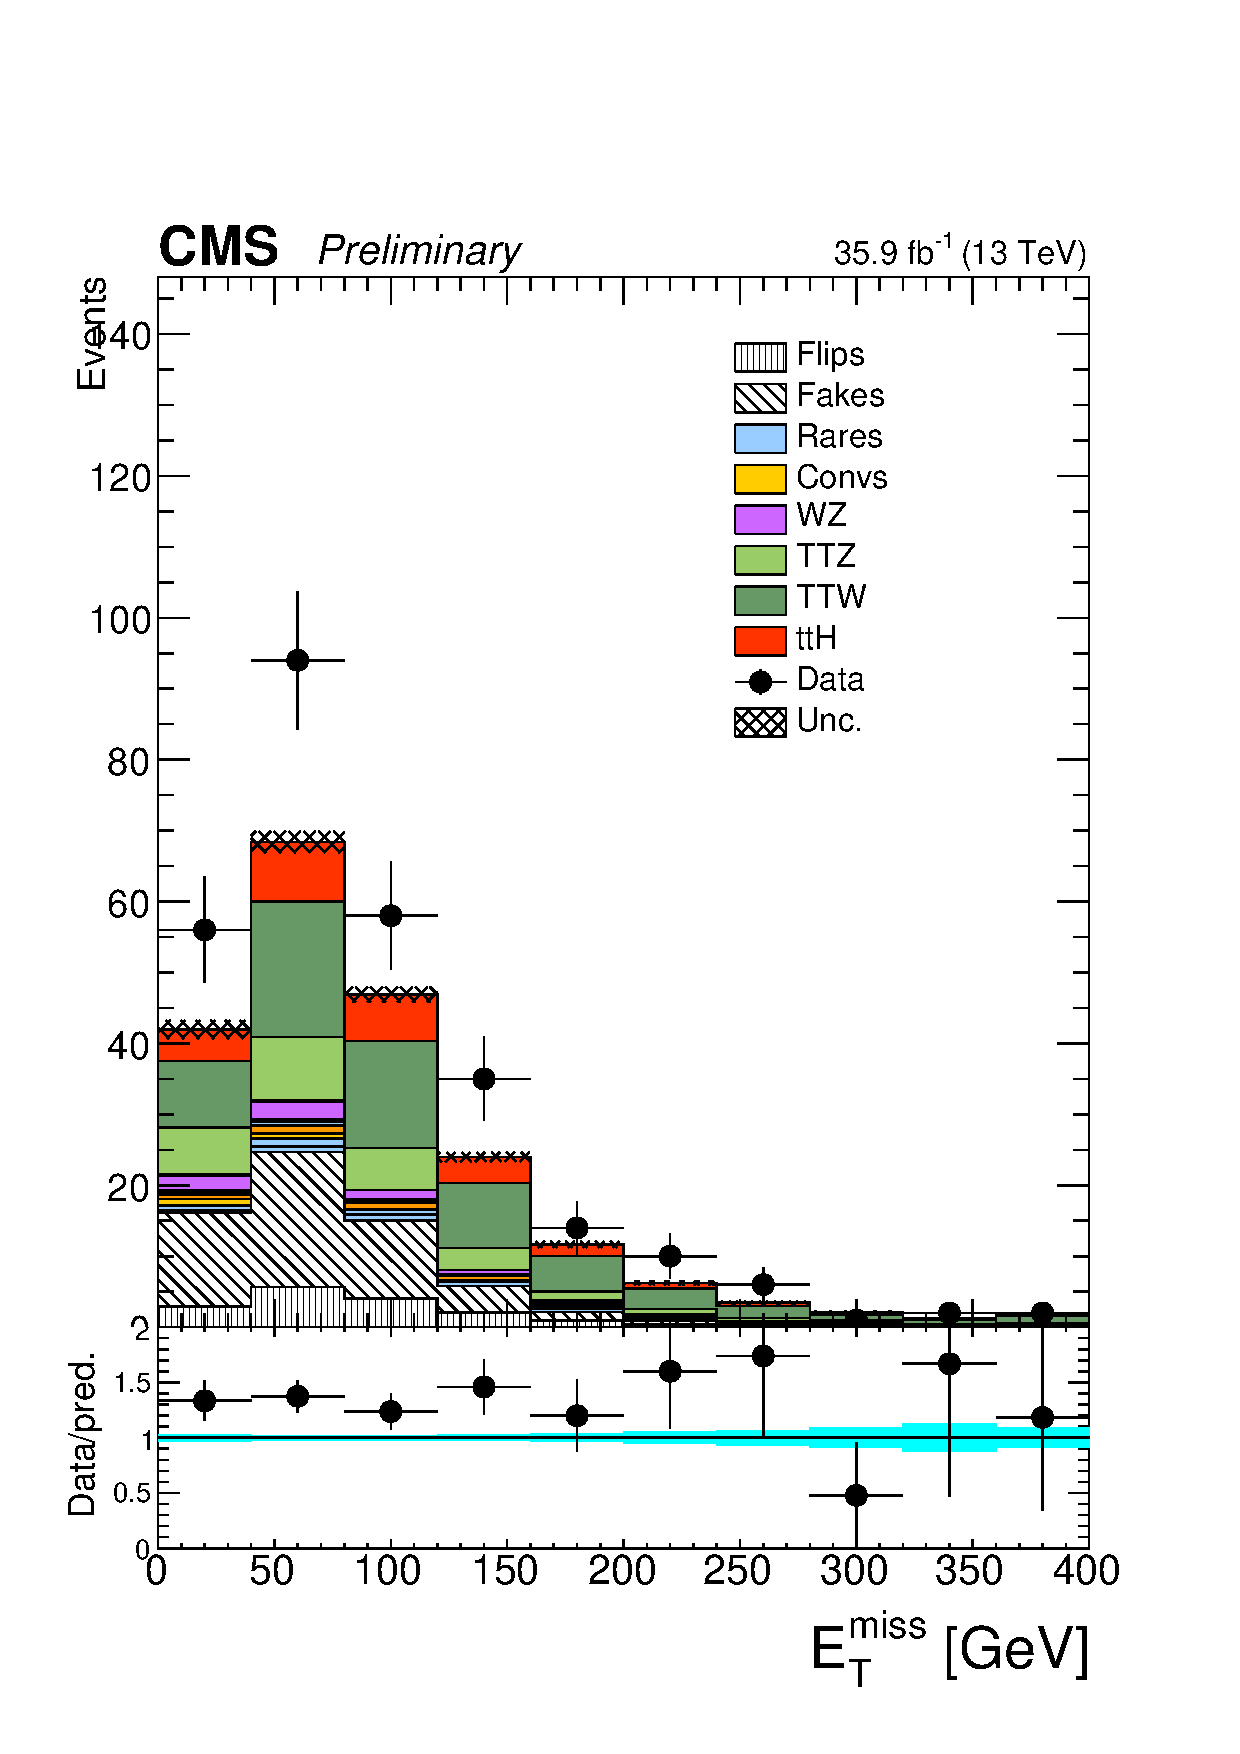
\includegraphics[width=0.32\textwidth]{ch5_figs/met_ttH_em_stackPlot_SR.pdf}
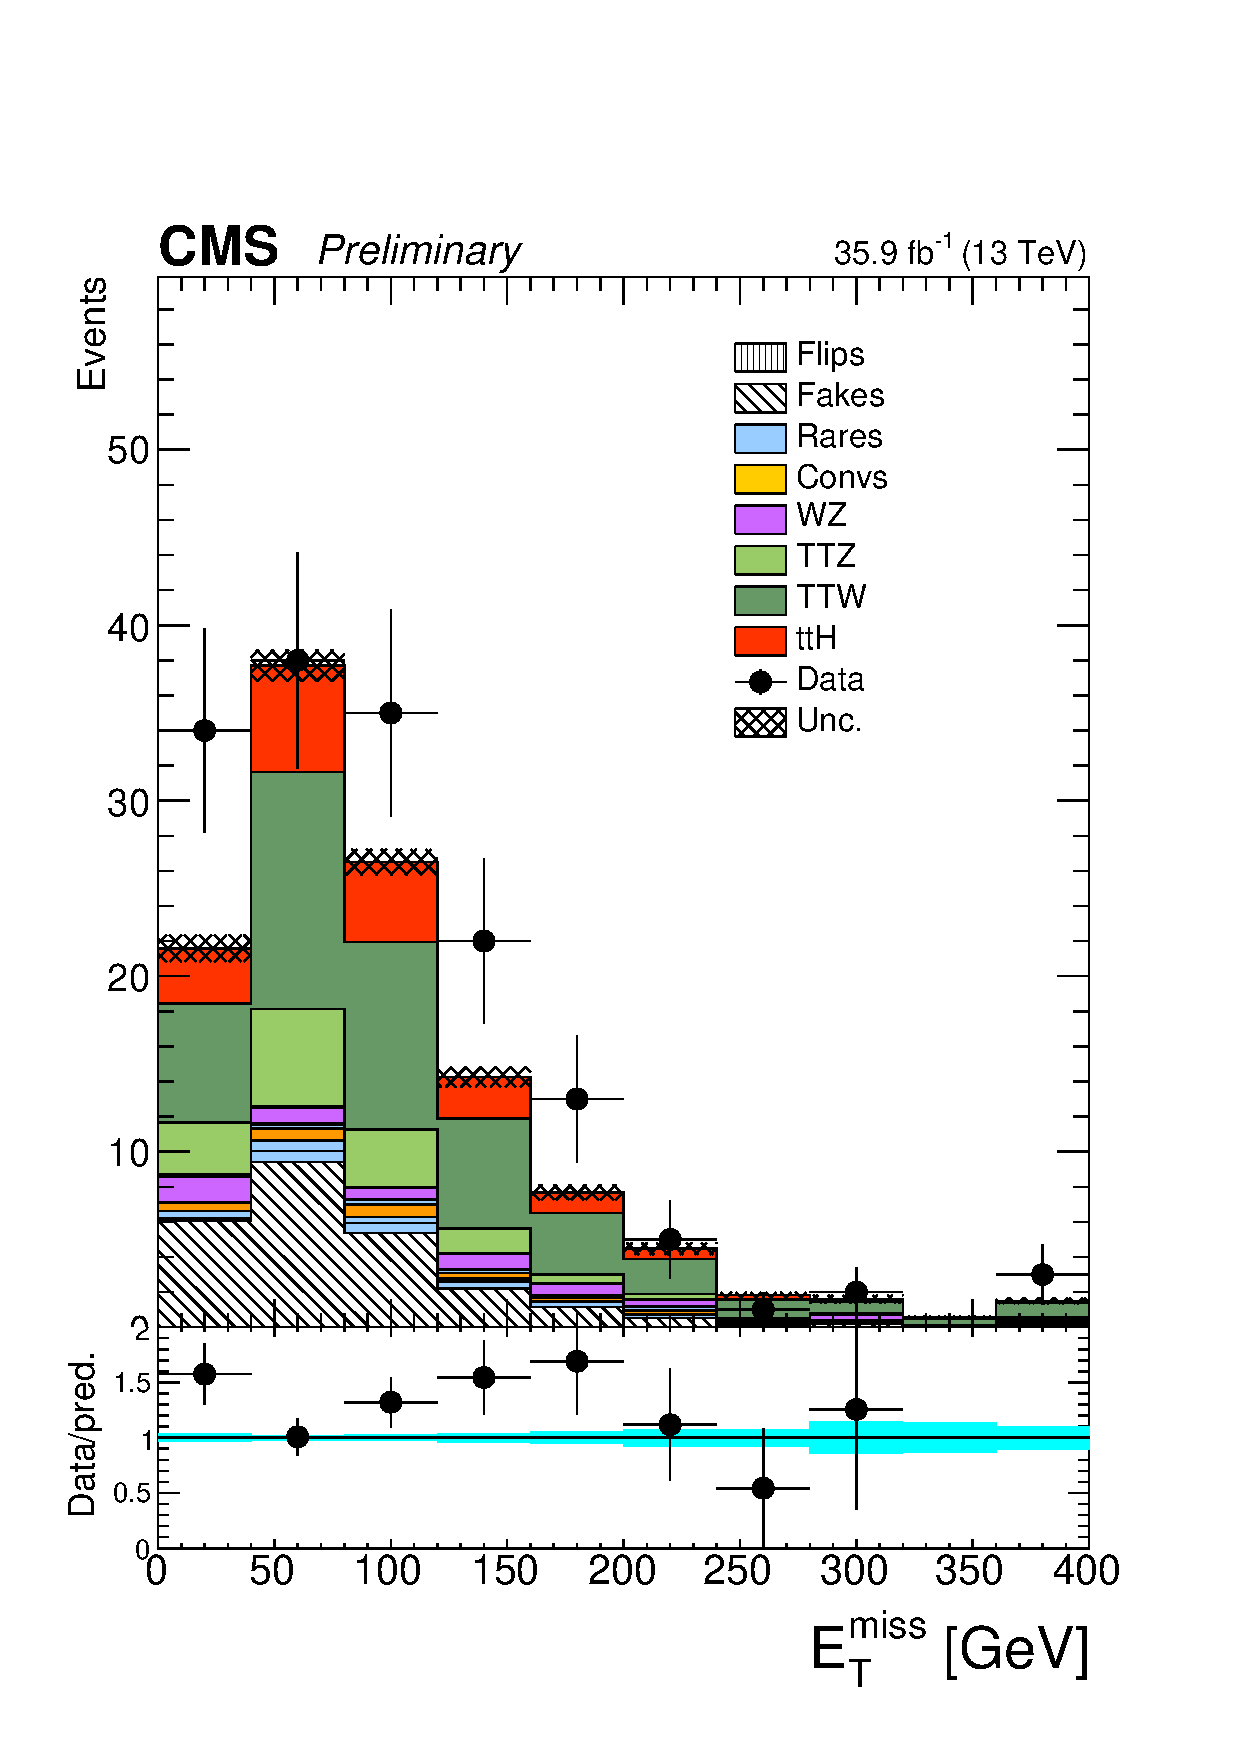
\includegraphics[width=0.32\textwidth]{ch5_figs/met_ttH_mm_stackPlot_SR.pdf} \\
\caption[Data/MC comparison of the \met in the signal region]{The \met spectra in the 2lss $ee$/$e\mu$/$\mu\mu$ categories. Uncertainties shown are purely statistical.}
\label{fig:sr_met}
\end{figure}

\begin{figure}[htp]
\centering
\includegraphics[width=0.32\textwidth]{ch5_figs/metLD_ttH_ee_stackPlot_SR.pdf}
\includegraphics[width=0.32\textwidth]{ch5_figs/metLD_ttH_em_stackPlot_SR.pdf}
\includegraphics[width=0.32\textwidth]{ch5_figs/metLD_ttH_mm_stackPlot_SR.pdf} \\
\caption[Data/MC comparison of the \met LD distribution in the signal region]{The \met LD spectra in the 2lss $ee$/$e\mu$/$\mu\mu$ categories. Uncertainties shown are purely statistical.}
\label{fig:sr_metLD}
\end{figure}

%
% Chapter 6
%

\chapter{DATA AND MC SAMPLES}
\section{Data samples}
\section{Signal MC samples}
\section{Background MC samples}
\section{Triggers}
%% \begin{figure}[hbtp]
%%  \begin{center}
%%    \includegraphics[width=0.8\textwidth]{ch4_figs/cms_particleflow.pdf}
%%    \caption{An overview of how CMS detects different types of particles. The slice of CMS in in the x-y plane.~\cite{NEED CITATION}.}
%%    \label{fig:cms_pflow}
%%  \end{center}
%% \end{figure}

%
% Chapter 7
%

\chapter{BACKGROUND PREDICTIONS}
\label{chap:background}
Despite optimizing the event selection criteria to select signal events, a substantial amount of background from a variety of processes enters the signal region.
These backrounds are classified as being either reducible or irreducible, and are estimated differently depending on this classification. An understanding
of each background process and a proper assessment of the uncertainity associated with the estimation of each background is critical to extracting the signal and interpreting
the results. 

\section{Reducible backgrounds}
Reducible backgrounds arise from a number of sources, but always contain leptons that are either non-prompt, or have a lepton whose electric charge is mismeasured.
These backgrounds are classified as reducible because if the event selection and CMS object reconstruction worked with perfect efficiency, the events would not
enter the signal region; thus, improving the prompt lepton identifiction and CMS lepton electric charge measurement can reduce the contributions from these processes.
Reducible backgrounds are estimated via data-driven approaches using control regions and extrapolation techniques to predict their contribution to the yield in the
signal region. The background due to fakes is entirely separate from the charge mismeasurement background and are estimated separately. 

\subsection{Fake lepton background} 
The fake lepton background gets its name from the fact that events with non-prompt leptons pass the tight selection and enter the signal region by faking prompt leptons. These
fakes typically originate from leptonic decays of certain hadrons, such as the B, D, $\Lambda$, and K. The primary source is the relatively large cross-section semi-leptonic \ttbar
process, where the b-jet from the leptonic top quark produces a fake lepton that passes the tight lepton selection criteria, but also includes other processes where a lepton
is produced inside a jet. The background from these events is estimated via a loose-to-tight extrapolation. This begins with measuring the rate at which the leptons passing
the fakeable selection also pass the tight selection, known as the fake rate. The measurement is performed in a control region of the data, known as the measurement region (see below).
The measurement is then used to extrapolate from a sideband with fakeable leptons to estimate the contribution in the signal region 
from events with fake leptons. 

The measurement region is heavily enriched in QCD multijet events, which provide a
source of mostly fake leptons. The fake rate is defined as the probability of a non-prompt lepton which passes the fakeable selection to also pass the tight selection.
The measurement region events satisfy the following requirements:

\begin{itemize}
 \item exactly one fakeable lepton
 \item one preselected jet with $\Deta$R $>$ 0.7 from the lepton
 \item $M_{T}(l,\met) < 15$ GeV
\end{itemize}

\noindent This selection enriches the measurement region with non-prompt leptons. The data analyzed in the measurement region is collected on single lepton
triggers which require a single lepton and a particle-flow jet with \pt $>$ 30 GeV.

To ensure a high purity of fake leptons in the measurement region, the contribution of prompt leptons must be accounted for. This contribution arises from W and Z plus jets processes, but also from \ttbar. The Z contamination
is addressed by vetoing events with more than one loose lepton. The prompt leptons from W decays is subtracted with a fit to the transverse mass of the lepton and missing energy, $M_{T}(l,E_{T}^{miss})$. A cut is first applied requiring
$M_{T}(l,E_{T}^{miss}) < $15 GeV, with the residual contamination subtracted in each \pt bin using W/Z +jet MC. 

The final fake rates are shown in Figure~\ref{fig:fakerate}. The larger uncertainties for higher \pt leptons is due to the larger uncertainties from the prompt lepton subtraction method. A good agreement between data and MC is observed overall.
In this analysis, electrons from photon conversions are treated as a separate background and estimated via MC. The fake rate in the measurement region for electrons is scaled by the ratio of fake rate including electrons from conversions to
the fake rate excluding electrons from conversions from QCD MC. 

\begin{figure}[htp]
\centering
\includegraphics[width=0.39\textwidth]{ch7_figs/fr_mu_barrel.pdf}
\includegraphics[width=0.39\textwidth]{ch7_figs/fr_el_barrel.pdf}\\
\includegraphics[width=0.39\textwidth]{ch7_figs/fr_mu_endcap.pdf}
\includegraphics[width=0.39\textwidth]{ch7_figs/fr_el_endcap.pdf}
\caption[Fake rate measurements in data and MC.]{The lepton fake rates as measured in data and QCD as well as \ttbar MC. Fake rates for muons are on the left while fake rates for electrons are on the right. The fake rates
measured in the barrel are on the top while the fake rates measured in the endcaps are on the bottom.}
\label{fig:fakerate}
\end{figure}

Once the fake rate is obtained from the measurement region, it is applied in a second control region, also enriched in fakes, denoted as the application region. The weighted yields in this region constitute the background due to
fake leptons in the signal region. As such, the application region is identical to the signal region, except that the requirement of the two same-sign leptons passing the tight selection is relaxed to passing the fakeable selection,
and that at least one of these leptons fails the tight selection. The fake rate weights are expressed
in terms of event yields as a function of the number of leptons failing the tight selection in a given event. The contribution of fakes in the signal region is estimated using equation~\ref{eqn:fake_rate} below:

\begin{equation}
\label{eqn:fake_rate}
  N_{pp}^{bkg} = \frac{f_{1}}{1-f_{1}}N_{pf} + \frac{f_{2}}{1-f_{2}}N_{pf} - \frac{f_{1}f_{2}}{(1-f_{1})(1-f_{2})}N_{ff}
\end{equation}

\noindent under the assumption that the contribution of prompt leptons failing the tight selection is negligible with respect to the number of non-prompt leptons failing. Here, $N_{pp}^{bkg}$ is the background contribution from fake leptons
in the signal region, $f_{1,2}$ is the fake rate for the leading, subleading lepton calculated from the measurement region, $N_{pf}$ is the number of events in the application region with 1 prompt and 1 fake lepton, and $N_{ff}$ is the
number of events in the application region with two fake leptons.

%%%%%%% explanation for cone pt %%%%%%%%%%%%%%%%
The fake lepton background estimation method described above is valid only for leptons which pass the trigger, because the fake rate was measured using leptons passing the trigger.
This is important because although the measurement region contains only leptons which pass the trigger, the application region consists of some events which contain one lepton passing the trigger and one that fails the trigger.
The method described above biases these events because the fake rate assigned to the lepton not passing the trigger is incorrect.
Because this background estimation method relies on the fake rates in the measurement region and the application region to be the same,
the fakeable object definition must not depend on whether or not the lepton passed the trigger.
To remove this bias, we use a quantity called the ``corrected'' \pt in place of the
standard \pt.  The corrected \pt is the same as the standard \pt if the lepton passes the tight selection, but modified to 0.9 times the nearest jet \pt otherwise. 
The trigger bias was explicitly checked in lepton-enriched QCD MC events, 
where the fake rate is studied with and without requiring the lepton to pass the trigger. This study showed that the trigger turn-on curve requires the trigger \pt threshold to be significantly lower than
the corrected \pt to avoid any bias.
Thus the fake rate is measured independently in bins of corrected lepton \pt for events collected by each trigger in the measurement region. The triggers used to avoid any bias in the corrected \pt are listed
with each \pt bin below in Table~\ref{tab:fakerate_triggers}.

\begin{table}[hbtp]
\centering
\caption{Corrected \pt range and corresponding trigger categories for each bin of the fake rate measurement.}
\begin{tabular}{l|l}
\hline
Corrected \pt [GeV] & Trigger \\
\hline
10$< \pt(\mu) < $20 & \textsc{HLT$\_$Mu3$\_$PFJet40} \\
20$< \pt(\mu) < $45 & \textsc{HLT$\_$Mu8} \\
$\pt(\mu) > $45 & \textsc{HLT$\_$Mu17} \\
\hline
15$< \pt(e) < $20 & \textsc{HLT$\_$Ele8$\_$CaloIdM$\_$TrackIdM$\_$PFJet30} \\
20$< \pt(e) < $30 & \textsc{HLT$\_$Ele12$\_$CaloIdM$\_$TrackIdM$\_$PFJet30} \\
$\pt(e) > $30 & \textsc{HLT$\_$Ele17$\_$CaloIdM$\_$TrackIdM$\_$PFJet30} \\
\end{tabular}
\label{tab:fakerate_triggers}
\end{table}


\subsection{Charge mismeasurement background}
One of the defining requirements of the signal region is that the two leptons have the same-sign electric charge. This requirement makes leptons where the charge was mismeasured an important background. Like the background due to fake leptons,
this background is also estimated from data with two control regions: the first for measuring the rate of charge mismeasurments (also known as charge flips), and the second for applying the weights derived from the first to extrapolate to
the signal region. Unlike the fake background however, the charge mismeasurement background is only comprised of events with electrons, as the probability for mismeasuring the electric charge of a muon is negligible.

The control region used for measuring charge flip probabilities is defined by selecting Z$\rightarrow$ee events in data. Here it is assumed that same-sign electron pairs within 10 GeV of the Z peak are due to a charge mismeasurement of one of
the electrons. Charge flip probability measurements are performed by measuring same-sign yields to opposite sign yields in the Z peak and are parameterized as a function of electron \pt and $\eta$.
The yields are determined from a fit to the Z invariant mass shape, which is modeled with the convolution of a crystal ball and Breit-Wigner function for the signal and an exponentially falling function for the background. 
The measurement is performed in 3 bins of \pt (10-25 GeV, 25-50 GeV, and $\geq$50 GeV), and two bins of $\eta$ ($\leq$ 1.479, and $>$ 1.479) for a total of 21 categories of electron pairs. Each category corresponds to the \pt-$\eta$ bin
of the leading lepton, and the \pt-$\eta$ bin of the subleading electron.  
The charge flip probabilities are determined from a simultaneous fit to the 21 same-sign and opposite-sign yields. The resulting charge flip probabilities range between approximately 0.03$\%$ in the barrel
to approximately 0.4$\%$ in the endcaps and are summarized in Figure~\ref{fig:fliprate} below.

\begin{figure}[htp]
\centering
\includegraphics[width=0.49\textwidth]{ch7_figs/chmid_prob_barrel.pdf}
\includegraphics[width=0.49\textwidth]{ch7_figs/chmid_prob_endcap.pdf}\\
\caption[Electron charge misassignment probabilities in data and MC.]{Charge misassignment probabilities as a function of \pt for electrons in the barrel (left) and endcaps (right).}
\label{fig:fliprate}
\end{figure}
 
The control region where the charge flip probabilities measured above are applied must extrapolate well to the signal region to provide an accurate background estimation. As such, this control region
is identical to the signal region except that the same-sign charge requirement on the leptons is replaced with an opposite-sign requirement.
The charge misassignment probability $P(\pt,\eta)$ is applied per lepton. The total event weight is then $P_{1} + P_{2}$ in the $ee$ category, and $P$ in the $e\mu$ category.  

\section{Irreducible backgrounds}
Irreducible backgrounds are estimated exclusively from MC. Irreducible backgrounds earn their name from the fact that even if the signal region selection and CMS event/object reconstruction
worked with perfect efficiency and purity, these backgrounds still produce the necessary objects to consistently pass the signal region selection and are thus irreducible with respect to the signal
region definition. The dominant irreducible background processes include \ttw and \ttz. Other irreducible background processes include diboson pairs produced in association with jets,
while smaller contributions include processes with a single W or Z boson, a single top quark, tribosons, as well as other rare\footnote{Rare means a very small cross section, and very
small yield in the signal region.} SM backgrounds. The modelling of these background processes has been checked to ensure a good agreement among the variables used to event selection and
signal extraction.  

While the signal region selection vetoes events with low mass dilepton pairs, the $t\bar{t}\gamma^{*}$ process with $\gamma^{*}\rightarrow l^{+}l^{-}$ still contributes as a background when one of the leptons fails
selection cuts or is out of the acceptance. The nominal \ttz sample is generated with $m_{l^{+}l^{-}} >$ 10 GeV, and we therefore use a $t\bar{t}Z/\gamma^{*}$ sample generated at 1 $< m_{l^{+}l^{-}} <$ 10 GeV
and an additional \ttbar sample which covers the $ m_{l^{+}l^{-}} <$ 1 GeV phase space. The \ttbar sample is generated with MadGraph and showered with Pythia, which can decay a low-virtuality $\gamma^{*}$.

Although electrons from conversions are technically a reducible background, they are estimated from MC. This is because the background from conversions, primarily $t\bar{t}\gamma$, can have events where one conversion
electron is not reconstructed, and the other is mistakenly identified as a prompt, isolated electron\footnote{When both conversion electrons are reconstructed, the conversion veto applied in the tight electron selection
rejects both.}. Because these leptons look more prompt-like compared to typical fakes, they are not estimated well with the fake-rate method. For the conversion backgrounds, MC is used and normalized to NLO QCD cross section
from \textsc{MadGraph5$\_$aMC$\@$NLO}.

%% \begin{figure}[hbtp]
%%  \begin{center}
%%    \includegraphics[width=0.8\textwidth]{ch4_figs/cms_particleflow.pdf}
%%    \caption{An overview of how CMS detects different types of particles. The slice of CMS in in the x-y plane.~\cite{NEED CITATION}.}
%%    \label{fig:cms_pflow}
%%  \end{center}
%% \end{figure}

%
% Chapter 8
%

\chapter{BACKGROUND PREDICTIONS}
\label{chap:background}
Despite optimizing the event selection criteria to select signal events, a substantial amount of background from a variety of processes enters the signal region.
These backrounds are classified as being either reducible or irreducible, and are estimated differently depending on this classification. An understanding
of each background process and a proper assessment of the uncertainity associated with the estimation of each background is critical to extracting the signal and interpreting
the results. 

\section{Reducible backgrounds}
Reducible backgrounds arise from a number of sources, but always contain leptons that are either non-prompt, or have a lepton whose electric charge is mismeasured.
These backgrounds are classified as reducible because if the event selection and CMS object reconstruction worked with perfect efficiency, the events would not
enter the signal region; thus, improving the prompt lepton identifiction and CMS lepton electric charge measurement can reduce the contributions from these processes.
Reducible backgrounds are estimated via data-driven approaches using control regions and extrapolation techniques to predict their contribution to the yield in the
signal region. The background due to fakes is entirely separate from the charge mismeasurement background and are estimated separately. 

\subsection{Fake lepton background} 
The fake lepton background gets its name from the fact that events with non-prompt leptons pass the tight selection and enter the signal region by faking prompt leptons. These
fakes typically originate from leptonic decays of certain hadrons, such as the B, D, $\Lambda$, and K. The primary source is the relatively large cross-section semi-leptonic \ttbar
process, where the b-jet from the leptonic top quark produces a fake lepton that passes the tight lepton selection criteria, but also includes other processes where a lepton
is produced inside a jet. The background from these events is estimated via a loose-to-tight extrapolation. This begins with measuring the rate at which the leptons passing
the fakeable selection also pass the tight selection, known as the fake rate. The measurement is performed in a control region of the data, known as the measurement region (see below).
The measurement is then used to extrapolate from a sideband with fakeable leptons to the signal region with
tight leptons to estimate the signal region contribution from to events with fake leptons. 

The measurement region is heavily enriched in QCD multijet events, which provide a
source of mostly fake leptons. The fake rate is defined as the probability of a non-prompt lepton which passes the fakeable selection to also pass the tight selection.
The measurement region events satisfy the following requirements:

\begin{itemize}
 \item exactly one fakeable lepton
 \item one preselected jet with $\Deta$R $>$ 0.7 from the lepton
 \item $M_{T}(l,\met) < 15$ GeV
\end{itemize}

\noindent This selection enriches the measurement region with non-prompt leptons. The data analyzed in the measurement region is collected on single lepton
triggers which require a single lepton and a particle-flow jet with \pt $>$ 30 GeV.

To ensure a high purity of fake leptons in the measurement region, the contribution of prompt leptons must be accounted for. This contribution arises from W and Z plus jets processes, but also from \ttbar. The Z contamination
is addressed by vetoing events with more than one loose lepton. The prompt leptons from W decays is subtracted with a fit to the transverse mass of the lepton and missing energy, $M_{T}(l,E_{T}^{miss})$. A cut is first applied requiring
$M_{T}(l,E_{T}^{miss}) < $15 GeV, with the residual contamination subtracted in each \pt bin using W/Z +jet MC. 

The final fake rates are shown in Figure~\ref{fig:fakerate}. The larger uncertainties for higher \pt leptons is due to the larger uncertainties from the prompt lepton subtraction method. A good agreement between data and MC is observed overall.
In this analysis, electrons from photon conversions are treated as a separate background and estimated via MC. The fake rate in the measurement region for electrons is scaled by the ratio of fake rate including electrons from conversions to
the fake rate excluding electrons from conversions from QCD MC. 

\begin{figure}[htp]
\centering
\includegraphics[width=0.39\textwidth]{ch8_figs/fr_mu_barrel.pdf}
\includegraphics[width=0.39\textwidth]{ch8_figs/fr_el_barrel.pdf}\\
\includegraphics[width=0.39\textwidth]{ch8_figs/fr_mu_endcap.pdf}
\includegraphics[width=0.39\textwidth]{ch8_figs/fr_el_endcap.pdf}
\caption[Fake rate measurements in data and MC.]{The lepton fake rates as measured in data and QCD as well as \ttbar MC. Fake rates for muons are on the left while fake rates for electrons on the right. The fake rates
measured in the barrel are on the top while the fake rates measured in the endcaps are on the bottom.}
\label{fig:fakerate}
\end{figure}

Once the fake rate is obtained from the measurement region, it is applied in a second control region, also enriched in fakes, denoted as the application region. The weighted yields in this region constitute the background due to
fake leptons in the signal region. As such, the application region is identical to the signal region, except that the requirement of the two same-sign leptons passing the tight selection is relaxed to passing the fakeable selection,
and at that at least one of these leptons fail the tight selection. The fake rate weights are expressed
in terms of event yields as a function of the number of leptons failing the tight selection in a given event. The contribution of fakes in the signal region is estimated using equation~\ref{eqn:fake_rate} below:

\begin{equation}
\label{eqn:fake_rate}
  N_{pp}^{bkg} = \frac{f_{1}}{1-f_{1}}N_{pf} + \frac{f_{2}}{1-f_{2}}N_{pf} - \frac{f_{1}f_{2}}{(1-f_{1})(1-f_{2})}N_{ff}
\end{equation}

\noindent under the assumption that the contribution of prompt leptons failing the tight selection is negligible with respect to the number of non-prompt leptons failing. Here, $N_{pp}^{bkg}$ is the background contribution from fake leptons
in the signal region, $f_{1,2}$ is the fake rate for the leading, subleading lepton calculated from the measurement region, $N_{pf}$ is the number of events in the application region with 1 prompt and 1 fake lepton, and $N_{ff}$ is the
number of events in the application region with two fake leptons.

%%%%%%% explanation for cone pt %%%%%%%%%%%%%%%%
The fake lepton background estimation method described above is valid only for leptons which pass the trigger, because the fake rate was measured using leptons passing the trigger.
This is important because although the measurement region contains only leptons which pass the trigger, the application region consists of some events which contain one lepton passing the trigger and one that fails the trigger.
The method described above biases these events because the fake rate assigned to the lepton not passing the trigger is incorrect.
Because this background estimation method relies on the fake rates in the measurement region and the application region to be the same,
the fakeable object definition must not depend on whether or not the lepton passed the trigger.
To remove this bias, we use a quantity called the ``corrected'' \pt in place of the
standard \pt.  The corrected \pt is the same as the standard \pt if the lepton passes the tight selection, but modified to 0.9 times the nearest jet \pt otherwise. 
The trigger bias was explicitly checked in lepton-enriched QCD MC events, 
where the fake rate is studied with and without requiring the lepton to pass the trigger. This study showed that the trigger turn-on curve requires the trigger \pt threshold to be significantly lower than
the corrected \pt to avoid any bias.
Thus the fake rate is measured independently in bins of corrected lepton \pt for events collected by each trigger in the measurement region. The triggers used to avoid any bias in the corrected \pt are listed
with each \pt bin below in Table~\ref{tab:fakerate_triggers}.

\begin{table}[hbtp]
\centering
\caption{Corrected \pt range and corresponding trigger categories for each bin of the fake rate measurement.}
\begin{tabular}{l|l}
\hline
Corrected \pt [GeV] & Trigger \\
\hline
10$< \pt(\mu) < $20 & \textsc{HLT$\_$Mu3$\_$PFJet40} \\
20$< \pt(\mu) < $45 & \textsc{HLT$\_$Mu8} \\
$\pt(\mu) > $45 & \textsc{HLT$\_$Mu17} \\
\hline
15$< \pt(e) < $20 & \textsc{HLT$\_$Ele8$\_$CaloIdM$\_$TrackIdM$\_$PFJet30} \\
20$< \pt(e) < $30 & \textsc{HLT$\_$Ele12$\_$CaloIdM$\_$TrackIdM$\_$PFJet30} \\
$\pt(e) > $30 & \textsc{HLT$\_$Ele17$\_$CaloIdM$\_$TrackIdM$\_$PFJet30} \\
\end{tabular}
\label{tab:fakerate_triggers}
\end{table}


\subsection{Charge mismeasurement background}
One of the defining requirements of the signal region is that the two leptons have the same-sign electric charge. This requirement makes leptons where the charge was mismeasured an important background. Like the background due to fake leptons,
this background is also estimated from data with two control regions: the first for measuring the rate of charge mismeasurments (also known as charge flips), and the second for applying the weights derived from the first to extrapolate to
the signal region. Unlike the fake background however, the charge mismeasurement background is only comprised of events with electrons, as the probability for mismeasuring the electric charge of a muon is negligible.

The control region used for measuring charge flip probabilities is defined by selecting Z$\rightarrow$ee events in data. Here it is assumed that same-sign electron pairs within 10 GeV of the Z peak are due to a charge mismeasurement of one of
the electrons. Charge flip probability measurements are performed by measuring same-sign yields to opposite sign yields in the Z peak and are parameterized as a function of electon \pt and $\eta$.
The yields are determined from a fit to the Z invariant mass shape, which is modeled with the convolution of a crystal ball and Breit-Wigner function for the signal and an exponentially falling function for the background. 
The measurement is performed in 3 bins of \pt (10-25 GeV, 25-50 GeV, and $\geq$50 GeV), and two bins of $\eta$ ($\leq$ 1.479, and $>$ 1.479) for a total of 21 categories of electron pairs. Each category corresponds to the \pt-$\eta$ bin
of the leading lepton, and the \pt-$\eta$ bin of the subleading electron.  
The charge flip probabilities are determined from a simultaneous fit to the 21 same-sign and opposite-sign yields. The resulting charge flip probabilities range between approximately 0.03$\%$ in the barrel
to approximately 0.4$\%$ in the endcaps and are summarized in Figure~\ref{fig:fliprate} below.

\begin{figure}[htp]
\centering
\includegraphics[width=0.49\textwidth]{ch8_figs/chmid_prob_barrel.pdf}
\includegraphics[width=0.49\textwidth]{ch8_figs/chmid_prob_endcap.pdf}\\
\caption[Electron charge misassignment probabilities in data and MC.]{Charge misassignment probabilities as a function of \pt for electrons in the barrel (left) and endcaps (right).}
\label{fig:fliprate}
\end{figure}
 
The control region where the charge flip probabilities measured above are applied must extrapolate well to the signal region to provide an accurate background estimation. As such, this control region
is identical to the signal region except that the same-sign charge requirement on the leptons is replaced with an opposite-sign requirement.
The charge misassignment probability $P(\pt,\eta)$ is applied per lepton. The total event weight is then $P_{1} + P_{2}$ in the $ee$ category, and $P$ in the $e\mu$ category.  

\section{Irreducible backgrounds}
Irreducible backgrounds are estimated exclusively from MC. Irreducible backgrounds earn their name from the fact that even if the signal region selection and CMS event/object reconstruction
worked with perfect efficiency and purity, these backgrounds still produce the necessary objects to consistently pass the signal region selection and are thus irreducible with resepect to the signal
region definition. The dominant irreducible background processes include \ttw and \ttz. Other irreducible background processes include diboson pairs produced in association with jets,
while smaller contributions include processes with a single W or Z boson, a single top quark, tribosons, as well as other rare\footnote{Rare means a very small cross section, and very
small yield in the signal region.} SM backrounds. The modelling of these background processes has been checked to ensure a good agreement among the variables used to event selection and
signal extraction.  

While the signal region selection vetos events with low mass dilepton pairs, the $t\bar{t}\gamma^{*}$ process with $\gamma^{*}\rightarrow l^{+}l^{-}$ still contributes as a background when one of the leptons fails
selection cuts or is out of the acceptance. The nominal \ttz sample is generated with $m_{l^{+}l^{-}} >$ 10 GeV, and we therefore use a $t\bar{t}Z/\gamma^{*}$ sample generated at 1 $< m_{l^{+}l^{-}} <$ 10 GeV
and an additional \ttbar sample which covers the $ m_{l^{+}l^{-}} <$ 1 GeV phase space. The \ttbar sample is generated with MadGraph and showered with Pythia, which can decay a low-virtuality $\gamma^{*}$.

Although electrons from conversions are technically a reducible background, they are estimated from MC. This is because the background from conversions, primarily $t\bar{t}\gamma$, can have events where one conversion
electron is not reconstructed, and the other is mistakenly identified as a prompt, isolated electron\footnote{When both conversion electrons are reconstructed, the conversion veto applied in the tight electron selection
rejects both.}. Because these leptons look more prompt-like compared to typical fakes, they are not estimated well with the fake-rate method. For the conversion backgrounds, MC is used and normalized to NLO QCD cross section
from \textsc{MadGraph5$\_$aMC$\@$NLO}.

%% \begin{figure}[hbtp]
%%  \begin{center}
%%    \includegraphics[width=0.8\textwidth]{ch4_figs/cms_particleflow.pdf}
%%    \caption{An overview of how CMS detects different types of particles. The slice of CMS in in the x-y plane.~\cite{NEED CITATION}.}
%%    \label{fig:cms_pflow}
%%  \end{center}
%% \end{figure}

%
% Chapter 9
%

\chapter{SYSTEMATIC UNCERTAINTIES}
Systematic uncertainties, often referred to as ``systematics'', are the uncertainties which are introduced as a result of inaccurate and imprecise measurements
inherent to the system. Systematics are distinct from the uncertainties driven by randomness, which are referred to as statistical uncertainties.
The systematics in this analysis can be classified as being purely theoretical, purely experimental, or a mixture of both, and include
the uncertainties on the theoretical understanding of rates and discriminant shapes for the MC-based signal and background predictions,
the uncertainties from control regions and extrapolations used in the data-driven background predictions
and finally the uncertainties resulting from data-to-MC agreement in scale factors, and jet energy corrections, respectively.

Systematic uncertainties are accounted for in the maximum likelihood fit through nuisance parameters, where each nuisance parameter represents a systematic uncertainty.
Uncertainties on the overall normalization of the discriminant are called rate systematics, while uncertainties on
the shape of the discriminant are called shape systematics\footnote{Some shape systematics also vary the overall normalization.}.
The rate uncertainty scales all bins of the discriminant by the same factor, while the shape uncertainty varies individual bins separately,
thus changing the shape of the discriminant.

The correlations, or lack thereof, of each of the 274 systematic uncertainties in this analysis are accounted for in the likelihood fit with the nuisance parameters. 
Rate uncertainties arising from the same source, are treated as fully correlated across event categories, and are represented by the same nuisance parameter.
Shape uncertainties are treated as fully correlated between bins of the discrmininant within each category and are represented by nuisance parameters corresponding to
each category. The bin-by-bin shape uncertainties, which account for large statistical uncertainty from limited event yields in a bin of the discriminant, are treated as uncorrelated
and each uncertainty is represented by a unique nuisance parameter.  


\section{Theoretical Uncertainties}
The theoretical uncertainties in this analysis arise from the NLO calculation of the cross section for the signal and MC-based background predictions.
For \tth signal, these uncertainties amount to +5.8$\%$ -9.2$\%$ from unknown higher order terms in the perturbative expansion and an additional 3.6$\%$ uncertainty for the
PDFs and the scale ($\alpha_{s}$). For the leading MC background of \ttw and \ttz, the cross section uncertainties are 12$\%$ and 10$\%$ respectively, with
scale uncertainties of 2$\%$ and 3$\%$ respectively~\cite{xsec_uncert}.

The multiboson processes that form a significant fraction of the remaining MC backgrounds are predicted at NLO accuracy and have theoretical uncertainties
similar to the signal and leading background samples. Many of these processes, such as $WZ$ and $ZZ$ do not contain b-jets at leading order, and the flavor
composition of their additional jets in part affects their yields in this signal region, which requires at least one b-tagged jet. 
The fraction of predicted WZ events in the signal region that contain b-jets is 18$\%$, 37$\%$ in the b-loose and b-tight categories respectively, with the
remaining fraction events due to mis-tagged gluon, light flavor, and charm jets. 
The leading theoretical uncertainties for multiboson backgrounds therefore arise from the modeling of the heavy flavor content of the jets,
in addition to the scale and PDF uncertainties (approximately $20\%$). Additionally we factor in the experimental uncertainty on the b-tagging efficiency
which ranges from $10\%-40\%$. We conservatively combine both of these into a single uncertainty of 100$\%$ on the $WZ$ background. The largest remaining SM
backgrounds contain two b-jets, while the others contain one or fewer b-jets and have very small contributions to signal region. We therefore
assign a 50$\%$ uncertainty to all other background MC predictions. 

\section{Scale Factor Uncertainties}
Scale factor systematics represent the uncertainty associated with the agreement between data and MC. In this analysis,
scale factor uncertainties enter the fit in the form of both rate and shape systematics. Scale factor uncertainties are assesed for trigger efficiency,
lepton selection efficieny, b-tagging efficiency. The trigger efficiencies between data and MC show nearly perfect agreement, and the uncertainties on the corresponding
scale factors amount to 2$\%$ - which is propagated as a rate uncertainty.

The uncertainties on the b-tagging scale factors are assessed for heavy flavor, charm flavor and light flavor separately.
These uncertainties include the jet energy scale (JES), where the scale factors are re-derived with JES shifted up and down,
the purity, where the light (heavy) flavor contamination for heavy (light) flavor scale factors is shifted up and down by 20$\%$,
and finally from linear and quadratic statistical fluctuations in both data and MC. 
These uncertainties are propagated to the fit as shape uncertainties and vary between 10$\%$-40$\%$.

The uncertainties on the jet energy corrections (JEC) are calculated by shifting the weight of each jet up and down
by $\pm$1$\sigma$ and re-calculating the signal region yields. The uncertainties from the JEC amount to approximately 4$\%$. 

\section{Data-driven Background Uncertainties}
The systematics associated with the data-driven background control regions are the largest uncertainties in this analysis. 
Several checks are performed to estimate the uncertainties related to the data/MC agreement in the control regions used for
the data-driven background estimations.
Additional systematics are introduced to account for uncertainties on lepton kinematic variables and their effects on the resulting fake rate. 

For the background due to non prompt leptons, rate uncertainties are assessed for the data/MC agreement of the measured fake rate
and are evaluated separately for electrons and muons in the b-tight and b-loose signal regions.
The fake rates measured in data are compared with those measured in MC in Figure~\ref{fig:fakerate}.
The uncertainties for the electron (muon) fake rates range from 10\% to 30\% (from 20\% to 40\%) depending on the analysis category, and are larger in the b-tight categories.
Shape uncertainties on the fake rate measurement are assessed separately for muons and electrons by varying the fake rates themselves,
and separately varying the lepton kinematic variables which affect the fake rate, specifically lepton \pt and $|\eta|$. All of these quantities are varied up and down
within their uncertainties ($\pm$1$\sigma$), and the discriminant shape is reproduced for each variation at fixed normalization with respect to the nominal shape.
These variations are shown in Figure~\ref{fig:FRvars_shape}.

\begin{figure}[htb]
        \centering 
        \includegraphics[width=0.32\textwidth]{ch9_figs/2lep_mu_catIndex.pdf}
        \includegraphics[width=0.32\textwidth]{ch9_figs/kinMVA_2lss_mu_ttbar_withBDTv8.pdf}
        \includegraphics[width=0.32\textwidth]{ch9_figs/kinMVA_2lss_mu_ttV_withHj.pdf}\\
        \includegraphics[width=0.32\textwidth]{ch9_figs/2lep_e_catIndex.pdf}
        \includegraphics[width=0.32\textwidth]{ch9_figs/kinMVA_2lss_e_ttbar_withBDTv8.pdf}
        \includegraphics[width=0.32\textwidth]{ch9_figs/kinMVA_2lss_e_ttV_withHj.pdf}
        \caption[Variations in discriminant shape due to fake rate systematics]{Shape variations on the fake lepton background from shifts and distortions
          of the measured data fake rate bins within uncertainties ($\pm$1$\sigma$). 
          The shapes resulting from varying the fake rate up and down are in red. Barrel, endcap region shifts are in blue, green respectively. Variations as a function
          of lepton \pt are in yellow. The top (bottom) row is for variations to the muon (electron) fake rates respectively. The total background uncertainty in the
          data/prediction ratio is purely statistical uncertainty from each bin.}
        \label{fig:FRvars_shape}
\end{figure}

For the background due to charge mis-assignments, the estimation method is validated in two separate control regions.
The first control region is enriched in DY events, and is the same region used for measuring the charge flip rates.
The second control region is enriched in \ttbar events, and is defined by requiring a same-sign tight electron pair with invariant
mass within 30 GeV of the Z mass (to ensure charge flip events), the same b-jet requirement as the signal region,
and exactly 2 or 3 preselected jets. The widened mass window around the Z and the jet requirements ensure \ttbar events in this
control region. The purpose for the \ttbar-enriched control region is to verify the extent to which the good data/MC agreement observed
in the DY-enriched control region, deteriorates in the presence of multiple hadronic jets - which are present in the signal region. 
The data/MC agreement in this region therefore drives uncertainty estimation on the charge flip background. 
The data/MC agreement in the DY enriched, and in the \ttbar enriched control regions
for relevant variables is shown in Figure~\ref{fig:chargeFlip_cr} in the top and bottom rows respectively.
Based on the data/MC agreement in the control regions, and the statistical uncertainty of measured probabilities,
a 30$\%$ rate uncertainty is assigned to the charge flip background.


\begin{figure}[htb]
        \centering 
        \includegraphics[width=0.32\textwidth]{ch9_figs/chargeFlip_closureDy/minMllAFAS.pdf}
        \includegraphics[width=0.32\textwidth]{ch9_figs/chargeFlip_closureDy/nJet25.pdf}
        \includegraphics[width=0.32\textwidth]{ch9_figs/chargeFlip_closureDy/met.pdf}\\
        \includegraphics[width=0.32\textwidth]{ch9_figs/chargeFlip_closureTt/minMllAFAS.pdf}
        \includegraphics[width=0.32\textwidth]{ch9_figs/chargeFlip_closureTt/nJet25.pdf}
        \includegraphics[width=0.32\textwidth]{ch9_figs/chargeFlip_closureTt/met.pdf}
        \caption[Data/MC agreement in charge flip control regions]{Data/MC agreement in Dilepton invariant mass (left), jet multiplicity (middle), and \met (right) variables
        in the DY enriched control region (top row) and \ttbar-enriched control region (bottom).}
        \label{fig:chargeFlip_cr}
\end{figure}

%
% Chapter 10
%

\chapter{STATISTICAL METHODS AND RESULTS}
\label{chap:stats}
The \tth signal process, as well as the backgrounds, are inherently subject to randomness due to quantum mechanics.
Additional statistical fluctuations are introduced in the measurement process. This inherent randomness means that simply counting the number of predicted
signal and background events, and counting the number of events observed from data and comparing the two numbers is not necessarily enough to infer the presence or
lack thereof of the \tth signal process. Instead, the degree to which the
number of events in the signal and background predictions agree, given their uncertainties, with the number of events observed in data, must be quantified.
Furthermore we must quantify the probability that, and the extent to which, the numbers we observe are not due to statistical fluctuations driven by randomness. 
To quantitatively estimate how well the prediction, the existence of the SM \tth signal and corresponding backgrounds, agree with the observation in data,
we use techniques based on the likelihood function.
%We use the likelihood function as the basis for estimating the signal strength parameter via the maximum likelihood technique, and also for composing our test statistic when
%calculating upper limits  on the signal strength parameter via the CLs method. 

\section{Maximum Likelihood Fit, Signal Strength}
\label{sec:fit}
The primary purpose of this analysis is to determine the extent to which there exists a SM \tth signal in the observed data. This is quantified with the signal strength
parameter $\mu$, which is determined from the Maximum Likelihood Estimator (MLE) method. 
The likelihood function is defined as the probability density of the number of observed events, $N$, given the predicted number of signal-plus-background events, $\mu$s$ + b$,
where $\mu$ is the signal strength parameter we wish to estimate.
The signal strength parameter is a modifier (multiplier) on the SM cross section of the \tth signal process, defined as $\mu = \sigma(\tth)/\sigma_{SM}(\tth)$.
The signal strength parameter $\mu$ is more generally referred to as the parameter of interest (POI), and it is free to float to the value which best fits the observation.
The simplified likelihood, ignoring nuisance parameters for now, is written as a Poisson probability as:

\begin{equation}
\label{eqn:likelihood1}
\mathcal{L}(data|\mu) = P(N|\mu s+b) = \frac{(\mu s+b)^{N}e^{-(\mu s+b)}}{N!}
\end{equation}

\noindent The above expression holds for a single bin of events; however, this analysis is performed in each subcategory of the signal
region for each bin of the final BDT discriminant.
As each bin in each subcategory is statistically independent, the overall likelihood for this analysis is then the product of the
separate likelihoods for each bin in each subcategory, $i$,
calculated given the cooresponding predictions of signal and background yields $s_{i}, b_{i}$ and number of events observed in data $n_{i}$ as:

\begin{equation}
\label{eqn:likelihood2}
\mathcal{L}(data|\mu) = \prod_{i=1} \frac{(\mu s_{i}+b_{i})^{n_{i}}e^{-(\mu s_{i}+b_{i})}}{n_{i}!}
\end{equation}

\noindent Now the uncertainties associated with the signal and background predictions must be accounted for in the form of nuisance parameters. The expected signal
and background yields are re-written $s \rightarrow s(\theta)$ and $b \rightarrow b(\theta)$ to depend on the set of nuisance parameters $\theta$.
The expected value of the nuisance parameters is $\tilde{\theta}$.
We now calculate the probability that we would have previously measured the nuisance parameters and obtained the expected value $\tilde{\theta}$, given that the
true value is $\theta$: $\rho(\tilde{\theta}|\theta)$. In this analysis, $\rho$ is a gaussian distribution for shape systematics,
and a log-normal distribution for rate systematics.

\begin{equation}
\label{eqn:likelihood3}
\mathcal{L}(data|\mu,\theta) = \prod_{i=1} \frac{(\mu s_{i}(\theta)+b_{i}(\theta))^{n_{i}}e^{-(\mu s_{i}(\theta)+b_{i}(\theta))}}{n_{i}!} \cdot \rho(\tilde{\theta}|\theta)
\end{equation}

\noindent The estimated value for $\mu$ is obtained from finding the values of $\mu$ and $\theta$ which maximize the likelihood, denoted as $\hat{\mu}$ and $\hat{\theta}$.
This frequentist technique is called the maximum likelihood estimation (MLE)~\cite{lista} and the general technique of measuring nuisance parameter values based on a fit
to data is called ``profiling''.
In practice, we first take the negative log of the likelihood (NLL), and then find the minimum, since it simplifies
the procedure by turning the product in Equation~\ref{eqn:likelihood3} into a sum. $\hat{\mu}$ is referred to as the ``best-fit'' $\mu$, because it is the value which best fits the data.
This maximum likelihood procedure is also referred to generally as the ``fit''~\cite{CMS-AN-11-298}. 

This signal strength $\mu$ is the factor by which the expected \tth yields are multiplied, without altering the branching fractions, to best-fit the observation in data
while the backgrounds are constrained to SM predictions within their systematic uncertainties. %We also report 95$\%$ CL upper limits on $\mu$ for the SM \tth process.
The signal strength parameter best fit $\mu$ was obtained with the Maximum Likelihood Estimator method described above.
The observed (expected) best fit signal strength for the SM \tth hypothesis is 1.7$^{+0.6}_{-0.5}$ (1.0$^{+0.5}_{-0.5}$) times the SM expectation,
corresponding to an observed (expected) significance of 3.3$\sigma$ (2.1$\sigma$), as shown in Table~\ref{tab:mu}.
The post-fit yields for the expected signal and background processes are listed by lepton flavor in Table~\ref{tab:postfit_yields}.
The impacts of the statistical, theoretical, and experimental sources of uncertainty, as well as the post-fit values of the nuisances and their correlation with
the fitted signal strength is shown in Figure~\ref{fig:impacts}. The impact of a nuisance parameter on the POI, $\mu$, is defined as the shift
from varying $\theta$ to its $+1\sigma$ or $-1\sigma$ post-fit values ($\pm\Delta\theta$) with all other nuisances fixed to their post-fit values:
$\pm\Delta\mu = \hat{\mu}(\hat{\theta}\pm\Delta\theta) -\hat{\mu}(\hat{\theta})$. The impacts help illustrate which nuisance parameters have the largest effect on
the POI uncertainty. 


\begin{table}[htbp]
\begin{center}
  \caption[Table of best-fit signal strength]{}
    \begin{tabular}{c c c} \hline
      Observed $\mu$ fit $\pm$1$\sigma$ & Expected $\mu$ fit $\pm$1$\sigma$ & Observed(expected) significance & \\ \hline 
      1.7$^{+0.6}_{-0.5}$ & 1.0$^{+0.5}_{-0.5}$ & 3.3$\sigma$ (2.1$\sigma$)  \\
      \hline
    \end{tabular}
    \label{tab:mu}
\end{center}
\end{table}


\begin{table}[htbp]
  \begin{center}
    \caption[Signal region post-fit event yields by lepton flavor]{Expected post-fit yields 
      for signal and background predictions, and observed yields in data. Yields
      are shown after a fit to data with all predictions constrained to SM expectation.
      The (post-fit) uncertainties shown are from profiling the nuisance parameters to best-fit the data.}
    \begin{tabular}{l c c c} \hline
      & $\mu\mu$ & $ee$ & $e\mu$  \\ \hline 
      $t\bar{t}W$ & 51.2 $\pm$ 2.6 & 20.4 $\pm$ 1.0 & 72.9 $\pm$ 3.4 \\
      $t\bar{t}Z/\gamma^{*}$ & 17.9 $\pm$ 0.9 & 16.0 $\pm$ 1.0 & 44.9 $\pm$ 2.0 \\
      \hline
      WZ & 6.8 $\pm$ 2.6 & 2.0 $\pm$ 0.8 & 10.0 $\pm$ 3.5 \\
      Rare SM. bkg & 7.2 $\pm$ 0.8 & 4.0 $\pm$ 0.4 & 12.5 $\pm$ 1.1 \\
      WWss & 3.6 $\pm$ 0.7 & 1.8 $\pm$ 0.3 & 5.5 $\pm$ 1.0 \\
      \hline
      Conversions & 0.0 $\pm$ 0.0 & 10.7 $\pm$ 6.3 & 7.4 $\pm$ 1.2 \\
      Charge flip & 0.0 $\pm$ 0.0 & 9.2 $\pm$ 0.8 & 14.2 $\pm$ 1.2 \\
      Non-prompt leptons & 31.9 $\pm$ 5.8 & 18.4 $\pm$ 2.4 & 56.7 $\pm$ 7.3 \\
      \hline
      Total bkg & 118.6 $\pm$ 7.0 & 82.6 $\pm$ 7.0 & 224.1 $\pm$ 9.3 \\
      \hline
      $t\bar{t}H$ & 19.5 $\pm$ 1.4 & 7.9 $\pm$ 0.6 & 27.6 $\pm$ 1.9 \\
      \hline
      Data & 154 & 95 & 274 \\
      \hline
    \end{tabular}
    \label{tab:postfit_yields}
  \end{center}
\end{table}

\begin{figure}[htb]
        \centering 
        \includegraphics[width=0.95\textwidth]{ch10_figs/impacts_ttH_13TeV_top30.pdf}
        \caption[Nuisance parameter impacts]{The top nuisance parameters ranked by their impact on the fit. The relative pull of each nuisance (left) is the amount by which the fit moves each nuisance
          parameter from its initial value, divided by the post-fit uncertainty. The impact of each nuisance (right) is the change in best-fit $\mu$ divided by the uncertainty in $\mu$, obtained by
          moving each nuisance up (red) or down (blue) by 1$\sigma$ from the post-fit value. Note the change in notation for the POI: here $r$ is used to represent signal strength, normally represented with $\mu$.}
        \label{fig:impacts}
\end{figure}

\section{Upper Limits: CLs Method}
\label{sec:limit}
When an analysis lacks the sensitivity to discriminate signal from background, setting uppper limits on the possible values of $\mu$ is paramount. In setting upper
limits, $\mu$ is constrained as phase space of $\mu$ values is reduced and more values excluded. This strategy was used by the Higgs analyses at LEP and the Tevatron, and is the primary figure of merit
for an analysis with little sensitivity.
The \tth analysis presented here does not fall exclusively into this category as it has some sensitivity to \tth, although previous iterations lacked the sensitivity
to detect \tth in data. Upper limits are set using the CLs method, also known as the
Modified Frequentist approach, which builds on the likelihood described in the previous section. 

Starting from the likelihood in Equation~\ref{eqn:likelihood3}, we construct a test statistic, $q_{\mu}$, based on the profile likelihood ratio~\cite{AsymptoticLimits},
defined as:

\begin{equation}
\label{eqn:test_stat}
\tilde{q}_{\mu} = -ln \frac{\mathcal{L}(data|\mu,\hat{\theta}_{\mu})}{\mathcal{L}(data|\hat{\mu},\hat{\theta})},~~~~~~~~~0 \leq \hat{\mu} \leq{\mu}
\end{equation}

\noindent where $\hat{\theta}_{\mu}$ is the best-fit value of the nuisance parameters resulting from maximizing $\mathcal{L}(data|\mu,\hat{\theta}_{\mu})$ at a fixed $\mu$. 
The denominator, $\mathcal{L}(data|\hat{\mu},\hat{\theta})$, is the maximum likelihood obtained
previously where both parameters float. The lower bound $0 \leq \hat{\mu}$ ensures the signal is positive.
The upper bound $\hat{\mu} \leq \mu$ is imposed to produce a one-sided confidence interval. This also prevents upward fluctuations of data $\hat{\mu} > \mu$, 
from being considered as evidence against the signal hypothesis (a signal strength of $\mu$).

With the definition of the test statistic, we calculate $\tilde{q}_{\mu}^{obs}$, the observed test statistic value in data,
for many values of $\mu$, obtaining the values for the nuisance parameters observed in data, $\hat{\theta}_{0}^{obs}$, $\hat{\theta}_{\mu}^{obs}$
from maximizing the likelihoods under the background-only ($\mu=0$), and signal-plus-background hypotheses respectively.
Next, two test statistic PDFs
$f(\tilde{q}_{\mu}|\mu,\hat{\theta}_{\mu}^{obs})$, and $f(\tilde{q}_{\mu}|0,\hat{\theta}_{0}^{obs})$ are constructed from psuedo-data
generated with MC toys, obtained from random sampling of nuisance parameter values from the fit to data at fixed $\mu$.  Next we calculate a p-value $p_{\mu}$, $p_{b}$
for the signal-plus-background and background-only hypotheses. The p-value $p_{\mu}$ represents the probability that the observed data is incompatible with the
signal-plus-background hypothesis, with signal strength $\mu$.
The p-value $p_{b}$ is the probability for compatibility with the background-only hypothesis.
It is more convenient to work with $1-p_{b}$, since this value is the probability of incompatibility with the background-only hypothesis,
just as $p_{\mu}$ is a probability of incompatibility with the signal-plus-background hypothesis:

\begin{equation}
\label{eqn:pvalues1}
p_{\mu} = P(\tilde{q}_{\mu} \geq \tilde{q}_{\mu}^{obs}|signal+background) = \int_{\tilde{q}_{\mu}^{obs}}^{\infty} f(\tilde{q}_{\mu}|\mu,\hat{\theta}_{\mu}^{obs}) d\tilde{q}_{\mu}
\end{equation}

\begin{equation}
\label{eqn:pvalues2}
1- p_{b} = P(\tilde{q}_{\mu} \geq \tilde{q}_{\mu}^{obs}|background-only) = \int_{\tilde{q}_{0}^{obs}}^{\infty} f(\tilde{q}_{\mu}|0,\hat{\theta}_{0}^{obs}) d\tilde{q}_{\mu}
\end{equation}

\noindent We define confidence levels (CL) for each hypothesis, with $CL_{s+b} = p_{\mu}$, and $CL_{b} = 1-p_{b}$, with $CL_{s}$ being the ratio of the two:

\begin{equation}
\label{eqn:cls}
CL_{s}(\mu) = \frac{CL_{s+b}}{CL_{b}} = \frac{p_{\mu}}{1-p_{b}}
\end{equation}

\noindent Interpreting Equation~\ref{eqn:cls}, we can say that as the probability for incompatibility with the background-only hypothesis increases, and/or as the probability
for incompatibility with the signal-plus-background hypothesis decreases, $CL_{s}(\mu)$ will decrease, and we become more confident that the observed data is more consistent with
the signal-plus-background hypothesis than the background-only hypothesis. The observed 95$\%$ CL upper limit on $\mu$ is obtained by testing different values of decreasing $\mu$ and
calculating $CL_{s}(\mu)$, the upper limit is the value of $\mu$ for which $CL_{s}(\mu) = 0.05$. In general we say that for some $\mu$ corresponding to $CL_{s}(\mu) \leq \alpha$
greater values of $\mu$ are excluded at the $1-\alpha$ CL level. 

\begin{figure}[htb]
        \centering 
        \includegraphics[width=0.80\textwidth]{ch10_figs/cls.pdf}
        \caption[Test statistic PDFs for s+b and b-only hypotheses]{An example of the signal-plus-background (red, $H_{1}$) and background-only (blue, $H_{0}$) PDFs for a
          test statistic (labeled 'likelihood' on the x-axis). The $(1-\alpha)\%$ CL upper limit is the value of $\mu$ which corresponds to x-axis value
          when $\frac{CL_{s+b}}{CL_{b}} \leq \alpha$~\cite{lhc4peds}.}
        \label{fig:cls}
\end{figure}

The expected upper limit is calculated by generating the background-only distribution from MC toys as described previously, for many pseudo experiments, calculating $CL_{s}$, $\mu^{95\% CL}$
for each distribution (pseudo experiment). Then a cumulative distribution of $\mu^{95\% CL}$ is constructed and the median expected value on the upper limit of $\mu$ is reported - which is the value
of $\mu^{95\% CL}$ for which the cumulative distribution crosses the 50$\%$ quantile\footnote{Technically, generating N toys for M pseudo experiments yields N$\cdot$M likelihood evaluations. Since the test-statistic
distributions for a given $\mu$ don't depend on the pseudo data, they are instead computed only once per $\mu$ value, and the total number of likelihood evaluations is proportional to N+M instead.}.

Generating large statistics of toy MC to produce the test statistic distributions needed for the method above is both time consuming and CPU intensive. This analysis uses an alternate method to
construct the test statistic distributions analytically, without the need for pseudo data, called the asymptotic approximation of the profile likelihood~\cite{AsymptoticLimits}.  
This procedure begins by removing the requirement that the signal be positive $\hat{\mu} > 0$ from the test statistic in Equation~\ref{eqn:test_stat}. From Wilks theorem
in the asymptotic regime, the test statistic will have half a $\chi^{2}$ distribution for one degree of freedom in the signal-plus-background hypothesis~\cite{wilks}. The value of $\mu$ for which
$\frac{1}{2}q_{\mu} = 1.92$ has the convenient property of corresponding to $CL_{s} = 0.05$. By imposing $\hat{\mu} > 0$, the asymptotic behavior of the test statistic PDF under the signal plus
background hypothesis no longer is half a $\chi^{2}$, but does follow a well-defined distribution:

\begin{equation}
\label{eqn:asymptote}
f(\tilde{q}_{\mu}|\mu) = \frac{1}{2}\delta(\tilde{q}_{\mu}) + \begin{cases}
  \frac{e^{-\tilde{q}_{\mu}/2}}{\sqrt{8\pi~\tilde{q}_{\mu}}} & ~~~~ 0 < \tilde{q}_{\mu} \leq \mu^{2}/\sigma^{2} \\
  \frac{e^{\frac{\tilde{q}_{\mu}+(\mu^{2}/\sigma^{2})}{8\mu^{2}/\sigma^{2}}}}{\sqrt{8\pi\mu^{2}/\sigma^{2}}} & ~~~~ \tilde{q}_{\mu} > \mu^{2}/\sigma^{2}
  \end{cases}
\end{equation}

\noindent where $\sigma^{2} = \mu^{2}/q_{\mu,A}$, and $q_{\mu,A}$ is known as the Asimov dataset\footnote{The Asimov dataset is named after the 1955 short story ``Franchise'' by Issac Asimov, where the 2008
U.S. election is determined by a single vote of one person, who is said to represent the entire population.} with all nuisances set to their initial values. The test statistic distributions for
signal-plus-background and background-only hypotheses are constructed from Equation~\ref{eqn:asymptote} instead of from toy MC~\cite{CMS-AN-11-298}. 

The 95$\%$ upper limits on $\mu$ are obtained with the $CL_{s}$ method using the asymptotic approximation of the profile likelihood, described in Section~\ref{sec:limit}.
The observed (median expected under background-only hypothesis) upper limit on $\mu$ is 2.9 (1.0$^{+0.5}_{-0.3}$), as shown in Table~\ref{tab:limits}.

\begin{table}[htbp]
\begin{center}
  \caption[Table of Final Limits]{95$\%$ CL upper limits on $\mu$ under the background-only hypothesis.}
    \begin{tabular}{c c} \hline
      Observed Limit & Expected Limit $\pm$1$\sigma$  \\ \hline 
      2.9 & 1.0$^{+0.5}_{-0.3}$  \\
      \hline
    \end{tabular}
    \label{tab:limits}
\end{center}
\end{table}



\section{Significance}
To determine the significance of the result, we use the asymptotic approximation of the profile likelihood described above. We calculate the probability of an observation that is compatible with the
data in the background-only hypothesis. This is the probability that the background randomly fluctuated to produce the observation in data. The lower this probability, the greater the significance.
This is expressed as a p-value, $p_{0}$:

\begin{equation}
\label{eqn:signif1}
p_{0} = P(q_{0} \geq q_{0}^{obs}) = \int_{q_{0}^{obs}}^{\infty} f(q_{0}|0,\hat{\theta_{0}^{obs}}) dq_{0}
\end{equation}

\noindent This p-value is converted into a significance, $Z$ (in units of standard deviations, $\sigma$) by integrating one side of the gaussian tail:

\begin{equation}
\label{eqn:signif2}
p_{0} = \int_{Z}^{\infty} \frac{1}{\sqrt{2\pi}}e^{-x^{2}/2} dx
\end{equation}

\noindent The value of $Z$ represents the number of standard deviations the background, assuming no signal, would have to fluctuate by to be consistent with the observation. 
The significance can also be approximated under the asymptotic profile likelihood with the test statistic defined in Equation~\ref{eqn:test_stat} under the background-only hypothesis:

\begin{equation}
\label{eqn:signif3}
Z = \sqrt{q_{0}}
\end{equation}

%
% Chapter 11
%

\chapter{RESULTS}
The main purpose of this analysis is to perform a measurment of the best-fit signal strength parameter, known as $\mu$ of the \tth signal process. This parameter
is the factor by which the \tth signal prediction is multiplied to best-fit the observation in data while the backgrounds are constrained
to SM predictions within their systematic uncertainties. An additional measurement that accompanies the measurement of signal strength above
is calculating a 95$\%$ confidence level (CL) upper limit on $\mu$ for the SM \tth process. Both of these measurements quantify the degree to which the signal
and backgrounds are consistent with the observation from data. A description of these methods and the statistical techniques is in the following sections.


\section{Statistical Methods}
The \tth signal process, as well as the background, is inherently subject to statistical fluctuations due to quantum mechanics. Because of these
statistical fluctuations, a rigorous analysis is needed to determine results, and their statistical significance. 


\section{Limits}

\begin{table}[htbp]
\begin{center}
  \caption[Table of Final Limits]{95$\%$ CL upper limits on $\mu$ under the background-only hypothesis.}
    \begin{tabular}{c c} \hline
      Observed Limit & Expected Limit $\pm$1$\sigma$  \\ \hline 
      2.9 & 1.0$^{+0.5}_{-0.3}$  \\
      \hline
    \end{tabular}
    \label{tab:limits}
\end{center}
\end{table}

\section{Fit}

\begin{table}[htbp]
\begin{center}
  \caption[Table of best-fit signal strength]{}
    \begin{tabular}{c c c} \hline
      Observed $\mu$ fit $\pm$1$\sigma$ & Expected $\mu$ fit $\pm$1$\sigma$ & Observed(expected) significance & \\ \hline 
      1.7$^{+0.6}_{-0.5}$ & 1.0$^{+0.5}_{-0.5}$ & 3.3$\sigma$ (2.1$\sigma$)  \\
      \hline
    \end{tabular}
    \label{tab:mu}
\end{center}
\end{table}


\begin{table}[htbp]
  \begin{center}
    \caption[Signal region post-fit event yields by lepton flavor]{Expected (post-fit) yields for signal and background processes, and observed yields in data. Yields
      shown after a fit to data with all predictions constrained to SM expectation.}
    \begin{tabular}{l c c c} \hline
      & $\mu\mu$ & $ee$ & $e\mu$  \\ \hline 
      $t\bar{t}W$ & 45.4 $\pm$ 0.5 & 17.8 $\pm$ 0.3 & 64.3 $\pm$ 0.6 \\
      $t\bar{t}Z/\gamma^{*}$ & 16.8 $\pm$ 0.7 & 14.8 $\pm$ 0.8 & 41.7 $\pm$ 1.4 \\
      \hline
      WZ & 5.2 $\pm$ 0.7 & 1.6 $\pm$ 0.4 & 7.5 $\pm$ 0.8 \\
      Rare SM. bkg & 6.8 $\pm$ 0.3 & 3.5 $\pm$ 0.2 & 11.7 $\pm$ 0.4 \\
      WWss & 2.9 $\pm$ 0.2 & 1.4 $\pm$ 0.1 & 4.3 $\pm$ 0.2 \\
      \hline
      Conversions & 0.0 $\pm$ 0.0 & 3.4 $\pm$ 1.1 & 8.5 $\pm$ 1.3 \\
      Charge flip & 0.0 $\pm$ 0.0 & 172 $\pm$ 93 & 149 $\pm$ 82 \\
      Non-prompt leptons & 29.9 $\pm$ 1.2 & 17.3 $\pm$ 1.1 & 53.5 $\pm$ 1.8 \\
      \hline
      Total bkg & 107.3 $\pm$ 1.7 & 70.3 $\pm$ 1.8 & 208.0 $\pm$ 2.9 \\
      \hline
      $t\bar{t}H$ & 18.5 $\pm$ 0.2 & 7.4 $\pm$ 0.1 & 26.2 $\pm$ 0.2 \\
      \hline
      Data & 154 & 95 & 274 \\
      \hline
    \end{tabular}
    \label{tab:yields}
  \end{center}
\end{table}


\begin{figure}[htb]
        \centering 
        \includegraphics[width=0.95\textwidth]{ch11_figs/impacts_ttH_13TeV_top30.pdf}
        \caption[Nuisance parameter impacts]{The top nuisance parameters ranked by their impact on the fit. The pull of each nuisance (left) is the amount by which the fit moves that parameter from its
        initial value. The impact of each nuisance (right) is the change in best-fit $\mu$ divided by the uncertainty in $\mu$, obtained by moving each nuisance up (red) or down (blue) by 1$\sigma$.}
        \label{fig:impacts}
\end{figure}



\section{Conclusion}

%% \begin{figure}[hbtp]
%%  \begin{center}
%%    \includegraphics[width=0.8\textwidth]{ch4_figs/cms_particleflow.pdf}
%%    \caption{An overview of how CMS detects different types of particles. The slice of CMS in in the x-y plane.~\cite{NEED CITATION}.}
%%    \label{fig:cms_pflow}
%%  \end{center}
%% \end{figure}



\appendix
%
% Appendix 1
%

\chapter{BOOSTED DECISION TREES}
\label{app:bdts}

%What is a BDT?
A BDT is a machine learning ensemble algorithm, based on a collection (ensemble) of individual decision trees. Boosting denotes the ensemble technique
which improves performance by creating a strong classifier from an ensemble of individual weak classifiers (decision trees). A decision tree
is an algorithm that uses a tree-like flowchart or graph to classify events by splitting them on a series of individual decisions or cuts. An example of a decision tree
is shown in Figure~\ref{fig:dec_tree}. The BDTs used in this analysis and described here are used for binary classification, classifying the degree to which an
individual event is more signal-like or more background like, with their output.
An example of a BDT output is in Figure~\ref{fig:ttvBdt_score}, where the output values range from -1 to 1, where an event with a score near -1 corresponds
to a background-like event, and an event with a score closer to 1 corresponds to a signal-like event.

\begin{figure}[hbtp]
 \begin{center}
   \includegraphics[width=0.8\textwidth]{ap1_figs/decision_tree.pdf}
   \caption[A decision tree diagram.]{An overview diagram of a single decision tree. The decision nodes are a mixture of red and blue,
     while the terminal nodes or leaves, are ideally depicted colored red or blue and labeled S or B for signal or background respectively~\cite{tmva}.}
   \label{fig:dec_tree}
 \end{center}
\end{figure}

%Why use a BDT/usage in this analysis?
The utilization of MVAs as the final discriminants is motivated from combining several discriminating variables into a single discriminating variable more powerful
than any individual variable.
The choice of BDTs over other MVA methods such as artificial neural networks (ANNs) or support vector machines (SVMs) for use as a final discriminant 
is motivated by several factors. While the cut-based classification technique the BDT relies on is a theoretically less powerful classifier compared
to other more sophisticated MVAs such as aNNs, it typically offers the best ``out-of-the-box'' performance, requiring the least amount
of optimization to achieve near-maximum performance.
For these reasons, BDTs are the primary MVA/machine learning technique used for discriminating signal from background
in this analysis.

\section{Technical Description}
The BDT algorithm begins with a single decision tree, which is grown according to the rules described below. Then the boosting procedure is carried out, which
grows many additional trees. Each additional tree is grown based on the performance of the existing ensemble. These steps are
referred to collectively as ``training''. As will be shown, the training is performed using a set of events designated specifically for this purpose.
The training set is comprised of signal and background events with corresponding labels, so the BDT can learn the differences between each.
After training is complete, the BDT is evaluated on an independent set of signal and background events, without labels so the BDT is ``blind'' to which events are
signal and which are background, and the classification performance is evaluated in a processes called ``testing'' or evaluation. Finally after adequate performance
is obtained, the BDT is used in physics analysis.

\subsection{Tree Growth}
The BDT method begins with a single decision tree. The decision tree begins at the root node with a single decision, or split.
Given a set of input variables $\{x\}$, starting at the root node, all training events are split by cutting at some specific value $c_{1}$
of one of the input varibles $x_{i}$, as shown in Figure~\ref{fig:dec_tree}.
The training events are then filtered through this first split, where events
with $x_{i} > c_{1}$ moving to the left forming a new decision node, and events with $x_{i} < c_{1}$ moving to the right, forming a new and separate 
decision node, as seen in Figure~\ref{fig:dec_tree}. This process is then repeated on the subsets of events in each of the two new nodes, and continued until
a specified stopping criteria is satisfied. This stopping criteria is often defined to be when a given split produces a node with purely signal or purely
background events, as illustrated in Figure~\ref{fig:dec_tree}. The stopping criteria consists of:
\begin{itemize}
\item Perfect classification
\item Not satisfying a specified minimum number of events (or fraction) of the training sample in the leaf
\item Insufficient improvement for available splittings
\item Reaching a specified maximum tree depth
\end{itemize}

The choice of which variable $x_{i}$ to cut on, and at what cut value $c_{1}$ for each node
in the tree is made considering all inputs and all available cut values which best separate the signal events from the background events in that node, however, 
several splitting criterion metrics exist for determining the ``best'' separation. 
Some terms must first be defined before a description of the various splitting criteria.
We first introduce the purity of each node, defined as $p_{s}=\frac{s}{s+b}$, where $s$ and $b$ correspond to the number of signal and background
events in the node respectively. $p_{s}$ is 1 for a node with pure signal, and zero for a node with pure background. A $p_{s}$ of 0.5 corresponds to equal amounts
of signal and background in the node.
With a definition of purity, we define a figure of merit (FOM) called \textit{impurity}. The impurity of a given node $t$, is denoted as $\phi(t)$.
The impurity of a given node is maximized when the two classes (signal, background) are mixed in equal proportion, that is $\phi(t) = 1/2$.
The impurity is minimized when the node contains only signal or only background, that is $\phi(t) = 0$.
It makes more sense to work with the weighted impurities however, where a given node impurity is weighted by the number of events in that node. This quantity
will be referred to as weighted impurity $I(t) = \phi(t)N_{t}$, where $N_{t}$ is the number of events in the node. 
The impurity gain, denoted $\Delta~I(t)$, should be maximized when selecting which variables and values to cut on. For a given node $t_{0}$ with $N_{0}$ events, we want to
select the best variable and value to split into two child nodes, $t_{L}$, with $N_{L}$ events, and $t_{R}$,with $N_{R}$ events, where $N_{0} = N_{L} + N_{R}$. Here, the
impurity gain for a given split is $\Delta~I(t) = I(t_{0}) - I(t_{L}) - I(t_{R})$, and we choose the cut which maximizes $\Delta~I(t)$ over all possible splits for all variables.
The functional form of $\phi(t)$ determines the splitting critera, and there are several options available.
The simplest form of $\phi$ is called the training error $\epsilon(t) = min(p_{s},p_{b})$.
One drawback to using the training error for $\phi$ is that it treats event mis-classifications linearly. This shortcoming is illustrated in Figure~\ref{fig:tree_split}.

\begin{figure}[hbtp]
 \begin{center}
   \includegraphics[width=0.5\textwidth]{ap1_figs/tree_split.pdf}
   \caption[Two splits with the same error rate.]{Two different splits that result in the same mis-classification error~\cite{illya}.}
   \label{fig:tree_split}
 \end{center}
\end{figure}

Both splits in Figure~\ref{fig:tree_split} produce
the same training error (25$\%$), however the split on the right is clearly a more powerful separator. Other forms of $\phi$ that avoid this scenario by punishing
event mis-classifications non-linearly include the Gini index $\phi = 1 - p_{s}^{2} - p_{b}^{2}$, and the cross entropy $\phi = \frac{-p_{s}log(p_{s})+p_{b}log(p_{b})}{2}$.
The FOM used for the BDTs in this analysis is the Gini index, which punishes mis-classifications less severely for more equal distributions of signal and background, and more
severely for mis-classifications of very unequal distributions of signal and background in a node. This is demonstrated in Figure~\ref{fig:misclass_plot}.

\begin{figure}[hbtp]
 \begin{center}
   \includegraphics[width=0.8\textwidth]{ap1_figs/misclass_plot.pdf}
   \caption[Plot of misclassification impurity functions.]{The impurity functions vs the signal purity~\cite{esii}.}
   \label{fig:misclass_plot}
 \end{center}
\end{figure}

Additionally, the training procedure makes use of bootstrap aggregating, known as \textit{bagging}, which performs a random re-sampling of previously-used events
during tree growth. Bagging can improve the classification performance by reducing variance when used in combination with the boosting procedure described next.  

\subsection{Boosting}
The boosting method used in this analysis is the stochastic gradient boost, a form a gradient descent optimization for decision trees.
Thus far the process describes a single weak classifier (a single tree), but through the boosting process many additional trees are grown.
The training set is comprised of events with {$x_{1}$,$y_{1}$}....{$x_{N}$,$y_{N}$} for N events. $x_{i}$, $y_{i} \in [0,1]$
are the input variables and class (background, signal) for event $i$. An implicit assumption in MVA training is that there exists
some function $F'(x)$, that maps a set of inputs to the event's class $y$, that is $F'(x) = y$. In training we are attempting to model this function empirically. 

The first step in gradient boosting is to grow a single tree. This single tree is $F(x)$. Surely $F(x_{i}) \neq y_{i}$ for most events, but perhaps $F(x_{i}) \approx y_{i}$
for some events. Now imagine growing a second tree $h(x)$, such that $F(x) + h(x) = y$. This second tree corrects all of the mistakes of the first, and for each event:

\begin{equation}
\begin{aligned}
\label{eqn:residual1}
%%\begin{split}
F(x_{1}) + h(x_{1}) = y_{1} \\ F(x_{2}) + h(x_{2}) = y_{2} \\ F(x_{3}) + h(x_{3}) = y_{3} \\ .... \\ F(x_{N}) + h(x_{N}) = y_{N}
%%\end{split}  
\end{aligned} 
\end{equation}

\noindent re-arranging:

\begin{equation}
\begin{aligned}
\label{eqn:residual2}
%%\begin{split}
h(x_{1}) = y_{1} - F(x_{1}) \\ h(x_{2}) = y_{2} - F(x_{2}) \\ h(x_{3}) = y_{3} - F(x_{3}) \\ .... \\ h(x_{N}) = y_{N} - F(x_{N})
%%\end{split}  
\end{aligned} 
\end{equation}

%\noindent Now the second tree is grown (trained) by re-arranging the training data from the original {${$x$}_1$,$y_{1}$}....{${$x$}_N$,$y_{N}$}, to a new form:
%{${$x$}_1$,$y_{1} - F(x_{1})$}....{${$x$}_N$,$y_{N} - F(x_{N})$}, where $y_{i} - F(x_{i})$ is known as the ``residuals''. Once the training of tree $h(x)$ is complete,
\noindent Now the second tree is grown (trained) by re-arranging the training data from the original $\{x_1,y_{1}\}....\{x_N,y_{N}\}$, to a new form:
$\{x_1,y_{1} - F(x_{1})\}....\{x_N,y_{N} - F(x_{N})\}$, where $y_{i} - F(x_{i})$ is known as the ``residuals''. Once the training of tree $h(x)$ is complete,
the model function is updated $F(x) \rightarrow F(x) + h(x)$. The role of $h(x)$ is to compensate for the shortcomings of the existing model.
This is process is repeated and trees are added to the ensemble until a specified number of trees is grown, or the improvement
from adding an additional tree is minimal. 

How is this related to gradient descent? In the gradient descent procedure, a function $J(\Theta)$, is minimized by moving in the opposite direction the gradient in steps
of finite size that are proportional to the gradient. In this way, the minimum value of $J(\Theta)$ is found for a particular $\Theta$. Starting from any value $\Theta_{i}$,
it is updated in steps according to $\Theta_{i} \rightarrow \Theta_{i} + \rho\frac{\partial~J}{\partial~\Theta_{i}}$. 
Substituting a loss function $L(F(x),y)$, in place of $J(\Theta)$, the gradient becomes $\frac{\partial L(F(x_{i}),y_{i})}{\partial F(x_{i})}$. Letting the loss function be the popular squared error loss,
$L(F(x),y) = (y-F(x))^{2}/2$, the gradient is $y_{i}-F(x_{i})$, which is the residuals found previously! Thus the negative gradient can be interpreted as the residuals for this
choice of loss function. 

\begin{equation}
\begin{aligned}
\label{eqn:residual1}
%%\begin{split}
F(x_{i}) \rightarrow F(x_{i}) + h(x_{i}) \\ F(x_{i}) \rightarrow F(x_{i}) + y_{i} - F(x_{i}) \\ F(x_{i}) \rightarrow F(x_{i}) + \frac{\partial L(F(x_{i}),y_{i})}{\partial F(x_{i})} \\ \Theta_{i} \rightarrow \Theta_{i} + \rho\frac{\partial J(\Theta_{i})}{\partial \Theta_{i}}
%%\end{split}  
\end{aligned} 
\end{equation}

\noindent where $\rho$ is the parameter that controls the step size or learning rate. It can be shown that the loss function fully determines the boosting procedure~\cite{tmva}.
The boosting procedure used in this analysis uses the binomial log-likelihood loss: $L(F(x),y) = ln(1+e^{-2yF(x)})$, and the trees are updated by the negative gradient,
not the residuals, which are not equivalent for this choice of loss function. The advantage being that the negative gradients are less sensitive to statistical outliers. 

The boosting procedure begins with a single weak classifier, and produces a forest or ensemble of weak classifiers resulting in a much more performant discriminator.
While the stochastic gradient boost procedure is employed here, it is just one of many available boosting methods\footnote{Another popular choice of boosting algorithms
is Adaptive Boosting or AdaBoost. While AdaBoost and
gradient boosting are very similar, they differ in one significant way. As described above, gradient boosting grows additional weak classifiers with the objective being to correct
shortcomings of the existing ensemble. AdaBoost however applies weights to misclassified events in the current ensemble, thereby encouraging the next weak classifier to be more sensitive
to the misclassifications of the previous. Gradient boost is selected over AdaBoost due to AdaBoost's sensitivity to noisy data and outliers.}.

%% \subsection{Pruning}
%% Once the ensemble of trees are completely grown after the boosting procedure, the final step known as ``pruning'' is carried out. Pruning removes leaf nodes on trees according
%% to a predefined critera. This process is also referred to as tree regularization. Introducing a new quantity, called risk for a single node $t$, $r(t) = p_{s}\epsilon(t)$
%% and the risk for the entire tree $T$, is the sum of risk over all its leaf nodes: $r(T) = \sum_{t \in L(T)} r(t)$. It is
%% more useful to work with the penalized risk $\widetilde{r}(T) = r(T) + \alpha|L(T)|$, where $\alpha$ is the penalty coefficient and $|L(T)|$ is the total number
%% of leaf nodes in tree $T$. Beginning at $\alpha = 0$, remove nodes in all trees are removed that do no lower the risk, at this first step. 
%% Pruning is always allowed if the penalized risk for the leaf exceeds that of its parent. At the next step, the minimum value of $\alpha$, $\alpha^{*}$ is calculated such that
%% the risk of the node is equal to the risk of the tree $r(t) + \alpha^{*} = r(T) + \alpha^{*}|L(T)|$. Solving for $\alpha^{*}$ provides the minimum value for $\alpha$
%% at the next pruning step. The optimal pruning step $m$ is acheived when $\alpha_{m} \le \alpha_{m+1}$ the optimum tree $T^{*}(\alpha_{m})$ contains $T^{*}(\alpha_{m+1})$
%% as a subtree. The risk is calculated on trees of an independent training subset~\cite{illya}. 



\section{Implementation}
BDTs are used in this analysis exclusively for classification.
This analysis uses the BDT implementation in the Toolkit for Multivariate Analysis (TMVA) software~\cite{tmva}, based on the
C4.5 algorithm~\cite{C4.5}. Other MVAs described above were tested in addition to BDTs, however as noted the BDTs routinely offered the
best performance with the least optimization and are simpler algorithms than other MVAs tested.
This simplicity translates to faster training and evaluation times.
Additionally, BDTs are often more robust against over-training\footnote{Over-training, or ``over-fitting'' describes the loss of generalization (as well as performance)
between the training and testing/evaluation samples. Over-training occurs when the MVA learns statistical features of the training sets that are not present in
the testing/evaluation set.}. This practically translates to using more input variables, and/or smaller training samples than more sophisticated MVAs.

\subsection{Hadronic Top Reconstruction BDT Training}
The hadronic top BDT is actually two BDTs with the same input variables, but trained on b-tight and b-loose events separately. The motivation for two separate trainings based on b-jet
content is the fact that the \ttbar final state in the signal region is determined by the b-jet content. A \ttbar event with two medium b-jets (b-tight) likely means that the fake lepton is either
adequately separated from the b-jet it originates from, or that the fake lepton originates from a different source entirely.
%\footnote{It has since been shown that the performance improvement from separate trainings is negligible compared to a single inclusive training.}. 

The number of training events used for signal and background in b-loose are 19000 and 90000 respectively.
The number of training events used for signal and background in b-tight are 13000 and 90000 respectively.
In both cases, the following hyperparameters\footnote{Hyperparameters are defined as parameters which are set initially and remain constant during the training process.}
were used in training and found to produce the best performance:

\begin{itemize}
\item Number of trees: 1000
\item Min node size: 4.5$\%$
\item Boost type: Gradient Boost
\item Shrinkage: 0.1
\item Separation Metric: Gini index
\item Bagging fraction: 0.5
\item Number of cuts: 20
\item Maximum tree depth: 8
\end{itemize}


\noindent The number of trees is the number of weak classifiers in the ensemble or forest used in the gradient descent. The minimum node size specifies the minimum fraction of training events that must pass
through every node in each tree. Any node with fewer events is not grown. The shrinkage parameter or learning rate specifies the step size taken between each step (tree) in the gradient descent.
The bagged sample fraction is the fraction of sample events that are randomly re-sampled and used during tree growth. The number of cuts specifies the granularity over which an input variable is scanned
when selecting the best cut value. The maximum tree depth is the maximum number of nodes an event can pass through starting at the root. 

%\subsubsection{b-loose}

\begin{figure}[hbtp]
 \begin{center}
   \includegraphics[width=0.8\textwidth]{ch8_figs/recoBdt_bloose/variables_id_c1.pdf}
   \includegraphics[width=0.8\textwidth]{ch8_figs/recoBdt_bloose/variables_id_c2.pdf}
   \caption[Input variables of the b-loose hadronic top BDT]{Input variables of the b-loose hadronic top BDT in the training samples.}
   \label{fig:recoBdt_bloose_inputs}
 \end{center}
\end{figure}

\begin{figure}[hbtp]
 \begin{center}
   \includegraphics[width=0.49\textwidth]{ch8_figs/recoBdt_bloose/CorrelationMatrixS.pdf}
   \includegraphics[width=0.49\textwidth]{ch8_figs/recoBdt_bloose/CorrelationMatrixB.pdf}
   \caption[Input variable linear correlations of the b-loose hadronic top BDT]{Input variable linear correlations in signal (left) and background (right)
     of the b-loose hadronic top BDT in the training samples.}
   \label{fig:recoBdt_b_loose_corrMatrix}
 \end{center}
\end{figure}

\begin{figure}[hbtp]
 \begin{center}
   \includegraphics[width=0.8\textwidth]{ch8_figs/recoBdt_bloose/overtrain_BDTG.pdf}
   \caption[Output of the b-loose hadronic top BDT]{Output of the b-loose hadronic top BDT.}
   \label{fig:recoBdt_bloose_score}
 \end{center}
\end{figure}


%\subsubsection{b-tight}

\begin{figure}[hbtp]
 \begin{center}
   \includegraphics[width=0.8\textwidth]{ch8_figs/recoBdt_btight/variables_id_c1.pdf}
   \includegraphics[width=0.8\textwidth]{ch8_figs/recoBdt_btight/variables_id_c2.pdf}
   \caption[Input variables of the b-tight hadronic top BDT]{Input variables of the b-tight hadronic top BDT in the training samples.}
   \label{fig:recoBdt_btight_inputs}
 \end{center}
\end{figure}

\begin{figure}[hbtp]
 \begin{center}
   \includegraphics[width=0.49\textwidth]{ch8_figs/recoBdt_btight/CorrelationMatrixS.pdf}
   \includegraphics[width=0.49\textwidth]{ch8_figs/recoBdt_btight/CorrelationMatrixB.pdf}
   \caption[Input variable linear correlations of the b-tight hadronic top BDT]{Input variable linear correlations in signal (left) and background (right)
     of the b-tight hadronic top BDT in the training samples.}
   \label{fig:recoBdt_b_tight_corrMatrix}
 \end{center}
\end{figure}

\begin{figure}[hbtp]
 \begin{center}
   \includegraphics[width=0.8\textwidth]{ch8_figs/recoBdt_btight/overtrain_BDTG.pdf}
   \caption[Output of the b-tight hadronic top BDT]{Output of the b-tight hadronic top BDT.}
   \label{fig:recoBdt_btight_score}
 \end{center}
\end{figure}


\subsection{Final Discriminant BDT Training}
The number of training events used for the BDT targeting the \ttv background is 99925, while the number of training
events used for the BDT targeting \ttbar is 53149. Approximately (effectively) equal numbers of signal and background events were
used in each training. 
In both cases, the following hyperparameters were used in training and found to produce the best performance:

\begin{itemize}
\item Number of trees: 200
\item Minimum number of events on node: 100
\item Maximum number of nodes: 5
\item Boost type: Gradient Boost
\item Shrinkage: 0.1
\item Separation Metric: Gini index
\item Bagging fraction: 0.6
\item Number of cuts: 200
\item Maximum tree depth: 2
\end{itemize}


%\subsubsection{\ttbar}

\begin{figure}[hbtp]
 \begin{center}
   \includegraphics[width=0.8\textwidth]{ch8_figs/train_2lss_ttbar_bdtv8_value/variables_id_c1.png}
   \includegraphics[width=0.8\textwidth]{ch8_figs/train_2lss_ttbar_bdtv8_value/variables_id_c2.png}
   \caption[Input variables of the BDT discriminant targeting \ttbar]{Input variables of the BDT discriminant targeting \ttbar in the training samples.}
   \label{fig:ttbarBdt_inputs}
 \end{center}
\end{figure}

\begin{figure}[hbtp]
 \begin{center}
   \includegraphics[width=0.49\textwidth]{ch8_figs/train_2lss_ttbar_bdtv8_value/CorrelationMatrixS.png}
   \includegraphics[width=0.49\textwidth]{ch8_figs/train_2lss_ttbar_bdtv8_value/CorrelationMatrixB.png}
   \caption[Input variable linear correlations of the BDT discriminant targeting \ttbar]{Input variable linear correlations in signal (left) and background (right)
     of the BDT discriminant targeting \ttbar in the training samples.}
   \label{fig:ttbarBdt_corrMatrix}
 \end{center}
\end{figure}

\begin{figure}[hbtp]
 \begin{center}
   \includegraphics[width=0.8\textwidth]{ch8_figs/train_2lss_ttbar_bdtv8_value/overtrain_BDTG.png}
   \caption[Output of the BDT discriminant targeting \ttbar]{Output of the BDT discriminant targeting \ttbar in the training and testing samples.}
   \label{fig:ttbarBdt_score}
 \end{center}
\end{figure}


%\subsubsection{\ttV}

\begin{figure}[hbtp]
 \begin{center}
   \includegraphics[width=0.8\textwidth]{ch8_figs/train_2lss_ttv_hj_value/variables_id_c1.png}
   \includegraphics[width=0.8\textwidth]{ch8_figs/train_2lss_ttv_hj_value/variables_id_c2.png}
   \caption[Input variables of the BDT discriminant targeting \ttv]{Input variables of the BDT discriminant targeting \ttv in the training samples.}
   \label{fig:ttvBdt_inputs}
 \end{center}
\end{figure}

\begin{figure}[hbtp]
 \begin{center}
   \includegraphics[width=0.49\textwidth]{ch8_figs/train_2lss_ttv_hj_value/CorrelationMatrixS.png}
   \includegraphics[width=0.49\textwidth]{ch8_figs/train_2lss_ttv_hj_value/CorrelationMatrixB.png}
   \caption[Input variable linear correlations of the BDT discriminant targeting \ttv]{Input variable linear correlations in signal (left) and background (right)
     of the BDT discriminant targeting \ttv in the training samples.}
   \label{fig:ttvBdt_corrMatrix}
 \end{center}
\end{figure}

\begin{figure}[hbtp]
 \begin{center}
   \includegraphics[width=0.8\textwidth]{ch8_figs/train_2lss_ttv_hj_value/overtrain_BDTG.png}
   \caption[Output of the BDT discriminant targeting \ttv]{Output of the BDT discriminant targeting \ttv in the training and testing samples.}
   \label{fig:ttvBdt_score}
 \end{center}
\end{figure}

 % If you have appendices, add them here.
 % Begin each one with \chapter{TITLE} as before- the \appendix command takes
 % care of renaming chapter headings and creates a new page in the Table of
 % Contents for them.
 % \include{appendix-one}

\backmatter              % Place for bibliography and index
\bibliographystyle{unsrtnat}
%%\bibliographystyle{nddiss2e}
\bibliography{thesis}           % input the bib-database file name


\end{document}

%%
%%\endinput
%%
%% End of file `template.tex'.
